\documentclass[]{article}
\usepackage{lmodern}
\usepackage{amssymb,amsmath}
\usepackage{ifxetex,ifluatex}
\usepackage{fixltx2e} % provides \textsubscript
\ifnum 0\ifxetex 1\fi\ifluatex 1\fi=0 % if pdftex
  \usepackage[T1]{fontenc}
  \usepackage[utf8]{inputenc}
\else % if luatex or xelatex
  \ifxetex
    \usepackage{mathspec}
  \else
    \usepackage{fontspec}
  \fi
  \defaultfontfeatures{Ligatures=TeX,Scale=MatchLowercase}
\fi
% use upquote if available, for straight quotes in verbatim environments
\IfFileExists{upquote.sty}{\usepackage{upquote}}{}
% use microtype if available
\IfFileExists{microtype.sty}{%
\usepackage{microtype}
\UseMicrotypeSet[protrusion]{basicmath} % disable protrusion for tt fonts
}{}
\usepackage[margin=1in]{geometry}
\usepackage{hyperref}
\hypersetup{unicode=true,
            pdftitle={Sensory\_learning},
            pdfauthor={may},
            pdfborder={0 0 0},
            breaklinks=true}
\urlstyle{same}  % don't use monospace font for urls
\usepackage{color}
\usepackage{fancyvrb}
\newcommand{\VerbBar}{|}
\newcommand{\VERB}{\Verb[commandchars=\\\{\}]}
\DefineVerbatimEnvironment{Highlighting}{Verbatim}{commandchars=\\\{\}}
% Add ',fontsize=\small' for more characters per line
\usepackage{framed}
\definecolor{shadecolor}{RGB}{248,248,248}
\newenvironment{Shaded}{\begin{snugshade}}{\end{snugshade}}
\newcommand{\KeywordTok}[1]{\textcolor[rgb]{0.13,0.29,0.53}{\textbf{{#1}}}}
\newcommand{\DataTypeTok}[1]{\textcolor[rgb]{0.13,0.29,0.53}{{#1}}}
\newcommand{\DecValTok}[1]{\textcolor[rgb]{0.00,0.00,0.81}{{#1}}}
\newcommand{\BaseNTok}[1]{\textcolor[rgb]{0.00,0.00,0.81}{{#1}}}
\newcommand{\FloatTok}[1]{\textcolor[rgb]{0.00,0.00,0.81}{{#1}}}
\newcommand{\ConstantTok}[1]{\textcolor[rgb]{0.00,0.00,0.00}{{#1}}}
\newcommand{\CharTok}[1]{\textcolor[rgb]{0.31,0.60,0.02}{{#1}}}
\newcommand{\SpecialCharTok}[1]{\textcolor[rgb]{0.00,0.00,0.00}{{#1}}}
\newcommand{\StringTok}[1]{\textcolor[rgb]{0.31,0.60,0.02}{{#1}}}
\newcommand{\VerbatimStringTok}[1]{\textcolor[rgb]{0.31,0.60,0.02}{{#1}}}
\newcommand{\SpecialStringTok}[1]{\textcolor[rgb]{0.31,0.60,0.02}{{#1}}}
\newcommand{\ImportTok}[1]{{#1}}
\newcommand{\CommentTok}[1]{\textcolor[rgb]{0.56,0.35,0.01}{\textit{{#1}}}}
\newcommand{\DocumentationTok}[1]{\textcolor[rgb]{0.56,0.35,0.01}{\textbf{\textit{{#1}}}}}
\newcommand{\AnnotationTok}[1]{\textcolor[rgb]{0.56,0.35,0.01}{\textbf{\textit{{#1}}}}}
\newcommand{\CommentVarTok}[1]{\textcolor[rgb]{0.56,0.35,0.01}{\textbf{\textit{{#1}}}}}
\newcommand{\OtherTok}[1]{\textcolor[rgb]{0.56,0.35,0.01}{{#1}}}
\newcommand{\FunctionTok}[1]{\textcolor[rgb]{0.00,0.00,0.00}{{#1}}}
\newcommand{\VariableTok}[1]{\textcolor[rgb]{0.00,0.00,0.00}{{#1}}}
\newcommand{\ControlFlowTok}[1]{\textcolor[rgb]{0.13,0.29,0.53}{\textbf{{#1}}}}
\newcommand{\OperatorTok}[1]{\textcolor[rgb]{0.81,0.36,0.00}{\textbf{{#1}}}}
\newcommand{\BuiltInTok}[1]{{#1}}
\newcommand{\ExtensionTok}[1]{{#1}}
\newcommand{\PreprocessorTok}[1]{\textcolor[rgb]{0.56,0.35,0.01}{\textit{{#1}}}}
\newcommand{\AttributeTok}[1]{\textcolor[rgb]{0.77,0.63,0.00}{{#1}}}
\newcommand{\RegionMarkerTok}[1]{{#1}}
\newcommand{\InformationTok}[1]{\textcolor[rgb]{0.56,0.35,0.01}{\textbf{\textit{{#1}}}}}
\newcommand{\WarningTok}[1]{\textcolor[rgb]{0.56,0.35,0.01}{\textbf{\textit{{#1}}}}}
\newcommand{\AlertTok}[1]{\textcolor[rgb]{0.94,0.16,0.16}{{#1}}}
\newcommand{\ErrorTok}[1]{\textcolor[rgb]{0.64,0.00,0.00}{\textbf{{#1}}}}
\newcommand{\NormalTok}[1]{{#1}}
\usepackage{graphicx,grffile}
\makeatletter
\def\maxwidth{\ifdim\Gin@nat@width>\linewidth\linewidth\else\Gin@nat@width\fi}
\def\maxheight{\ifdim\Gin@nat@height>\textheight\textheight\else\Gin@nat@height\fi}
\makeatother
% Scale images if necessary, so that they will not overflow the page
% margins by default, and it is still possible to overwrite the defaults
% using explicit options in \includegraphics[width, height, ...]{}
\setkeys{Gin}{width=\maxwidth,height=\maxheight,keepaspectratio}
\IfFileExists{parskip.sty}{%
\usepackage{parskip}
}{% else
\setlength{\parindent}{0pt}
\setlength{\parskip}{6pt plus 2pt minus 1pt}
}
\setlength{\emergencystretch}{3em}  % prevent overfull lines
\providecommand{\tightlist}{%
  \setlength{\itemsep}{0pt}\setlength{\parskip}{0pt}}
\setcounter{secnumdepth}{0}
% Redefines (sub)paragraphs to behave more like sections
\ifx\paragraph\undefined\else
\let\oldparagraph\paragraph
\renewcommand{\paragraph}[1]{\oldparagraph{#1}\mbox{}}
\fi
\ifx\subparagraph\undefined\else
\let\oldsubparagraph\subparagraph
\renewcommand{\subparagraph}[1]{\oldsubparagraph{#1}\mbox{}}
\fi

%%% Use protect on footnotes to avoid problems with footnotes in titles
\let\rmarkdownfootnote\footnote%
\def\footnote{\protect\rmarkdownfootnote}

%%% Change title format to be more compact
\usepackage{titling}

% Create subtitle command for use in maketitle
\newcommand{\subtitle}[1]{
  \posttitle{
    \begin{center}\large#1\end{center}
    }
}

\setlength{\droptitle}{-2em}

  \title{Sensory\_learning}
    \pretitle{\vspace{\droptitle}\centering\huge}
  \posttitle{\par}
    \author{may}
    \preauthor{\centering\large\emph}
  \postauthor{\par}
      \predate{\centering\large\emph}
  \postdate{\par}
    \date{July 19, 2018}


\begin{document}
\maketitle

\section{Sensory learning}\label{sensory-learning}

\subsection{packages}\label{packages}

\begin{Shaded}
\begin{Highlighting}[]
\KeywordTok{library}\NormalTok{(dplyr)}
\end{Highlighting}
\end{Shaded}

\begin{verbatim}
## 
## Attaching package: 'dplyr'
\end{verbatim}

\begin{verbatim}
## The following objects are masked from 'package:stats':
## 
##     filter, lag
\end{verbatim}

\begin{verbatim}
## The following objects are masked from 'package:base':
## 
##     intersect, setdiff, setequal, union
\end{verbatim}

\begin{Shaded}
\begin{Highlighting}[]
\KeywordTok{library}\NormalTok{(ggplot2)}
\KeywordTok{library}\NormalTok{(reshape2)}
\KeywordTok{library}\NormalTok{(dunn.test) }\CommentTok{#dunn test}
\KeywordTok{library}\NormalTok{(FSA) }\CommentTok{#alternative dunn test}
\end{Highlighting}
\end{Shaded}

\begin{verbatim}
## ## FSA v0.8.20. See citation('FSA') if used in publication.
## ## Run fishR() for related website and fishR('IFAR') for related book.
\end{verbatim}

\begin{Shaded}
\begin{Highlighting}[]
\KeywordTok{library}\NormalTok{(EMT) }\CommentTok{#exact multinomial test}
\KeywordTok{library}\NormalTok{(boot)}
\KeywordTok{library}\NormalTok{(readr)}
\end{Highlighting}
\end{Shaded}

\begin{Shaded}
\begin{Highlighting}[]
\NormalTok{## TO DO: }
\CommentTok{# Remove nearest from all the plots}

\NormalTok{## Fill in first visits, make simply neither OR nearest, not both: make only sound v smell include nearest? Make data include that. }

\NormalTok{## Remove nearest??}

\NormalTok{## do GLMM}

\NormalTok{## revise colors of plots: blue and green?}

\CommentTok{#remove trachops?}

\NormalTok{## Get basic plots out}
\NormalTok{## Make powerpoint with that story}
\NormalTok{## Update plots with new data}
\NormalTok{## Recolor plots into powerpoint theme}
\NormalTok{## Ask Rachel for nicer vectored versions of the plots she sent}
\NormalTok{## Add first visits if time}





\NormalTok{## Then could LATER compare the total visits accross the three trial types (make trial order a random variable)}
\end{Highlighting}
\end{Shaded}

\section{Import data}\label{import-data}

\begin{Shaded}
\begin{Highlighting}[]
\NormalTok{LocVSound <-}\StringTok{ }\KeywordTok{read.csv}\NormalTok{(}\StringTok{"~/GitHub/Sensory_learning/Sensory_learning_1/LocVSound_08.06.18.csv"}\NormalTok{)}

\NormalTok{SoundVSmell <-}\StringTok{ }\KeywordTok{read_csv}\NormalTok{(}\StringTok{"~/GitHub/Sensory_learning/Sensory_learning_1/SoundVSmell_08.08.18.csv"}\NormalTok{)}
\end{Highlighting}
\end{Shaded}

\begin{verbatim}
## Parsed with column specification:
## cols(
##   .default = col_integer(),
##   Bat.ID = col_character(),
##   Scorer = col_character(),
##   Date = col_character(),
##   Time = col_time(format = ""),
##   Species = col_character(),
##   Test = col_character(),
##   Rewarded_sound = col_character(),
##   Rewarded_smell = col_character(),
##   first_hover = col_character(),
##   first_land = col_character(),
##   first_visit = col_character(),
##   pct_visits_sound = col_double(),
##   pct_visits_smell = col_double(),
##   pct_visits_neither = col_double(),
##   pct_visits_nearest = col_double()
## )
\end{verbatim}

\begin{verbatim}
## See spec(...) for full column specifications.
\end{verbatim}

\begin{Shaded}
\begin{Highlighting}[]
\NormalTok{LocVSmell <-}\StringTok{ }\KeywordTok{read_csv}\NormalTok{(}\StringTok{"~/GitHub/Sensory_learning/Sensory_learning_1/LocVSmell_08.06.18.csv"}\NormalTok{)}
\end{Highlighting}
\end{Shaded}

\begin{verbatim}
## Parsed with column specification:
## cols(
##   .default = col_integer(),
##   Bat.ID = col_character(),
##   Scorer = col_character(),
##   Date = col_character(),
##   Time = col_character(),
##   Species = col_character(),
##   Treatment = col_character(),
##   Rewarded_loc = col_number(),
##   Rewarded_smell = col_character(),
##   first_hover = col_character(),
##   first_land = col_character(),
##   first_visit = col_character(),
##   pct_visits_loc = col_double(),
##   pct_visits_smell = col_double(),
##   pct_visits_neither = col_double(),
##   pct_visits_nearest = col_character()
## )
## See spec(...) for full column specifications.
\end{verbatim}

\begin{Shaded}
\begin{Highlighting}[]
\KeywordTok{colnames}\NormalTok{(LocVSmell)}
\end{Highlighting}
\end{Shaded}

\begin{verbatim}
##  [1] "Bat.ID"             "Scorer"             "Date"              
##  [4] "Time"               "Species"            "Treatment"         
##  [7] "Rewarded_loc"       "Rewarded_smell"     "first_hover"       
## [10] "first_land"         "first_visit"        "lands_loc"         
## [13] "hovers_loc"         "visits_loc"         "lands_smell"       
## [16] "hovers_smell"       "visits_smell"       "lands_neither"     
## [19] "hovers_neither"     "visits_neither"     "visits_nearest"    
## [22] "visits_sassafras"   "visits_almond"      "visits_cinnamon"   
## [25] "visits_anise"       "total_lands"        "total_hovers"      
## [28] "total_visits"       "pct_visits_loc"     "pct_visits_smell"  
## [31] "pct_visits_neither" "pct_visits_nearest"
\end{verbatim}

\begin{Shaded}
\begin{Highlighting}[]
\CommentTok{#remove columns "visits_nearest" "pct_visits_nearest"}

\NormalTok{first_choices <-}\StringTok{ }\KeywordTok{read_csv}\NormalTok{(}\StringTok{"~/GitHub/Sensory_learning/Sensory_learning_1/first_response_08.08.08.csv"}\NormalTok{)}
\end{Highlighting}
\end{Shaded}

\begin{verbatim}
## Parsed with column specification:
## cols(
##   `Bat ID` = col_character(),
##   Scorer = col_character(),
##   Date = col_character(),
##   Time = col_character(),
##   Species = col_character(),
##   Test = col_character(),
##   Rewarded_1 = col_character(),
##   Rewarded_2 = col_character(),
##   first_hover = col_character(),
##   first_land = col_character(),
##   first_visit = col_character()
## )
\end{verbatim}

\begin{Shaded}
\begin{Highlighting}[]
\NormalTok{first_choices <-}\StringTok{ }\KeywordTok{subset}\NormalTok{(first_choices, first_choices$Species !=}\StringTok{ "T"}\NormalTok{) }\CommentTok{# no Trachops}
\NormalTok{first_choices$first_visit <-}\StringTok{ }\KeywordTok{factor}\NormalTok{(first_choices$first_visit, }\DataTypeTok{levels =} \KeywordTok{c}\NormalTok{(}\StringTok{"location"}\NormalTok{, }\StringTok{"sound"}\NormalTok{, }\StringTok{"smell"}\NormalTok{, }\StringTok{"neither"}\NormalTok{))}

\NormalTok{#######This removes the nearest columns##########}
\NormalTok{drops <-}\StringTok{ }\KeywordTok{c}\NormalTok{(}\StringTok{"vists_nearest"}\NormalTok{,}\StringTok{"pct_visits_nearest"}\NormalTok{)}

\NormalTok{LocVSound <-}\StringTok{ }\NormalTok{LocVSound[ , !(}\KeywordTok{names}\NormalTok{(LocVSound) %in%}\StringTok{ }\NormalTok{drops)]}
\NormalTok{LocVSmell <-}\StringTok{ }\NormalTok{LocVSmell[ , !(}\KeywordTok{names}\NormalTok{(LocVSmell) %in%}\StringTok{ }\NormalTok{drops)]}
\NormalTok{SoundVSmell <-}\StringTok{ }\NormalTok{SoundVSmell[ , !(}\KeywordTok{names}\NormalTok{(SoundVSmell) %in%}\StringTok{ }\NormalTok{drops)]}
\NormalTok{########################################}

\NormalTok{## COLOR PALETTE SETTINGS ##}

\NormalTok{Lo <-}\StringTok{   "#468902"}       \CommentTok{# A blue color,}
\NormalTok{Art <-}\StringTok{"#133954"}    \CommentTok{# A green color}
\NormalTok{Mypal <-}\StringTok{ }\KeywordTok{c}\NormalTok{(Lo, Art)}
\end{Highlighting}
\end{Shaded}

\section{LOC V SOUND}\label{loc-v-sound}

\begin{Shaded}
\begin{Highlighting}[]
\KeywordTok{head}\NormalTok{(LocVSound)}
\end{Highlighting}
\end{Shaded}

\begin{verbatim}
##          Bat.ID  Scorer    Date  Time Species      Test Rewarded_loc
## 1        A-C095 unknown  4/1/17     1      AJ LocVSound          4,2
## 2        D-C0B6 unknown  4/2/17 23:45      AJ LocVSound          4,2
## 3        K-C091     May 4/30/17 21:47      AJ LocVSound          3,3
## 4        B-Butt   Dylan  7/1/17 21:37       L LocVSound          3,1
## 5      C-Newbie   Dylan  7/1/17 19:12       L LocVSound          3,2
## 6 Cracker_Jacks     May 5/28/17  <NA>       T LocVSound          4,2
##   Rewarded_sound first_hover first_land first_visit lands_loc hovers_loc
## 1        epsilon    location   location    location         1         10
## 2        epsilon     neither   location     neither         5          1
## 3           feta    location       <NA>    location         0         13
## 4           feta    location   location    location         0          5
## 5           feta    location   location    location        15          7
## 6     sassafrass    location   location    location         4          0
##   visits_loc lands_sound hovers_sound visits_sound lands_neither
## 1         11           0            0            0             0
## 2          6           0            0            0             0
## 3         13           0            1            1             0
## 4          5           0            0            0             0
## 5         22           0            0            0             0
## 6          4           0            0            0             1
##   hovers_neither visits_neither lands_nearest hovers_nearest
## 1              1              1             0              1
## 2              5              5            NA           <NA>
## 3              5              5             0              0
## 4              0              0             0              1
## 5              0              0            NA           <NA>
## 6              0              1             1              0
##   visits_nearest lands_alpha hovers_alpha visits_alpha lands_beta
## 1              1          NA           NA           NA          0
## 2             NA          NA           NA           NA          5
## 3              0           0            5            5         NA
## 4              1           0            5            5         NA
## 5             NA           0            0            0         15
## 6              1           4            0            4         NA
##   hovers_beta visits_beta lands_feta hovers_feta visits_feta lands_epsilon
## 1           1           1          1          10          11             0
## 2           1           6          0           5           5             0
## 3          NA          NA          0           1           1             0
## 4          NA          NA          0           1           1             0
## 5           7          22          0           0           0             0
## 6          NA          NA          1           0           1             0
##   hovers_epsilon visits_epsilon total_lands total_hovers total_visits
## 1              0              0           1           11           12
## 2              0              0           5            6           11
## 3             13             13           0           19           19
## 4              0              0           0            5            6
## 5              0              0          15            7           22
## 6              0              0           5            0            5
##   pct_visits_loc pct_visits_sound pct_visits_neither
## 1      0.9166667       0.00000000         0.08333333
## 2      0.5454545       0.00000000         0.45454545
## 3      0.6842105       0.05263158         0.26315789
## 4      0.8333333       0.00000000         0.00000000
## 5      1.0000000       0.00000000         0.00000000
## 6      0.8000000       0.00000000         0.20000000
\end{verbatim}

\begin{Shaded}
\begin{Highlighting}[]
\NormalTok{## make a subset with only lophos and AJs, remove Trachops as factor level}

\NormalTok{LocVSound_AJ_L=}\StringTok{ }\KeywordTok{subset}\NormalTok{(LocVSound, LocVSound$Species !=}\StringTok{ "T"}\NormalTok{)}
\NormalTok{##View(LocVSound_AJ_L)}
\NormalTok{LocVSound_AJ_L$Species<-}\StringTok{ }\KeywordTok{factor}\NormalTok{(LocVSound_AJ_L$Species)}

\CommentTok{#levels(LocVSound_AJ_L$Species)}
\end{Highlighting}
\end{Shaded}

SUMMARIZING AVERAGE proportion of visits to each cue

\begin{Shaded}
\begin{Highlighting}[]
\CommentTok{#  summarize average visits per species using dplyr}
\CommentTok{#  summarize number}
\CommentTok{#  seperate out the species}
\CommentTok{#look at histograms of responses}
\CommentTok{#  run kruskal wallace? Anova with percents? }
\CommentTok{#  Make graphs: percentage choices for each species}
\CommentTok{# }

\NormalTok{Avg_pct_visits<-LocVSound_AJ_L %>%}\StringTok{ }\KeywordTok{group_by}\NormalTok{(Species) %>%}
\StringTok{      }\KeywordTok{summarise}\NormalTok{(}\DataTypeTok{avg_sound =} \KeywordTok{mean}\NormalTok{(pct_visits_sound, }\DataTypeTok{na.rm=}\OtherTok{TRUE}\NormalTok{)*}\DecValTok{100}\NormalTok{, }\DataTypeTok{avg_loc=} \KeywordTok{mean}\NormalTok{(pct_visits_loc, }\DataTypeTok{na.rm=}\OtherTok{TRUE}\NormalTok{)*}\StringTok{ }\DecValTok{100} \NormalTok{,}\DataTypeTok{avg_neither =} \KeywordTok{mean}\NormalTok{(pct_visits_neither, }\DataTypeTok{na.rm=}\OtherTok{TRUE}\NormalTok{)*}\DecValTok{100} \NormalTok{)}
\NormalTok{Avg_pct_visits}
\end{Highlighting}
\end{Shaded}

\begin{verbatim}
## # A tibble: 2 x 4
##   Species avg_sound avg_loc avg_neither
##   <fct>       <dbl>   <dbl>       <dbl>
## 1 AJ          16.1     59.3       24.6 
## 2 L            9.60    79.2        9.38
\end{verbatim}

SUMMARIZING AVERAGE NUMBER of of visits overall, per species

\begin{Shaded}
\begin{Highlighting}[]
\NormalTok{### Can also look at the absolute number of times that a given species visits or lands on a platform (total visits)}
\NormalTok{## summary of the mean of the total visits / species mean of the total lands / species, mean of the total hovers/ species}


\NormalTok{Avg_visits_spc<-LocVSound_AJ_L %>%}\StringTok{ }\KeywordTok{group_by}\NormalTok{(Species) %>%}
\StringTok{      }\KeywordTok{summarise}\NormalTok{(}\DataTypeTok{avg_vis =} \KeywordTok{mean}\NormalTok{(total_visits, }\DataTypeTok{na.rm=}\OtherTok{TRUE}\NormalTok{), }\DataTypeTok{sd_vis =} \KeywordTok{sd}\NormalTok{(total_visits), }\DataTypeTok{avg_lands =} \KeywordTok{mean}\NormalTok{(total_lands, }\DataTypeTok{na.rm=}\OtherTok{TRUE}\NormalTok{), }\DataTypeTok{sd_lands =} \KeywordTok{sd}\NormalTok{(total_lands), }\DataTypeTok{avg_hovers =} \KeywordTok{mean}\NormalTok{(total_hovers, }\DataTypeTok{na.rm=}\OtherTok{TRUE}\NormalTok{), }\DataTypeTok{sd_hovers =} \KeywordTok{sd}\NormalTok{(total_hovers) )}
\NormalTok{Avg_visits_spc}
\end{Highlighting}
\end{Shaded}

\begin{verbatim}
## # A tibble: 2 x 7
##   Species avg_vis sd_vis avg_lands sd_lands avg_hovers sd_hovers
##   <fct>     <dbl>  <dbl>     <dbl>    <dbl>      <dbl>     <dbl>
## 1 AJ         19.8   12.7      1.83     3.35       17.9      11.4
## 2 L          23.3   19.6      9.89     9.70       13.3      14.8
\end{verbatim}

\begin{Shaded}
\begin{Highlighting}[]
\KeywordTok{class}\NormalTok{(Avg_visits_spc)}
\end{Highlighting}
\end{Shaded}

\begin{verbatim}
## [1] "tbl_df"     "tbl"        "data.frame"
\end{verbatim}

\begin{Shaded}
\begin{Highlighting}[]
\CommentTok{#seems like lophos may go the the platforms more on average. At a glance: }
\KeywordTok{t.test}\NormalTok{(LocVSound_AJ_L$total_visits[LocVSound_AJ_L$Species ==}\StringTok{"AJ"}\NormalTok{], LocVSound_AJ_L$total_visits[LocVSound_AJ_L$Species ==}\StringTok{"L"}\NormalTok{])}
\end{Highlighting}
\end{Shaded}

\begin{verbatim}
## 
##  Welch Two Sample t-test
## 
## data:  LocVSound_AJ_L$total_visits[LocVSound_AJ_L$Species == "AJ"] and LocVSound_AJ_L$total_visits[LocVSound_AJ_L$Species == "L"]
## t = -0.47754, df = 12.896, p-value = 0.641
## alternative hypothesis: true difference in means is not equal to 0
## 95 percent confidence interval:
##  -19.80733  12.64066
## sample estimates:
## mean of x mean of y 
##  19.75000  23.33333
\end{verbatim}

\begin{Shaded}
\begin{Highlighting}[]
\CommentTok{# At least not obviously there isn't a difference in visits}

\CommentTok{#But do they land more? At a glance: }
\KeywordTok{t.test}\NormalTok{(LocVSound_AJ_L$total_lands[LocVSound_AJ_L$Species ==}\StringTok{"AJ"}\NormalTok{], LocVSound_AJ_L$total_lands[LocVSound_AJ_L$Species ==}\StringTok{"L"}\NormalTok{])}
\end{Highlighting}
\end{Shaded}

\begin{verbatim}
## 
##  Welch Two Sample t-test
## 
## data:  LocVSound_AJ_L$total_lands[LocVSound_AJ_L$Species == "AJ"] and LocVSound_AJ_L$total_lands[LocVSound_AJ_L$Species == "L"]
## t = -2.3865, df = 9.4426, p-value = 0.03956
## alternative hypothesis: true difference in means is not equal to 0
## 95 percent confidence interval:
##  -15.6371410  -0.4739701
## sample estimates:
## mean of x mean of y 
##  1.833333  9.888889
\end{verbatim}

\begin{Shaded}
\begin{Highlighting}[]
\CommentTok{#Ya, Lophostoma are more likely to actually land than AJs}
\end{Highlighting}
\end{Shaded}

\subsection{STATS}\label{stats}

\subsection{assessing normality}\label{assessing-normality}

\begin{Shaded}
\begin{Highlighting}[]
\NormalTok{## basically assessing normality}
\KeywordTok{hist}\NormalTok{(LocVSound_AJ_L$pct_visits_sound[LocVSound_AJ_L$Species==}\StringTok{"L"}\NormalTok{], }\DataTypeTok{breaks=}\DecValTok{6}\NormalTok{)}
\end{Highlighting}
\end{Shaded}

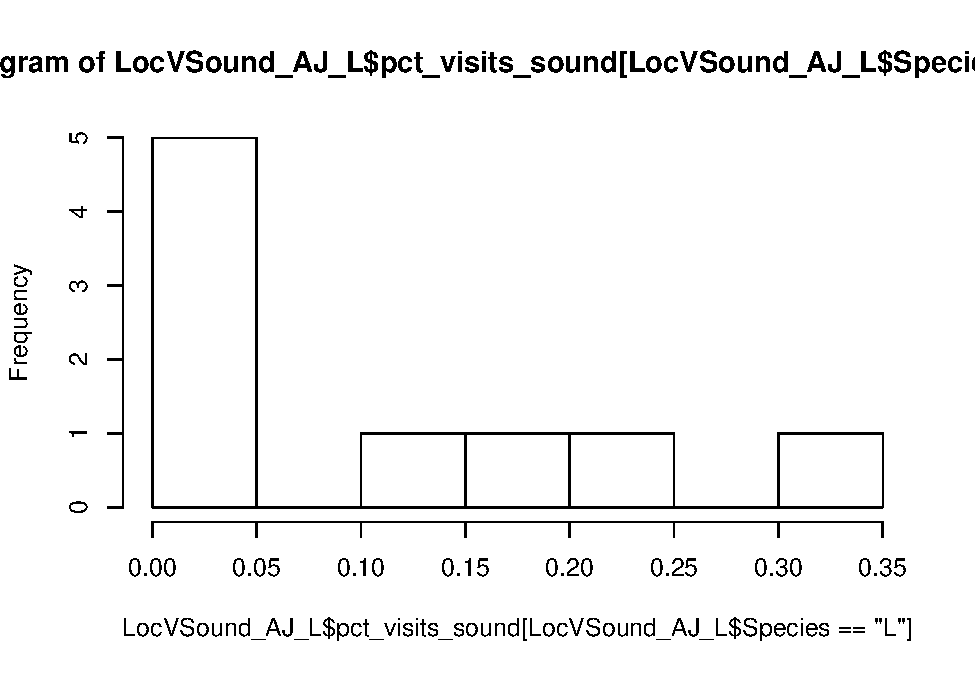
\includegraphics{Sensory_learning_files/figure-latex/unnamed-chunk-7-1.pdf}

\begin{Shaded}
\begin{Highlighting}[]
\CommentTok{#not particularly normal}
\KeywordTok{head}\NormalTok{(LocVSound_AJ_L)}
\end{Highlighting}
\end{Shaded}

\begin{verbatim}
##     Bat.ID  Scorer    Date  Time Species      Test Rewarded_loc
## 1   A-C095 unknown  4/1/17     1      AJ LocVSound          4,2
## 2   D-C0B6 unknown  4/2/17 23:45      AJ LocVSound          4,2
## 3   K-C091     May 4/30/17 21:47      AJ LocVSound          3,3
## 4   B-Butt   Dylan  7/1/17 21:37       L LocVSound          3,1
## 5 C-Newbie   Dylan  7/1/17 19:12       L LocVSound          3,2
## 7   B-C09E   Dylan  4/5/17 19:41      AJ LocVSound          4,2
##   Rewarded_sound first_hover first_land first_visit lands_loc hovers_loc
## 1        epsilon    location   location    location         1         10
## 2        epsilon     neither   location     neither         5          1
## 3           feta    location       <NA>    location         0         13
## 4           feta    location   location    location         0          5
## 5           feta    location   location    location        15          7
## 7        epsilon         NA        <NA>        <NA>         0          0
##   visits_loc lands_sound hovers_sound visits_sound lands_neither
## 1         11           0            0            0             0
## 2          6           0            0            0             0
## 3         13           0            1            1             0
## 4          5           0            0            0             0
## 5         22           0            0            0             0
## 7          0           0            0            0             0
##   hovers_neither visits_neither lands_nearest hovers_nearest
## 1              1              1             0              1
## 2              5              5            NA           <NA>
## 3              5              5             0              0
## 4              0              0             0              1
## 5              0              0            NA           <NA>
## 7              0              0             0              0
##   visits_nearest lands_alpha hovers_alpha visits_alpha lands_beta
## 1              1          NA           NA           NA          0
## 2             NA          NA           NA           NA          5
## 3              0           0            5            5         NA
## 4              1           0            5            5         NA
## 5             NA           0            0            0         15
## 7              0           0            0            0          0
##   hovers_beta visits_beta lands_feta hovers_feta visits_feta lands_epsilon
## 1           1           1          1          10          11             0
## 2           1           6          0           5           5             0
## 3          NA          NA          0           1           1             0
## 4          NA          NA          0           1           1             0
## 5           7          22          0           0           0             0
## 7           0           0          0           0           0             0
##   hovers_epsilon visits_epsilon total_lands total_hovers total_visits
## 1              0              0           1           11           12
## 2              0              0           5            6           11
## 3             13             13           0           19           19
## 4              0              0           0            5            6
## 5              0              0          15            7           22
## 7              0              0           0            0            0
##   pct_visits_loc pct_visits_sound pct_visits_neither
## 1      0.9166667       0.00000000         0.08333333
## 2      0.5454545       0.00000000         0.45454545
## 3      0.6842105       0.05263158         0.26315789
## 4      0.8333333       0.00000000         0.00000000
## 5      1.0000000       0.00000000         0.00000000
## 7             NA               NA                 NA
\end{verbatim}

Do AJs go to one platform more than another? Do Lophostoma go to any
platforms more than one another? Which? Is there a difference between
AJs and lophostoma? (anova? )

\paragraph{Reshape data for plotting and manipulation with
percents}\label{reshape-data-for-plotting-and-manipulation-with-percents}

\begin{Shaded}
\begin{Highlighting}[]
\CommentTok{# pull out just the relevent columns: }
\NormalTok{LocVSound_AJ_L_pcts<-}\StringTok{ }\NormalTok{LocVSound_AJ_L[ , }\KeywordTok{c}\NormalTok{(}\StringTok{"Bat.ID"}\NormalTok{, }\StringTok{"Species"}\NormalTok{, }\StringTok{"pct_visits_loc"}\NormalTok{, }\StringTok{"pct_visits_sound"}\NormalTok{, }\StringTok{"pct_visits_neither"}\NormalTok{)]}
\KeywordTok{head}\NormalTok{(LocVSound_AJ_L_pcts)}
\end{Highlighting}
\end{Shaded}

\begin{verbatim}
##     Bat.ID Species pct_visits_loc pct_visits_sound pct_visits_neither
## 1   A-C095      AJ      0.9166667       0.00000000         0.08333333
## 2   D-C0B6      AJ      0.5454545       0.00000000         0.45454545
## 3   K-C091      AJ      0.6842105       0.05263158         0.26315789
## 4   B-Butt       L      0.8333333       0.00000000         0.00000000
## 5 C-Newbie       L      1.0000000       0.00000000         0.00000000
## 7   B-C09E      AJ             NA               NA                 NA
\end{verbatim}

\begin{Shaded}
\begin{Highlighting}[]
\NormalTok{## Alternatively could just put all the rows I don't want melted into "id" in the following fuction. }
\KeywordTok{colnames}\NormalTok{(LocVSound_AJ_L_pcts)}
\end{Highlighting}
\end{Shaded}

\begin{verbatim}
## [1] "Bat.ID"             "Species"            "pct_visits_loc"    
## [4] "pct_visits_sound"   "pct_visits_neither"
\end{verbatim}

\begin{Shaded}
\begin{Highlighting}[]
\NormalTok{mLocVSound <-}\StringTok{ }\KeywordTok{melt}\NormalTok{(LocVSound_AJ_L_pcts, }\DataTypeTok{id=}\KeywordTok{c}\NormalTok{(}\StringTok{"Bat.ID"}\NormalTok{,}\StringTok{"Species"}\NormalTok{))}
\KeywordTok{hist}\NormalTok{(mLocVSound$value)}
\end{Highlighting}
\end{Shaded}

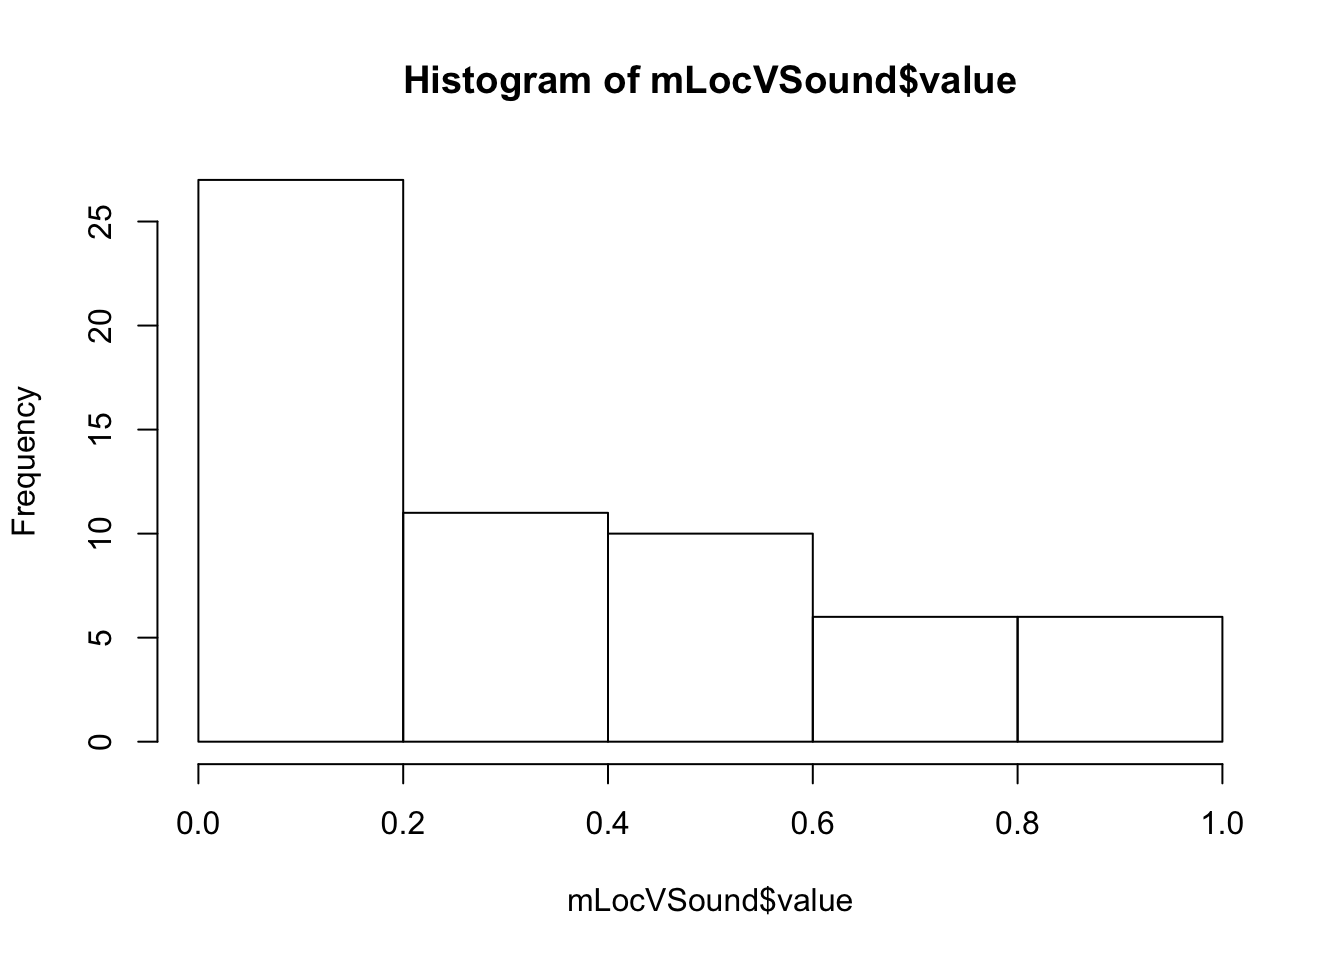
\includegraphics{Sensory_learning_files/figure-latex/unnamed-chunk-8-1.pdf}

\begin{Shaded}
\begin{Highlighting}[]
\KeywordTok{head}\NormalTok{(mLocVSound)}
\end{Highlighting}
\end{Shaded}

\begin{verbatim}
##     Bat.ID Species       variable     value
## 1   A-C095      AJ pct_visits_loc 0.9166667
## 2   D-C0B6      AJ pct_visits_loc 0.5454545
## 3   K-C091      AJ pct_visits_loc 0.6842105
## 4   B-Butt       L pct_visits_loc 0.8333333
## 5 C-Newbie       L pct_visits_loc 1.0000000
## 6   B-C09E      AJ pct_visits_loc        NA
\end{verbatim}

\begin{Shaded}
\begin{Highlighting}[]
\CommentTok{#rm(mLocVSound )}
\end{Highlighting}
\end{Shaded}

\paragraph{Reshape data for plotting and manipulation with
COUNTS}\label{reshape-data-for-plotting-and-manipulation-with-counts}

\begin{Shaded}
\begin{Highlighting}[]
\CommentTok{# pull out just the relevent columns: }
\NormalTok{LocVSound_AJ_L_cnts<-}\StringTok{ }\NormalTok{LocVSound_AJ_L[ , }\KeywordTok{c}\NormalTok{(}\StringTok{"Bat.ID"}\NormalTok{, }\StringTok{"Species"}\NormalTok{, }\StringTok{"visits_loc"}\NormalTok{, }\StringTok{"visits_sound"}\NormalTok{, }\StringTok{"visits_neither"}\NormalTok{)]}
\KeywordTok{head}\NormalTok{(LocVSound_AJ_L_cnts)}
\end{Highlighting}
\end{Shaded}

\begin{verbatim}
##     Bat.ID Species visits_loc visits_sound visits_neither
## 1   A-C095      AJ         11            0              1
## 2   D-C0B6      AJ          6            0              5
## 3   K-C091      AJ         13            1              5
## 4   B-Butt       L          5            0              0
## 5 C-Newbie       L         22            0              0
## 7   B-C09E      AJ          0            0              0
\end{verbatim}

\begin{Shaded}
\begin{Highlighting}[]
\NormalTok{## Alternatively could just put all the rows I don't want melted into "id" in the following fuction, which would save the rest of the data}
\KeywordTok{colnames}\NormalTok{(LocVSound_AJ_L_cnts)}
\end{Highlighting}
\end{Shaded}

\begin{verbatim}
## [1] "Bat.ID"         "Species"        "visits_loc"     "visits_sound"  
## [5] "visits_neither"
\end{verbatim}

\begin{Shaded}
\begin{Highlighting}[]
\NormalTok{mLocVSound_cnts <-}\StringTok{ }\KeywordTok{melt}\NormalTok{(LocVSound_AJ_L_cnts, }\DataTypeTok{id=}\KeywordTok{c}\NormalTok{(}\StringTok{"Bat.ID"}\NormalTok{,}\StringTok{"Species"}\NormalTok{))}
\KeywordTok{head}\NormalTok{(mLocVSound_cnts)}
\end{Highlighting}
\end{Shaded}

\begin{verbatim}
##     Bat.ID Species   variable value
## 1   A-C095      AJ visits_loc    11
## 2   D-C0B6      AJ visits_loc     6
## 3   K-C091      AJ visits_loc    13
## 4   B-Butt       L visits_loc     5
## 5 C-Newbie       L visits_loc    22
## 6   B-C09E      AJ visits_loc     0
\end{verbatim}

\begin{Shaded}
\begin{Highlighting}[]
\NormalTok{## convenient also to just add this count value to mLocvSound}
\NormalTok{visits_counts<-mLocVSound_cnts$value}
\NormalTok{mLocVSound <-}\KeywordTok{cbind}\NormalTok{(mLocVSound, visits_counts)}
\end{Highlighting}
\end{Shaded}

" Did the bats fly to the three platforms the same amount? (W/in
species): independent variables: 1: cue (3 levels) dependent variables:
1: percent visits by bat, not independent AJS \#\#\#\# Kruskal-wallace:
AJ

\begin{Shaded}
\begin{Highlighting}[]
\NormalTok{LvS_AJ_k.test<-}\StringTok{ }\KeywordTok{kruskal.test}\NormalTok{(value ~}\StringTok{ }\NormalTok{variable, }\DataTypeTok{data =}\NormalTok{mLocVSound[mLocVSound$Species ==}\StringTok{"AJ"}\NormalTok{, ] )}

\NormalTok{LvS_AJ_k.test}
\end{Highlighting}
\end{Shaded}

\begin{verbatim}
## 
##  Kruskal-Wallis rank sum test
## 
## data:  value by variable
## Kruskal-Wallis chi-squared = 16.419, df = 2, p-value = 0.000272
\end{verbatim}

Significant difference, bats did not fly to the three platforms equally,
so post-hocs

\paragraph{Kruskal-wallace: Lophos}\label{kruskal-wallace-lophos}

\begin{Shaded}
\begin{Highlighting}[]
\NormalTok{LvS_L_k.test<-}\StringTok{ }\KeywordTok{kruskal.test}\NormalTok{(value ~}\StringTok{ }\NormalTok{variable, }\DataTypeTok{data =}\NormalTok{mLocVSound[mLocVSound$Species ==}\StringTok{"L"}\NormalTok{, ] )}

\NormalTok{LvS_L_k.test}
\end{Highlighting}
\end{Shaded}

\begin{verbatim}
## 
##  Kruskal-Wallis rank sum test
## 
## data:  value by variable
## Kruskal-Wallis chi-squared = 17.809, df = 2, p-value = 0.0001358
\end{verbatim}

Significant difference, so post-hocs

``Which platforms did the bats fly to more, which were different?''

\paragraph{Man- Whitney / Wilcox: AJs}\label{man--whitney-wilcox-ajs}

\begin{Shaded}
\begin{Highlighting}[]
\NormalTok{LvS_AJ_wilhox =}\StringTok{ }\KeywordTok{pairwise.wilcox.test}\NormalTok{(mLocVSound[mLocVSound$Species ==}\StringTok{"AJ"}\NormalTok{, ]$value,  mLocVSound[mLocVSound$Species ==}\StringTok{"AJ"}\NormalTok{, ]$variable, }\DataTypeTok{p.adjust.method=}\NormalTok{p.adjust.methods)}
\end{Highlighting}
\end{Shaded}

\begin{verbatim}
## Warning in wilcox.test.default(xi, xj, paired = paired, ...): cannot
## compute exact p-value with ties

## Warning in wilcox.test.default(xi, xj, paired = paired, ...): cannot
## compute exact p-value with ties
\end{verbatim}

\begin{Shaded}
\begin{Highlighting}[]
\NormalTok{LvS_AJ_wilhox}
\end{Highlighting}
\end{Shaded}

\begin{verbatim}
## 
##  Pairwise comparisons using Wilcoxon rank sum test 
## 
## data:  mLocVSound[mLocVSound$Species == "AJ", ]$value and mLocVSound[mLocVSound$Species == "AJ", ]$variable 
## 
##                    pct_visits_loc pct_visits_sound
## pct_visits_sound   0.0015         -               
## pct_visits_neither 0.0015         0.1473          
## 
## P value adjustment method: holm
\end{verbatim}

AJs visited the location significantly more than they visited the sound
or the control platform, there was no detectable difference between
percent visits to sound or neither

\paragraph{Man- Whitney / Wilcox:
Lophos}\label{man--whitney-wilcox-lophos}

\begin{Shaded}
\begin{Highlighting}[]
\NormalTok{LvS_L_wilhox =}\StringTok{ }\KeywordTok{pairwise.wilcox.test}\NormalTok{(mLocVSound[mLocVSound$Species ==}\StringTok{"L"}\NormalTok{, ]$value,  mLocVSound[mLocVSound$Species ==}\StringTok{"L"}\NormalTok{, ]$variable, }\DataTypeTok{p.adjust.method=}\NormalTok{p.adjust.methods)}
\end{Highlighting}
\end{Shaded}

\begin{verbatim}
## Warning in wilcox.test.default(xi, xj, paired = paired, ...): cannot
## compute exact p-value with ties

## Warning in wilcox.test.default(xi, xj, paired = paired, ...): cannot
## compute exact p-value with ties

## Warning in wilcox.test.default(xi, xj, paired = paired, ...): cannot
## compute exact p-value with ties
\end{verbatim}

\begin{Shaded}
\begin{Highlighting}[]
\NormalTok{LvS_L_wilhox}
\end{Highlighting}
\end{Shaded}

\begin{verbatim}
## 
##  Pairwise comparisons using Wilcoxon rank sum test 
## 
## data:  mLocVSound[mLocVSound$Species == "L", ]$value and mLocVSound[mLocVSound$Species == "L", ]$variable 
## 
##                    pct_visits_loc pct_visits_sound
## pct_visits_sound   0.0011         -               
## pct_visits_neither 0.0011         1.0000          
## 
## P value adjustment method: holm
\end{verbatim}

Same with Lophostoma, they were significantly more likely to visit
location, over sound or the control, no difference between those.

\subsection{Dunn test post hoc: AJ}\label{dunn-test-post-hoc-aj}

\begin{Shaded}
\begin{Highlighting}[]
\NormalTok{LvS_AJ_dunn<-}\KeywordTok{dunnTest}\NormalTok{(mLocVSound[mLocVSound$Species ==}\StringTok{"AJ"}\NormalTok{, ]$value,  mLocVSound[mLocVSound$Species ==}\StringTok{"AJ"}\NormalTok{, ]$variable, }\DataTypeTok{method=}\StringTok{"holm"}\NormalTok{, }\DataTypeTok{kw=}\OtherTok{TRUE}\NormalTok{)}
\end{Highlighting}
\end{Shaded}

\begin{verbatim}
## Warning: Some rows deleted from 'x' and 'g' because missing data.
\end{verbatim}

\begin{Shaded}
\begin{Highlighting}[]
\NormalTok{LvS_AJ_dunn}
\end{Highlighting}
\end{Shaded}

\begin{verbatim}
## Dunn (1964) Kruskal-Wallis multiple comparison
\end{verbatim}

\begin{verbatim}
##   p-values adjusted with the Holm method.
\end{verbatim}

\begin{verbatim}
##                              Comparison        Z      P.unadj        P.adj
## 1   pct_visits_loc - pct_visits_neither 2.824830 4.730567e-03 0.0094611334
## 2     pct_visits_loc - pct_visits_sound 3.928280 8.555571e-05 0.0002566671
## 3 pct_visits_neither - pct_visits_sound 1.103449 2.698321e-01 0.2698320863
\end{verbatim}

\subsection{Dunn test post hoc: Lopho}\label{dunn-test-post-hoc-lopho}

\begin{Shaded}
\begin{Highlighting}[]
\NormalTok{LvS_L_dunn<-}\KeywordTok{dunnTest}\NormalTok{(mLocVSound[mLocVSound$Species ==}\StringTok{"L"}\NormalTok{, ]$value,  mLocVSound[mLocVSound$Species ==}\StringTok{"L"}\NormalTok{, ]$variable, }\DataTypeTok{method=}\StringTok{"holm"}\NormalTok{, }\DataTypeTok{kw=}\OtherTok{TRUE}\NormalTok{)}
\NormalTok{LvS_L_dunn}
\end{Highlighting}
\end{Shaded}

\begin{verbatim}
## Dunn (1964) Kruskal-Wallis multiple comparison
\end{verbatim}

\begin{verbatim}
##   p-values adjusted with the Holm method.
\end{verbatim}

\begin{verbatim}
##                              Comparison          Z      P.unadj
## 1   pct_visits_loc - pct_visits_neither 3.63174896 0.0002815069
## 2     pct_visits_loc - pct_visits_sound 3.67714582 0.0002358582
## 3 pct_visits_neither - pct_visits_sound 0.04539686 0.9637909822
##          P.adj
## 1 0.0005630138
## 2 0.0007075747
## 3 0.9637909822
\end{verbatim}

\paragraph{Nemenyi or Zar or Mann-Whitney tests for post hoc
analyses?}\label{nemenyi-or-zar-or-mann-whitney-tests-for-post-hoc-analyses}

\paragraph{Do the different species go to the platforms
equally?}\label{do-the-different-species-go-to-the-platforms-equally}

Independent variables: species (categorical, 2 levels) cue (categorical,
2 levels) Dependent variables: \# visits, proportion visits

No good non-parametric option for a 2 way anova.

\subsection{Investigating assumptions for ANOVA Trying out
transformations}\label{investigating-assumptions-for-anova-trying-out-transformations}

\begin{Shaded}
\begin{Highlighting}[]
\CommentTok{#proportion data}
\KeywordTok{boxplot}\NormalTok{(value ~}\StringTok{  }\NormalTok{variable*}\StringTok{ }\NormalTok{Species, }\DataTypeTok{data =} \NormalTok{mLocVSound) }\CommentTok{#box width of largest looks more than 2x larger than that of smaller}
\KeywordTok{bartlett.test}\NormalTok{( value ~}\StringTok{  }\KeywordTok{interaction}\NormalTok{(variable, Species), }\DataTypeTok{data =} \NormalTok{mLocVSound) }\CommentTok{#Bartlett test shows variances arn't so different}
\end{Highlighting}
\end{Shaded}

\begin{verbatim}
## 
##  Bartlett test of homogeneity of variances
## 
## data:  value by interaction(variable, Species)
## Bartlett's K-squared = 4.0889, df = 5, p-value = 0.5367
\end{verbatim}

\begin{Shaded}
\begin{Highlighting}[]
\CommentTok{# proportions don't have normal variance}

\CommentTok{# Count data also does not have homogenaity of variances boxplot(value ~  variable* Species, data = mLocVSound_cnts)}
\KeywordTok{bartlett.test}\NormalTok{( value ~}\StringTok{  }\KeywordTok{interaction}\NormalTok{(variable, Species), }\DataTypeTok{data =} \NormalTok{mLocVSound_cnts)}
\end{Highlighting}
\end{Shaded}

\begin{verbatim}
## 
##  Bartlett test of homogeneity of variances
## 
## data:  value by interaction(variable, Species)
## Bartlett's K-squared = 34.198, df = 5, p-value = 2.175e-06
\end{verbatim}

\begin{Shaded}
\begin{Highlighting}[]
\CommentTok{# does not have homogenaity of variance}

\CommentTok{# Proportion data transformations #}
\NormalTok{mLocVSound$value_sqrt<-}\StringTok{ }\NormalTok{(}\KeywordTok{sqrt}\NormalTok{(mLocVSound$value)) }\CommentTok{#sqrt transformation}
\NormalTok{mLocVSound$value_cub =}\StringTok{ }\KeywordTok{sign}\NormalTok{(mLocVSound$value) *}\StringTok{ }\KeywordTok{abs}\NormalTok{(mLocVSound$value)^(}\DecValTok{1}\NormalTok{/}\DecValTok{3}\NormalTok{)  }\CommentTok{#cubed transformation}
\NormalTok{mLocVSound$value_log<-}\StringTok{ }\NormalTok{(}\KeywordTok{log}\NormalTok{(mLocVSound$value))}\CommentTok{#log transformation- too strong}

\CommentTok{# Count data transformations #}
\NormalTok{mLocVSound_cnts$value_sqrt<-}\StringTok{ }\NormalTok{(}\KeywordTok{sqrt}\NormalTok{(mLocVSound_cnts$value)) }\CommentTok{#sqrt transformation}
\NormalTok{mLocVSound_cnts$value_cub =}\StringTok{ }\KeywordTok{sign}\NormalTok{(mLocVSound_cnts$value) *}\StringTok{ }\KeywordTok{abs}\NormalTok{(mLocVSound_cnts$value)^(}\DecValTok{1}\NormalTok{/}\DecValTok{3}\NormalTok{)  }\CommentTok{#cubed transformation}
\NormalTok{mLocVSound_cnts$value_log<-}\StringTok{ }\NormalTok{(}\KeywordTok{log}\NormalTok{(mLocVSound_cnts$value))}\CommentTok{#log transformation- too strong}

\CommentTok{#  Proportion data boxplots #}
\KeywordTok{boxplot}\NormalTok{(value ~}\StringTok{  }\NormalTok{variable*}\StringTok{ }\NormalTok{Species, }\DataTypeTok{data =} \NormalTok{mLocVSound) }\CommentTok{#original}
\end{Highlighting}
\end{Shaded}

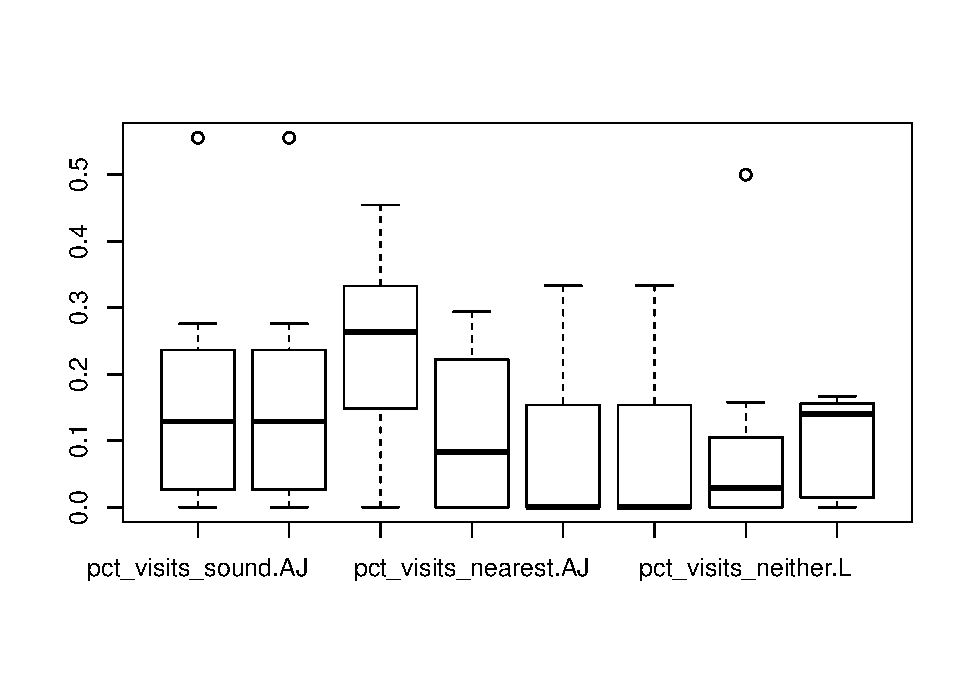
\includegraphics{Sensory_learning_files/figure-latex/unnamed-chunk-17-1.pdf}

\begin{Shaded}
\begin{Highlighting}[]
\CommentTok{#ok}
\KeywordTok{boxplot}\NormalTok{(value_sqrt ~}\StringTok{  }\NormalTok{variable*}\StringTok{ }\NormalTok{Species, }\DataTypeTok{data =} \NormalTok{mLocVSound) }\CommentTok{#sqrt}
\end{Highlighting}
\end{Shaded}

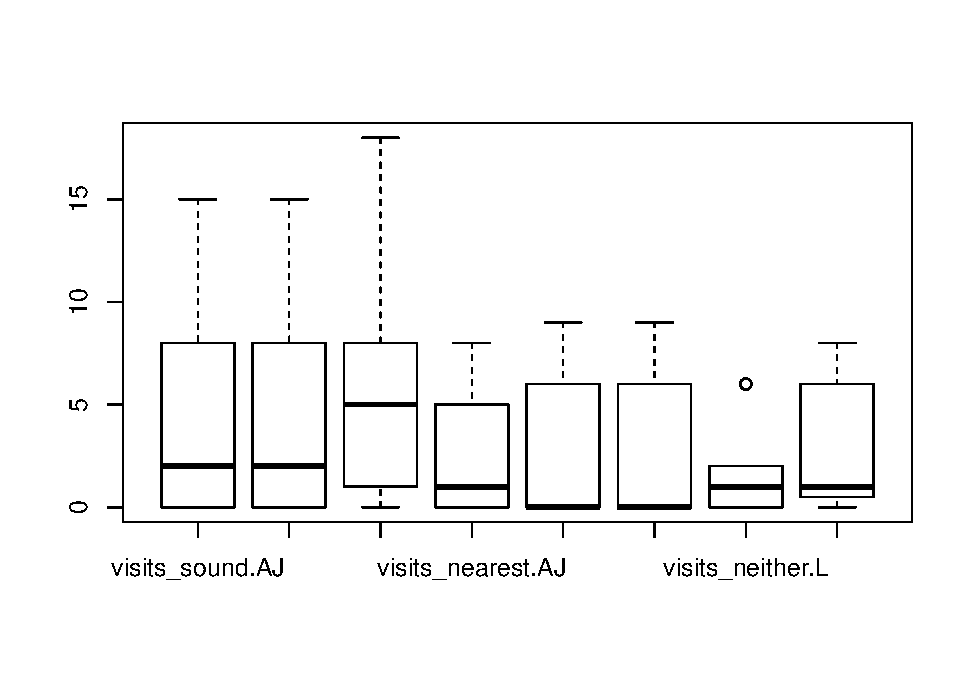
\includegraphics{Sensory_learning_files/figure-latex/unnamed-chunk-17-2.pdf}

\begin{Shaded}
\begin{Highlighting}[]
\NormalTok{##pretty good}
\KeywordTok{boxplot}\NormalTok{(value_cub ~}\StringTok{  }\NormalTok{variable*}\StringTok{ }\NormalTok{Species, }\DataTypeTok{data =} \NormalTok{mLocVSound) }\CommentTok{#cub, less good}
\end{Highlighting}
\end{Shaded}

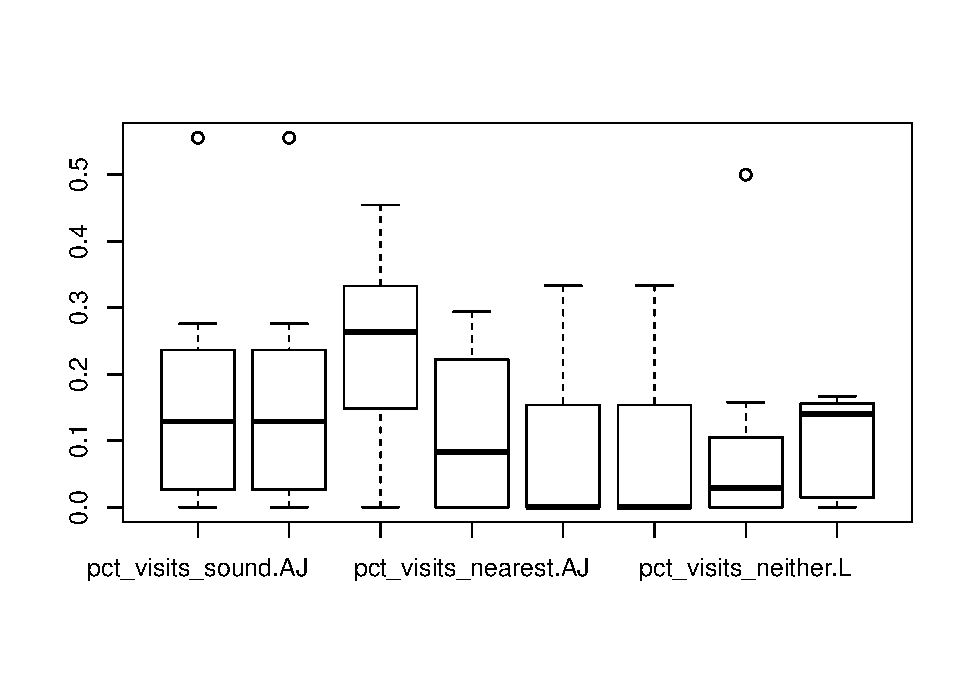
\includegraphics{Sensory_learning_files/figure-latex/unnamed-chunk-17-3.pdf}

\begin{Shaded}
\begin{Highlighting}[]
\KeywordTok{boxplot}\NormalTok{(value_log ~}\StringTok{  }\NormalTok{variable*}\StringTok{ }\NormalTok{Species, }\DataTypeTok{data =} \NormalTok{mLocVSound) }\CommentTok{# too strong}
\end{Highlighting}
\end{Shaded}

\begin{verbatim}
## Warning in bplt(at[i], wid = width[i], stats = z$stats[, i], out =
## z$out[z$group == : Outlier (-Inf) in boxplot 3 is not drawn
\end{verbatim}

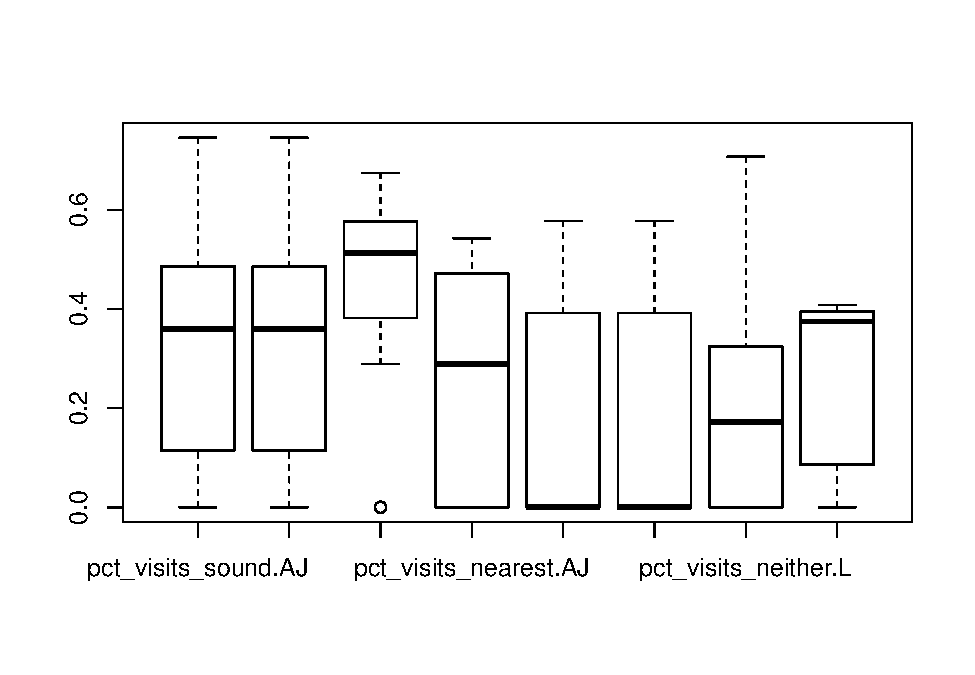
\includegraphics{Sensory_learning_files/figure-latex/unnamed-chunk-17-4.pdf}

\begin{Shaded}
\begin{Highlighting}[]
\CommentTok{#Count data boxplots #}
\KeywordTok{boxplot}\NormalTok{(value ~}\StringTok{  }\NormalTok{variable*}\StringTok{ }\NormalTok{Species, }\DataTypeTok{data =} \NormalTok{mLocVSound_cnts) }\CommentTok{#unequal variance}
\end{Highlighting}
\end{Shaded}

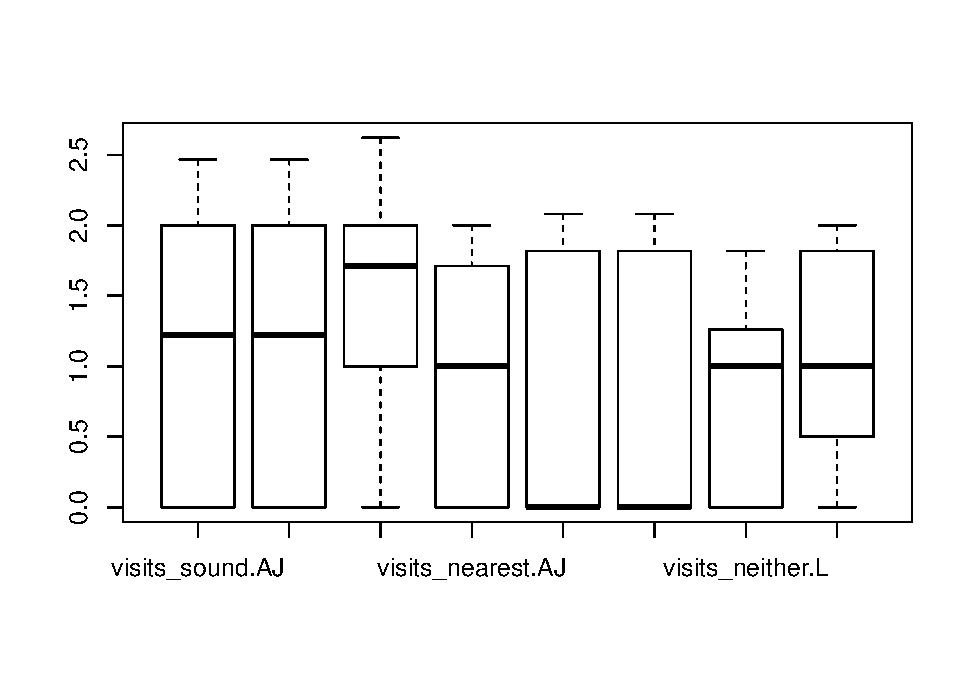
\includegraphics{Sensory_learning_files/figure-latex/unnamed-chunk-17-5.pdf}

\begin{Shaded}
\begin{Highlighting}[]
\KeywordTok{boxplot}\NormalTok{(value_sqrt ~}\StringTok{  }\NormalTok{variable*}\StringTok{ }\NormalTok{Species, }\DataTypeTok{data =} \NormalTok{mLocVSound_cnts) }\CommentTok{#sqrt, pretty good}
\end{Highlighting}
\end{Shaded}

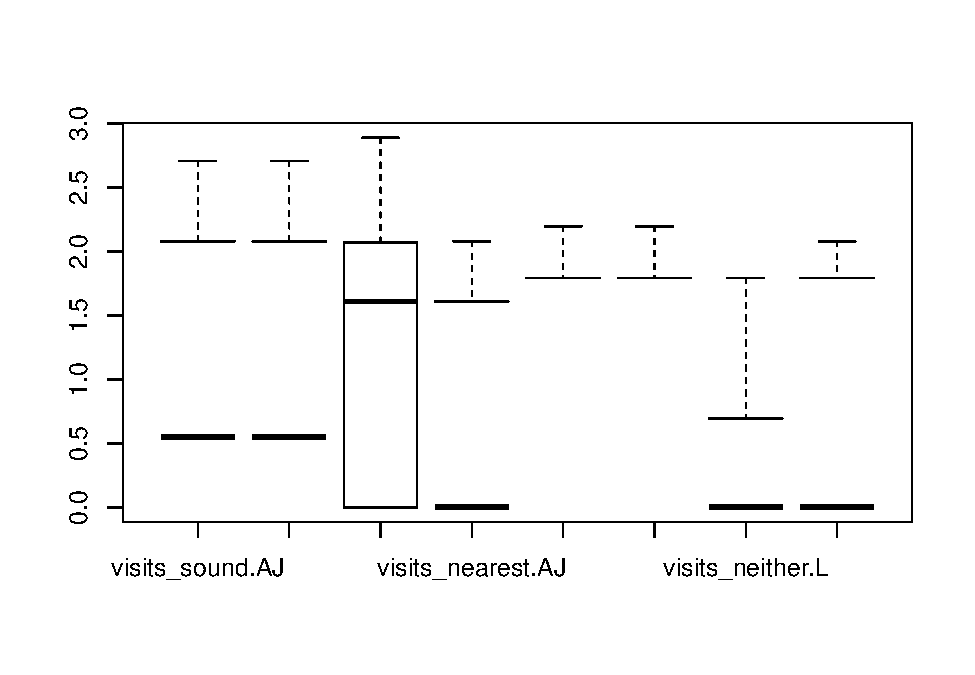
\includegraphics{Sensory_learning_files/figure-latex/unnamed-chunk-17-6.pdf}

\begin{Shaded}
\begin{Highlighting}[]
\KeywordTok{boxplot}\NormalTok{(value_cub ~}\StringTok{  }\NormalTok{variable*}\StringTok{ }\NormalTok{Species, }\DataTypeTok{data =} \NormalTok{mLocVSound_cnts) }\CommentTok{#cub, pretty good}
\end{Highlighting}
\end{Shaded}

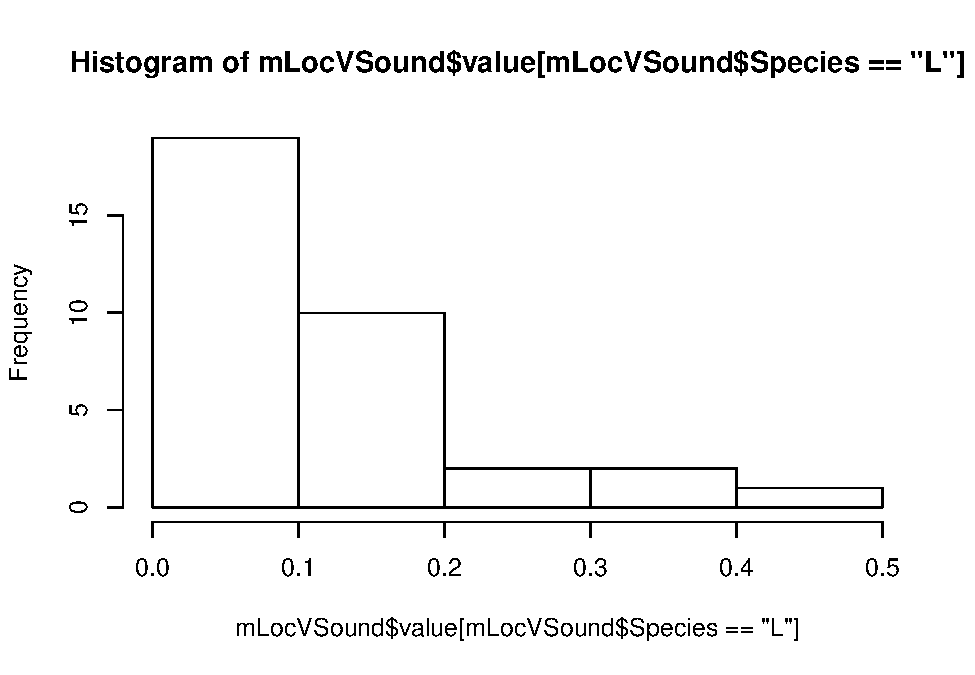
\includegraphics{Sensory_learning_files/figure-latex/unnamed-chunk-17-7.pdf}

\begin{Shaded}
\begin{Highlighting}[]
\KeywordTok{boxplot}\NormalTok{(value_log ~}\StringTok{  }\NormalTok{variable*}\StringTok{ }\NormalTok{Species, }\DataTypeTok{data =} \NormalTok{mLocVSound_cnts) }\CommentTok{# too strong}
\end{Highlighting}
\end{Shaded}

\begin{verbatim}
## Warning in bplt(at[i], wid = width[i], stats = z$stats[, i], out =
## z$out[z$group == : Outlier (-Inf) in boxplot 1 is not drawn

## Warning in bplt(at[i], wid = width[i], stats = z$stats[, i], out =
## z$out[z$group == : Outlier (-Inf) in boxplot 3 is not drawn
\end{verbatim}

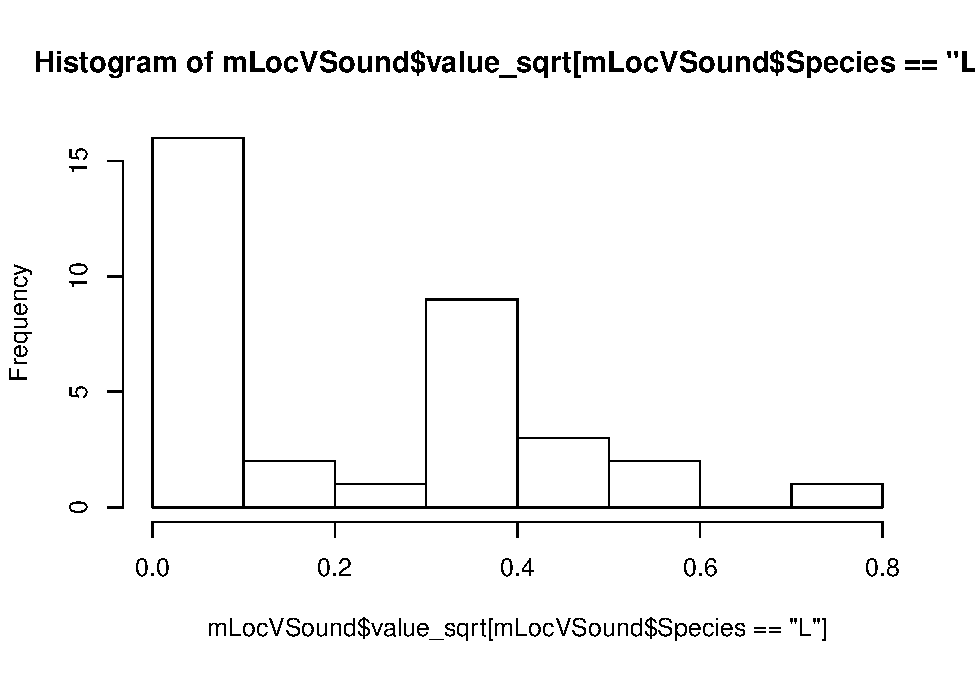
\includegraphics{Sensory_learning_files/figure-latex/unnamed-chunk-17-8.pdf}

\begin{Shaded}
\begin{Highlighting}[]
\KeywordTok{bartlett.test}\NormalTok{( value_log ~}\StringTok{  }\KeywordTok{interaction}\NormalTok{(variable, Species), }\DataTypeTok{data =} \NormalTok{mLocVSound_cnts)}
\end{Highlighting}
\end{Shaded}

\begin{verbatim}
## 
##  Bartlett test of homogeneity of variances
## 
## data:  value_log by interaction(variable, Species)
## Bartlett's K-squared = NaN, df = 5, p-value = NA
\end{verbatim}

\begin{Shaded}
\begin{Highlighting}[]
\NormalTok{## This actually seems to have fixed the homogenaity of variances problem}

\CommentTok{#normality? Less important, ANOVAs are robust against this violation}
\CommentTok{#proportions: }
\KeywordTok{hist}\NormalTok{(mLocVSound$value[mLocVSound$Species==}\StringTok{"L"}\NormalTok{], }\DataTypeTok{breaks=}\DecValTok{6}\NormalTok{)}
\end{Highlighting}
\end{Shaded}

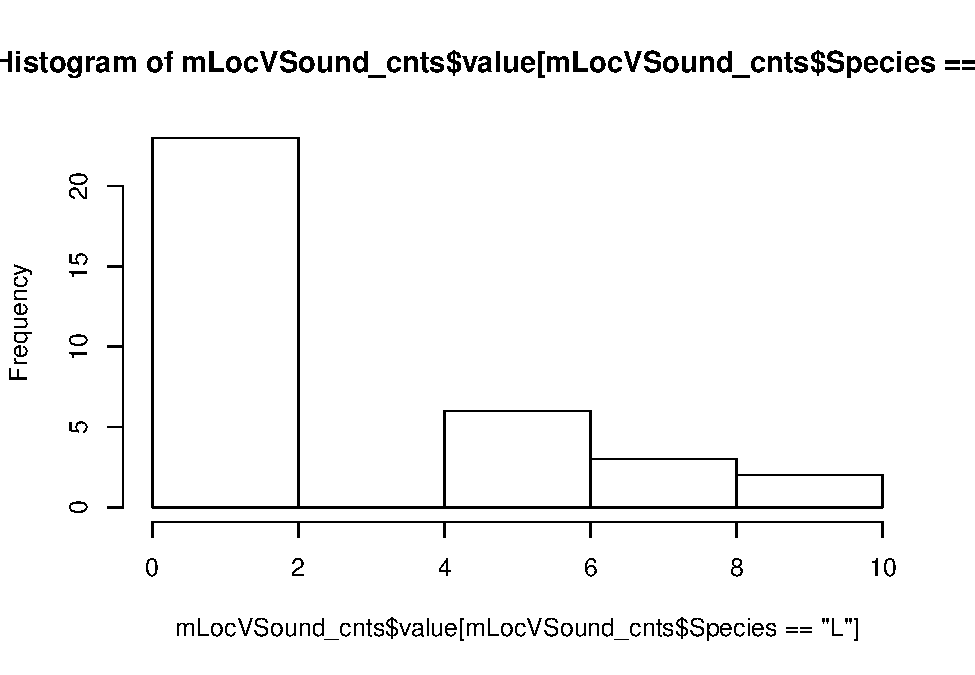
\includegraphics{Sensory_learning_files/figure-latex/unnamed-chunk-17-9.pdf}

\begin{Shaded}
\begin{Highlighting}[]
\KeywordTok{hist}\NormalTok{(mLocVSound$value_sqrt[mLocVSound$Species==}\StringTok{"L"}\NormalTok{], }\DataTypeTok{breaks=}\DecValTok{6}\NormalTok{)}
\end{Highlighting}
\end{Shaded}

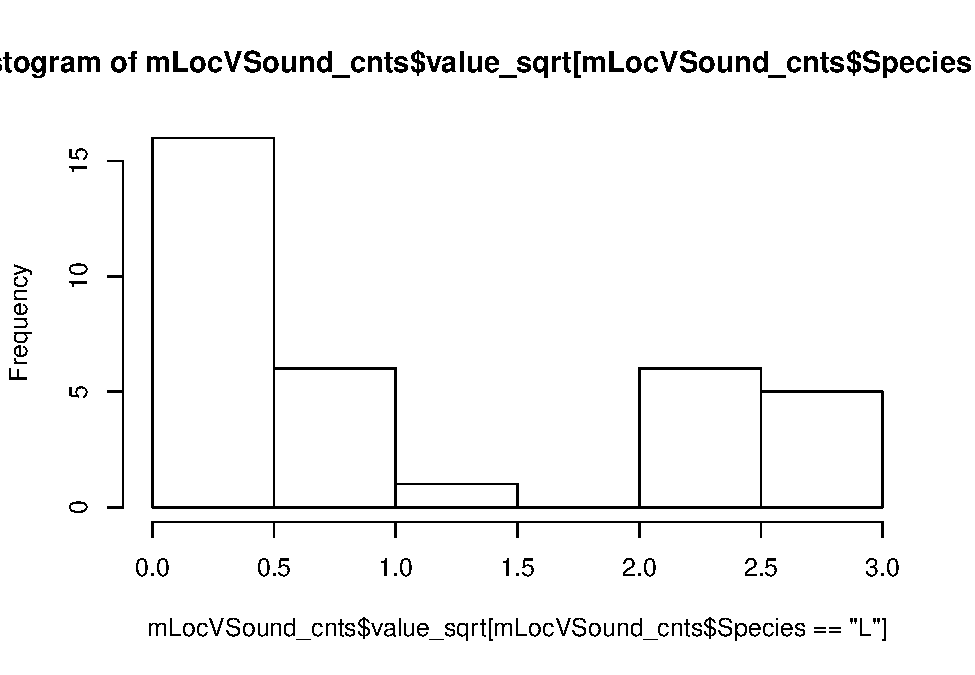
\includegraphics{Sensory_learning_files/figure-latex/unnamed-chunk-17-10.pdf}

\begin{Shaded}
\begin{Highlighting}[]
\CommentTok{#hist(mLocVSound$value_cub[mLocVSound$Species=="L"], breaks=6)}


\CommentTok{#counts:}
\KeywordTok{hist}\NormalTok{(mLocVSound_cnts$value[mLocVSound_cnts$Species==}\StringTok{"L"}\NormalTok{], }\DataTypeTok{breaks=}\DecValTok{6}\NormalTok{)}
\end{Highlighting}
\end{Shaded}

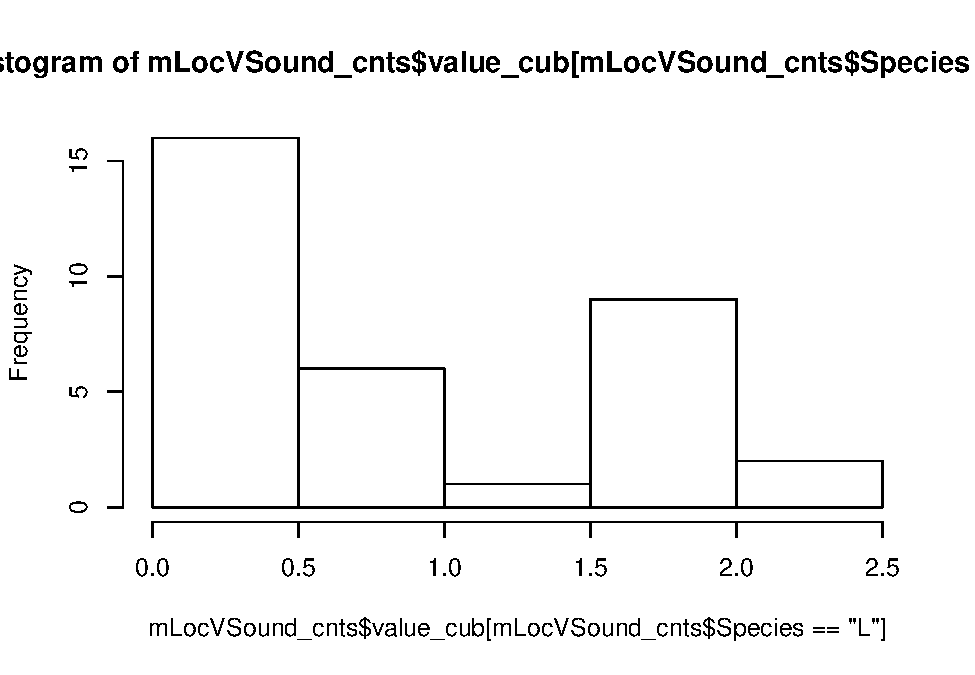
\includegraphics{Sensory_learning_files/figure-latex/unnamed-chunk-17-11.pdf}

\begin{Shaded}
\begin{Highlighting}[]
\KeywordTok{hist}\NormalTok{(mLocVSound_cnts$value_sqrt[mLocVSound_cnts$Species==}\StringTok{"L"}\NormalTok{], }\DataTypeTok{breaks=}\DecValTok{6}\NormalTok{)}
\end{Highlighting}
\end{Shaded}

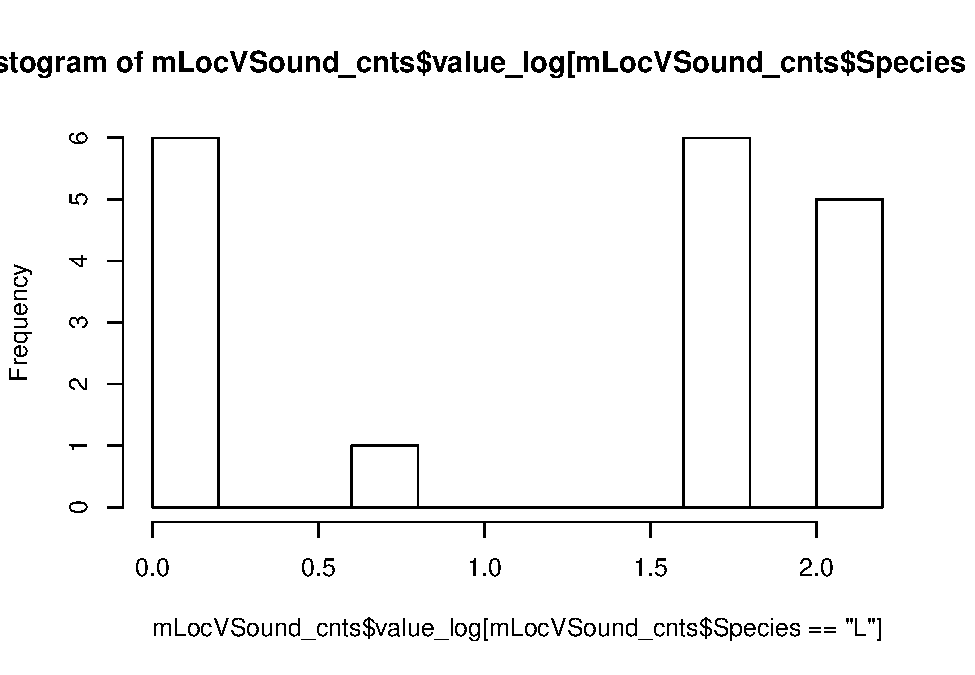
\includegraphics{Sensory_learning_files/figure-latex/unnamed-chunk-17-12.pdf}

\begin{Shaded}
\begin{Highlighting}[]
\KeywordTok{hist}\NormalTok{(mLocVSound_cnts$value_cub[mLocVSound_cnts$Species==}\StringTok{"L"}\NormalTok{], }\DataTypeTok{breaks=}\DecValTok{6}\NormalTok{)}
\end{Highlighting}
\end{Shaded}

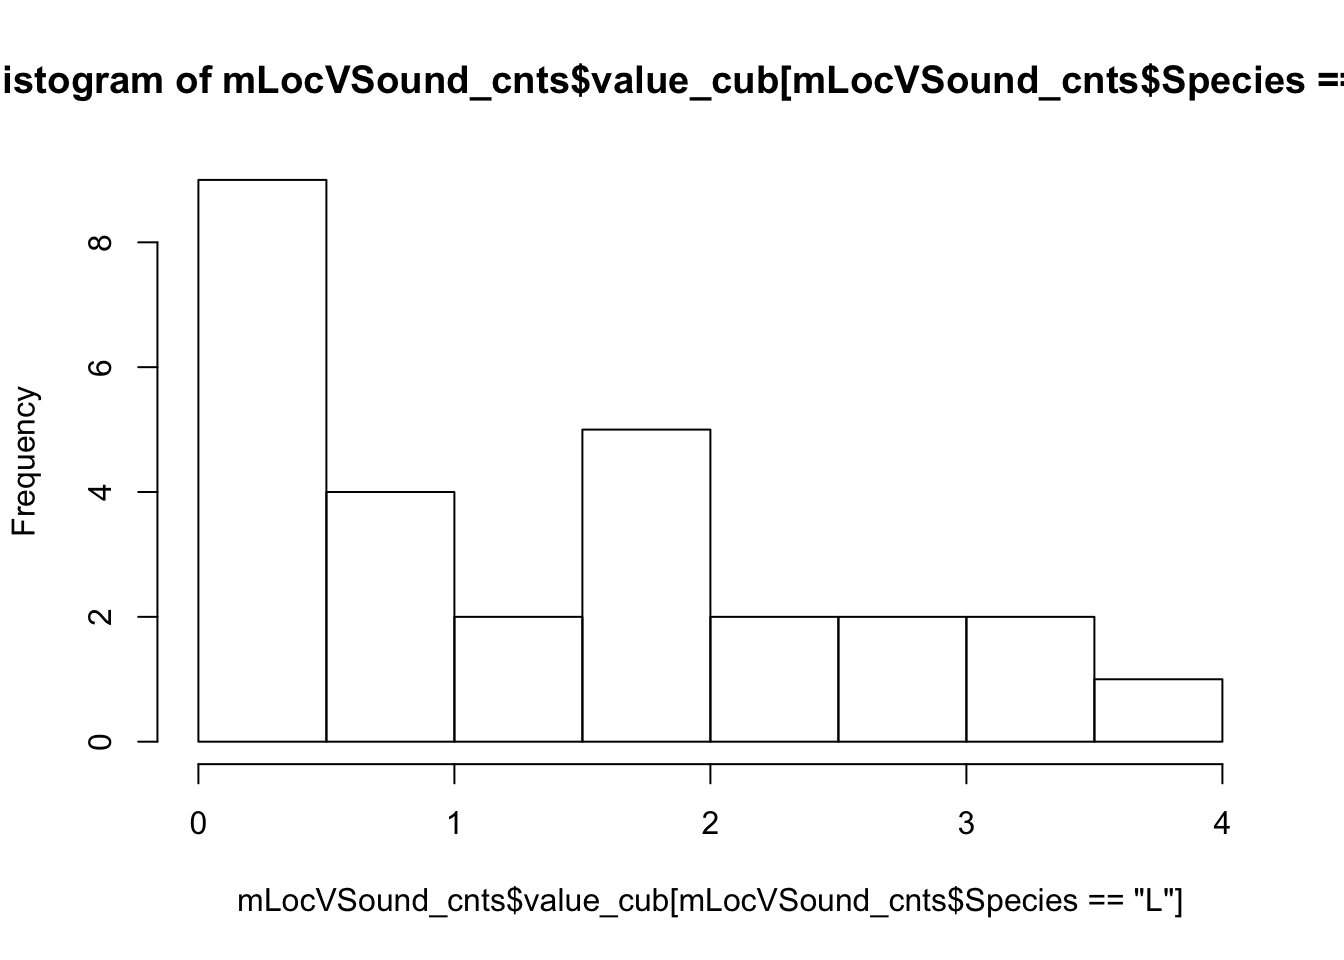
\includegraphics{Sensory_learning_files/figure-latex/unnamed-chunk-17-13.pdf}

\begin{Shaded}
\begin{Highlighting}[]
\KeywordTok{hist}\NormalTok{(mLocVSound_cnts$value_log[mLocVSound_cnts$Species==}\StringTok{"L"}\NormalTok{], }\DataTypeTok{breaks=}\DecValTok{8}\NormalTok{)}
\end{Highlighting}
\end{Shaded}

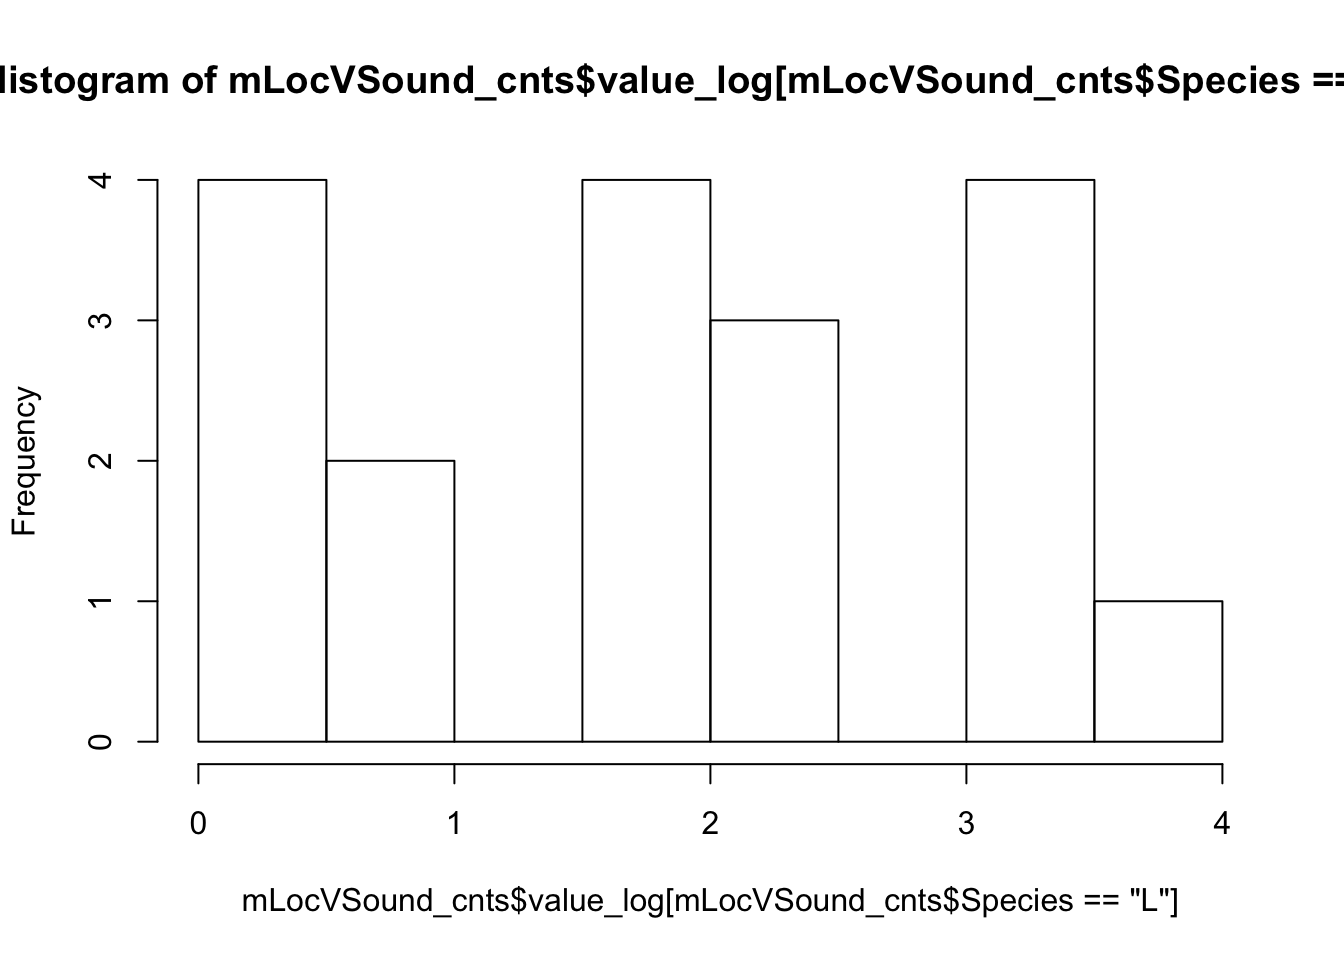
\includegraphics{Sensory_learning_files/figure-latex/unnamed-chunk-17-14.pdf}

\begin{Shaded}
\begin{Highlighting}[]
\KeywordTok{str}\NormalTok{(mLocVSound_cnts)}
\end{Highlighting}
\end{Shaded}

\begin{verbatim}
## 'data.frame':    63 obs. of  7 variables:
##  $ Bat.ID    : Factor w/ 22 levels "A-C095","B-Butt",..: 1 9 17 2 7 3 19 4 15 21 ...
##  $ Species   : Factor w/ 2 levels "AJ","L": 1 1 1 2 2 1 2 2 1 2 ...
##  $ variable  : Factor w/ 3 levels "visits_loc","visits_sound",..: 1 1 1 1 1 1 1 1 1 1 ...
##  $ value     : int  11 6 13 5 22 0 23 9 16 43 ...
##  $ value_sqrt: num  3.32 2.45 3.61 2.24 4.69 ...
##  $ value_cub : num  2.22 1.82 2.35 1.71 2.8 ...
##  $ value_log : num  2.4 1.79 2.56 1.61 3.09 ...
\end{verbatim}

\begin{Shaded}
\begin{Highlighting}[]
\KeywordTok{table}\NormalTok{(mLocVSound_cnts$value)}
\end{Highlighting}
\end{Shaded}

\begin{verbatim}
## 
##  0  1  2  3  4  5  6  7  8  9 10 11 12 13 15 16 18 21 22 23 31 33 43 
## 16  8  2  1  1  5  5  3  3  4  1  2  2  1  1  1  1  1  1  1  1  1  1
\end{verbatim}

\begin{Shaded}
\begin{Highlighting}[]
\KeywordTok{sum}\NormalTok{(mLocVSound_cnts$value ==}\StringTok{ }\DecValTok{0}\NormalTok{)}
\end{Highlighting}
\end{Shaded}

\begin{verbatim}
## [1] 16
\end{verbatim}

\begin{Shaded}
\begin{Highlighting}[]
\NormalTok{##View(mLocVSound_cnts)}
\end{Highlighting}
\end{Shaded}

Probably best to use count data with ANOVA, proportions may be real, so
use the cube transformation \#\# Anova with transformed count data, type
2

\begin{Shaded}
\begin{Highlighting}[]
\KeywordTok{library}\NormalTok{(car)}
\end{Highlighting}
\end{Shaded}

\begin{verbatim}
## Loading required package: carData
\end{verbatim}

\begin{verbatim}
## 
## Attaching package: 'car'
\end{verbatim}

\begin{verbatim}
## The following object is masked from 'package:boot':
## 
##     logit
\end{verbatim}

\begin{verbatim}
## The following object is masked from 'package:FSA':
## 
##     bootCase
\end{verbatim}

\begin{verbatim}
## The following object is masked from 'package:dplyr':
## 
##     recode
\end{verbatim}

\begin{Shaded}
\begin{Highlighting}[]
\NormalTok{anova_LvS <-}\StringTok{ }\KeywordTok{aov}\NormalTok{(value_cub ~}\StringTok{ }\NormalTok{Species*variable, }\DataTypeTok{data=}\NormalTok{mLocVSound_cnts)}
\NormalTok{anova_LvS}
\end{Highlighting}
\end{Shaded}

\begin{verbatim}
## Call:
##    aov(formula = value_cub ~ Species * variable, data = mLocVSound_cnts)
## 
## Terms:
##                  Species variable Species:variable Residuals
## Sum of Squares   0.79690 17.12332          3.29159  41.39585
## Deg. of Freedom        1        2                2        57
## 
## Residual standard error: 0.852199
## Estimated effects may be unbalanced
\end{verbatim}

\begin{Shaded}
\begin{Highlighting}[]
\KeywordTok{Anova}\NormalTok{(anova_LvS, }\DataTypeTok{type =} \DecValTok{2}\NormalTok{)}
\end{Highlighting}
\end{Shaded}

\begin{verbatim}
## Anova Table (Type II tests)
## 
## Response: value_cub
##                  Sum Sq Df F value    Pr(>F)    
## Species           0.797  1  1.0973    0.2993    
## variable         17.123  2 11.7890 5.191e-05 ***
## Species:variable  3.292  2  2.2662    0.1130    
## Residuals        41.396 57                      
## ---
## Signif. codes:  0 '***' 0.001 '**' 0.01 '*' 0.05 '.' 0.1 ' ' 1
\end{verbatim}

No obvious effect of species, only the effect of the treatments. I know
this isn't a really nice way to do this, but not sure how else to do it.

\subsection{confidence intervals and
bootstrapping}\label{confidence-intervals-and-bootstrapping}

\begin{Shaded}
\begin{Highlighting}[]
\NormalTok{## Could get the mean proportion of visits to cues from each of the species. bootstrap the mean proportion, then compare the 95% confidence intervals for each mean }
\NormalTok{############CODE FROM BASTI#################################################}

\CommentTok{#X will be the vector of proportions or rates or counts for one treatment in a species. It will calculate 5000 means based on re-sampling your data and then calculate the confidence intervals from that mean-distribution. }

\CommentTok{#The function spits out a vector of three values, the lower CI, mean, and upper CI.}

\CommentTok{#This is the function used for it:}
\CommentTok{#https://www.rdocumentation.org/packages/boot/versions/1.3-20/topics/boot.ci}
\NormalTok{###########################################################################}

\CommentTok{#mean function}
\NormalTok{mean.w <-}\StringTok{ }\NormalTok{function(x,w) }\KeywordTok{sum}\NormalTok{(x*w) }\CommentTok{# calculates a mean}

\CommentTok{#bootstrapped confidence intervals function}
\NormalTok{boot_ci <-}\StringTok{ }\NormalTok{function(x)\{}
    \NormalTok{mean <-}\StringTok{ }\KeywordTok{mean}\NormalTok{(x)}
    \NormalTok{low <-}\StringTok{ }\KeywordTok{boot.ci}\NormalTok{(}\KeywordTok{boot}\NormalTok{(}\DataTypeTok{data=}\NormalTok{x, }\DataTypeTok{statistic=}\NormalTok{mean.w, }\DataTypeTok{R=}\DecValTok{5000}\NormalTok{, }\DataTypeTok{stype=}\StringTok{"w"}\NormalTok{), }\DataTypeTok{type=}\StringTok{"basic"}\NormalTok{)$basic[}\DecValTok{1}\NormalTok{,}\DecValTok{4}\NormalTok{]}
    \NormalTok{high <-}\StringTok{ }\KeywordTok{boot.ci}\NormalTok{(}\KeywordTok{boot}\NormalTok{(}\DataTypeTok{data=}\NormalTok{x, }\DataTypeTok{statistic=}\NormalTok{mean.w, }\DataTypeTok{R=}\DecValTok{5000}\NormalTok{, }\DataTypeTok{stype=}\StringTok{"w"}\NormalTok{), }\DataTypeTok{type=}\StringTok{"basic"}\NormalTok{)$basic[}\DecValTok{1}\NormalTok{,}\DecValTok{5}\NormalTok{]}
    \KeywordTok{c}\NormalTok{(low,mean,high)\} }\CommentTok{# bootstraps the confidence intervals}



\NormalTok{## get rid of NAs in data using complete.cases}
\NormalTok{mLocVSound_na<-mLocVSound[}\KeywordTok{complete.cases}\NormalTok{(mLocVSound[ ,}\DecValTok{4}\NormalTok{:}\DecValTok{6}\NormalTok{]), ] }\CommentTok{#removes NA rows in value columns 4:6, this might now make sense if I change the number of columns}

\CommentTok{#New database without NAs in the selected columns}
\NormalTok{LocVSound_AJ_L_na <-}\StringTok{ }\NormalTok{LocVSound_AJ_L[}\KeywordTok{complete.cases}\NormalTok{(LocVSound_AJ_L[ ,}\KeywordTok{c}\NormalTok{(}\StringTok{"visits_loc"}\NormalTok{, }\StringTok{"visits_sound"}\NormalTok{,  }\StringTok{"visits_neither"}\NormalTok{, }\StringTok{"pct_visits_loc"}\NormalTok{, }\StringTok{"pct_visits_sound"}\NormalTok{, }\StringTok{"pct_visits_neither"}\NormalTok{)]), ]}

\CommentTok{#The CI's for loc v Sound, percentages}
\KeywordTok{set.seed}\NormalTok{(}\DecValTok{1}\NormalTok{)}
\NormalTok{LvS_pct_CI <-}\StringTok{ }\KeywordTok{do.call}\NormalTok{(data.frame,}\KeywordTok{aggregate}\NormalTok{(value ~}\StringTok{ }\NormalTok{Species +}\StringTok{ }\NormalTok{variable , boot_ci, }\DataTypeTok{data =} \NormalTok{mLocVSound_na)) }\CommentTok{#This applies the bootstrap accross species and treatment variables, and do.call puts the data.frame in the right format}
\KeywordTok{colnames}\NormalTok{(LvS_pct_CI) <-}\StringTok{ }\KeywordTok{c}\NormalTok{(}\StringTok{"Species"}\NormalTok{, }\StringTok{"variable"}\NormalTok{, }\StringTok{"low"}\NormalTok{, }\StringTok{"mean"}\NormalTok{, }\StringTok{"high"}\NormalTok{)}

\CommentTok{# The CIs for Loc V Sound, counts}
\NormalTok{LvS_count_CI <-}\StringTok{ }\KeywordTok{do.call}\NormalTok{(data.frame, }\KeywordTok{aggregate}\NormalTok{(visits_counts ~}\StringTok{ }\NormalTok{Species +}\StringTok{ }\NormalTok{variable , boot_ci, }\DataTypeTok{data =} \NormalTok{mLocVSound_na))}
\NormalTok{LvS_count_CI}
\end{Highlighting}
\end{Shaded}

\begin{verbatim}
##   Species           variable visits_counts.V1 visits_counts.V2
## 1      AJ     pct_visits_loc        8.0909091        10.909091
## 2       L     pct_visits_loc        9.4472313        18.777778
## 3      AJ   pct_visits_sound        1.4545455         4.545455
## 4       L   pct_visits_sound        0.2222222         2.666667
## 5      AJ pct_visits_neither        3.0909091         6.090909
## 6       L pct_visits_neither        0.1111111         1.777778
##   visits_counts.V3
## 1        13.363636
## 2        28.111111
## 3         7.181818
## 4         5.000000
## 5         8.818182
## 6         3.111111
\end{verbatim}

\begin{Shaded}
\begin{Highlighting}[]
\KeywordTok{colnames}\NormalTok{(LvS_count_CI) <-}\StringTok{ }\KeywordTok{c}\NormalTok{(}\StringTok{"Species"}\NormalTok{, }\StringTok{"variable"}\NormalTok{, }\StringTok{"low"}\NormalTok{, }\StringTok{"mean"}\NormalTok{, }\StringTok{"high"}\NormalTok{)}
\end{Highlighting}
\end{Shaded}

\subsection{Plotting}\label{plotting}

\subsection{plotting confidence intervals for pct and \% visits to
platforms,
LvS}\label{plotting-confidence-intervals-for-pct-and-visits-to-platforms-lvs}

\begin{Shaded}
\begin{Highlighting}[]
\CommentTok{#LvS_pct_CI$Species <- factor(LvS_pct_CI$Species, levels=c("AJ", "L"), labels = c("A. jamaicensis", "L. silvicolum")) #need to do this for plot legends to say full name}

\CommentTok{#LvS_count_CI$Species <- factor(LvS_count_CI$Species, levels=c("AJ", "L"), labels = c("A. jamaicensis", "L. silvicolum"))}


\NormalTok{pd =}\StringTok{ }\KeywordTok{position_dodge}\NormalTok{(}\FloatTok{0.5}\NormalTok{) }\CommentTok{# move bars .05 to the left and right}

\CommentTok{#proportion plot}
\NormalTok{LvS_pct_CI_p <-}\StringTok{ }\KeywordTok{ggplot}\NormalTok{(}\DataTypeTok{data =} \NormalTok{LvS_pct_CI, }\KeywordTok{aes}\NormalTok{(}\DataTypeTok{x=}\NormalTok{variable, }\DataTypeTok{y =} \NormalTok{mean, }\DataTypeTok{colour =} \NormalTok{Species))}
\NormalTok{LvS_pct_CI_p <-}\StringTok{ }\NormalTok{LvS_pct_CI_p +}\StringTok{ }\KeywordTok{geom_errorbar}\NormalTok{(}\KeywordTok{aes}\NormalTok{(}\DataTypeTok{ymin =} \NormalTok{low, }\DataTypeTok{ymax =} \NormalTok{high), }\DataTypeTok{width =}\NormalTok{.}\DecValTok{1}\NormalTok{, }\DataTypeTok{position =} \NormalTok{pd)}
\NormalTok{LvS_pct_CI_p <-}\StringTok{ }\NormalTok{LvS_pct_CI_p +}\StringTok{ }\KeywordTok{geom_point}\NormalTok{( }\DataTypeTok{position =} \NormalTok{pd, }\DataTypeTok{shape=}\DecValTok{18}\NormalTok{, }\DataTypeTok{size =} \DecValTok{3}\NormalTok{)}
\NormalTok{LvS_pct_CI_p <-}\StringTok{ }\NormalTok{LvS_pct_CI_p +}\StringTok{ }\KeywordTok{theme}\NormalTok{(}\DataTypeTok{panel.grid.major =} \KeywordTok{element_blank}\NormalTok{(), }\DataTypeTok{panel.grid.minor =} \KeywordTok{element_blank}\NormalTok{(),}
\DataTypeTok{panel.background =} \KeywordTok{element_blank}\NormalTok{(), }\DataTypeTok{axis.line =} \KeywordTok{element_line}\NormalTok{(}\DataTypeTok{colour =} \StringTok{"black"}\NormalTok{), }\DataTypeTok{axis.text =} \KeywordTok{element_text}\NormalTok{(}\DataTypeTok{colour =} \StringTok{"black"}\NormalTok{), }\DataTypeTok{legend.text =} \KeywordTok{element_text}\NormalTok{(}\DataTypeTok{face =} \StringTok{"italic"}\NormalTok{))  }\CommentTok{#gets rid of background, makes legend italic}

\NormalTok{LvS_pct_CI_p <-}\StringTok{ }\NormalTok{LvS_pct_CI_p +}\StringTok{ }\KeywordTok{scale_x_discrete}\NormalTok{(}\DataTypeTok{labels=}\KeywordTok{c}\NormalTok{(}\StringTok{"pct_visits_loc"} \NormalTok{=}\StringTok{ "Location"}\NormalTok{, }\StringTok{"pct_visits_sound"} \NormalTok{=}\StringTok{ "Sound"}\NormalTok{,}
                              \StringTok{"pct_visits_neither"} \NormalTok{=}\StringTok{ "Neither"}\NormalTok{))  }\CommentTok{# Relabelling X axis}
\NormalTok{LvS_pct_CI_p <-}\StringTok{ }\NormalTok{LvS_pct_CI_p +}\StringTok{ }\KeywordTok{xlab}\NormalTok{(}\StringTok{"Cues"}\NormalTok{)}
\NormalTok{LvS_pct_CI_p <-}\StringTok{ }\NormalTok{LvS_pct_CI_p +}\StringTok{ }\KeywordTok{ylab}\NormalTok{(}\StringTok{"Mean proportion of visits"}\NormalTok{)}
\NormalTok{LvS_pct_CI_p <-}\StringTok{ }\NormalTok{LvS_pct_CI_p +}\StringTok{ }\KeywordTok{scale_color_manual}\NormalTok{(}\DataTypeTok{values =} \KeywordTok{c}\NormalTok{(Lo, Art), }\DataTypeTok{labels =} \KeywordTok{c}\NormalTok{(}\StringTok{"AJ"} \NormalTok{=}\StringTok{ "A. jamaicensis"}\NormalTok{, }\StringTok{"L"} \NormalTok{=}\StringTok{ "L. silvicolum"}\NormalTok{))}


\NormalTok{LvS_pct_CI_p                    }
\end{Highlighting}
\end{Shaded}

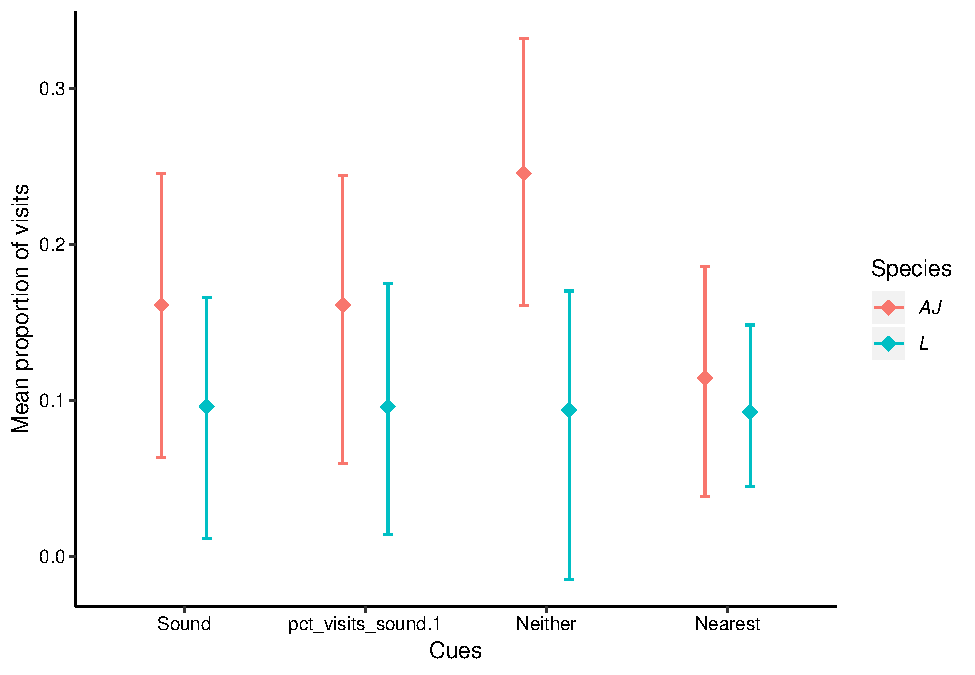
\includegraphics{Sensory_learning_files/figure-latex/unnamed-chunk-20-1.pdf}

\begin{Shaded}
\begin{Highlighting}[]
\CommentTok{#ggsave("LvS_pct_CI_p.png" )}

\CommentTok{#count plot}
\NormalTok{LvS_count_CI_p <-}\StringTok{ }\KeywordTok{ggplot}\NormalTok{(}\DataTypeTok{data =} \NormalTok{LvS_count_CI, }\KeywordTok{aes}\NormalTok{(}\DataTypeTok{x=}\NormalTok{variable, }\DataTypeTok{y =} \NormalTok{mean, }\DataTypeTok{colour =} \NormalTok{Species))}
\NormalTok{LvS_count_CI_p <-}\StringTok{ }\NormalTok{LvS_count_CI_p +}\StringTok{ }\KeywordTok{geom_errorbar}\NormalTok{(}\KeywordTok{aes}\NormalTok{(}\DataTypeTok{ymin =} \NormalTok{low, }\DataTypeTok{ymax =} \NormalTok{high), }\DataTypeTok{width =}\NormalTok{.}\DecValTok{1}\NormalTok{, }\DataTypeTok{position =} \NormalTok{pd)}
\NormalTok{LvS_count_CI_p <-}\StringTok{ }\NormalTok{LvS_count_CI_p +}\StringTok{ }\KeywordTok{geom_point}\NormalTok{( }\DataTypeTok{position =} \NormalTok{pd, }\DataTypeTok{shape=}\DecValTok{18}\NormalTok{, }\DataTypeTok{size =} \DecValTok{3}\NormalTok{)}
\NormalTok{LvS_count_CI_p <-}\StringTok{ }\NormalTok{LvS_count_CI_p +}\StringTok{ }\KeywordTok{theme}\NormalTok{(}\DataTypeTok{panel.grid.major =} \KeywordTok{element_blank}\NormalTok{(), }\DataTypeTok{panel.grid.minor =} \KeywordTok{element_blank}\NormalTok{(),}
\DataTypeTok{panel.background =} \KeywordTok{element_blank}\NormalTok{(), }\DataTypeTok{axis.line =} \KeywordTok{element_line}\NormalTok{(}\DataTypeTok{colour =} \StringTok{"black"}\NormalTok{), }\DataTypeTok{axis.text =} \KeywordTok{element_text}\NormalTok{(}\DataTypeTok{colour =} \StringTok{"black"}\NormalTok{), }\DataTypeTok{legend.text =} \KeywordTok{element_text}\NormalTok{(}\DataTypeTok{face =} \StringTok{"italic"}\NormalTok{))  }\CommentTok{#gets rid of background, makes legend italic}

\NormalTok{LvS_count_CI_p <-}\StringTok{ }\NormalTok{LvS_count_CI_p +}\StringTok{ }\KeywordTok{scale_x_discrete}\NormalTok{(}\DataTypeTok{labels=}\KeywordTok{c}\NormalTok{(}\StringTok{"pct_visits_loc"} \NormalTok{=}\StringTok{ "Location"}\NormalTok{, }\StringTok{"pct_visits_sound"} \NormalTok{=}\StringTok{ "Sound"}\NormalTok{,}
                              \StringTok{"pct_visits_neither"} \NormalTok{=}\StringTok{ "Neither"}\NormalTok{))  }\CommentTok{# Relabelling X axis}
\NormalTok{LvS_count_CI_p <-}\StringTok{ }\NormalTok{LvS_count_CI_p +}\StringTok{ }\KeywordTok{xlab}\NormalTok{(}\StringTok{"Cues"}\NormalTok{)}
\NormalTok{LvS_count_CI_p <-}\StringTok{ }\NormalTok{LvS_count_CI_p +}\StringTok{ }\KeywordTok{ylab}\NormalTok{(}\StringTok{"Mean number of visits"}\NormalTok{)}
\NormalTok{LvS_count_CI_p <-}\StringTok{ }\NormalTok{LvS_count_CI_p +}\StringTok{ }\KeywordTok{scale_color_manual}\NormalTok{(}\DataTypeTok{values =} \KeywordTok{c}\NormalTok{(Lo, Art), }\DataTypeTok{labels =} \KeywordTok{c}\NormalTok{(}\StringTok{"AJ"} \NormalTok{=}\StringTok{ "A. jamaicensis"}\NormalTok{, }\StringTok{"L"} \NormalTok{=}\StringTok{ "L. silvicolum"}\NormalTok{))}

\NormalTok{LvS_count_CI_p }
\end{Highlighting}
\end{Shaded}

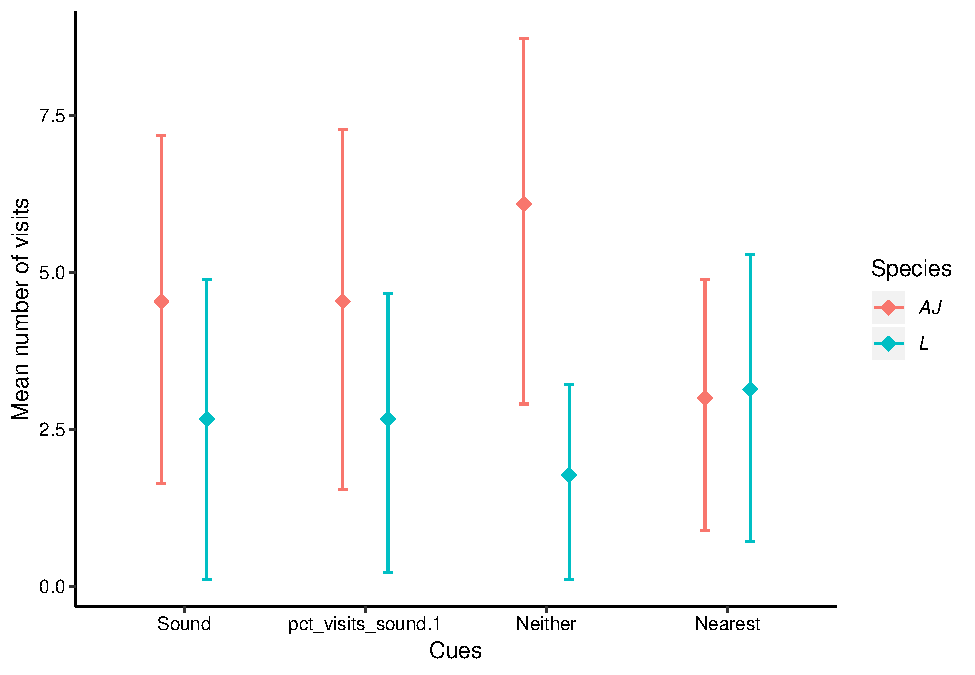
\includegraphics{Sensory_learning_files/figure-latex/unnamed-chunk-20-2.pdf}

\begin{Shaded}
\begin{Highlighting}[]
\CommentTok{#ggsave("LvS_count_CI_p.png" )}
\end{Highlighting}
\end{Shaded}

\paragraph{Plotting \% of visits to the different platforms,
LvS}\label{plotting-of-visits-to-the-different-platforms-lvs}

\begin{Shaded}
\begin{Highlighting}[]
\NormalTok{LocVSound_bar <-}\StringTok{ }\KeywordTok{ggplot}\NormalTok{(}\DataTypeTok{data =}\NormalTok{mLocVSound, }\KeywordTok{aes}\NormalTok{(}\DataTypeTok{x =} \NormalTok{variable, }\DataTypeTok{y =} \NormalTok{value))}
\NormalTok{LocVSound_bar <-}\StringTok{ }\NormalTok{LocVSound_bar +}\StringTok{ }\KeywordTok{geom_boxplot}\NormalTok{(}\KeywordTok{aes}\NormalTok{(}\DataTypeTok{fill=}\NormalTok{Species))}
\NormalTok{LocVSound_bar <-}\StringTok{ }\NormalTok{LocVSound_bar +}\StringTok{ }\KeywordTok{geom_point}\NormalTok{(}\DataTypeTok{position=}\KeywordTok{position_dodge}\NormalTok{(}\DataTypeTok{width=}\FloatTok{0.75}\NormalTok{), }\KeywordTok{aes}\NormalTok{(}\DataTypeTok{group=}\NormalTok{Species), }\DataTypeTok{alpha =} \DecValTok{1}\NormalTok{/}\DecValTok{4}\NormalTok{) }\CommentTok{#makes points semi-transparent}
\NormalTok{LocVSound_bar <-}\StringTok{ }\NormalTok{LocVSound_bar +}\StringTok{ }\KeywordTok{theme}\NormalTok{(}\DataTypeTok{panel.grid.major =} \KeywordTok{element_blank}\NormalTok{(), }\DataTypeTok{panel.grid.minor =} \KeywordTok{element_blank}\NormalTok{(),}
\DataTypeTok{panel.background =} \KeywordTok{element_blank}\NormalTok{(), }\DataTypeTok{axis.line =} \KeywordTok{element_line}\NormalTok{(}\DataTypeTok{colour =} \StringTok{"black"}\NormalTok{), }\DataTypeTok{axis.text =} \KeywordTok{element_text}\NormalTok{(}\DataTypeTok{colour =} \StringTok{"black"}\NormalTok{), }\DataTypeTok{legend.text =} \KeywordTok{element_text}\NormalTok{(}\DataTypeTok{face =} \StringTok{"italic"}\NormalTok{))  }\CommentTok{#gets rid of background, makes legend italic}
\NormalTok{LocVSound_bar <-}\StringTok{ }\NormalTok{LocVSound_bar +}\StringTok{ }\KeywordTok{xlab}\NormalTok{(}\StringTok{"Cues"}\NormalTok{)}
\NormalTok{LocVSound_bar <-}\StringTok{ }\NormalTok{LocVSound_bar +}\StringTok{ }\KeywordTok{ylab}\NormalTok{(}\StringTok{"Proportion of total visits"}\NormalTok{)}
\NormalTok{LocVSound_bar <-}\StringTok{ }\NormalTok{LocVSound_bar +}\StringTok{ }\KeywordTok{scale_x_discrete}\NormalTok{(}\DataTypeTok{labels=}\KeywordTok{c}\NormalTok{(}\StringTok{"pct_visits_loc"} \NormalTok{=}\StringTok{ "Location"}\NormalTok{, }\StringTok{"pct_visits_sound"} \NormalTok{=}\StringTok{ "Sound"}\NormalTok{,}
                              \StringTok{"pct_visits_neither"} \NormalTok{=}\StringTok{ "Neither"} \NormalTok{))  }\CommentTok{# Relabelling X axis}
\CommentTok{#LocVSound_bar <- LocVSound_bar + scale_fill_discrete(labels = c("AJ" = "A. jamaicensis", "L" = "L. silvicolum"))}
\NormalTok{LocVSound_bar <-}\StringTok{ }\NormalTok{LocVSound_bar +}\StringTok{ }\KeywordTok{scale_fill_manual}\NormalTok{(}\DataTypeTok{values =} \KeywordTok{c}\NormalTok{(Lo, Art), }\DataTypeTok{labels =} \KeywordTok{c}\NormalTok{(}\StringTok{"AJ"} \NormalTok{=}\StringTok{ "A. jamaicensis"}\NormalTok{, }\StringTok{"L"} \NormalTok{=}\StringTok{ "L. silvicolum"}\NormalTok{))}
\NormalTok{LocVSound_bar}
\end{Highlighting}
\end{Shaded}

\begin{verbatim}
## Warning: Removed 3 rows containing non-finite values (stat_boxplot).
\end{verbatim}

\begin{verbatim}
## Warning: Removed 3 rows containing missing values (geom_point).
\end{verbatim}

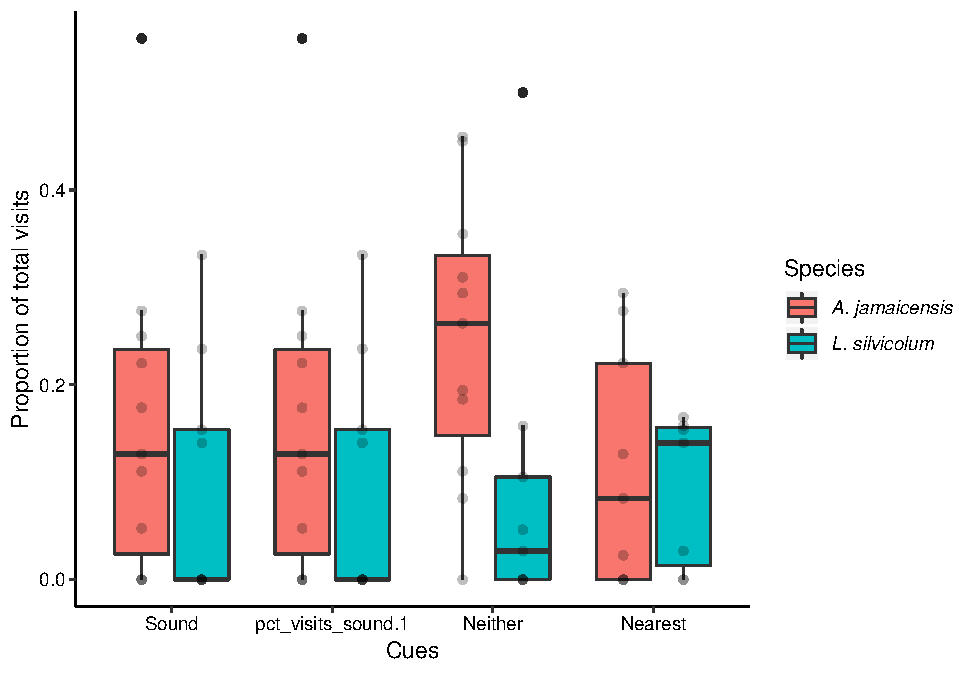
\includegraphics{Sensory_learning_files/figure-latex/unnamed-chunk-21-1.pdf}

\begin{Shaded}
\begin{Highlighting}[]
\CommentTok{#ggsave("LocVSound_pcts.png")}
\end{Highlighting}
\end{Shaded}

\paragraph{Plotting absolute number of visits to the different
platforms}\label{plotting-absolute-number-of-visits-to-the-different-platforms}

\begin{Shaded}
\begin{Highlighting}[]
\NormalTok{LocVSound_bar_cnts <-}\StringTok{ }\KeywordTok{ggplot}\NormalTok{(}\DataTypeTok{data =}\NormalTok{mLocVSound_cnts, }\KeywordTok{aes}\NormalTok{(}\DataTypeTok{x =} \NormalTok{variable, }\DataTypeTok{y =} \NormalTok{value))}
\NormalTok{LocVSound_bar_cnts <-}\StringTok{ }\NormalTok{LocVSound_bar_cnts +}\StringTok{ }\KeywordTok{geom_boxplot}\NormalTok{(}\KeywordTok{aes}\NormalTok{(}\DataTypeTok{fill=}\NormalTok{Species))}
\NormalTok{LocVSound_bar_cnts <-}\StringTok{ }\NormalTok{LocVSound_bar_cnts +}\StringTok{ }\KeywordTok{geom_point}\NormalTok{(}\DataTypeTok{position=}\KeywordTok{position_dodge}\NormalTok{(}\DataTypeTok{width=}\FloatTok{0.75}\NormalTok{), }\KeywordTok{aes}\NormalTok{(}\DataTypeTok{group=}\NormalTok{Species), }\DataTypeTok{alpha =} \DecValTok{1}\NormalTok{/}\DecValTok{4}\NormalTok{) }\CommentTok{#makes points semi-transparent}
\NormalTok{LocVSound_bar_cnts <-}\StringTok{ }\NormalTok{LocVSound_bar_cnts +}\StringTok{ }\KeywordTok{theme}\NormalTok{(}\DataTypeTok{panel.grid.major =} \KeywordTok{element_blank}\NormalTok{(), }\DataTypeTok{panel.grid.minor =} \KeywordTok{element_blank}\NormalTok{(),}
\DataTypeTok{panel.background =} \KeywordTok{element_blank}\NormalTok{(), }\DataTypeTok{axis.line =} \KeywordTok{element_line}\NormalTok{(}\DataTypeTok{colour =} \StringTok{"black"}\NormalTok{), }\DataTypeTok{axis.text =} \KeywordTok{element_text}\NormalTok{(}\DataTypeTok{colour =} \StringTok{"black"}\NormalTok{), }\DataTypeTok{legend.text =} \KeywordTok{element_text}\NormalTok{(}\DataTypeTok{face =} \StringTok{"italic"}\NormalTok{))  }\CommentTok{#gets rid of background, makes legend italic}
\NormalTok{LocVSound_bar_cnts <-}\StringTok{ }\NormalTok{LocVSound_bar_cnts +}\StringTok{ }\KeywordTok{xlab}\NormalTok{(}\StringTok{"Cues"}\NormalTok{)}
\NormalTok{LocVSound_bar_cnts <-}\StringTok{ }\NormalTok{LocVSound_bar_cnts +}\StringTok{ }\KeywordTok{ylab}\NormalTok{(}\StringTok{"Number of visits"}\NormalTok{)}
\NormalTok{LocVSound_bar_cnts <-}\StringTok{ }\NormalTok{LocVSound_bar_cnts +}\StringTok{ }\KeywordTok{scale_x_discrete}\NormalTok{(}\DataTypeTok{labels=}\KeywordTok{c}\NormalTok{(}\StringTok{"visits_loc"} \NormalTok{=}\StringTok{ "Location"}\NormalTok{, }\StringTok{"visits_sound"} \NormalTok{=}\StringTok{ "Sound"}\NormalTok{,}
                              \StringTok{"visits_neither"} \NormalTok{=}\StringTok{ "Neither"} \NormalTok{))  }\CommentTok{# Relabelling X axis}
\NormalTok{LocVSound_bar_cnts <-}\StringTok{ }\NormalTok{LocVSound_bar_cnts +}\StringTok{ }\KeywordTok{scale_fill_manual}\NormalTok{(}\DataTypeTok{values =} \KeywordTok{c}\NormalTok{(Lo, Art), }\DataTypeTok{labels =} \KeywordTok{c}\NormalTok{(}\StringTok{"AJ"} \NormalTok{=}\StringTok{ "A. jamaicensis"}\NormalTok{, }\StringTok{"L"} \NormalTok{=}\StringTok{ "L. silvicolum"}\NormalTok{))}
\NormalTok{LocVSound_bar_cnts}
\end{Highlighting}
\end{Shaded}

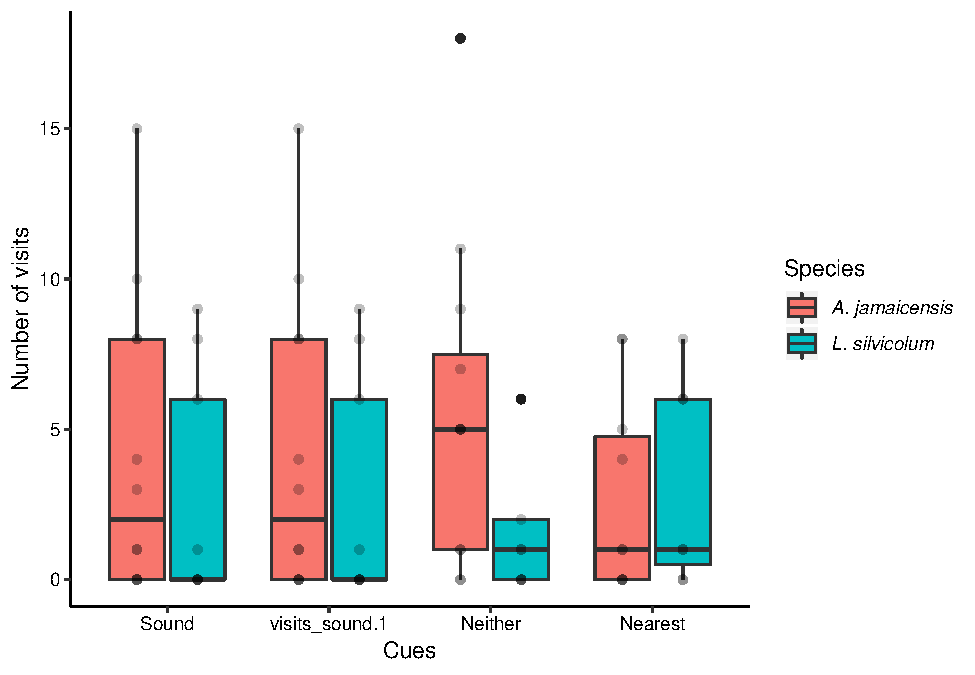
\includegraphics{Sensory_learning_files/figure-latex/unnamed-chunk-22-1.pdf}

\begin{Shaded}
\begin{Highlighting}[]
\CommentTok{#ggsave("LocVSound_cnts.png")}
\end{Highlighting}
\end{Shaded}

\section{rm(LocVSound\_bar)}\label{rmlocvsound_bar}

\subsection{First choices/ visits by
species}\label{first-choices-visits-by-species}

\subsection{Make new data frame with summary data for first
visits}\label{make-new-data-frame-with-summary-data-for-first-visits}

\begin{Shaded}
\begin{Highlighting}[]
\KeywordTok{head}\NormalTok{(first_choices)}
\end{Highlighting}
\end{Shaded}

\begin{verbatim}
## # A tibble: 6 x 11
##   `Bat ID` Scorer Date  Time  Species Test  Rewarded_1 Rewarded_2
##   <chr>    <chr>  <chr> <chr> <chr>   <chr> <chr>      <chr>     
## 1 A-C095   unkno~ 4/1/~ 1     AJ      LocV~ 4,2        epsilon   
## 2 D-C0B6   unkno~ 4/2/~ 23:45 AJ      LocV~ 4,2        epsilon   
## 3 K-C091   May    4/30~ 21:47 AJ      LocV~ 3,3        feta      
## 4 B-Butt   Dylan  7/1/~ 21:37 L       LocV~ 3,1        feta      
## 5 C-Newbie Dylan  7/1/~ 19:12 L       LocV~ 3,2        feta      
## 6 B-C09E   Dylan  4/5/~ 19:41 AJ      LocV~ 4,2        epsilon   
## # ... with 3 more variables: first_hover <chr>, first_land <chr>,
## #   first_visit <fct>
\end{verbatim}

\begin{Shaded}
\begin{Highlighting}[]
\NormalTok{fc_LocVSound<-}\StringTok{ }\NormalTok{first_choices[first_choices$Test==}\StringTok{"LocVSound"} \NormalTok{&}\StringTok{ }\NormalTok{first_choices$first_visit!=}\StringTok{ "nearest"}\NormalTok{,] }\CommentTok{#pulling out Loc V Sound and cutting nearests}
\KeywordTok{head}\NormalTok{(fc_LocVSound)}
\end{Highlighting}
\end{Shaded}

\begin{verbatim}
## # A tibble: 6 x 11
##   `Bat ID` Scorer Date  Time  Species Test  Rewarded_1 Rewarded_2
##   <chr>    <chr>  <chr> <chr> <chr>   <chr> <chr>      <chr>     
## 1 A-C095   unkno~ 4/1/~ 1     AJ      LocV~ 4,2        epsilon   
## 2 D-C0B6   unkno~ 4/2/~ 23:45 AJ      LocV~ 4,2        epsilon   
## 3 K-C091   May    4/30~ 21:47 AJ      LocV~ 3,3        feta      
## 4 B-Butt   Dylan  7/1/~ 21:37 L       LocV~ 3,1        feta      
## 5 C-Newbie Dylan  7/1/~ 19:12 L       LocV~ 3,2        feta      
## 6 <NA>     <NA>   <NA>  <NA>  <NA>    <NA>  <NA>       <NA>      
## # ... with 3 more variables: first_hover <chr>, first_land <chr>,
## #   first_visit <fct>
\end{verbatim}

\begin{Shaded}
\begin{Highlighting}[]
\NormalTok{fc_LocVSound$first_visit <-}\StringTok{ }\KeywordTok{factor}\NormalTok{(fc_LocVSound$first_visit, }\DataTypeTok{levels =} \KeywordTok{c}\NormalTok{(}\StringTok{"location"}\NormalTok{, }\StringTok{"sound"}\NormalTok{, }\StringTok{"neither"}\NormalTok{))  }\CommentTok{#redo factor order, removes extra levels}

\KeywordTok{unique}\NormalTok{(fc_LocVSound$first_visit)}
\end{Highlighting}
\end{Shaded}

\begin{verbatim}
## [1] location neither  <NA>     sound   
## Levels: location sound neither
\end{verbatim}

\begin{Shaded}
\begin{Highlighting}[]
\CommentTok{# This does the same thing, but makes a new dataframe to do it}
\CommentTok{#summarize occurances}
\NormalTok{first_visits_LvS <-}\StringTok{ }\KeywordTok{as.data.frame}\NormalTok{(}\KeywordTok{table}\NormalTok{(fc_LocVSound$first_visit, fc_LocVSound$Species)) }\CommentTok{#summarized by species into table}



\KeywordTok{names}\NormalTok{(first_visits_LvS)<-}\StringTok{ }\KeywordTok{c}\NormalTok{(}\StringTok{"Cue"}\NormalTok{, }\StringTok{"Species"}\NormalTok{, }\StringTok{"Visits"}\NormalTok{)}
\NormalTok{## For plotting purposes, need to replace 0's with a small number, not meaningful}
 \NormalTok{first_visits_LvS_fp <-}\StringTok{ }\NormalTok{first_visits_LvS }\CommentTok{#first visits for plot}
 \NormalTok{first_visits_LvS_fp[first_visits_LvS_fp ==}\StringTok{ }\DecValTok{0}\NormalTok{] <-}\StringTok{ }\FloatTok{0.03} 
 
 \CommentTok{#reorder factor}
\CommentTok{#first_visits_LvS_fp$Cue<- factor(first_visits_LvS_fp$Cue, levels = c("location", "sound", "neither", "nearest"))}
\CommentTok{#View(first_visits_LvS_fp)}

\NormalTok{first_visits_LvS_wide <-}\StringTok{ }\KeywordTok{dcast}\NormalTok{(first_visits_LvS, Cue~Species ) }\CommentTok{#reshapes into wide format}
\end{Highlighting}
\end{Shaded}

\begin{verbatim}
## Using Visits as value column: use value.var to override.
\end{verbatim}

\begin{Shaded}
\begin{Highlighting}[]
\KeywordTok{head}\NormalTok{(first_visits_LvS_wide)}
\end{Highlighting}
\end{Shaded}

\begin{verbatim}
##        Cue AJ L
## 1 location  9 5
## 2    sound  1 1
## 3  neither  2 3
\end{verbatim}

\subsection{STATS first visit}\label{stats-first-visit}

Did the bats visit the platforms first equally? Did the species visit
differently?

\section{first visits, exact multinomial test:
AJs}\label{first-visits-exact-multinomial-test-ajs}

Did the bats visit the platforms equally? Independent variable: 0
Dependent variable: \# first visits to 3 platforms, compared to random

\begin{Shaded}
\begin{Highlighting}[]
\NormalTok{## MUST CHANGE THESE NUMBERS MANUALLY ##}
\CommentTok{# Did the AJs  visit the three platforms equally?}
\CommentTok{# Use exact multinomial test: categorical data, small sample sizes}

\CommentTok{# AJs are in column #2:}
\NormalTok{observed_LvS_AJ <-}\StringTok{ }\KeywordTok{c}\NormalTok{(first_visits_LvS_wide[first_visits_LvS_wide==}\StringTok{"location"}\NormalTok{, }\DecValTok{2}\NormalTok{], first_visits_LvS_wide[first_visits_LvS_wide==}\StringTok{"neither"}\NormalTok{, }\DecValTok{2}\NormalTok{], first_visits_LvS_wide[first_visits_LvS_wide==}\StringTok{"sound"}\NormalTok{, }\DecValTok{2}\NormalTok{])}
\NormalTok{observed_LvS_AJ    }\CommentTok{#observed number of visits to the three different platforms}
\end{Highlighting}
\end{Shaded}

\begin{verbatim}
## [1] 9 2 1
\end{verbatim}

\begin{Shaded}
\begin{Highlighting}[]
\NormalTok{prob <-}\StringTok{ }\KeywordTok{rep}\NormalTok{(}\FloatTok{0.33}\NormalTok{, }\DecValTok{3}\NormalTok{) }\CommentTok{#expected number of visits if they are all equal}
\NormalTok{prob }
\end{Highlighting}
\end{Shaded}

\begin{verbatim}
## [1] 0.33 0.33 0.33
\end{verbatim}

\begin{Shaded}
\begin{Highlighting}[]
\NormalTok{mult_test_LvS_AJ <-}\StringTok{ }\KeywordTok{multinomial.test}\NormalTok{(observed_LvS_AJ, prob) }\CommentTok{#exact multinomial test}
\end{Highlighting}
\end{Shaded}

\begin{verbatim}
## 
##  Exact Multinomial Test, distance measure: p
## 
##     Events    pObs    p.value
##         91  0.0012     0.0172
\end{verbatim}

\begin{Shaded}
\begin{Highlighting}[]
\NormalTok{mult_test_LvS_AJ }\CommentTok{# p = 0.0172}
\end{Highlighting}
\end{Shaded}

\begin{verbatim}
## $id
## [1] "Exact Multinomial Test"
## 
## $size
## [1] 12
## 
## $groups
## [1] 3
## 
## $stat
## [1] "lowP"
## 
## $allProb
##  [1] 6.520009e-02 5.216007e-02 5.216007e-02 5.216007e-02 5.216007e-02
##  [6] 5.216007e-02 5.216007e-02 3.477338e-02 3.477338e-02 3.477338e-02
## [11] 3.129604e-02 3.129604e-02 3.129604e-02 2.608004e-02 2.608004e-02
## [16] 2.608004e-02 2.608004e-02 2.608004e-02 2.608004e-02 1.490288e-02
## [21] 1.490288e-02 1.490288e-02 1.490288e-02 1.490288e-02 1.490288e-02
## [26] 1.043201e-02 1.043201e-02 1.043201e-02 1.043201e-02 1.043201e-02
## [31] 1.043201e-02 7.451439e-03 7.451439e-03 7.451439e-03 7.451439e-03
## [36] 7.451439e-03 7.451439e-03 5.588579e-03 5.588579e-03 5.588579e-03
## [41] 3.725719e-03 3.725719e-03 3.725719e-03 3.725719e-03 3.725719e-03
## [46] 3.725719e-03 1.738669e-03 1.738669e-03 1.738669e-03 1.490288e-03
## [51] 1.490288e-03 1.490288e-03 1.490288e-03 1.490288e-03 1.490288e-03
## [56] 1.241906e-03 1.241906e-03 1.241906e-03 1.241906e-03 1.241906e-03
## [61] 1.241906e-03 9.314298e-04 9.314298e-04 9.314298e-04 9.314298e-04
## [66] 9.314298e-04 9.314298e-04 4.139688e-04 4.139688e-04 4.139688e-04
## [71] 4.139688e-04 4.139688e-04 4.139688e-04 2.483813e-04 2.483813e-04
## [76] 2.483813e-04 1.241906e-04 1.241906e-04 1.241906e-04 1.241906e-04
## [81] 1.241906e-04 1.241906e-04 2.258012e-05 2.258012e-05 2.258012e-05
## [86] 2.258012e-05 2.258012e-05 2.258012e-05 1.881676e-06 1.881676e-06
## [91] 1.881676e-06
## 
## $ntrial
## NULL
## 
## $p.value
## [1] 0.0172
\end{verbatim}

\begin{Shaded}
\begin{Highlighting}[]
\NormalTok{#####What kind of posthocs? Do A binomial test, with the treatment in question, and the sum of the other treatments, and then do a Boneferroni correction: divide the significance level by the number of comparisons. My significance value is: 0.0167}
\CommentTok{#http://www.biostathandbook.com/exactgof.html}
\NormalTok{observed_LvS_AJ}
\end{Highlighting}
\end{Shaded}

\begin{verbatim}
## [1] 9 2 1
\end{verbatim}

\begin{Shaded}
\begin{Highlighting}[]
\NormalTok{prob2<-}\StringTok{ }\KeywordTok{c}\NormalTok{(.}\DecValTok{33}\NormalTok{, .}\DecValTok{66}\NormalTok{)}

\NormalTok{obs_LvS_AJ_loc<-}\KeywordTok{c}\NormalTok{(}\DecValTok{9}\NormalTok{,}\DecValTok{3}\NormalTok{)}
\NormalTok{obs_LvS_AJ_sound <-}\StringTok{ }\KeywordTok{c}\NormalTok{(}\DecValTok{1}\NormalTok{, }\DecValTok{11}\NormalTok{)}
\NormalTok{obs_LvS_AJ_neither <-}\StringTok{ }\KeywordTok{c}\NormalTok{(}\DecValTok{2}\NormalTok{, }\DecValTok{10}\NormalTok{)}

\CommentTok{#Boneferroni: .0125 significance for posthocs}
 \KeywordTok{multinomial.test}\NormalTok{(obs_LvS_AJ_loc, prob2) }\CommentTok{# p=0.0039 (significance )}
\end{Highlighting}
\end{Shaded}

\begin{verbatim}
## 
##  Exact Multinomial Test, distance measure: p
## 
##     Events    pObs    p.value
##         13  0.0033     0.0039
\end{verbatim}

\begin{Shaded}
\begin{Highlighting}[]
 \KeywordTok{multinomial.test}\NormalTok{(obs_LvS_AJ_sound, prob2) }\CommentTok{#p = 0.0727}
\end{Highlighting}
\end{Shaded}

\begin{verbatim}
## 
##  Exact Multinomial Test, distance measure: p
## 
##     Events    pObs    p.value
##         13  0.0462     0.0727
\end{verbatim}

\begin{Shaded}
\begin{Highlighting}[]
 \KeywordTok{multinomial.test}\NormalTok{(obs_LvS_AJ_neither, prob2) }\CommentTok{# p = 0.3588}
\end{Highlighting}
\end{Shaded}

\begin{verbatim}
## 
##  Exact Multinomial Test, distance measure: p
## 
##     Events    pObs    p.value
##         13  0.1272     0.3588
\end{verbatim}

\begin{Shaded}
\begin{Highlighting}[]
\CommentTok{# Exact multinomial test suggests that This is more visits to Location that expected at random}
\end{Highlighting}
\end{Shaded}

So AJs went to Sound more than the other places

\section{first visits, exact multinomial test:
Lophos}\label{first-visits-exact-multinomial-test-lophos}

\begin{Shaded}
\begin{Highlighting}[]
\NormalTok{## MUST CHANGE THESE NUMBERS MANUALLY ##}
\CommentTok{# Did the Lophos  visit the three platforms equally?}
\CommentTok{# Use exact multinomial test: categorical data, small sample sizes}

\CommentTok{# Ls are in column #2:}
\NormalTok{observed_LvS_L <-}\StringTok{ }\KeywordTok{c}\NormalTok{(first_visits_LvS_wide[first_visits_LvS_wide==}\StringTok{"location"}\NormalTok{, }\DecValTok{3}\NormalTok{], first_visits_LvS_wide[first_visits_LvS_wide==}\StringTok{"neither"}\NormalTok{, }\DecValTok{3}\NormalTok{], first_visits_LvS_wide[first_visits_LvS_wide==}\StringTok{"sound"}\NormalTok{, }\DecValTok{3}\NormalTok{])}
\NormalTok{observed_LvS_L    }\CommentTok{#observed number of visits to the three different platforms}
\end{Highlighting}
\end{Shaded}

\begin{verbatim}
## [1] 5 3 1
\end{verbatim}

\begin{Shaded}
\begin{Highlighting}[]
\NormalTok{prob <-}\StringTok{ }\KeywordTok{rep}\NormalTok{(}\FloatTok{0.33}\NormalTok{, }\DecValTok{3}\NormalTok{) }\CommentTok{#expected number of visits if they are all equal}
\NormalTok{prob }
\end{Highlighting}
\end{Shaded}

\begin{verbatim}
## [1] 0.33 0.33 0.33
\end{verbatim}

\begin{Shaded}
\begin{Highlighting}[]
\NormalTok{mult_test_LvS_L <-}\StringTok{ }\KeywordTok{multinomial.test}\NormalTok{(observed_LvS_L, prob) }\CommentTok{#exact multinomial test}
\end{Highlighting}
\end{Shaded}

\begin{verbatim}
## 
##  Exact Multinomial Test, distance measure: p
## 
##     Events    pObs    p.value
##         55  0.0256     0.3193
\end{verbatim}

\begin{Shaded}
\begin{Highlighting}[]
\NormalTok{mult_test_LvS_L }\CommentTok{# 0.3193}
\end{Highlighting}
\end{Shaded}

\begin{verbatim}
## $id
## [1] "Exact Multinomial Test"
## 
## $size
## [1] 9
## 
## $groups
## [1] 3
## 
## $stat
## [1] "lowP"
## 
## $allProb
##  [1] 8.535284e-02 6.401463e-02 6.401463e-02 6.401463e-02 6.401463e-02
##  [6] 6.401463e-02 6.401463e-02 3.840878e-02 3.840878e-02 3.840878e-02
## [11] 3.200732e-02 3.200732e-02 3.200732e-02 2.560585e-02 2.560585e-02
## [16] 2.560585e-02 2.560585e-02 2.560585e-02 2.560585e-02 1.280293e-02
## [21] 1.280293e-02 1.280293e-02 1.280293e-02 1.280293e-02 1.280293e-02
## [26] 6.401463e-03 6.401463e-03 6.401463e-03 6.401463e-03 6.401463e-03
## [31] 6.401463e-03 4.267642e-03 4.267642e-03 4.267642e-03 4.267642e-03
## [36] 4.267642e-03 4.267642e-03 3.657979e-03 3.657979e-03 3.657979e-03
## [41] 1.828989e-03 1.828989e-03 1.828989e-03 1.828989e-03 1.828989e-03
## [46] 1.828989e-03 4.572474e-04 4.572474e-04 4.572474e-04 4.572474e-04
## [51] 4.572474e-04 4.572474e-04 5.080526e-05 5.080526e-05 5.080526e-05
## 
## $ntrial
## NULL
## 
## $p.value
## [1] 0.3193
\end{verbatim}

\begin{Shaded}
\begin{Highlighting}[]
\CommentTok{# Exact multinomial test suggests that this is not different than random, no posthocs needed  0.3193}



\NormalTok{prob2<-}\StringTok{ }\KeywordTok{c}\NormalTok{(.}\DecValTok{33}\NormalTok{, .}\DecValTok{66}\NormalTok{)}

\NormalTok{obs_LvS_L_loc<-}\KeywordTok{c}\NormalTok{(}\DecValTok{5}\NormalTok{,}\DecValTok{4}\NormalTok{)}
\NormalTok{obs_LvS_L_sound <-}\StringTok{ }\KeywordTok{c}\NormalTok{(}\DecValTok{1}\NormalTok{, }\DecValTok{8}\NormalTok{)}
\NormalTok{obs_LvS_L_neither <-}\StringTok{ }\KeywordTok{c}\NormalTok{(}\DecValTok{3}\NormalTok{, }\DecValTok{6}\NormalTok{)}

\CommentTok{#Boneferroni: .0125 significance for posthocs}
 \KeywordTok{multinomial.test}\NormalTok{(obs_LvS_L_loc, prob2) }\CommentTok{# p=0.1709}
\end{Highlighting}
\end{Shaded}

\begin{verbatim}
## 
##  Exact Multinomial Test, distance measure: p
## 
##     Events    pObs    p.value
##         10  0.1024     0.1709
\end{verbatim}

\begin{Shaded}
\begin{Highlighting}[]
 \KeywordTok{multinomial.test}\NormalTok{(obs_LvS_L_sound, prob2) }\CommentTok{#p = 0.2879}
\end{Highlighting}
\end{Shaded}

\begin{verbatim}
## 
##  Exact Multinomial Test, distance measure: p
## 
##     Events    pObs    p.value
##         10  0.1171     0.2879
\end{verbatim}

\begin{Shaded}
\begin{Highlighting}[]
 \KeywordTok{multinomial.test}\NormalTok{(obs_LvS_L_neither, prob2) }\CommentTok{# p = 0.2731}
\end{Highlighting}
\end{Shaded}

\begin{verbatim}
## 
##  Exact Multinomial Test, distance measure: p
## 
##     Events    pObs    p.value
##         10  0.2731          1
\end{verbatim}

Can reject null hypothesis that Lophostoma went to the 3 cues first
equally p= 0.0172

\paragraph{Plot first visits}\label{plot-first-visits}

\begin{Shaded}
\begin{Highlighting}[]
\NormalTok{First_visits_LvS_p <-}\StringTok{ }\KeywordTok{ggplot}\NormalTok{(}\DataTypeTok{data =}\NormalTok{first_visits_LvS_fp, }\KeywordTok{aes}\NormalTok{(}\DataTypeTok{x =} \NormalTok{Cue, }\DataTypeTok{y =} \NormalTok{Visits, }\DataTypeTok{fill =} \NormalTok{Species ))}
\NormalTok{First_visits_LvS_p <-}\StringTok{ }\NormalTok{First_visits_LvS_p +}\StringTok{ }\KeywordTok{geom_bar}\NormalTok{(}\DataTypeTok{stat =} \StringTok{"identity"}\NormalTok{, }\DataTypeTok{position=}\KeywordTok{position_dodge}\NormalTok{()) }\CommentTok{# need stat = identity bc just not jsut counting occurances in datasheet}

\NormalTok{First_visits_LvS_p  <-}\StringTok{ }\NormalTok{First_visits_LvS_p  +}\StringTok{ }\KeywordTok{theme}\NormalTok{(}\DataTypeTok{panel.grid.major =} \KeywordTok{element_blank}\NormalTok{(), }\DataTypeTok{panel.grid.minor =} \KeywordTok{element_blank}\NormalTok{(),}
\DataTypeTok{panel.background =} \KeywordTok{element_blank}\NormalTok{(), }\DataTypeTok{axis.line =} \KeywordTok{element_line}\NormalTok{(}\DataTypeTok{colour =} \StringTok{"black"}\NormalTok{), }\DataTypeTok{axis.text =} \KeywordTok{element_text}\NormalTok{(}\DataTypeTok{colour =} \StringTok{"black"}\NormalTok{), }\DataTypeTok{legend.text =} \KeywordTok{element_text}\NormalTok{(}\DataTypeTok{face =} \StringTok{"italic"}\NormalTok{))  }\CommentTok{#gets rid of background, makes legend italic}
\NormalTok{First_visits_LvS_p  <-}\StringTok{ }\NormalTok{First_visits_LvS_p  +}\StringTok{ }\KeywordTok{scale_x_discrete}\NormalTok{( }\DataTypeTok{labels=}\KeywordTok{c}\NormalTok{(}\StringTok{"location"} \NormalTok{=}\StringTok{ "Location"}\NormalTok{, }\StringTok{"sound"} \NormalTok{=}\StringTok{ "Sound"}\NormalTok{,}\StringTok{"neither"} \NormalTok{=}\StringTok{ "Neither"}\NormalTok{))  }\CommentTok{# Relabelling X axis #rearrange bars}
\NormalTok{First_visits_LvS_p  <-}\StringTok{ }\NormalTok{First_visits_LvS_p  +}\StringTok{ }\KeywordTok{xlab}\NormalTok{(}\StringTok{"Cues"}\NormalTok{)}
\NormalTok{First_visits_LvS_p  <-}\StringTok{ }\NormalTok{First_visits_LvS_p  +}\StringTok{ }\KeywordTok{ylab}\NormalTok{(}\StringTok{"Total visits"}\NormalTok{)}

\NormalTok{First_visits_LvS_p  <-}\StringTok{ }\NormalTok{First_visits_LvS_p  +}\StringTok{ }\KeywordTok{scale_fill_manual}\NormalTok{(}\DataTypeTok{values =} \KeywordTok{c}\NormalTok{(Lo, Art), }\DataTypeTok{labels =} \KeywordTok{c}\NormalTok{(}\StringTok{"AJ"} \NormalTok{=}\StringTok{ "A. jamaicensis"}\NormalTok{, }\StringTok{"L"} \NormalTok{=}\StringTok{ "L. silvicolum"}\NormalTok{))}

\NormalTok{First_visits_LvS_p}
\end{Highlighting}
\end{Shaded}

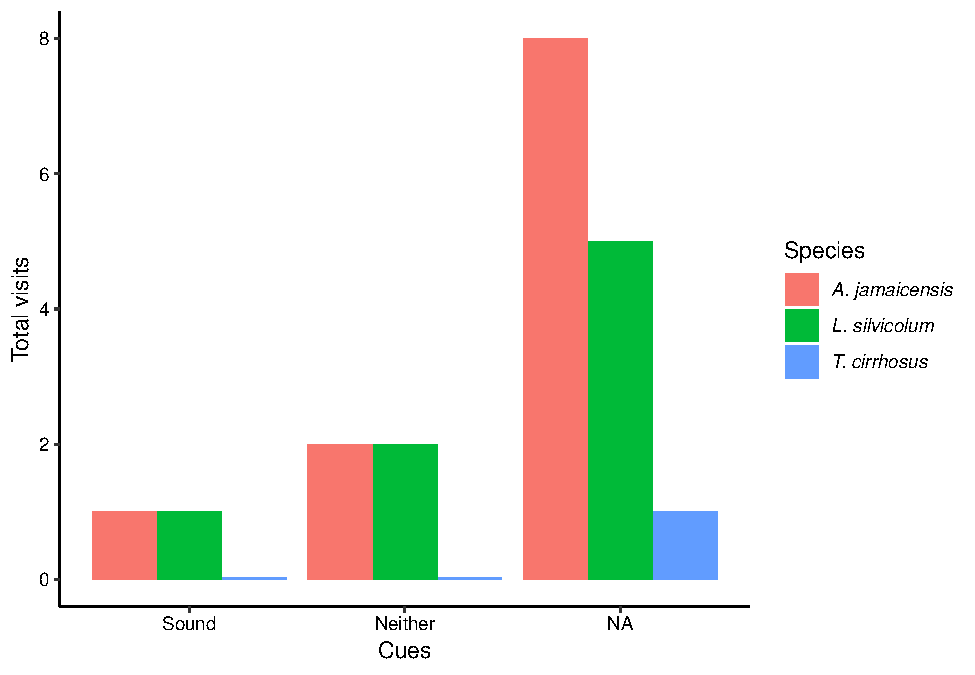
\includegraphics{Sensory_learning_files/figure-latex/unnamed-chunk-27-1.pdf}

\begin{Shaded}
\begin{Highlighting}[]
  \CommentTok{#ggsave("Loc_v_sound_first_visit.png")}
 \CommentTok{# rm(First_visits_p)}
\end{Highlighting}
\end{Shaded}

\section{LOC V SMELL}\label{loc-v-smell}

\subsection{Import data}\label{import-data-1}

\begin{Shaded}
\begin{Highlighting}[]
\KeywordTok{head}\NormalTok{(LocVSmell)}
\end{Highlighting}
\end{Shaded}

\begin{verbatim}
## # A tibble: 6 x 31
##   Bat.ID Scorer Date  Time  Species Treatment Rewarded_loc Rewarded_smell
##   <chr>  <chr>  <chr> <chr> <chr>   <chr>            <dbl> <chr>         
## 1 A-C095 unkno~ 3/30~ 23:56 AJ      LocVSmell           42 sasafrass     
## 2 D-C0B6 unkno~ 3/31~ 22:29 AJ      LocVSmell           42 sasafrass     
## 3 C-C09A unkno~ 4/1/~ <NA>  AJ      LocVSmell           42 sasafrass     
## 4 L-C07F unkno~ 4/30~ 23:13 AJ      LocVSmell           33 cinnamon      
## 5 A-Head Dylan  7/3/~ 19:11 L       LocVSmell           31 cinnamon      
## 6 B-Butt Dylan  6/30~ 19:30 L       LocVSmell           31 cinnamon      
## # ... with 23 more variables: first_hover <chr>, first_land <chr>,
## #   first_visit <chr>, lands_loc <int>, hovers_loc <int>,
## #   visits_loc <int>, lands_smell <int>, hovers_smell <int>,
## #   visits_smell <int>, lands_neither <int>, hovers_neither <int>,
## #   visits_neither <int>, visits_nearest <int>, visits_sassafras <int>,
## #   visits_almond <int>, visits_cinnamon <int>, visits_anise <int>,
## #   total_lands <int>, total_hovers <int>, total_visits <int>,
## #   pct_visits_loc <dbl>, pct_visits_smell <dbl>, pct_visits_neither <dbl>
\end{verbatim}

\begin{Shaded}
\begin{Highlighting}[]
\NormalTok{## make a subset with only lophos and AJs, remove Trachops as factor level}

\NormalTok{LocVSmell_AJ_L=}\StringTok{ }\KeywordTok{subset}\NormalTok{(LocVSmell, LocVSmell$Species !=}\StringTok{ "T"}\NormalTok{)}
\NormalTok{##View(LocVSmell_AJ_L)}
\NormalTok{LocVSmell_AJ_L$Species<-}\StringTok{ }\KeywordTok{factor}\NormalTok{(LocVSmell_AJ_L$Species)}
\KeywordTok{head}\NormalTok{(LocVSmell_AJ_L)}
\end{Highlighting}
\end{Shaded}

\begin{verbatim}
## # A tibble: 6 x 31
##   Bat.ID Scorer Date  Time  Species Treatment Rewarded_loc Rewarded_smell
##   <chr>  <chr>  <chr> <chr> <fct>   <chr>            <dbl> <chr>         
## 1 A-C095 unkno~ 3/30~ 23:56 AJ      LocVSmell           42 sasafrass     
## 2 D-C0B6 unkno~ 3/31~ 22:29 AJ      LocVSmell           42 sasafrass     
## 3 C-C09A unkno~ 4/1/~ <NA>  AJ      LocVSmell           42 sasafrass     
## 4 L-C07F unkno~ 4/30~ 23:13 AJ      LocVSmell           33 cinnamon      
## 5 A-Head Dylan  7/3/~ 19:11 L       LocVSmell           31 cinnamon      
## 6 B-Butt Dylan  6/30~ 19:30 L       LocVSmell           31 cinnamon      
## # ... with 23 more variables: first_hover <chr>, first_land <chr>,
## #   first_visit <chr>, lands_loc <int>, hovers_loc <int>,
## #   visits_loc <int>, lands_smell <int>, hovers_smell <int>,
## #   visits_smell <int>, lands_neither <int>, hovers_neither <int>,
## #   visits_neither <int>, visits_nearest <int>, visits_sassafras <int>,
## #   visits_almond <int>, visits_cinnamon <int>, visits_anise <int>,
## #   total_lands <int>, total_hovers <int>, total_visits <int>,
## #   pct_visits_loc <dbl>, pct_visits_smell <dbl>, pct_visits_neither <dbl>
\end{verbatim}

\begin{Shaded}
\begin{Highlighting}[]
\CommentTok{#levels(LocVSmell_AJ_L$Species)}
\end{Highlighting}
\end{Shaded}

SUMMARIZING AVERAGE proportion of visits to each cue

\begin{Shaded}
\begin{Highlighting}[]
\CommentTok{#  summarize average visits per species using dplyr}
\CommentTok{#  summarize number}
\CommentTok{#  seperate out the species}
\CommentTok{#look at histograms of responses}
\CommentTok{#  run kruskal wallace? Anova with percents? }
\CommentTok{#  Make graphs: percentage choices for each species}
\CommentTok{# }

\NormalTok{Avg_pct_visits<-LocVSmell_AJ_L %>%}\StringTok{ }\KeywordTok{group_by}\NormalTok{(Species) %>%}
\StringTok{      }\KeywordTok{summarise}\NormalTok{(}\DataTypeTok{avg_sound =} \KeywordTok{mean}\NormalTok{(pct_visits_loc, }\DataTypeTok{na.rm=}\OtherTok{TRUE}\NormalTok{), }\DataTypeTok{avg_smell =} \KeywordTok{mean}\NormalTok{(pct_visits_smell, }\DataTypeTok{na.rm=}\OtherTok{TRUE}\NormalTok{),}\DataTypeTok{avg_neither =} \KeywordTok{mean}\NormalTok{(pct_visits_neither, }\DataTypeTok{na.rm=}\OtherTok{TRUE}\NormalTok{) )}
\NormalTok{Avg_pct_visits}
\end{Highlighting}
\end{Shaded}

\begin{verbatim}
## # A tibble: 2 x 4
##   Species avg_sound avg_smell avg_neither
##   <fct>       <dbl>     <dbl>       <dbl>
## 1 AJ          0.560    0.252        0.180
## 2 L           0.738    0.0769       0.189
\end{verbatim}

SUMMARIZING AVERAGE number of of visits overall, per species

\begin{Shaded}
\begin{Highlighting}[]
\NormalTok{### Can also look at the absolute number of times that a given species visits or lands on a platform (total visits)}
\NormalTok{## summary of the mean of the total visits / species mean of the total lands / species, mean of the total hovers/ species}


\NormalTok{Avg_visits_spc<-LocVSmell_AJ_L %>%}\StringTok{ }\KeywordTok{group_by}\NormalTok{(Species) %>%}
\StringTok{      }\KeywordTok{summarise}\NormalTok{(}\DataTypeTok{avg_vis =} \KeywordTok{mean}\NormalTok{(total_visits, }\DataTypeTok{na.rm=}\OtherTok{TRUE}\NormalTok{), }\DataTypeTok{sd_vis =} \KeywordTok{sd}\NormalTok{(total_visits), }\DataTypeTok{avg_lands =} \KeywordTok{mean}\NormalTok{(total_lands, }\DataTypeTok{na.rm=}\OtherTok{TRUE}\NormalTok{), }\DataTypeTok{sd_lands =} \KeywordTok{sd}\NormalTok{(total_lands), }\DataTypeTok{avg_hovers =} \KeywordTok{mean}\NormalTok{(total_hovers, }\DataTypeTok{na.rm=}\OtherTok{TRUE}\NormalTok{), }\DataTypeTok{sd_hovers =} \KeywordTok{sd}\NormalTok{(total_hovers) )}
\NormalTok{Avg_visits_spc}
\end{Highlighting}
\end{Shaded}

\begin{verbatim}
## # A tibble: 2 x 7
##   Species avg_vis sd_vis avg_lands sd_lands avg_hovers sd_hovers
##   <fct>     <dbl>  <dbl>     <dbl>    <dbl>      <dbl>     <dbl>
## 1 AJ         16.7   NA       0.636     NA         15.9      NA  
## 2 L          41.7   26.7    21.2       20.2       20.7      10.6
\end{verbatim}

\begin{Shaded}
\begin{Highlighting}[]
\KeywordTok{class}\NormalTok{(Avg_visits_spc)}
\end{Highlighting}
\end{Shaded}

\begin{verbatim}
## [1] "tbl_df"     "tbl"        "data.frame"
\end{verbatim}

\begin{Shaded}
\begin{Highlighting}[]
\CommentTok{#seems like lophos may go the the platforms more on average. At a glance: }
\KeywordTok{t.test}\NormalTok{(LocVSmell_AJ_L$total_visits[LocVSmell_AJ_L$Species ==}\StringTok{"AJ"}\NormalTok{], LocVSmell_AJ_L$total_visits[LocVSmell_AJ_L$Species ==}\StringTok{"L"}\NormalTok{])}
\end{Highlighting}
\end{Shaded}

\begin{verbatim}
## 
##  Welch Two Sample t-test
## 
## data:  LocVSmell_AJ_L$total_visits[LocVSmell_AJ_L$Species == "AJ"] and LocVSmell_AJ_L$total_visits[LocVSmell_AJ_L$Species == "L"]
## t = -2.6735, df = 12.875, p-value = 0.01927
## alternative hypothesis: true difference in means is not equal to 0
## 95 percent confidence interval:
##  -45.17252  -4.77293
## sample estimates:
## mean of x mean of y 
##  16.72727  41.70000
\end{verbatim}

\begin{Shaded}
\begin{Highlighting}[]
\CommentTok{# At least here, seems that lohpo visit and land more often}
\end{Highlighting}
\end{Shaded}

\subsection{STATS}\label{stats-1}

\subsection{assessing normality}\label{assessing-normality-1}

\begin{Shaded}
\begin{Highlighting}[]
\NormalTok{## basically assessing normality}
\KeywordTok{hist}\NormalTok{(LocVSmell_AJ_L$pct_visits_smell[LocVSmell_AJ_L$Species==}\StringTok{"L"}\NormalTok{], }\DataTypeTok{breaks=}\DecValTok{6}\NormalTok{)}
\end{Highlighting}
\end{Shaded}

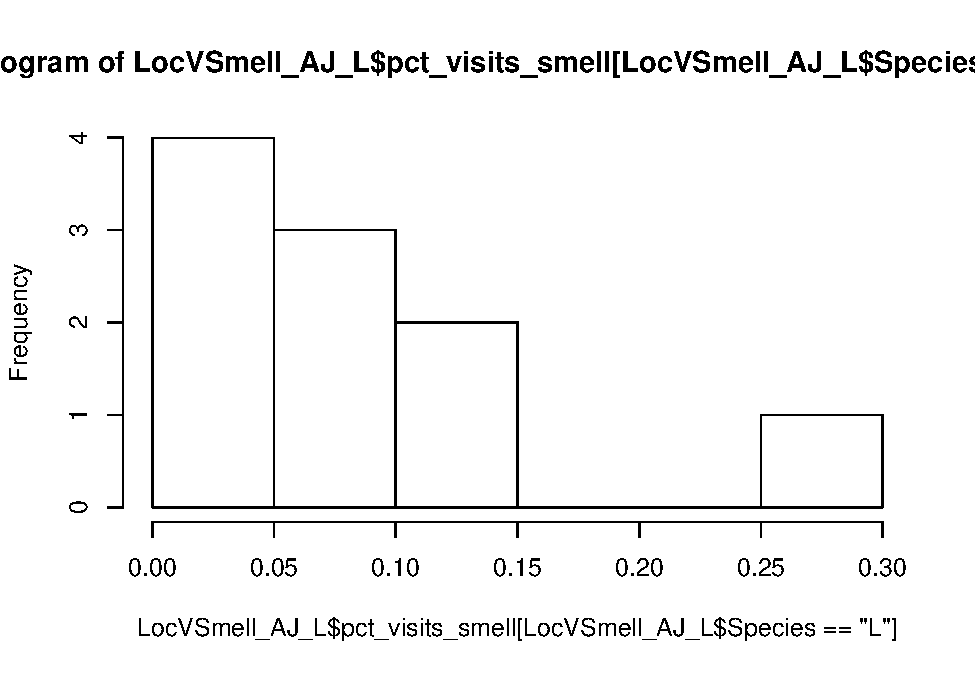
\includegraphics{Sensory_learning_files/figure-latex/unnamed-chunk-31-1.pdf}

\begin{Shaded}
\begin{Highlighting}[]
\CommentTok{#not particularly normal}
\KeywordTok{head}\NormalTok{(LocVSmell_AJ_L)}
\end{Highlighting}
\end{Shaded}

\begin{verbatim}
## # A tibble: 6 x 31
##   Bat.ID Scorer Date  Time  Species Treatment Rewarded_loc Rewarded_smell
##   <chr>  <chr>  <chr> <chr> <fct>   <chr>            <dbl> <chr>         
## 1 A-C095 unkno~ 3/30~ 23:56 AJ      LocVSmell           42 sasafrass     
## 2 D-C0B6 unkno~ 3/31~ 22:29 AJ      LocVSmell           42 sasafrass     
## 3 C-C09A unkno~ 4/1/~ <NA>  AJ      LocVSmell           42 sasafrass     
## 4 L-C07F unkno~ 4/30~ 23:13 AJ      LocVSmell           33 cinnamon      
## 5 A-Head Dylan  7/3/~ 19:11 L       LocVSmell           31 cinnamon      
## 6 B-Butt Dylan  6/30~ 19:30 L       LocVSmell           31 cinnamon      
## # ... with 23 more variables: first_hover <chr>, first_land <chr>,
## #   first_visit <chr>, lands_loc <int>, hovers_loc <int>,
## #   visits_loc <int>, lands_smell <int>, hovers_smell <int>,
## #   visits_smell <int>, lands_neither <int>, hovers_neither <int>,
## #   visits_neither <int>, visits_nearest <int>, visits_sassafras <int>,
## #   visits_almond <int>, visits_cinnamon <int>, visits_anise <int>,
## #   total_lands <int>, total_hovers <int>, total_visits <int>,
## #   pct_visits_loc <dbl>, pct_visits_smell <dbl>, pct_visits_neither <dbl>
\end{verbatim}

Do AJs go to one platform more than another? Do Lophostoma go to any
platforms more than one another? Which? Is there a difference between
AJs and lophostoma? (anova? )

\paragraph{Reshape data for plotting and manipulation with
percents}\label{reshape-data-for-plotting-and-manipulation-with-percents-1}

\begin{Shaded}
\begin{Highlighting}[]
\CommentTok{# pull out just the relevent columns: }
\NormalTok{LocVSmell_AJ_L_pcts<-}\StringTok{ }\NormalTok{LocVSmell_AJ_L[ , }\KeywordTok{c}\NormalTok{(}\StringTok{"Bat.ID"}\NormalTok{, }\StringTok{"Species"}\NormalTok{, }\StringTok{"pct_visits_loc"}\NormalTok{, }\StringTok{"pct_visits_smell"}\NormalTok{, }\StringTok{"pct_visits_neither"} \NormalTok{)]}
\KeywordTok{head}\NormalTok{(LocVSmell_AJ_L_pcts)}
\end{Highlighting}
\end{Shaded}

\begin{verbatim}
## # A tibble: 6 x 5
##   Bat.ID Species pct_visits_loc pct_visits_smell pct_visits_neither
##   <chr>  <fct>            <dbl>            <dbl>              <dbl>
## 1 A-C095 AJ               0.667            0.333             0     
## 2 D-C0B6 AJ               1                0                 0     
## 3 C-C09A AJ               0.692            0.154             0.0769
## 4 L-C07F AJ               0.583            0.208             0.208 
## 5 A-Head L                0.85             0.15              0     
## 6 B-Butt L                0.862            0                 0.138
\end{verbatim}

\begin{Shaded}
\begin{Highlighting}[]
\NormalTok{## Alternatively could just put all the rows I don't want melted into "id" in the following fuction. }
\KeywordTok{colnames}\NormalTok{(LocVSmell_AJ_L_pcts)}
\end{Highlighting}
\end{Shaded}

\begin{verbatim}
## [1] "Bat.ID"             "Species"            "pct_visits_loc"    
## [4] "pct_visits_smell"   "pct_visits_neither"
\end{verbatim}

\begin{Shaded}
\begin{Highlighting}[]
\NormalTok{mLocVSmell <-}\StringTok{ }\KeywordTok{melt}\NormalTok{(LocVSmell_AJ_L_pcts, }\DataTypeTok{id=}\KeywordTok{c}\NormalTok{(}\StringTok{"Bat.ID"}\NormalTok{,}\StringTok{"Species"}\NormalTok{))}
\KeywordTok{head}\NormalTok{(mLocVSmell)}
\end{Highlighting}
\end{Shaded}

\begin{verbatim}
##   Bat.ID Species       variable     value
## 1 A-C095      AJ pct_visits_loc 0.6666667
## 2 D-C0B6      AJ pct_visits_loc 1.0000000
## 3 C-C09A      AJ pct_visits_loc 0.6923077
## 4 L-C07F      AJ pct_visits_loc 0.5833333
## 5 A-Head       L pct_visits_loc 0.8500000
## 6 B-Butt       L pct_visits_loc 0.8620690
\end{verbatim}

\begin{Shaded}
\begin{Highlighting}[]
\CommentTok{#rm(mLocVSmell )}
\end{Highlighting}
\end{Shaded}

\paragraph{Reshape data for plotting and manipulation with
COUNTS}\label{reshape-data-for-plotting-and-manipulation-with-counts-1}

\begin{Shaded}
\begin{Highlighting}[]
\CommentTok{# pull out just the relevent columns: }
\NormalTok{LocVSmell_AJ_L_cnts<-}\StringTok{ }\NormalTok{LocVSmell_AJ_L[ , }\KeywordTok{c}\NormalTok{(}\StringTok{"Bat.ID"}\NormalTok{, }\StringTok{"Species"}\NormalTok{, }\StringTok{"visits_loc"}\NormalTok{, }\StringTok{"visits_smell"}\NormalTok{, }\StringTok{"visits_neither"} \NormalTok{)]}
\KeywordTok{head}\NormalTok{(LocVSmell_AJ_L_cnts)}
\end{Highlighting}
\end{Shaded}

\begin{verbatim}
## # A tibble: 6 x 5
##   Bat.ID Species visits_loc visits_smell visits_neither
##   <chr>  <fct>        <int>        <int>          <int>
## 1 A-C095 AJ               4            2              0
## 2 D-C0B6 AJ               2            0              0
## 3 C-C09A AJ              18            4              2
## 4 L-C07F AJ              14            5              5
## 5 A-Head L               34            6              0
## 6 B-Butt L               25            0              4
\end{verbatim}

\begin{Shaded}
\begin{Highlighting}[]
\NormalTok{## Alternatively could just put all the rows I don't want melted into "id" in the following fuction, which would save the rest of the data}
\KeywordTok{colnames}\NormalTok{(LocVSmell_AJ_L_cnts)}
\end{Highlighting}
\end{Shaded}

\begin{verbatim}
## [1] "Bat.ID"         "Species"        "visits_loc"     "visits_smell"  
## [5] "visits_neither"
\end{verbatim}

\begin{Shaded}
\begin{Highlighting}[]
\NormalTok{mLocVSmell_cnts <-}\StringTok{ }\KeywordTok{melt}\NormalTok{(LocVSmell_AJ_L_cnts, }\DataTypeTok{id=}\KeywordTok{c}\NormalTok{(}\StringTok{"Bat.ID"}\NormalTok{,}\StringTok{"Species"}\NormalTok{))}
\KeywordTok{head}\NormalTok{(mLocVSmell_cnts)}
\end{Highlighting}
\end{Shaded}

\begin{verbatim}
##   Bat.ID Species   variable value
## 1 A-C095      AJ visits_loc     4
## 2 D-C0B6      AJ visits_loc     2
## 3 C-C09A      AJ visits_loc    18
## 4 L-C07F      AJ visits_loc    14
## 5 A-Head       L visits_loc    34
## 6 B-Butt       L visits_loc    25
\end{verbatim}

\begin{Shaded}
\begin{Highlighting}[]
\NormalTok{## convenient also to just add this count value to mLocVSmell}
\NormalTok{visits_counts<-mLocVSmell_cnts$value}
\NormalTok{mLocVSmell <-}\KeywordTok{cbind}\NormalTok{(mLocVSmell, visits_counts)}
\end{Highlighting}
\end{Shaded}

" Did the bats fly to the three platforms the same amount?" AJS \#\#\#\#
Kruskal-wallace: AJ

\begin{Shaded}
\begin{Highlighting}[]
\NormalTok{LvSm_AJ_k.test<-}\StringTok{ }\KeywordTok{kruskal.test}\NormalTok{(value ~}\StringTok{ }\NormalTok{variable, }\DataTypeTok{data =}\NormalTok{mLocVSmell[mLocVSmell$Species ==}\StringTok{"AJ"}\NormalTok{, ] )}
\NormalTok{LvSm_AJ_k.test}
\end{Highlighting}
\end{Shaded}

\begin{verbatim}
## 
##  Kruskal-Wallis rank sum test
## 
## data:  value by variable
## Kruskal-Wallis chi-squared = 12.645, df = 2, p-value = 0.001796
\end{verbatim}

\begin{Shaded}
\begin{Highlighting}[]
\NormalTok{LvSm_AJ_count_k.test<-}\StringTok{ }\KeywordTok{kruskal.test}\NormalTok{(value ~}\StringTok{ }\NormalTok{variable, }\DataTypeTok{data =}\NormalTok{mLocVSmell_cnts[mLocVSmell_cnts$Species ==}\StringTok{"AJ"}\NormalTok{, ] )}
\NormalTok{LvSm_AJ_count_k.test}
\end{Highlighting}
\end{Shaded}

\begin{verbatim}
## 
##  Kruskal-Wallis rank sum test
## 
## data:  value by variable
## Kruskal-Wallis chi-squared = 2.9843, df = 2, p-value = 0.2249
\end{verbatim}

Significant difference, so post-hocs

\paragraph{Kruskal-wallace: Lophos}\label{kruskal-wallace-lophos-1}

\begin{Shaded}
\begin{Highlighting}[]
\NormalTok{LvSm_L_k.test<-}\StringTok{ }\KeywordTok{kruskal.test}\NormalTok{(value ~}\StringTok{ }\NormalTok{variable, }\DataTypeTok{data =}\NormalTok{mLocVSmell[mLocVSmell$Species ==}\StringTok{"L"}\NormalTok{, ] )}

\NormalTok{LvSm_L_k.test}
\end{Highlighting}
\end{Shaded}

\begin{verbatim}
## 
##  Kruskal-Wallis rank sum test
## 
## data:  value by variable
## Kruskal-Wallis chi-squared = 17.112, df = 2, p-value = 0.0001924
\end{verbatim}

\begin{Shaded}
\begin{Highlighting}[]
\NormalTok{LvSm_L_cnts_k.test<-}\StringTok{ }\KeywordTok{kruskal.test}\NormalTok{(value ~}\StringTok{ }\NormalTok{variable, }\DataTypeTok{data =}\NormalTok{mLocVSmell_cnts[mLocVSmell_cnts$Species ==}\StringTok{"L"}\NormalTok{, ] )}

\NormalTok{LvSm_L_cnts_k.test}
\end{Highlighting}
\end{Shaded}

\begin{verbatim}
## 
##  Kruskal-Wallis rank sum test
## 
## data:  value by variable
## Kruskal-Wallis chi-squared = 11.386, df = 2, p-value = 0.00337
\end{verbatim}

Significant difference, so post-hocs

``Which platforms did the bats fly to more, which were different?''

\paragraph{Man- Whitney / Wilcox: AJs}\label{man--whitney-wilcox-ajs-1}

\begin{Shaded}
\begin{Highlighting}[]
\NormalTok{LvSm_AJ_wilhox =}\StringTok{ }\KeywordTok{pairwise.wilcox.test}\NormalTok{(mLocVSmell[mLocVSmell$Species ==}\StringTok{"AJ"}\NormalTok{, ]$value,  mLocVSmell[mLocVSmell$Species ==}\StringTok{"AJ"}\NormalTok{, ]$variable, }\DataTypeTok{p.adjust.method=}\NormalTok{p.adjust.methods)}
\end{Highlighting}
\end{Shaded}

\begin{verbatim}
## Warning in wilcox.test.default(xi, xj, paired = paired, ...): cannot
## compute exact p-value with ties

## Warning in wilcox.test.default(xi, xj, paired = paired, ...): cannot
## compute exact p-value with ties

## Warning in wilcox.test.default(xi, xj, paired = paired, ...): cannot
## compute exact p-value with ties
\end{verbatim}

\begin{Shaded}
\begin{Highlighting}[]
\NormalTok{LvSm_AJ_wilhox}
\end{Highlighting}
\end{Shaded}

\begin{verbatim}
## 
##  Pairwise comparisons using Wilcoxon rank sum test 
## 
## data:  mLocVSmell[mLocVSmell$Species == "AJ", ]$value and mLocVSmell[mLocVSmell$Species == "AJ", ]$variable 
## 
##                    pct_visits_loc pct_visits_smell
## pct_visits_smell   0.0094         -               
## pct_visits_neither 0.0060         0.4515          
## 
## P value adjustment method: holm
\end{verbatim}

\paragraph{Man- Whitney / Wilcox:
Lophos}\label{man--whitney-wilcox-lophos-1}

\begin{Shaded}
\begin{Highlighting}[]
\NormalTok{LvSm_L_wilhox =}\StringTok{ }\KeywordTok{pairwise.wilcox.test}\NormalTok{(mLocVSmell[mLocVSmell$Species ==}\StringTok{"L"}\NormalTok{, ]$value,  mLocVSmell[mLocVSmell$Species ==}\StringTok{"L"}\NormalTok{, ]$variable, }\DataTypeTok{p.adjust.method=}\NormalTok{p.adjust.methods)}
\end{Highlighting}
\end{Shaded}

\begin{verbatim}
## Warning in wilcox.test.default(xi, xj, paired = paired, ...): cannot
## compute exact p-value with ties

## Warning in wilcox.test.default(xi, xj, paired = paired, ...): cannot
## compute exact p-value with ties

## Warning in wilcox.test.default(xi, xj, paired = paired, ...): cannot
## compute exact p-value with ties
\end{verbatim}

\begin{Shaded}
\begin{Highlighting}[]
\NormalTok{LvSm_L_wilhox}
\end{Highlighting}
\end{Shaded}

\begin{verbatim}
## 
##  Pairwise comparisons using Wilcoxon rank sum test 
## 
## data:  mLocVSmell[mLocVSmell$Species == "L", ]$value and mLocVSmell[mLocVSmell$Species == "L", ]$variable 
## 
##                    pct_visits_loc pct_visits_smell
## pct_visits_smell   0.00068        -               
## pct_visits_neither 0.00237        0.60645         
## 
## P value adjustment method: holm
\end{verbatim}

\subsection{Dunn test post hoc: AJ}\label{dunn-test-post-hoc-aj-1}

\begin{Shaded}
\begin{Highlighting}[]
\NormalTok{LvSm_AJ_dunn<-}\KeywordTok{dunnTest}\NormalTok{(mLocVSmell[mLocVSmell$Species ==}\StringTok{"AJ"}\NormalTok{, ]$value,  mLocVSmell[mLocVSmell$Species ==}\StringTok{"AJ"}\NormalTok{, ]$variable, }\DataTypeTok{method=}\StringTok{"holm"}\NormalTok{, }\DataTypeTok{kw=}\OtherTok{TRUE}\NormalTok{)}
\end{Highlighting}
\end{Shaded}

\begin{verbatim}
## Warning: Some rows deleted from 'x' and 'g' because missing data.
\end{verbatim}

\begin{Shaded}
\begin{Highlighting}[]
\NormalTok{LvSm_AJ_dunn}
\end{Highlighting}
\end{Shaded}

\begin{verbatim}
## Dunn (1964) Kruskal-Wallis multiple comparison
\end{verbatim}

\begin{verbatim}
##   p-values adjusted with the Holm method.
\end{verbatim}

\begin{verbatim}
##                              Comparison          Z      P.unadj
## 1   pct_visits_loc - pct_visits_neither  3.3438290 0.0008263064
## 2     pct_visits_loc - pct_visits_smell  2.7196476 0.0065351517
## 3 pct_visits_neither - pct_visits_smell -0.6241814 0.5325084468
##         P.adj
## 1 0.002478919
## 2 0.013070303
## 3 0.532508447
\end{verbatim}

,./\#\#Dunn test post hoc: Lopho

\begin{Shaded}
\begin{Highlighting}[]
\NormalTok{LvSm_L_dunn<-}\KeywordTok{dunnTest}\NormalTok{(mLocVSmell[mLocVSmell$Species ==}\StringTok{"L"}\NormalTok{, ]$value,  mLocVSmell[mLocVSmell$Species ==}\StringTok{"L"}\NormalTok{, ]$variable, }\DataTypeTok{method=}\StringTok{"holm"}\NormalTok{, }\DataTypeTok{kw=}\OtherTok{TRUE}\NormalTok{)}
\NormalTok{LvSm_L_dunn}
\end{Highlighting}
\end{Shaded}

\begin{verbatim}
## Dunn (1964) Kruskal-Wallis multiple comparison
\end{verbatim}

\begin{verbatim}
##   p-values adjusted with the Holm method.
\end{verbatim}

\begin{verbatim}
##                              Comparison         Z      P.unadj
## 1   pct_visits_loc - pct_visits_neither 3.2969971 0.0009772451
## 2     pct_visits_loc - pct_visits_smell 3.8121529 0.0001377616
## 3 pct_visits_neither - pct_visits_smell 0.5151558 0.6064441548
##          P.adj
## 1 0.0019544902
## 2 0.0004132848
## 3 0.6064441548
\end{verbatim}

\paragraph{Nemenyi or Zar or Mann-Whitney tests for post hoc
analyses?}\label{nemenyi-or-zar-or-mann-whitney-tests-for-post-hoc-analyses-1}

\paragraph{Do the different species go to the platforms
equally?}\label{do-the-different-species-go-to-the-platforms-equally-1}

\subsection{Investigating assumptions for ANOVA Trying out
transformations}\label{investigating-assumptions-for-anova-trying-out-transformations-1}

\begin{Shaded}
\begin{Highlighting}[]
\CommentTok{#proportion data}
\KeywordTok{boxplot}\NormalTok{(value ~}\StringTok{  }\NormalTok{variable*}\StringTok{ }\NormalTok{Species, }\DataTypeTok{data =} \NormalTok{mLocVSmell) }\CommentTok{#box width of largest looks more than 2x larger than that of smaller}
\end{Highlighting}
\end{Shaded}

\includegraphics{Sensory_learning_files/figure-latex/unnamed-chunk-41-1.pdf}

\begin{Shaded}
\begin{Highlighting}[]
\KeywordTok{bartlett.test}\NormalTok{( value ~}\StringTok{  }\KeywordTok{interaction}\NormalTok{(variable, Species), }\DataTypeTok{data =} \NormalTok{mLocVSmell) }\CommentTok{#Bartlett test shows variances are different}
\end{Highlighting}
\end{Shaded}

\begin{verbatim}
## 
##  Bartlett test of homogeneity of variances
## 
## data:  value by interaction(variable, Species)
## Bartlett's K-squared = 12.712, df = 5, p-value = 0.02623
\end{verbatim}

\begin{Shaded}
\begin{Highlighting}[]
\CommentTok{# proportions don't have normal variance}

\CommentTok{# Count data also does not have homogenaity of variances}
 \KeywordTok{boxplot}\NormalTok{(value ~}\StringTok{  }\NormalTok{variable*}\StringTok{ }\NormalTok{Species, }\DataTypeTok{data =} \NormalTok{mLocVSmell_cnts)}
\end{Highlighting}
\end{Shaded}

\includegraphics{Sensory_learning_files/figure-latex/unnamed-chunk-41-2.pdf}

\begin{Shaded}
\begin{Highlighting}[]
\KeywordTok{bartlett.test}\NormalTok{( value ~}\StringTok{  }\KeywordTok{interaction}\NormalTok{(variable, Species), }\DataTypeTok{data =} \NormalTok{mLocVSmell_cnts)}
\end{Highlighting}
\end{Shaded}

\begin{verbatim}
## 
##  Bartlett test of homogeneity of variances
## 
## data:  value by interaction(variable, Species)
## Bartlett's K-squared = 30.06, df = 5, p-value = 1.435e-05
\end{verbatim}

\begin{Shaded}
\begin{Highlighting}[]
\CommentTok{# does not have homogenaity of variance}


\NormalTok{mLocVSmell_cnts$value_sqrt<-}\StringTok{ }\NormalTok{(}\KeywordTok{sqrt}\NormalTok{(mLocVSmell_cnts$value)) }\CommentTok{#sqrt transformation}
\NormalTok{mLocVSmell_cnts$value_cub =}\StringTok{ }\KeywordTok{sign}\NormalTok{(mLocVSmell_cnts$value) *}\StringTok{ }\KeywordTok{abs}\NormalTok{(mLocVSmell_cnts$value)^(}\DecValTok{1}\NormalTok{/}\DecValTok{3}\NormalTok{)  }\CommentTok{#cubed transformation}
\NormalTok{mLocVSmell$value_log<-}\StringTok{ }\NormalTok{(}\KeywordTok{log}\NormalTok{(mLocVSmell$value))}\CommentTok{#log transformation- too strong}
\NormalTok{mLocVSmell$value_sqrt<-}\StringTok{ }\NormalTok{(}\KeywordTok{sqrt}\NormalTok{(mLocVSmell$value)) }\CommentTok{#sqrt transformation}
\NormalTok{mLocVSmell$value_cub =}\StringTok{ }\KeywordTok{sign}\NormalTok{(mLocVSmell$value) *}\StringTok{ }\KeywordTok{abs}\NormalTok{(mLocVSmell_cnts$value)^(}\DecValTok{1}\NormalTok{/}\DecValTok{3}\NormalTok{)  }\CommentTok{#cubed transformation}
\NormalTok{mLocVSmell$value_log<-}\StringTok{ }\NormalTok{(}\KeywordTok{log}\NormalTok{(mLocVSmell$value))}\CommentTok{#log transformation- too strong}

\KeywordTok{boxplot}\NormalTok{(value ~}\StringTok{  }\NormalTok{variable*}\StringTok{ }\NormalTok{Species, }\DataTypeTok{data =} \NormalTok{mLocVSmell) }\CommentTok{#original}
\end{Highlighting}
\end{Shaded}

\includegraphics{Sensory_learning_files/figure-latex/unnamed-chunk-41-3.pdf}

\begin{Shaded}
\begin{Highlighting}[]
\KeywordTok{boxplot}\NormalTok{(value_sqrt ~}\StringTok{  }\NormalTok{variable*}\StringTok{ }\NormalTok{Species, }\DataTypeTok{data =} \NormalTok{mLocVSmell) }\CommentTok{#sqrt}
\end{Highlighting}
\end{Shaded}

\includegraphics{Sensory_learning_files/figure-latex/unnamed-chunk-41-4.pdf}

\begin{Shaded}
\begin{Highlighting}[]
\KeywordTok{boxplot}\NormalTok{(value_cub ~}\StringTok{  }\NormalTok{variable*}\StringTok{ }\NormalTok{Species, }\DataTypeTok{data =} \NormalTok{mLocVSmell) }\CommentTok{#cub, pretty good}
\end{Highlighting}
\end{Shaded}

\includegraphics{Sensory_learning_files/figure-latex/unnamed-chunk-41-5.pdf}

\begin{Shaded}
\begin{Highlighting}[]
\KeywordTok{boxplot}\NormalTok{(value_log ~}\StringTok{  }\NormalTok{variable*}\StringTok{ }\NormalTok{Species, }\DataTypeTok{data =} \NormalTok{mLocVSmell) }\CommentTok{# too strong}
\end{Highlighting}
\end{Shaded}

\begin{verbatim}
## Warning in bplt(at[i], wid = width[i], stats = z$stats[, i], out =
## z$out[z$group == : Outlier (-Inf) in boxplot 2 is not drawn
\end{verbatim}

\begin{verbatim}
## Warning in bplt(at[i], wid = width[i], stats = z$stats[, i], out =
## z$out[z$group == : Outlier (-Inf) in boxplot 3 is not drawn
\end{verbatim}

\includegraphics{Sensory_learning_files/figure-latex/unnamed-chunk-41-6.pdf}

\begin{Shaded}
\begin{Highlighting}[]
\CommentTok{#counts}
\KeywordTok{boxplot}\NormalTok{(value ~}\StringTok{  }\NormalTok{variable*}\StringTok{ }\NormalTok{Species, }\DataTypeTok{data =} \NormalTok{mLocVSmell_cnts) }\CommentTok{#original}
\end{Highlighting}
\end{Shaded}

\includegraphics{Sensory_learning_files/figure-latex/unnamed-chunk-41-7.pdf}

\begin{Shaded}
\begin{Highlighting}[]
\KeywordTok{boxplot}\NormalTok{(value_sqrt ~}\StringTok{  }\NormalTok{variable*}\StringTok{ }\NormalTok{Species, }\DataTypeTok{data =} \NormalTok{mLocVSmell_cnts) }\CommentTok{#sqrt, prob best}
\end{Highlighting}
\end{Shaded}

\includegraphics{Sensory_learning_files/figure-latex/unnamed-chunk-41-8.pdf}

\begin{Shaded}
\begin{Highlighting}[]
\KeywordTok{boxplot}\NormalTok{(value_cub ~}\StringTok{  }\NormalTok{variable*}\StringTok{ }\NormalTok{Species, }\DataTypeTok{data =} \NormalTok{mLocVSmell_cnts) }\CommentTok{#cub, }
\end{Highlighting}
\end{Shaded}

\includegraphics{Sensory_learning_files/figure-latex/unnamed-chunk-41-9.pdf}

\begin{Shaded}
\begin{Highlighting}[]
\CommentTok{#boxplot(value_log ~  variable* Species, data = mLocVSmell_cnts) # too strong}

\KeywordTok{bartlett.test}\NormalTok{( value_sqrt ~}\StringTok{  }\KeywordTok{interaction}\NormalTok{(variable, Species), }\DataTypeTok{data =} \NormalTok{mLocVSmell)}
\end{Highlighting}
\end{Shaded}

\begin{verbatim}
## 
##  Bartlett test of homogeneity of variances
## 
## data:  value_sqrt by interaction(variable, Species)
## Bartlett's K-squared = 6.7637, df = 5, p-value = 0.2388
\end{verbatim}

\begin{Shaded}
\begin{Highlighting}[]
\KeywordTok{bartlett.test}\NormalTok{( value_sqrt ~}\StringTok{  }\KeywordTok{interaction}\NormalTok{(variable, Species), }\DataTypeTok{data =} \NormalTok{mLocVSmell_cnts)}
\end{Highlighting}
\end{Shaded}

\begin{verbatim}
## 
##  Bartlett test of homogeneity of variances
## 
## data:  value_sqrt by interaction(variable, Species)
## Bartlett's K-squared = 8.4282, df = 5, p-value = 0.1342
\end{verbatim}

\begin{Shaded}
\begin{Highlighting}[]
\NormalTok{## This actually seems to have fixed the homogenaity of variances problem}

\CommentTok{#normality? Less important, ANOVAs are robust against this violation}
\CommentTok{#proportions: }
\KeywordTok{hist}\NormalTok{(mLocVSmell$value[mLocVSmell$Species==}\StringTok{"L"}\NormalTok{], }\DataTypeTok{breaks=}\DecValTok{6}\NormalTok{)}
\end{Highlighting}
\end{Shaded}

\includegraphics{Sensory_learning_files/figure-latex/unnamed-chunk-41-10.pdf}

\begin{Shaded}
\begin{Highlighting}[]
\KeywordTok{hist}\NormalTok{(mLocVSmell$value_sqrt[mLocVSmell$Species==}\StringTok{"L"}\NormalTok{], }\DataTypeTok{breaks=}\DecValTok{6}\NormalTok{)}
\end{Highlighting}
\end{Shaded}

\includegraphics{Sensory_learning_files/figure-latex/unnamed-chunk-41-11.pdf}

\begin{Shaded}
\begin{Highlighting}[]
\CommentTok{#hist(mLocVSmell$value_cub[mLocVSmell$Species=="L"], breaks=6)}


\CommentTok{#counts:}
\KeywordTok{hist}\NormalTok{(mLocVSmell_cnts$value[mLocVSmell_cnts$Species==}\StringTok{"L"}\NormalTok{], }\DataTypeTok{breaks=}\DecValTok{6}\NormalTok{)}
\end{Highlighting}
\end{Shaded}

\includegraphics{Sensory_learning_files/figure-latex/unnamed-chunk-41-12.pdf}

\begin{Shaded}
\begin{Highlighting}[]
\KeywordTok{hist}\NormalTok{(mLocVSmell_cnts$value_sqrt[mLocVSmell_cnts$Species==}\StringTok{"L"}\NormalTok{], }\DataTypeTok{breaks=}\DecValTok{6}\NormalTok{)}
\end{Highlighting}
\end{Shaded}

\includegraphics{Sensory_learning_files/figure-latex/unnamed-chunk-41-13.pdf}

\begin{Shaded}
\begin{Highlighting}[]
\KeywordTok{hist}\NormalTok{(mLocVSmell_cnts$value_cub[mLocVSmell_cnts$Species==}\StringTok{"L"}\NormalTok{], }\DataTypeTok{breaks=}\DecValTok{6}\NormalTok{)}
\end{Highlighting}
\end{Shaded}

\includegraphics{Sensory_learning_files/figure-latex/unnamed-chunk-41-14.pdf}

\begin{Shaded}
\begin{Highlighting}[]
\CommentTok{#hist(mLocVSmell_cnts$value_log[mLocVSmell_cnts$Species=="L"], breaks=8)}
\KeywordTok{str}\NormalTok{(mLocVSmell_cnts)}
\end{Highlighting}
\end{Shaded}

\begin{verbatim}
## 'data.frame':    66 obs. of  6 variables:
##  $ Bat.ID    : chr  "A-C095" "D-C0B6" "C-C09A" "L-C07F" ...
##  $ Species   : Factor w/ 2 levels "AJ","L": 1 1 1 1 2 2 2 1 1 2 ...
##  $ variable  : Factor w/ 3 levels "visits_loc","visits_smell",..: 1 1 1 1 1 1 1 1 1 1 ...
##  $ value     : int  4 2 18 14 34 25 33 0 0 29 ...
##  $ value_sqrt: num  2 1.41 4.24 3.74 5.83 ...
##  $ value_cub : num  1.59 1.26 2.62 2.41 3.24 ...
\end{verbatim}

\begin{Shaded}
\begin{Highlighting}[]
\KeywordTok{table}\NormalTok{(mLocVSmell_cnts$value)}
\end{Highlighting}
\end{Shaded}

\begin{verbatim}
## 
##  0  2  3  4  5  6  8  9 10 12 13 14 15 16 18 19 20 25 29 33 34 36 42 55 
## 18  4  3  5  4  4  2  1  2  2  1  2  1  2  1  2  1  1  1  2  1  1  1  1
\end{verbatim}

\begin{Shaded}
\begin{Highlighting}[]
\KeywordTok{sum}\NormalTok{(mLocVSmell_cnts$value ==}\StringTok{ }\DecValTok{0}\NormalTok{)}
\end{Highlighting}
\end{Shaded}

\begin{verbatim}
## [1] NA
\end{verbatim}

\begin{Shaded}
\begin{Highlighting}[]
\NormalTok{## the logged values look good but ruin the homogency of variance}
\NormalTok{## }
\NormalTok{##View(mLocVSmell_cnts)}
\end{Highlighting}
\end{Shaded}

\subsection{Anova with transformed count data, type
1,2,3}\label{anova-with-transformed-count-data-type-123}

\begin{Shaded}
\begin{Highlighting}[]
\KeywordTok{library}\NormalTok{(car)}
\NormalTok{anova_LvSm <-}\StringTok{ }\KeywordTok{aov}\NormalTok{(value_sqrt ~}\StringTok{ }\NormalTok{Species*variable, }\DataTypeTok{data=}\NormalTok{mLocVSmell_cnts)}
\NormalTok{anova_LvSm}
\end{Highlighting}
\end{Shaded}

\begin{verbatim}
## Call:
##    aov(formula = value_sqrt ~ Species * variable, data = mLocVSmell_cnts)
## 
## Terms:
##                   Species  variable Species:variable Residuals
## Sum of Squares   16.20933  54.09942         21.20349 154.71499
## Deg. of Freedom         1         2                2        57
## 
## Residual standard error: 1.647513
## Estimated effects may be unbalanced
## 3 observations deleted due to missingness
\end{verbatim}

\begin{Shaded}
\begin{Highlighting}[]
\KeywordTok{Anova}\NormalTok{(anova_LvSm, }\DataTypeTok{type =} \DecValTok{2}\NormalTok{)}
\end{Highlighting}
\end{Shaded}

\begin{verbatim}
## Anova Table (Type II tests)
## 
## Response: value_sqrt
##                   Sum Sq Df F value    Pr(>F)    
## Species           16.209  1  5.9718 0.0176548 *  
## variable          54.099  2  9.9656 0.0001943 ***
## Species:variable  21.203  2  3.9059 0.0257215 *  
## Residuals        154.715 57                      
## ---
## Signif. codes:  0 '***' 0.001 '**' 0.01 '*' 0.05 '.' 0.1 ' ' 1
\end{verbatim}

\begin{Shaded}
\begin{Highlighting}[]
\KeywordTok{Anova}\NormalTok{(anova_LvSm, }\DataTypeTok{type =} \DecValTok{3}\NormalTok{)}
\end{Highlighting}
\end{Shaded}

\begin{verbatim}
## Anova Table (Type III tests)
## 
## Response: value_sqrt
##                   Sum Sq Df F value    Pr(>F)    
## (Intercept)       67.172  1 24.7475 6.352e-06 ***
## Species           33.782  1 12.4458 0.0008356 ***
## variable           6.257  2  1.1525 0.3230801    
## Species:variable  21.203  2  3.9059 0.0257215 *  
## Residuals        154.715 57                      
## ---
## Signif. codes:  0 '***' 0.001 '**' 0.01 '*' 0.05 '.' 0.1 ' ' 1
\end{verbatim}

\subsection{confidence intervals and
bootstrapping}\label{confidence-intervals-and-bootstrapping-1}

\begin{Shaded}
\begin{Highlighting}[]
\NormalTok{## Could get the mean proportion of visits to cues from each of the species. bootstrap the mean proportion, then compare the 95% confidence intervals for each mean }
\NormalTok{############CODE FROM BASTI#################################################}

\CommentTok{#X will be the vector of proportions or rates or counts for one treatment in a species. It will calculate 5000 means based on re-sampling your data and then calculate the confidence intervals from that mean-distribution. }

\CommentTok{#The function spits out a vector of three values, the lower CI, mean, and upper CI.}

\CommentTok{#This is the function used for it:}
\CommentTok{#https://www.rdocumentation.org/packages/boot/versions/1.3-20/topics/boot.ci}
\NormalTok{###########################################################################}

\CommentTok{#mean function}
\NormalTok{mean.w <-}\StringTok{ }\NormalTok{function(x,w) }\KeywordTok{sum}\NormalTok{(x*w) }\CommentTok{# calculates a mean}

\CommentTok{#bootstrapped confidence intervals function}
\NormalTok{boot_ci <-}\StringTok{ }\NormalTok{function(x)\{}
    \NormalTok{mean <-}\StringTok{ }\KeywordTok{mean}\NormalTok{(x)}
    \NormalTok{low <-}\StringTok{ }\KeywordTok{boot.ci}\NormalTok{(}\KeywordTok{boot}\NormalTok{(}\DataTypeTok{data=}\NormalTok{x, }\DataTypeTok{statistic=}\NormalTok{mean.w, }\DataTypeTok{R=}\DecValTok{5000}\NormalTok{, }\DataTypeTok{stype=}\StringTok{"w"}\NormalTok{), }\DataTypeTok{type=}\StringTok{"basic"}\NormalTok{)$basic[}\DecValTok{1}\NormalTok{,}\DecValTok{4}\NormalTok{]}
    \NormalTok{high <-}\StringTok{ }\KeywordTok{boot.ci}\NormalTok{(}\KeywordTok{boot}\NormalTok{(}\DataTypeTok{data=}\NormalTok{x, }\DataTypeTok{statistic=}\NormalTok{mean.w, }\DataTypeTok{R=}\DecValTok{5000}\NormalTok{, }\DataTypeTok{stype=}\StringTok{"w"}\NormalTok{), }\DataTypeTok{type=}\StringTok{"basic"}\NormalTok{)$basic[}\DecValTok{1}\NormalTok{,}\DecValTok{5}\NormalTok{]}
    \KeywordTok{c}\NormalTok{(low,mean,high)\} }\CommentTok{# bootstraps the confidence intervals}



\NormalTok{## get rid of NAs in data using complete.cases}
\NormalTok{mLocVSmell_na<-mLocVSmell[}\KeywordTok{complete.cases}\NormalTok{(mLocVSmell[ ,}\DecValTok{4}\NormalTok{:}\DecValTok{8}\NormalTok{]), ] }\CommentTok{#removes NA rows in value columns 4:6, this might not make sense if I change the number of columns}
\KeywordTok{head}\NormalTok{(mLocVSmell)}
\end{Highlighting}
\end{Shaded}

\begin{verbatim}
##   Bat.ID Species       variable     value visits_counts  value_log
## 1 A-C095      AJ pct_visits_loc 0.6666667             4 -0.4054651
## 2 D-C0B6      AJ pct_visits_loc 1.0000000             2  0.0000000
## 3 C-C09A      AJ pct_visits_loc 0.6923077            18 -0.3677248
## 4 L-C07F      AJ pct_visits_loc 0.5833333            14 -0.5389965
## 5 A-Head       L pct_visits_loc 0.8500000            34 -0.1625189
## 6 B-Butt       L pct_visits_loc 0.8620690            25 -0.1484200
##   value_sqrt value_cub
## 1  0.8164966  1.587401
## 2  1.0000000  1.259921
## 3  0.8320503  2.620741
## 4  0.7637626  2.410142
## 5  0.9219544  3.239612
## 6  0.9284767  2.924018
\end{verbatim}

\begin{Shaded}
\begin{Highlighting}[]
\CommentTok{#New database without NAs in the selected columns}
\NormalTok{LocVSmell_AJ_L_na <-}\StringTok{ }\NormalTok{LocVSmell_AJ_L[}\KeywordTok{complete.cases}\NormalTok{(LocVSmell_AJ_L[ ,}\KeywordTok{c}\NormalTok{(}\StringTok{"visits_loc"}\NormalTok{, }\StringTok{"visits_smell"}\NormalTok{,  }\StringTok{"visits_neither"}\NormalTok{, }\StringTok{"pct_visits_loc"}\NormalTok{, }\StringTok{"pct_visits_smell"}\NormalTok{, }\StringTok{"pct_visits_neither"}\NormalTok{)]), ]}

\CommentTok{#The CI's for sound v Smell, percentages}
\KeywordTok{set.seed}\NormalTok{(}\DecValTok{1}\NormalTok{)}
\NormalTok{LvSm_pct_CI <-}\StringTok{ }\KeywordTok{do.call}\NormalTok{(data.frame,}\KeywordTok{aggregate}\NormalTok{(value ~}\StringTok{ }\NormalTok{Species +}\StringTok{ }\NormalTok{variable , boot_ci, }\DataTypeTok{data =} \NormalTok{mLocVSmell_na)) }\CommentTok{#This applies the bootstrap accross species and treatment variables, and do.call puts the data.frame in the right format}
\KeywordTok{colnames}\NormalTok{(LvSm_pct_CI) <-}\StringTok{ }\KeywordTok{c}\NormalTok{(}\StringTok{"Species"}\NormalTok{, }\StringTok{"variable"}\NormalTok{, }\StringTok{"low"}\NormalTok{, }\StringTok{"mean"}\NormalTok{, }\StringTok{"high"}\NormalTok{)}

\CommentTok{# The CIs for sound V Smell, counts}
\NormalTok{LvSm_count_CI <-}\StringTok{ }\KeywordTok{do.call}\NormalTok{(data.frame, }\KeywordTok{aggregate}\NormalTok{(visits_counts ~}\StringTok{ }\NormalTok{Species +}\StringTok{ }\NormalTok{variable , boot_ci, }\DataTypeTok{data =} \NormalTok{mLocVSmell_na))}
\KeywordTok{head}\NormalTok{(LvSm_count_CI)}
\end{Highlighting}
\end{Shaded}

\begin{verbatim}
##   Species           variable visits_counts.V1 visits_counts.V2
## 1      AJ     pct_visits_loc         6.111111        10.111111
## 2       L     pct_visits_loc        17.900000        26.600000
## 3      AJ   pct_visits_smell         2.444444         6.000000
## 4       L   pct_visits_smell         0.400000         4.200000
## 5      AJ pct_visits_neither         2.111111         4.111111
## 6       L pct_visits_neither         1.300000        11.100000
##   visits_counts.V3
## 1        14.000000
## 2        33.900000
## 3         9.111111
## 4         6.900000
## 5         6.000000
## 6        19.697492
\end{verbatim}

\begin{Shaded}
\begin{Highlighting}[]
\KeywordTok{colnames}\NormalTok{(LvSm_count_CI) <-}\StringTok{ }\KeywordTok{c}\NormalTok{(}\StringTok{"Species"}\NormalTok{, }\StringTok{"variable"}\NormalTok{, }\StringTok{"low"}\NormalTok{, }\StringTok{"mean"}\NormalTok{, }\StringTok{"high"}\NormalTok{)}
\end{Highlighting}
\end{Shaded}

\subsection{Plotting}\label{plotting-1}

\subsection{plotting confidence intervals for pct and \% visits to
platforms}\label{plotting-confidence-intervals-for-pct-and-visits-to-platforms}

\begin{Shaded}
\begin{Highlighting}[]
\CommentTok{#LvSm_pct_CI$Species <- factor(LvSm_pct_CI$Species, levels=c("AJ", "L"), labels = c("A. jamaicensis", "L. silvicolum")) #need to do this for plot legends to say full name}

\CommentTok{#LvSm_count_CI$Species <- factor(LvSm_count_CI$Species, levels=c("AJ", "L"), labels = c("A. jamaicensis", "L. silvicolum"))}


\NormalTok{pd =}\StringTok{ }\KeywordTok{position_dodge}\NormalTok{(}\FloatTok{0.5}\NormalTok{) }\CommentTok{# move bars .05 to the left and right}

\CommentTok{#proportion plot}
\NormalTok{LvSm_pct_CI_p <-}\StringTok{ }\KeywordTok{ggplot}\NormalTok{(}\DataTypeTok{data =} \NormalTok{LvSm_pct_CI, }\KeywordTok{aes}\NormalTok{(}\DataTypeTok{x=}\NormalTok{variable, }\DataTypeTok{y =} \NormalTok{mean, }\DataTypeTok{colour =} \NormalTok{Species))}
\NormalTok{LvSm_pct_CI_p <-}\StringTok{ }\NormalTok{LvSm_pct_CI_p +}\StringTok{ }\KeywordTok{geom_errorbar}\NormalTok{(}\KeywordTok{aes}\NormalTok{(}\DataTypeTok{ymin =} \NormalTok{low, }\DataTypeTok{ymax =} \NormalTok{high), }\DataTypeTok{width =}\NormalTok{.}\DecValTok{1}\NormalTok{, }\DataTypeTok{position =} \NormalTok{pd)}
\NormalTok{LvSm_pct_CI_p <-}\StringTok{ }\NormalTok{LvSm_pct_CI_p +}\StringTok{ }\KeywordTok{geom_point}\NormalTok{( }\DataTypeTok{position =} \NormalTok{pd, }\DataTypeTok{shape=}\DecValTok{18}\NormalTok{, }\DataTypeTok{size =} \DecValTok{3}\NormalTok{)}
\NormalTok{LvSm_pct_CI_p <-}\StringTok{ }\NormalTok{LvSm_pct_CI_p +}\StringTok{ }\KeywordTok{scale_fill_discrete}\NormalTok{(}\DataTypeTok{name=}\StringTok{"My new legend"}\NormalTok{, }\DataTypeTok{labels =} \KeywordTok{c}\NormalTok{(}\StringTok{"AJ"} \NormalTok{=}\StringTok{ "A. jamaicensis"}\NormalTok{, }\StringTok{"L"} \NormalTok{=}\StringTok{ "L. silvicolum"}\NormalTok{)) }
\NormalTok{LvSm_pct_CI_p <-}\StringTok{ }\NormalTok{LvSm_pct_CI_p +}\StringTok{ }\KeywordTok{theme}\NormalTok{(}\DataTypeTok{panel.grid.major =} \KeywordTok{element_blank}\NormalTok{(), }\DataTypeTok{panel.grid.minor =} \KeywordTok{element_blank}\NormalTok{(),}
\DataTypeTok{panel.background =} \KeywordTok{element_blank}\NormalTok{(), }\DataTypeTok{axis.line =} \KeywordTok{element_line}\NormalTok{(}\DataTypeTok{colour =} \StringTok{"black"}\NormalTok{), }\DataTypeTok{axis.text =} \KeywordTok{element_text}\NormalTok{(}\DataTypeTok{colour =} \StringTok{"black"}\NormalTok{), }\DataTypeTok{legend.text =} \KeywordTok{element_text}\NormalTok{(}\DataTypeTok{face =} \StringTok{"italic"}\NormalTok{))  }\CommentTok{#gets rid of background, makes legend italic}

\NormalTok{LvSm_pct_CI_p <-}\StringTok{ }\NormalTok{LvSm_pct_CI_p +}\StringTok{ }\KeywordTok{scale_x_discrete}\NormalTok{(}\DataTypeTok{labels=}\KeywordTok{c}\NormalTok{(}\StringTok{"pct_visits_sound"} \NormalTok{=}\StringTok{ "Location"}\NormalTok{, }\StringTok{"pct_visits_smell"} \NormalTok{=}\StringTok{ "Smell"}\NormalTok{,}
                              \StringTok{"pct_visits_neither"} \NormalTok{=}\StringTok{ "Neither"} \NormalTok{))  }\CommentTok{# Relabelling X axis}
\NormalTok{LvSm_pct_CI_p <-}\StringTok{ }\NormalTok{LvSm_pct_CI_p +}\StringTok{ }\KeywordTok{xlab}\NormalTok{(}\StringTok{"Cues"}\NormalTok{)}
\NormalTok{LvSm_pct_CI_p <-}\StringTok{ }\NormalTok{LvSm_pct_CI_p +}\StringTok{ }\KeywordTok{ylab}\NormalTok{(}\StringTok{"Mean proportion of visits"}\NormalTok{)}
\NormalTok{LvSm_pct_CI_p <-}\StringTok{ }\NormalTok{LvSm_pct_CI_p +}\StringTok{ }\KeywordTok{scale_color_manual}\NormalTok{(}\DataTypeTok{values =} \KeywordTok{c}\NormalTok{(Lo, Art), }\DataTypeTok{labels =} \KeywordTok{c}\NormalTok{(}\StringTok{"AJ"} \NormalTok{=}\StringTok{ "A. jamaicensis"}\NormalTok{, }\StringTok{"L"} \NormalTok{=}\StringTok{ "L. silvicolum"}\NormalTok{))}
\NormalTok{LvSm_pct_CI_p                    }
\end{Highlighting}
\end{Shaded}

\includegraphics{Sensory_learning_files/figure-latex/unnamed-chunk-44-1.pdf}

\begin{Shaded}
\begin{Highlighting}[]
\CommentTok{#ggsave("LvSm_pct_CI_p.png")}

\CommentTok{#count plot}
\NormalTok{LvSm_count_CI_p <-}\StringTok{ }\KeywordTok{ggplot}\NormalTok{(}\DataTypeTok{data =} \NormalTok{LvSm_count_CI, }\KeywordTok{aes}\NormalTok{(}\DataTypeTok{x=}\NormalTok{variable, }\DataTypeTok{y =} \NormalTok{mean, }\DataTypeTok{colour =} \NormalTok{Species))}
\NormalTok{LvSm_count_CI_p <-}\StringTok{ }\NormalTok{LvSm_count_CI_p +}\StringTok{ }\KeywordTok{geom_errorbar}\NormalTok{(}\KeywordTok{aes}\NormalTok{(}\DataTypeTok{ymin =} \NormalTok{low, }\DataTypeTok{ymax =} \NormalTok{high), }\DataTypeTok{width =}\NormalTok{.}\DecValTok{1}\NormalTok{, }\DataTypeTok{position =} \NormalTok{pd)}
\NormalTok{LvSm_count_CI_p <-}\StringTok{ }\NormalTok{LvSm_count_CI_p +}\StringTok{ }\KeywordTok{geom_point}\NormalTok{( }\DataTypeTok{position =} \NormalTok{pd, }\DataTypeTok{shape=}\DecValTok{18}\NormalTok{, }\DataTypeTok{size =} \DecValTok{3}\NormalTok{)}
\NormalTok{LvSm_count_CI_p <-}\StringTok{ }\NormalTok{LvSm_count_CI_p +}\StringTok{ }\KeywordTok{scale_fill_discrete}\NormalTok{(}\DataTypeTok{name=}\StringTok{"My new legend"}\NormalTok{, }\DataTypeTok{labels =} \KeywordTok{c}\NormalTok{(}\StringTok{"AJ"} \NormalTok{=}\StringTok{ "A. jamaicensis"}\NormalTok{, }\StringTok{"L"} \NormalTok{=}\StringTok{ "L. silvicolum"}\NormalTok{)) }
\NormalTok{LvSm_count_CI_p <-}\StringTok{ }\NormalTok{LvSm_count_CI_p +}\StringTok{ }\KeywordTok{theme}\NormalTok{(}\DataTypeTok{panel.grid.major =} \KeywordTok{element_blank}\NormalTok{(), }\DataTypeTok{panel.grid.minor =} \KeywordTok{element_blank}\NormalTok{(),}
\DataTypeTok{panel.background =} \KeywordTok{element_blank}\NormalTok{(), }\DataTypeTok{axis.line =} \KeywordTok{element_line}\NormalTok{(}\DataTypeTok{colour =} \StringTok{"black"}\NormalTok{), }\DataTypeTok{axis.text =} \KeywordTok{element_text}\NormalTok{(}\DataTypeTok{colour =} \StringTok{"black"}\NormalTok{), }\DataTypeTok{legend.text =} \KeywordTok{element_text}\NormalTok{(}\DataTypeTok{face =} \StringTok{"italic"}\NormalTok{))  }\CommentTok{#gets rid of background, makes legend italic}

\NormalTok{LvSm_count_CI_p <-}\StringTok{ }\NormalTok{LvSm_count_CI_p +}\StringTok{ }\KeywordTok{scale_x_discrete}\NormalTok{(}\DataTypeTok{labels=}\KeywordTok{c}\NormalTok{(}\StringTok{"pct_visits_loc"} \NormalTok{=}\StringTok{ "Location"}\NormalTok{, }\StringTok{"pct_visits_smell"} \NormalTok{=}\StringTok{ "Smell"}\NormalTok{,}
                              \StringTok{"pct_visits_neither"} \NormalTok{=}\StringTok{ "Neither"} \NormalTok{))  }\CommentTok{# Relabelling X axis}
\NormalTok{LvSm_count_CI_p <-}\StringTok{ }\NormalTok{LvSm_count_CI_p +}\StringTok{ }\KeywordTok{xlab}\NormalTok{(}\StringTok{"Cues"}\NormalTok{)}
\NormalTok{LvSm_count_CI_p <-}\StringTok{ }\NormalTok{LvSm_count_CI_p +}\StringTok{ }\KeywordTok{ylab}\NormalTok{(}\StringTok{"Mean number of visits"}\NormalTok{)}
\NormalTok{LvSm_count_CI_p <-}\StringTok{ }\NormalTok{LvSm_count_CI_p +}\StringTok{ }\KeywordTok{scale_color_manual}\NormalTok{(}\DataTypeTok{values =} \KeywordTok{c}\NormalTok{(Lo, Art), }\DataTypeTok{labels =} \KeywordTok{c}\NormalTok{(}\StringTok{"AJ"} \NormalTok{=}\StringTok{ "A. jamaicensis"}\NormalTok{, }\StringTok{"L"} \NormalTok{=}\StringTok{ "L. silvicolum"}\NormalTok{))}
\NormalTok{LvSm_count_CI_p }
\end{Highlighting}
\end{Shaded}

\includegraphics{Sensory_learning_files/figure-latex/unnamed-chunk-44-2.pdf}

\begin{Shaded}
\begin{Highlighting}[]
\CommentTok{#ggsave("LvSm_count_CI_p.png" )}
\end{Highlighting}
\end{Shaded}

\section{check out nearest. Is there a weird
value?}\label{check-out-nearest.-is-there-a-weird-value}

\paragraph{Plotting \% of visits to the different platforms,
LvSm}\label{plotting-of-visits-to-the-different-platforms-lvsm}

\begin{Shaded}
\begin{Highlighting}[]
\NormalTok{LocVSmell_bar <-}\StringTok{ }\KeywordTok{ggplot}\NormalTok{(}\DataTypeTok{data =}\NormalTok{mLocVSmell, }\KeywordTok{aes}\NormalTok{(}\DataTypeTok{x =} \NormalTok{variable, }\DataTypeTok{y =} \NormalTok{value))}
\NormalTok{LocVSmell_bar <-}\StringTok{ }\NormalTok{LocVSmell_bar +}\StringTok{ }\KeywordTok{geom_boxplot}\NormalTok{(}\KeywordTok{aes}\NormalTok{(}\DataTypeTok{fill=}\NormalTok{Species))}
\NormalTok{LocVSmell_bar <-}\StringTok{ }\NormalTok{LocVSmell_bar +}\StringTok{ }\KeywordTok{geom_point}\NormalTok{(}\DataTypeTok{position=}\KeywordTok{position_dodge}\NormalTok{(}\DataTypeTok{width=}\FloatTok{0.75}\NormalTok{), }\KeywordTok{aes}\NormalTok{(}\DataTypeTok{group=}\NormalTok{Species), }\DataTypeTok{alpha =} \DecValTok{1}\NormalTok{/}\DecValTok{4}\NormalTok{) }\CommentTok{#makes points semi-transparent}
\NormalTok{LocVSmell_bar <-}\StringTok{ }\NormalTok{LocVSmell_bar +}\StringTok{ }\KeywordTok{theme}\NormalTok{(}\DataTypeTok{panel.grid.major =} \KeywordTok{element_blank}\NormalTok{(), }\DataTypeTok{panel.grid.minor =} \KeywordTok{element_blank}\NormalTok{(),}
\DataTypeTok{panel.background =} \KeywordTok{element_blank}\NormalTok{(), }\DataTypeTok{axis.line =} \KeywordTok{element_line}\NormalTok{(}\DataTypeTok{colour =} \StringTok{"black"}\NormalTok{), }\DataTypeTok{axis.text =} \KeywordTok{element_text}\NormalTok{(}\DataTypeTok{colour =} \StringTok{"black"}\NormalTok{), }\DataTypeTok{legend.text =} \KeywordTok{element_text}\NormalTok{(}\DataTypeTok{face =} \StringTok{"italic"}\NormalTok{))  }\CommentTok{#gets rid of background, makes legend italic}
\NormalTok{LocVSmell_bar <-}\StringTok{ }\NormalTok{LocVSmell_bar +}\StringTok{ }\KeywordTok{xlab}\NormalTok{(}\StringTok{"Cues"}\NormalTok{)}
\NormalTok{LocVSmell_bar <-}\StringTok{ }\NormalTok{LocVSmell_bar +}\StringTok{ }\KeywordTok{ylab}\NormalTok{(}\StringTok{"Proportion of total visits"}\NormalTok{)}
\NormalTok{LocVSmell_bar <-}\StringTok{ }\NormalTok{LocVSmell_bar +}\StringTok{ }\KeywordTok{scale_x_discrete}\NormalTok{(}\DataTypeTok{labels=}\KeywordTok{c}\NormalTok{(}\StringTok{"pct_visits_sound"} \NormalTok{=}\StringTok{ "Location"}\NormalTok{, }\StringTok{"pct_visits_smell"} \NormalTok{=}\StringTok{ "Smell"}\NormalTok{,}
                              \StringTok{"pct_visits_neither"} \NormalTok{=}\StringTok{ "Neither"} \NormalTok{))  }\CommentTok{# Relabelling X axis}
\NormalTok{LocVSmell_bar <-}\StringTok{ }\NormalTok{LocVSmell_bar +}\StringTok{  }\KeywordTok{scale_fill_manual}\NormalTok{(}\DataTypeTok{values =} \KeywordTok{c}\NormalTok{(Lo, Art), }\DataTypeTok{labels =} \KeywordTok{c}\NormalTok{(}\StringTok{"AJ"} \NormalTok{=}\StringTok{ "A. jamaicensis"}\NormalTok{, }\StringTok{"L"} \NormalTok{=}\StringTok{ "L. silvicolum"}\NormalTok{))}
\NormalTok{LocVSmell_bar}
\end{Highlighting}
\end{Shaded}

\begin{verbatim}
## Warning: Removed 9 rows containing non-finite values (stat_boxplot).
\end{verbatim}

\begin{verbatim}
## Warning: Removed 9 rows containing missing values (geom_point).
\end{verbatim}

\includegraphics{Sensory_learning_files/figure-latex/unnamed-chunk-45-1.pdf}

\begin{Shaded}
\begin{Highlighting}[]
\NormalTok{##ggsave("LocVSmell.png")}
\end{Highlighting}
\end{Shaded}

\paragraph{Plotting absolute number of visits to the different
platforms}\label{plotting-absolute-number-of-visits-to-the-different-platforms-1}

\begin{Shaded}
\begin{Highlighting}[]
\NormalTok{LocVSmell_bar_cnts <-}\StringTok{ }\KeywordTok{ggplot}\NormalTok{(}\DataTypeTok{data =}\NormalTok{mLocVSmell_cnts, }\KeywordTok{aes}\NormalTok{(}\DataTypeTok{x =} \NormalTok{variable, }\DataTypeTok{y =} \NormalTok{value))}
\NormalTok{LocVSmell_bar_cnts <-}\StringTok{ }\NormalTok{LocVSmell_bar_cnts +}\StringTok{ }\KeywordTok{geom_boxplot}\NormalTok{(}\KeywordTok{aes}\NormalTok{(}\DataTypeTok{fill=}\NormalTok{Species))}
\NormalTok{LocVSmell_bar_cnts <-}\StringTok{ }\NormalTok{LocVSmell_bar_cnts +}\StringTok{ }\KeywordTok{geom_point}\NormalTok{(}\DataTypeTok{position=}\KeywordTok{position_dodge}\NormalTok{(}\DataTypeTok{width=}\FloatTok{0.75}\NormalTok{), }\KeywordTok{aes}\NormalTok{(}\DataTypeTok{group=}\NormalTok{Species), }\DataTypeTok{alpha =} \DecValTok{1}\NormalTok{/}\DecValTok{4}\NormalTok{) }\CommentTok{#makes points semi-transparent}
\NormalTok{LocVSmell_bar_cnts <-}\StringTok{ }\NormalTok{LocVSmell_bar_cnts +}\StringTok{ }\KeywordTok{theme}\NormalTok{(}\DataTypeTok{panel.grid.major =} \KeywordTok{element_blank}\NormalTok{(), }\DataTypeTok{panel.grid.minor =} \KeywordTok{element_blank}\NormalTok{(),}
\DataTypeTok{panel.background =} \KeywordTok{element_blank}\NormalTok{(), }\DataTypeTok{axis.line =} \KeywordTok{element_line}\NormalTok{(}\DataTypeTok{colour =} \StringTok{"black"}\NormalTok{), }\DataTypeTok{axis.text =} \KeywordTok{element_text}\NormalTok{(}\DataTypeTok{colour =} \StringTok{"black"}\NormalTok{), }\DataTypeTok{legend.text =} \KeywordTok{element_text}\NormalTok{(}\DataTypeTok{face =} \StringTok{"italic"}\NormalTok{))  }\CommentTok{#gets rid of background, makes legend italic}
\NormalTok{LocVSmell_bar_cnts <-}\StringTok{ }\NormalTok{LocVSmell_bar_cnts +}\StringTok{ }\KeywordTok{xlab}\NormalTok{(}\StringTok{"Cues"}\NormalTok{)}
\NormalTok{LocVSmell_bar_cnts <-}\StringTok{ }\NormalTok{LocVSmell_bar_cnts +}\StringTok{ }\KeywordTok{ylab}\NormalTok{(}\StringTok{"Number of visits"}\NormalTok{)}
\NormalTok{LocVSmell_bar_cnts <-}\StringTok{ }\NormalTok{LocVSmell_bar_cnts +}\StringTok{ }\KeywordTok{scale_x_discrete}\NormalTok{(}\DataTypeTok{labels=}\KeywordTok{c}\NormalTok{(}\StringTok{"visits_loc"} \NormalTok{=}\StringTok{ "Location"}\NormalTok{, }\StringTok{"visits_smell"} \NormalTok{=}\StringTok{ "Smell"}\NormalTok{,}
                              \StringTok{"visits_neither"} \NormalTok{=}\StringTok{ "Neither"} \NormalTok{))  }\CommentTok{# Relabelling X axis}
\NormalTok{LocVSmell_bar_cnts <-}\StringTok{ }\NormalTok{LocVSmell_bar_cnts +}\StringTok{  }\KeywordTok{scale_fill_manual}\NormalTok{(}\DataTypeTok{values =} \KeywordTok{c}\NormalTok{(Lo, Art), }\DataTypeTok{labels =} \KeywordTok{c}\NormalTok{(}\StringTok{"AJ"} \NormalTok{=}\StringTok{ "A. jamaicensis"}\NormalTok{, }\StringTok{"L"} \NormalTok{=}\StringTok{ "L. silvicolum"}\NormalTok{))}
\NormalTok{LocVSmell_bar_cnts}
\end{Highlighting}
\end{Shaded}

\begin{verbatim}
## Warning: Removed 3 rows containing non-finite values (stat_boxplot).
\end{verbatim}

\begin{verbatim}
## Warning: Removed 3 rows containing missing values (geom_point).
\end{verbatim}

\includegraphics{Sensory_learning_files/figure-latex/unnamed-chunk-46-1.pdf}

\begin{Shaded}
\begin{Highlighting}[]
\CommentTok{#ggsave("LocVSmell_cnts.png")}
\end{Highlighting}
\end{Shaded}

\section{rm(LocVSmell\_bar)}\label{rmlocvsmell_bar}

\section{First choices/ visits by
species}\label{first-choices-visits-by-species-1}

\subsection{Make new data frame with summary data for first
visits}\label{make-new-data-frame-with-summary-data-for-first-visits-1}

\begin{Shaded}
\begin{Highlighting}[]
\KeywordTok{head}\NormalTok{(first_choices)}
\end{Highlighting}
\end{Shaded}

\begin{verbatim}
## # A tibble: 6 x 11
##   `Bat ID` Scorer Date  Time  Species Test  Rewarded_1 Rewarded_2
##   <chr>    <chr>  <chr> <chr> <chr>   <chr> <chr>      <chr>     
## 1 A-C095   unkno~ 4/1/~ 1     AJ      LocV~ 4,2        epsilon   
## 2 D-C0B6   unkno~ 4/2/~ 23:45 AJ      LocV~ 4,2        epsilon   
## 3 K-C091   May    4/30~ 21:47 AJ      LocV~ 3,3        feta      
## 4 B-Butt   Dylan  7/1/~ 21:37 L       LocV~ 3,1        feta      
## 5 C-Newbie Dylan  7/1/~ 19:12 L       LocV~ 3,2        feta      
## 6 B-C09E   Dylan  4/5/~ 19:41 AJ      LocV~ 4,2        epsilon   
## # ... with 3 more variables: first_hover <chr>, first_land <chr>,
## #   first_visit <fct>
\end{verbatim}

\begin{Shaded}
\begin{Highlighting}[]
\NormalTok{fc_LocVSmell<-}\StringTok{ }\NormalTok{first_choices[first_choices$Test==}\StringTok{"LocVSmell"} \NormalTok{&}\StringTok{ }\NormalTok{first_choices$first_visit!=}\StringTok{ "nearest"}\NormalTok{,] }\CommentTok{#pulling out Loc V smell and cutting nearests}
\KeywordTok{head}\NormalTok{(fc_LocVSmell)}
\end{Highlighting}
\end{Shaded}

\begin{verbatim}
## # A tibble: 6 x 11
##   `Bat ID` Scorer Date  Time  Species Test  Rewarded_1 Rewarded_2
##   <chr>    <chr>  <chr> <chr> <chr>   <chr> <chr>      <chr>     
## 1 A-C095   unkno~ 3/30~ 23:56 AJ      LocV~ 4,2        sasafrass 
## 2 D-C0B6   unkno~ 3/31~ 22:29 AJ      LocV~ 4,2        sasafrass 
## 3 C-C09A   unkno~ 4/1/~ <NA>  AJ      LocV~ 4,2        sasafrass 
## 4 L-C07F   unkno~ 4/30~ 23:13 AJ      LocV~ 3,3        cinnamon  
## 5 A-Head   Dylan  7/3/~ 19:11 L       LocV~ 3,1        cinnamon  
## 6 B-Butt   Dylan  6/30~ 19:30 L       LocV~ 3,1        cinnamon  
## # ... with 3 more variables: first_hover <chr>, first_land <chr>,
## #   first_visit <fct>
\end{verbatim}

\begin{Shaded}
\begin{Highlighting}[]
\NormalTok{fc_LocVSmell$first_visit <-}\StringTok{ }\KeywordTok{factor}\NormalTok{(fc_LocVSmell$first_visit, }\DataTypeTok{levels =} \KeywordTok{c}\NormalTok{(}\StringTok{"location"}\NormalTok{, }\StringTok{"smell"}\NormalTok{, }\StringTok{"neither"}\NormalTok{))  }\CommentTok{#redo factor order, removes extra levels}

\KeywordTok{unique}\NormalTok{(fc_LocVSmell$first_visit)}
\end{Highlighting}
\end{Shaded}

\begin{verbatim}
## [1] location <NA>     neither 
## Levels: location smell neither
\end{verbatim}

\begin{Shaded}
\begin{Highlighting}[]
\CommentTok{# This does the same thing, but makes a new dataframe to do it}
\CommentTok{#summarize occurances}
\NormalTok{first_visits_LvSm <-}\StringTok{ }\KeywordTok{as.data.frame}\NormalTok{(}\KeywordTok{table}\NormalTok{(fc_LocVSmell$first_visit, fc_LocVSmell$Species)) }\CommentTok{#summarized by species into table}



\KeywordTok{names}\NormalTok{(first_visits_LvSm)<-}\StringTok{ }\KeywordTok{c}\NormalTok{(}\StringTok{"Cue"}\NormalTok{, }\StringTok{"Species"}\NormalTok{, }\StringTok{"Visits"}\NormalTok{)}
\NormalTok{## For plotting purposes, need to replace 0's with a small number, not meaningful}
 \NormalTok{first_visits_LvSm_fp <-}\StringTok{ }\NormalTok{first_visits_LvSm }\CommentTok{#first visits for plot}
 \NormalTok{first_visits_LvSm_fp[first_visits_LvSm_fp ==}\StringTok{ }\DecValTok{0}\NormalTok{] <-}\StringTok{ }\FloatTok{0.03} 
 
 
\NormalTok{first_visits_LvSm_wide <-}\StringTok{ }\KeywordTok{dcast}\NormalTok{(first_visits_LvSm, Cue~Species ) }\CommentTok{#reshapes into wide format}
\end{Highlighting}
\end{Shaded}

\begin{verbatim}
## Using Visits as value column: use value.var to override.
\end{verbatim}

\begin{Shaded}
\begin{Highlighting}[]
\KeywordTok{head}\NormalTok{(first_visits_LvSm_wide)}
\end{Highlighting}
\end{Shaded}

\begin{verbatim}
##        Cue AJ L
## 1 location  7 8
## 2    smell  0 0
## 3  neither  2 1
\end{verbatim}

\subsection{STATS first visit}\label{stats-first-visit-1}

Did the bats visit the platforms first equally? Did the species visit
differently? \# first visits, exact multinomial test: AJs

\begin{Shaded}
\begin{Highlighting}[]
\NormalTok{## MUST CHANGE THESE NUMBERS MANUALLY ##}
\CommentTok{# Did the AJs  visit the three platforms equally?}
\CommentTok{# Use exact multinomial test: categorical data, small sample sizes}

\CommentTok{# AJs are in column #2:}
\NormalTok{observed_LvSm_AJ <-}\StringTok{ }\KeywordTok{c}\NormalTok{(first_visits_LvSm_wide[first_visits_LvSm_wide==}\StringTok{"location"}\NormalTok{, }\DecValTok{2}\NormalTok{], first_visits_LvSm_wide[first_visits_LvSm_wide==}\StringTok{"neither"}\NormalTok{, }\DecValTok{2}\NormalTok{], first_visits_LvSm_wide[first_visits_LvSm_wide==}\StringTok{"smell"}\NormalTok{, }\DecValTok{2}\NormalTok{])}
\NormalTok{observed_LvSm_AJ    }\CommentTok{#observed number of visits to the three different platforms}
\end{Highlighting}
\end{Shaded}

\begin{verbatim}
## [1] 7 2 0
\end{verbatim}

\begin{Shaded}
\begin{Highlighting}[]
\NormalTok{prob <-}\StringTok{ }\KeywordTok{rep}\NormalTok{(}\FloatTok{0.33}\NormalTok{, }\DecValTok{3}\NormalTok{) }\CommentTok{#expected number of visits if they are all equal}
\NormalTok{prob }
\end{Highlighting}
\end{Shaded}

\begin{verbatim}
## [1] 0.33 0.33 0.33
\end{verbatim}

\begin{Shaded}
\begin{Highlighting}[]
\NormalTok{mult_test_LvSm_AJ <-}\StringTok{ }\KeywordTok{multinomial.test}\NormalTok{(observed_LvSm_AJ, prob) }\CommentTok{#exact multinomial test}
\end{Highlighting}
\end{Shaded}

\begin{verbatim}
## 
##  Exact Multinomial Test, distance measure: p
## 
##     Events    pObs    p.value
##         55  0.0018     0.0139
\end{verbatim}

\begin{Shaded}
\begin{Highlighting}[]
\NormalTok{mult_test_LvSm_AJ }\CommentTok{#0.0139}
\end{Highlighting}
\end{Shaded}

\begin{verbatim}
## $id
## [1] "Exact Multinomial Test"
## 
## $size
## [1] 9
## 
## $groups
## [1] 3
## 
## $stat
## [1] "lowP"
## 
## $allProb
##  [1] 8.535284e-02 6.401463e-02 6.401463e-02 6.401463e-02 6.401463e-02
##  [6] 6.401463e-02 6.401463e-02 3.840878e-02 3.840878e-02 3.840878e-02
## [11] 3.200732e-02 3.200732e-02 3.200732e-02 2.560585e-02 2.560585e-02
## [16] 2.560585e-02 2.560585e-02 2.560585e-02 2.560585e-02 1.280293e-02
## [21] 1.280293e-02 1.280293e-02 1.280293e-02 1.280293e-02 1.280293e-02
## [26] 6.401463e-03 6.401463e-03 6.401463e-03 6.401463e-03 6.401463e-03
## [31] 6.401463e-03 4.267642e-03 4.267642e-03 4.267642e-03 4.267642e-03
## [36] 4.267642e-03 4.267642e-03 3.657979e-03 3.657979e-03 3.657979e-03
## [41] 1.828989e-03 1.828989e-03 1.828989e-03 1.828989e-03 1.828989e-03
## [46] 1.828989e-03 4.572474e-04 4.572474e-04 4.572474e-04 4.572474e-04
## [51] 4.572474e-04 4.572474e-04 5.080526e-05 5.080526e-05 5.080526e-05
## 
## $ntrial
## NULL
## 
## $p.value
## [1] 0.0139
\end{verbatim}

\begin{Shaded}
\begin{Highlighting}[]
\CommentTok{# Exact multinomial test suggests that This is more visits to Location that expected at random}
\CommentTok{#posthocs, p=0.0172}

\NormalTok{prob2<-}\StringTok{ }\KeywordTok{c}\NormalTok{(.}\DecValTok{33}\NormalTok{, .}\DecValTok{66}\NormalTok{)}

\NormalTok{obs_LvSm_AJ_loc<-}\KeywordTok{c}\NormalTok{(}\DecValTok{7}\NormalTok{,}\DecValTok{2}\NormalTok{)}
\NormalTok{obs_LvSm_AJ_smell <-}\StringTok{ }\KeywordTok{c}\NormalTok{(}\DecValTok{0}\NormalTok{,}\DecValTok{9}\NormalTok{)}
\NormalTok{obs_LvSm_AJ_neither <-}\StringTok{ }\KeywordTok{c}\NormalTok{(}\DecValTok{2}\NormalTok{,}\DecValTok{7}\NormalTok{)}

\CommentTok{#Boneferroni: .0125 significance for posthocs}
 \KeywordTok{multinomial.test}\NormalTok{(obs_LvSm_AJ_loc, prob2) }\CommentTok{# p=0.0.0083}
\end{Highlighting}
\end{Shaded}

\begin{verbatim}
## 
##  Exact Multinomial Test, distance measure: p
## 
##     Events    pObs    p.value
##         10  0.0073     0.0083
\end{verbatim}

\begin{Shaded}
\begin{Highlighting}[]
 \KeywordTok{multinomial.test}\NormalTok{(obs_LvSm_AJ_smell, prob2) }\CommentTok{#p = 0.0343}
\end{Highlighting}
\end{Shaded}

\begin{verbatim}
## 
##  Exact Multinomial Test, distance measure: p
## 
##     Events    pObs    p.value
##         10   0.026     0.0343
\end{verbatim}

\begin{Shaded}
\begin{Highlighting}[]
 \KeywordTok{multinomial.test}\NormalTok{(obs_LvSm_AJ_neither, prob2) }\CommentTok{# p = 0.7269}
\end{Highlighting}
\end{Shaded}

\begin{verbatim}
## 
##  Exact Multinomial Test, distance measure: p
## 
##     Events    pObs    p.value
##         10  0.2341     0.7269
\end{verbatim}

So AJs went to location more than the other places

\section{first visits, exact multinomial test:
Lophos}\label{first-visits-exact-multinomial-test-lophos-1}

\begin{Shaded}
\begin{Highlighting}[]
\NormalTok{## MUST CHANGE THESE NUMBERS MANUALLY ##}
\CommentTok{# Did the Lophos  visit the three platforms equally?}
\CommentTok{# Use exact multinomial test: categorical data, small sample sizes}

\CommentTok{# Ls are in column #2:}
\NormalTok{observed_LvSm_L <-}\StringTok{ }\KeywordTok{c}\NormalTok{(first_visits_LvSm_wide[first_visits_LvSm_wide==}\StringTok{"location"}\NormalTok{, }\DecValTok{3}\NormalTok{], first_visits_LvSm_wide[first_visits_LvSm_wide==}\StringTok{"neither"}\NormalTok{, }\DecValTok{3}\NormalTok{], first_visits_LvSm_wide[first_visits_LvSm_wide==}\StringTok{"smell"}\NormalTok{, }\DecValTok{3}\NormalTok{])}
\NormalTok{observed_LvSm_L    }\CommentTok{#observed number of visits to the three different platforms}
\end{Highlighting}
\end{Shaded}

\begin{verbatim}
## [1] 8 1 0
\end{verbatim}

\begin{Shaded}
\begin{Highlighting}[]
\NormalTok{prob <-}\StringTok{ }\KeywordTok{rep}\NormalTok{(}\FloatTok{0.33}\NormalTok{, }\DecValTok{3}\NormalTok{) }\CommentTok{#expected number of visits if they are all equal}
\NormalTok{prob }
\end{Highlighting}
\end{Shaded}

\begin{verbatim}
## [1] 0.33 0.33 0.33
\end{verbatim}

\begin{Shaded}
\begin{Highlighting}[]
\NormalTok{mult_test_LvSm_L <-}\StringTok{ }\KeywordTok{multinomial.test}\NormalTok{(observed_LvSm_L, prob) }\CommentTok{#exact multinomial test}
\end{Highlighting}
\end{Shaded}

\begin{verbatim}
## 
##  Exact Multinomial Test, distance measure: p
## 
##     Events    pObs    p.value
##         55   5e-04     0.0029
\end{verbatim}

\begin{Shaded}
\begin{Highlighting}[]
\NormalTok{mult_test_LvSm_L }\CommentTok{#0.0056}
\end{Highlighting}
\end{Shaded}

\begin{verbatim}
## $id
## [1] "Exact Multinomial Test"
## 
## $size
## [1] 9
## 
## $groups
## [1] 3
## 
## $stat
## [1] "lowP"
## 
## $allProb
##  [1] 8.535284e-02 6.401463e-02 6.401463e-02 6.401463e-02 6.401463e-02
##  [6] 6.401463e-02 6.401463e-02 3.840878e-02 3.840878e-02 3.840878e-02
## [11] 3.200732e-02 3.200732e-02 3.200732e-02 2.560585e-02 2.560585e-02
## [16] 2.560585e-02 2.560585e-02 2.560585e-02 2.560585e-02 1.280293e-02
## [21] 1.280293e-02 1.280293e-02 1.280293e-02 1.280293e-02 1.280293e-02
## [26] 6.401463e-03 6.401463e-03 6.401463e-03 6.401463e-03 6.401463e-03
## [31] 6.401463e-03 4.267642e-03 4.267642e-03 4.267642e-03 4.267642e-03
## [36] 4.267642e-03 4.267642e-03 3.657979e-03 3.657979e-03 3.657979e-03
## [41] 1.828989e-03 1.828989e-03 1.828989e-03 1.828989e-03 1.828989e-03
## [46] 1.828989e-03 4.572474e-04 4.572474e-04 4.572474e-04 4.572474e-04
## [51] 4.572474e-04 4.572474e-04 5.080526e-05 5.080526e-05 5.080526e-05
## 
## $ntrial
## NULL
## 
## $p.value
## [1] 0.0029
\end{verbatim}

\begin{Shaded}
\begin{Highlighting}[]
\CommentTok{# Exact multinomial test suggests that This is more visits to Location that expected at random}

\CommentTok{#posthocs}
\NormalTok{obs_LvSm_L_loc<-}\KeywordTok{c}\NormalTok{(}\DecValTok{8}\NormalTok{,}\DecValTok{2}\NormalTok{)}
\NormalTok{obs_LvSm_L_smell <-}\StringTok{ }\KeywordTok{c}\NormalTok{(}\DecValTok{0}\NormalTok{,}\DecValTok{10}\NormalTok{)}
\NormalTok{obs_LvSm_L_neither <-}\StringTok{ }\KeywordTok{c}\NormalTok{(}\DecValTok{2}\NormalTok{,}\DecValTok{8}\NormalTok{)}

\CommentTok{#Boneferroni: .0125 significance for posthocs}
 \KeywordTok{multinomial.test}\NormalTok{(obs_LvSm_L_loc, prob2) }\CommentTok{# p=0.0034}
\end{Highlighting}
\end{Shaded}

\begin{verbatim}
## 
##  Exact Multinomial Test, distance measure: p
## 
##     Events    pObs    p.value
##         11   0.003     0.0034
\end{verbatim}

\begin{Shaded}
\begin{Highlighting}[]
 \KeywordTok{multinomial.test}\NormalTok{(obs_LvSm_L_smell, prob2) }\CommentTok{#p = 0.037 #not quite signif.}
\end{Highlighting}
\end{Shaded}

\begin{verbatim}
## 
##  Exact Multinomial Test, distance measure: p
## 
##     Events    pObs    p.value
##         11  0.0173      0.037
\end{verbatim}

\begin{Shaded}
\begin{Highlighting}[]
 \KeywordTok{multinomial.test}\NormalTok{(obs_LvSm_L_neither, prob2) }\CommentTok{# p = 0.5123}
\end{Highlighting}
\end{Shaded}

\begin{verbatim}
## 
##  Exact Multinomial Test, distance measure: p
## 
##     Events    pObs    p.value
##         11  0.1951     0.5123
\end{verbatim}

Can reject null hypothesis that Lophostoma went to the 3 cues first
equally p= 0.0139

\paragraph{Plot first visits}\label{plot-first-visits-1}

\begin{Shaded}
\begin{Highlighting}[]
\NormalTok{First_visits_LvSm_p <-}\StringTok{ }\KeywordTok{ggplot}\NormalTok{(}\DataTypeTok{data =}\NormalTok{first_visits_LvSm_fp, }\KeywordTok{aes}\NormalTok{(}\DataTypeTok{x =} \NormalTok{Cue, }\DataTypeTok{y =} \NormalTok{Visits, }\DataTypeTok{fill =} \NormalTok{Species ))}
\NormalTok{First_visits_LvSm_p <-}\StringTok{ }\NormalTok{First_visits_LvSm_p +}\StringTok{ }\KeywordTok{geom_bar}\NormalTok{(}\DataTypeTok{stat =} \StringTok{"identity"}\NormalTok{, }\DataTypeTok{position=}\KeywordTok{position_dodge}\NormalTok{()) }\CommentTok{# need stat = identity bc just not jsut counting occurances in datasheet}

\NormalTok{First_visits_LvSm_p  <-}\StringTok{ }\NormalTok{First_visits_LvSm_p  +}\StringTok{ }\KeywordTok{theme}\NormalTok{(}\DataTypeTok{panel.grid.major =} \KeywordTok{element_blank}\NormalTok{(), }\DataTypeTok{panel.grid.minor =} \KeywordTok{element_blank}\NormalTok{(),}
\DataTypeTok{panel.background =} \KeywordTok{element_blank}\NormalTok{(), }\DataTypeTok{axis.line =} \KeywordTok{element_line}\NormalTok{(}\DataTypeTok{colour =} \StringTok{"black"}\NormalTok{), }\DataTypeTok{axis.text =} \KeywordTok{element_text}\NormalTok{(}\DataTypeTok{colour =} \StringTok{"black"}\NormalTok{), }\DataTypeTok{legend.text =} \KeywordTok{element_text}\NormalTok{(}\DataTypeTok{face =} \StringTok{"italic"}\NormalTok{))  }\CommentTok{#gets rid of background, makes legend italic}
\NormalTok{First_visits_LvSm_p  <-}\StringTok{ }\NormalTok{First_visits_LvSm_p  +}\StringTok{ }\KeywordTok{scale_x_discrete}\NormalTok{( }\DataTypeTok{labels=}\KeywordTok{c}\NormalTok{(}\StringTok{"location"} \NormalTok{=}\StringTok{ "Location"}\NormalTok{, }\StringTok{"smell"} \NormalTok{=}\StringTok{ "Smell"}\NormalTok{,}\StringTok{"neither"} \NormalTok{=}\StringTok{ "Neither"}\NormalTok{))  }\CommentTok{# Relabelling X axis #rearrange bars}
\NormalTok{First_visits_LvSm_p  <-}\StringTok{ }\NormalTok{First_visits_LvSm_p  +}\StringTok{ }\KeywordTok{xlab}\NormalTok{(}\StringTok{"Cues"}\NormalTok{)}
\NormalTok{First_visits_LvSm_p  <-}\StringTok{ }\NormalTok{First_visits_LvSm_p  +}\StringTok{ }\KeywordTok{ylab}\NormalTok{(}\StringTok{"Total visits"}\NormalTok{)}
\NormalTok{First_visits_LvSm_p  <-}\StringTok{ }\NormalTok{First_visits_LvSm_p  +}\StringTok{ }\KeywordTok{scale_fill_manual}\NormalTok{(}\DataTypeTok{values =} \KeywordTok{c}\NormalTok{(Lo, Art), }\DataTypeTok{labels =} \KeywordTok{c}\NormalTok{(}\StringTok{"AJ"} \NormalTok{=}\StringTok{ "A. jamaicensis"}\NormalTok{, }\StringTok{"L"} \NormalTok{=}\StringTok{ "L. silvicolum"}\NormalTok{, }\StringTok{"T"} \NormalTok{=}\StringTok{ "T. cirrhosus"}\NormalTok{))}

\NormalTok{First_visits_LvSm_p}
\end{Highlighting}
\end{Shaded}

\includegraphics{Sensory_learning_files/figure-latex/unnamed-chunk-51-1.pdf}

\begin{Shaded}
\begin{Highlighting}[]
  \CommentTok{#ggsave("Loc_v_smell_first_visit.png")}
 \CommentTok{# rm(First_visits_LvSm_p)}
\end{Highlighting}
\end{Shaded}

SOUND V SMELL

\section{SOUND V SMELL}\label{sound-v-smell-1}

\subsection{Import data}\label{import-data-2}

\begin{Shaded}
\begin{Highlighting}[]
\KeywordTok{head}\NormalTok{(SoundVSmell)}
\end{Highlighting}
\end{Shaded}

\begin{verbatim}
## # A tibble: 6 x 37
##   Bat.ID Scorer Date  Time  Species Test  Rewarded_sound Rewarded_smell
##   <chr>  <chr>  <chr> <tim> <chr>   <chr> <chr>          <chr>         
## 1 E-C07C Unkno~ 4/1/~ 20:52 AJ      SovSm epsilon        sasafrass     
## 2 J-C090 Unkno~ 4/30~ 20:08 AJ      SovSm feta           cinnamon      
## 3 A-Head Dylan  7/1/~ 20:22 L       SovSm feta           cinnamon      
## 4 B-Butt Dylan  7/3/~ 20:33 L       SovSm feta           cinnamon      
## 5 C-New~ Dyan   6/30~ 20:35 L       SovSm feta           cinnamon      
## 6 A-C095 ?      3/31~ 20:33 AJ      SovSm epsilon        sasafrass     
## # ... with 29 more variables: first_hover <chr>, first_land <chr>,
## #   first_visit <chr>, lands_smell <int>, hovers_smell <int>,
## #   visits_smell <int>, lands_sound <int>, hovers_sound <int>,
## #   visits_sound <int>, lands_neither <int>, hovers_neither <int>,
## #   visits_neither <int>, lands_nearest <int>, hovers_nearest <int>,
## #   visits_nearest <int>, visits_alpha <int>, visits_beta <int>,
## #   visits_feta <int>, visits_epsilon <int>, visits_sassafras <int>,
## #   visits_almond <int>, visits_cinnamon <int>, visits_anise <int>,
## #   total_lands <int>, total_hovers <int>, total_visits <int>,
## #   pct_visits_sound <dbl>, pct_visits_smell <dbl>,
## #   pct_visits_neither <dbl>
\end{verbatim}

\begin{Shaded}
\begin{Highlighting}[]
\NormalTok{## make a subset with only lophos and AJs, remove Trachops as factor level}

\NormalTok{SoundVSmell_AJ_L=}\StringTok{ }\KeywordTok{subset}\NormalTok{(SoundVSmell, SoundVSmell$Species !=}\StringTok{ "T"}\NormalTok{)}
\NormalTok{##View(SoundVSmell_AJ_L)}
\NormalTok{SoundVSmell_AJ_L$Species<-}\StringTok{ }\KeywordTok{factor}\NormalTok{(SoundVSmell_AJ_L$Species)}
\KeywordTok{head}\NormalTok{(SoundVSmell_AJ_L)}
\end{Highlighting}
\end{Shaded}

\begin{verbatim}
## # A tibble: 6 x 37
##   Bat.ID Scorer Date  Time  Species Test  Rewarded_sound Rewarded_smell
##   <chr>  <chr>  <chr> <tim> <fct>   <chr> <chr>          <chr>         
## 1 E-C07C Unkno~ 4/1/~ 20:52 AJ      SovSm epsilon        sasafrass     
## 2 J-C090 Unkno~ 4/30~ 20:08 AJ      SovSm feta           cinnamon      
## 3 A-Head Dylan  7/1/~ 20:22 L       SovSm feta           cinnamon      
## 4 B-Butt Dylan  7/3/~ 20:33 L       SovSm feta           cinnamon      
## 5 C-New~ Dyan   6/30~ 20:35 L       SovSm feta           cinnamon      
## 6 A-C095 ?      3/31~ 20:33 AJ      SovSm epsilon        sasafrass     
## # ... with 29 more variables: first_hover <chr>, first_land <chr>,
## #   first_visit <chr>, lands_smell <int>, hovers_smell <int>,
## #   visits_smell <int>, lands_sound <int>, hovers_sound <int>,
## #   visits_sound <int>, lands_neither <int>, hovers_neither <int>,
## #   visits_neither <int>, lands_nearest <int>, hovers_nearest <int>,
## #   visits_nearest <int>, visits_alpha <int>, visits_beta <int>,
## #   visits_feta <int>, visits_epsilon <int>, visits_sassafras <int>,
## #   visits_almond <int>, visits_cinnamon <int>, visits_anise <int>,
## #   total_lands <int>, total_hovers <int>, total_visits <int>,
## #   pct_visits_sound <dbl>, pct_visits_smell <dbl>,
## #   pct_visits_neither <dbl>
\end{verbatim}

\begin{Shaded}
\begin{Highlighting}[]
\CommentTok{#levels(SoundVSmell_AJ_L$Species)}
\end{Highlighting}
\end{Shaded}

SUMMARIZING AVERAGE proportion of visits to each cue

\begin{Shaded}
\begin{Highlighting}[]
\CommentTok{#  summarize average visits per species using dplyr}
\CommentTok{#  summarize number}
\CommentTok{#  seperate out the species}
\CommentTok{#look at histograms of responses}
\CommentTok{#  run kruskal wallace? Anova with percents? }
\CommentTok{#  Make graphs: percentage choices for each species}
\CommentTok{# }

\NormalTok{Avg_pct_visits<-SoundVSmell_AJ_L %>%}\StringTok{ }\KeywordTok{group_by}\NormalTok{(Species) %>%}
\StringTok{      }\KeywordTok{summarise}\NormalTok{(}\DataTypeTok{avg_sound =} \KeywordTok{mean}\NormalTok{(pct_visits_sound, }\DataTypeTok{na.rm=}\OtherTok{TRUE}\NormalTok{), }\DataTypeTok{avg_smell =} \KeywordTok{mean}\NormalTok{(pct_visits_smell, }\DataTypeTok{na.rm=}\OtherTok{TRUE}\NormalTok{),}\DataTypeTok{avg_neither =} \KeywordTok{mean}\NormalTok{(pct_visits_neither, }\DataTypeTok{na.rm=}\OtherTok{TRUE}\NormalTok{) )}
\NormalTok{Avg_pct_visits}
\end{Highlighting}
\end{Shaded}

\begin{verbatim}
## # A tibble: 2 x 4
##   Species avg_sound avg_smell avg_neither
##   <fct>       <dbl>     <dbl>       <dbl>
## 1 AJ          0.402     0.324       0.273
## 2 L           0.386     0.307       0.306
\end{verbatim}

SUMMARIZING AVERAGE number of of visits overall, per species

\begin{Shaded}
\begin{Highlighting}[]
\NormalTok{### Can also look at the absolute number of times that a given species visits or lands on a platform (total visits)}
\NormalTok{## summary of the mean of the total visits / species mean of the total lands / species, mean of the total hovers/ species}


\NormalTok{Avg_visits_spc<-SoundVSmell_AJ_L %>%}\StringTok{ }\KeywordTok{group_by}\NormalTok{(Species) %>%}
\StringTok{      }\KeywordTok{summarise}\NormalTok{(}\DataTypeTok{avg_vis =} \KeywordTok{mean}\NormalTok{(total_visits, }\DataTypeTok{na.rm=}\OtherTok{TRUE}\NormalTok{), }\DataTypeTok{sd_vis =} \KeywordTok{sd}\NormalTok{(total_visits), }\DataTypeTok{avg_lands =} \KeywordTok{mean}\NormalTok{(total_lands, }\DataTypeTok{na.rm=}\OtherTok{TRUE}\NormalTok{), }\DataTypeTok{sd_lands =} \KeywordTok{sd}\NormalTok{(total_lands), }\DataTypeTok{avg_hovers =} \KeywordTok{mean}\NormalTok{(total_hovers, }\DataTypeTok{na.rm=}\OtherTok{TRUE}\NormalTok{), }\DataTypeTok{sd_hovers =} \KeywordTok{sd}\NormalTok{(total_hovers) )}
\NormalTok{Avg_visits_spc}
\end{Highlighting}
\end{Shaded}

\begin{verbatim}
## # A tibble: 2 x 7
##   Species avg_vis sd_vis avg_lands sd_lands avg_hovers sd_hovers
##   <fct>     <dbl>  <dbl>     <dbl>    <dbl>      <dbl>     <dbl>
## 1 AJ         17.3   16.4     0.923     1.32       16.4     15.9 
## 2 L          16.3   11.2     5.6       3.50       10.7      9.09
\end{verbatim}

\begin{Shaded}
\begin{Highlighting}[]
\CommentTok{#Both visit the same, but lophos probably land more: }
\KeywordTok{t.test}\NormalTok{(SoundVSmell_AJ_L$total_visits[SoundVSmell_AJ_L$Species ==}\StringTok{"AJ"}\NormalTok{], SoundVSmell_AJ_L$total_visits[SoundVSmell_AJ_L$Species ==}\StringTok{"L"}\NormalTok{])}
\end{Highlighting}
\end{Shaded}

\begin{verbatim}
## 
##  Welch Two Sample t-test
## 
## data:  SoundVSmell_AJ_L$total_visits[SoundVSmell_AJ_L$Species == "AJ"] and SoundVSmell_AJ_L$total_visits[SoundVSmell_AJ_L$Species == "L"]
## t = 0.17511, df = 20.764, p-value = 0.8627
## alternative hypothesis: true difference in means is not equal to 0
## 95 percent confidence interval:
##  -10.96826  12.98364
## sample estimates:
## mean of x mean of y 
##  17.30769  16.30000
\end{verbatim}

\begin{Shaded}
\begin{Highlighting}[]
\KeywordTok{t.test}\NormalTok{(SoundVSmell_AJ_L$total_hovers[SoundVSmell_AJ_L$Species ==}\StringTok{"AJ"}\NormalTok{], SoundVSmell_AJ_L$total_visits[SoundVSmell_AJ_L$Species ==}\StringTok{"L"}\NormalTok{])}
\end{Highlighting}
\end{Shaded}

\begin{verbatim}
## 
##  Welch Two Sample t-test
## 
## data:  SoundVSmell_AJ_L$total_hovers[SoundVSmell_AJ_L$Species == "AJ"] and SoundVSmell_AJ_L$total_visits[SoundVSmell_AJ_L$Species == "L"]
## t = 0.014987, df = 20.876, p-value = 0.9882
## alternative hypothesis: true difference in means is not equal to 0
## 95 percent confidence interval:
##  -11.66080  11.83003
## sample estimates:
## mean of x mean of y 
##  16.38462  16.30000
\end{verbatim}

\begin{Shaded}
\begin{Highlighting}[]
\KeywordTok{t.test}\NormalTok{(SoundVSmell_AJ_L$total_lands[SoundVSmell_AJ_L$Species ==}\StringTok{"AJ"}\NormalTok{], SoundVSmell_AJ_L$total_visits[SoundVSmell_AJ_L$Species ==}\StringTok{"L"}\NormalTok{])}
\end{Highlighting}
\end{Shaded}

\begin{verbatim}
## 
##  Welch Two Sample t-test
## 
## data:  SoundVSmell_AJ_L$total_lands[SoundVSmell_AJ_L$Species == "AJ"] and SoundVSmell_AJ_L$total_visits[SoundVSmell_AJ_L$Species == "L"]
## t = -4.3355, df = 9.1942, p-value = 0.001798
## alternative hypothesis: true difference in means is not equal to 0
## 95 percent confidence interval:
##  -23.374544  -7.379302
## sample estimates:
##  mean of x  mean of y 
##  0.9230769 16.3000000
\end{verbatim}

\begin{Shaded}
\begin{Highlighting}[]
\CommentTok{# At least here, seems that lophos land more, both visit the same amount}
\end{Highlighting}
\end{Shaded}

\subsection{STATS}\label{stats-2}

\subsection{assessing normality}\label{assessing-normality-2}

\begin{Shaded}
\begin{Highlighting}[]
\NormalTok{## basically assessing normality}
\KeywordTok{hist}\NormalTok{(SoundVSmell_AJ_L$pct_visits_smell[SoundVSmell_AJ_L$Species==}\StringTok{"L"}\NormalTok{], }\DataTypeTok{breaks=}\DecValTok{6}\NormalTok{)}
\end{Highlighting}
\end{Shaded}

\includegraphics{Sensory_learning_files/figure-latex/unnamed-chunk-55-1.pdf}

\begin{Shaded}
\begin{Highlighting}[]
\CommentTok{#not particularly normal}
\KeywordTok{head}\NormalTok{(SoundVSmell_AJ_L)}
\end{Highlighting}
\end{Shaded}

\begin{verbatim}
## # A tibble: 6 x 37
##   Bat.ID Scorer Date  Time  Species Test  Rewarded_sound Rewarded_smell
##   <chr>  <chr>  <chr> <tim> <fct>   <chr> <chr>          <chr>         
## 1 E-C07C Unkno~ 4/1/~ 20:52 AJ      SovSm epsilon        sasafrass     
## 2 J-C090 Unkno~ 4/30~ 20:08 AJ      SovSm feta           cinnamon      
## 3 A-Head Dylan  7/1/~ 20:22 L       SovSm feta           cinnamon      
## 4 B-Butt Dylan  7/3/~ 20:33 L       SovSm feta           cinnamon      
## 5 C-New~ Dyan   6/30~ 20:35 L       SovSm feta           cinnamon      
## 6 A-C095 ?      3/31~ 20:33 AJ      SovSm epsilon        sasafrass     
## # ... with 29 more variables: first_hover <chr>, first_land <chr>,
## #   first_visit <chr>, lands_smell <int>, hovers_smell <int>,
## #   visits_smell <int>, lands_sound <int>, hovers_sound <int>,
## #   visits_sound <int>, lands_neither <int>, hovers_neither <int>,
## #   visits_neither <int>, lands_nearest <int>, hovers_nearest <int>,
## #   visits_nearest <int>, visits_alpha <int>, visits_beta <int>,
## #   visits_feta <int>, visits_epsilon <int>, visits_sassafras <int>,
## #   visits_almond <int>, visits_cinnamon <int>, visits_anise <int>,
## #   total_lands <int>, total_hovers <int>, total_visits <int>,
## #   pct_visits_sound <dbl>, pct_visits_smell <dbl>,
## #   pct_visits_neither <dbl>
\end{verbatim}

Do AJs go to one platform more than another? Do Lophostoma go to any
platforms more than one another? Which? Is there a difference between
AJs and lophostoma? (anova? )

\paragraph{Reshape data for plotting and manipulation with
percents}\label{reshape-data-for-plotting-and-manipulation-with-percents-2}

\begin{Shaded}
\begin{Highlighting}[]
\CommentTok{# pull out just the relevent columns: }
\NormalTok{SoundVSmell_AJ_L_pcts<-}\StringTok{ }\NormalTok{SoundVSmell_AJ_L[ , }\KeywordTok{c}\NormalTok{(}\StringTok{"Bat.ID"}\NormalTok{, }\StringTok{"Species"}\NormalTok{, }\StringTok{"pct_visits_sound"}\NormalTok{, }\StringTok{"pct_visits_smell"}\NormalTok{, }\StringTok{"pct_visits_neither"} \NormalTok{)]}
\KeywordTok{head}\NormalTok{(SoundVSmell_AJ_L_pcts)}
\end{Highlighting}
\end{Shaded}

\begin{verbatim}
## # A tibble: 6 x 5
##   Bat.ID   Species pct_visits_sound pct_visits_smell pct_visits_neither
##   <chr>    <fct>              <dbl>            <dbl>              <dbl>
## 1 E-C07C   AJ                0.25              0.5                0.25 
## 2 J-C090   AJ                0.857             0.143              0    
## 3 A-Head   L                 0.118             0.588              0.294
## 4 B-Butt   L                 0                 0                  1    
## 5 C-Newbie L                 0.471             0.235              0.294
## 6 A-C095   AJ                0.0909            0.545              0.364
\end{verbatim}

\begin{Shaded}
\begin{Highlighting}[]
\NormalTok{## Alternatively could just put all the rows I don't want melted into "id" in the following fuction. }
\KeywordTok{colnames}\NormalTok{(SoundVSmell_AJ_L_pcts)}
\end{Highlighting}
\end{Shaded}

\begin{verbatim}
## [1] "Bat.ID"             "Species"            "pct_visits_sound"  
## [4] "pct_visits_smell"   "pct_visits_neither"
\end{verbatim}

\begin{Shaded}
\begin{Highlighting}[]
\NormalTok{mSoundVSmell <-}\StringTok{ }\KeywordTok{melt}\NormalTok{(SoundVSmell_AJ_L_pcts, }\DataTypeTok{id=}\KeywordTok{c}\NormalTok{(}\StringTok{"Bat.ID"}\NormalTok{,}\StringTok{"Species"}\NormalTok{))}
\KeywordTok{head}\NormalTok{(mSoundVSmell)}
\end{Highlighting}
\end{Shaded}

\begin{verbatim}
##     Bat.ID Species         variable      value
## 1   E-C07C      AJ pct_visits_sound 0.25000000
## 2   J-C090      AJ pct_visits_sound 0.85714286
## 3   A-Head       L pct_visits_sound 0.11764706
## 4   B-Butt       L pct_visits_sound 0.00000000
## 5 C-Newbie       L pct_visits_sound 0.47058824
## 6   A-C095      AJ pct_visits_sound 0.09090909
\end{verbatim}

\begin{Shaded}
\begin{Highlighting}[]
\CommentTok{#rm(mSoundVSmell )}
\end{Highlighting}
\end{Shaded}

\paragraph{Reshape data for plotting and manipulation with
COUNTS}\label{reshape-data-for-plotting-and-manipulation-with-counts-2}

\begin{Shaded}
\begin{Highlighting}[]
\CommentTok{# pull out just the relevent columns: }
\NormalTok{SoundVSmell_AJ_L_cnts<-}\StringTok{ }\NormalTok{SoundVSmell_AJ_L[ , }\KeywordTok{c}\NormalTok{(}\StringTok{"Bat.ID"}\NormalTok{, }\StringTok{"Species"}\NormalTok{, }\StringTok{"visits_sound"}\NormalTok{, }\StringTok{"visits_smell"}\NormalTok{, }\StringTok{"visits_neither"} \NormalTok{)]}
\KeywordTok{head}\NormalTok{(SoundVSmell_AJ_L_cnts)}
\end{Highlighting}
\end{Shaded}

\begin{verbatim}
## # A tibble: 6 x 5
##   Bat.ID   Species visits_sound visits_smell visits_neither
##   <chr>    <fct>          <int>        <int>          <int>
## 1 E-C07C   AJ                 1            2              1
## 2 J-C090   AJ                 6            1              0
## 3 A-Head   L                  2           10              5
## 4 B-Butt   L                  0            0              2
## 5 C-Newbie L                  8            4              5
## 6 A-C095   AJ                 1            6              4
\end{verbatim}

\begin{Shaded}
\begin{Highlighting}[]
\NormalTok{## Alternatively could just put all the rows I don't want melted into "id" in the following fuction, which would save the rest of the data}
\KeywordTok{colnames}\NormalTok{(SoundVSmell_AJ_L_cnts)}
\end{Highlighting}
\end{Shaded}

\begin{verbatim}
## [1] "Bat.ID"         "Species"        "visits_sound"   "visits_smell"  
## [5] "visits_neither"
\end{verbatim}

\begin{Shaded}
\begin{Highlighting}[]
\NormalTok{mSoundVSmell_cnts <-}\StringTok{ }\KeywordTok{melt}\NormalTok{(SoundVSmell_AJ_L_cnts, }\DataTypeTok{id=}\KeywordTok{c}\NormalTok{(}\StringTok{"Bat.ID"}\NormalTok{,}\StringTok{"Species"}\NormalTok{))}
\KeywordTok{head}\NormalTok{(mSoundVSmell_cnts)}
\end{Highlighting}
\end{Shaded}

\begin{verbatim}
##     Bat.ID Species     variable value
## 1   E-C07C      AJ visits_sound     1
## 2   J-C090      AJ visits_sound     6
## 3   A-Head       L visits_sound     2
## 4   B-Butt       L visits_sound     0
## 5 C-Newbie       L visits_sound     8
## 6   A-C095      AJ visits_sound     1
\end{verbatim}

\begin{Shaded}
\begin{Highlighting}[]
\NormalTok{## convenient also to just add this count value to mSoundVSmell}
\NormalTok{visits_counts<-mSoundVSmell_cnts$value}
\NormalTok{mSoundVSmell <-}\KeywordTok{cbind}\NormalTok{(mSoundVSmell, visits_counts)}
\end{Highlighting}
\end{Shaded}

" Did the bats fly to the three platforms the same amount?" AJS \#\#\#\#
Kruskal-wallace: AJ

\begin{Shaded}
\begin{Highlighting}[]
\NormalTok{SovSm_AJ_k.test<-}\StringTok{ }\KeywordTok{kruskal.test}\NormalTok{(value ~}\StringTok{ }\NormalTok{variable, }\DataTypeTok{data =}\NormalTok{mSoundVSmell[mSoundVSmell$Species ==}\StringTok{"AJ"}\NormalTok{, ] )}
\NormalTok{SovSm_AJ_k.test}
\end{Highlighting}
\end{Shaded}

\begin{verbatim}
## 
##  Kruskal-Wallis rank sum test
## 
## data:  value by variable
## Kruskal-Wallis chi-squared = 1.1417, df = 2, p-value = 0.565
\end{verbatim}

\begin{Shaded}
\begin{Highlighting}[]
\NormalTok{SovSm_AJ_count_k.test<-}\StringTok{ }\KeywordTok{kruskal.test}\NormalTok{(value ~}\StringTok{ }\NormalTok{variable, }\DataTypeTok{data =}\NormalTok{mSoundVSmell_cnts[mSoundVSmell_cnts$Species ==}\StringTok{"AJ"}\NormalTok{, ] )}
\NormalTok{SovSm_AJ_count_k.test}
\end{Highlighting}
\end{Shaded}

\begin{verbatim}
## 
##  Kruskal-Wallis rank sum test
## 
## data:  value by variable
## Kruskal-Wallis chi-squared = 0.20371, df = 2, p-value = 0.9032
\end{verbatim}

\begin{Shaded}
\begin{Highlighting}[]
\CommentTok{# Yes, there's no difference in the amount that AJ's flew to the different platforms}
\end{Highlighting}
\end{Shaded}

Significant difference, so no post-hocs

\subsection{Investigating assumptions for ANOVA Trying out
transformations}\label{investigating-assumptions-for-anova-trying-out-transformations-2}

\begin{Shaded}
\begin{Highlighting}[]
\CommentTok{#proportion data}
\KeywordTok{boxplot}\NormalTok{(value ~}\StringTok{  }\NormalTok{variable*}\StringTok{ }\NormalTok{Species, }\DataTypeTok{data =} \NormalTok{mSoundVSmell) }\CommentTok{#box width of largest looks more than 2x larger than that of smaller}
\end{Highlighting}
\end{Shaded}

\includegraphics{Sensory_learning_files/figure-latex/unnamed-chunk-59-1.pdf}

\begin{Shaded}
\begin{Highlighting}[]
\KeywordTok{bartlett.test}\NormalTok{( value ~}\StringTok{  }\KeywordTok{interaction}\NormalTok{(variable, Species), }\DataTypeTok{data =} \NormalTok{mSoundVSmell) }\CommentTok{#Bartlett test shows variances are different}
\end{Highlighting}
\end{Shaded}

\begin{verbatim}
## 
##  Bartlett test of homogeneity of variances
## 
## data:  value by interaction(variable, Species)
## Bartlett's K-squared = 6.0549, df = 5, p-value = 0.3009
\end{verbatim}

\begin{Shaded}
\begin{Highlighting}[]
\CommentTok{# proportions don't have normal variance}

\CommentTok{# Count data also does not have homogenaity of variances}
 \KeywordTok{boxplot}\NormalTok{(value ~}\StringTok{  }\NormalTok{variable*}\StringTok{ }\NormalTok{Species, }\DataTypeTok{data =} \NormalTok{mSoundVSmell_cnts)}
\end{Highlighting}
\end{Shaded}

\includegraphics{Sensory_learning_files/figure-latex/unnamed-chunk-59-2.pdf}

\begin{Shaded}
\begin{Highlighting}[]
\KeywordTok{bartlett.test}\NormalTok{( value ~}\StringTok{  }\KeywordTok{interaction}\NormalTok{(variable, Species), }\DataTypeTok{data =} \NormalTok{mSoundVSmell_cnts)}
\end{Highlighting}
\end{Shaded}

\begin{verbatim}
## 
##  Bartlett test of homogeneity of variances
## 
## data:  value by interaction(variable, Species)
## Bartlett's K-squared = 17.049, df = 5, p-value = 0.004409
\end{verbatim}

\begin{Shaded}
\begin{Highlighting}[]
\CommentTok{# does not have homogenaity of variance}


\NormalTok{mSoundVSmell_cnts$value_sqrt<-}\StringTok{ }\NormalTok{(}\KeywordTok{sqrt}\NormalTok{(mSoundVSmell_cnts$value)) }\CommentTok{#sqrt transformation}
\NormalTok{mSoundVSmell_cnts$value_cub =}\StringTok{ }\KeywordTok{sign}\NormalTok{(mSoundVSmell_cnts$value) *}\StringTok{ }\KeywordTok{abs}\NormalTok{(mSoundVSmell_cnts$value)^(}\DecValTok{1}\NormalTok{/}\DecValTok{3}\NormalTok{)  }\CommentTok{#cubed transformation}
\NormalTok{mSoundVSmell$value_log<-}\StringTok{ }\NormalTok{(}\KeywordTok{log}\NormalTok{(mSoundVSmell$value))}\CommentTok{#log transformation- too strong}
\NormalTok{mSoundVSmell$value_sqrt<-}\StringTok{ }\NormalTok{(}\KeywordTok{sqrt}\NormalTok{(mSoundVSmell$value)) }\CommentTok{#sqrt transformation}
\NormalTok{mSoundVSmell$value_cub =}\StringTok{ }\KeywordTok{sign}\NormalTok{(mSoundVSmell$value) *}\StringTok{ }\KeywordTok{abs}\NormalTok{(mSoundVSmell_cnts$value)^(}\DecValTok{1}\NormalTok{/}\DecValTok{3}\NormalTok{)  }\CommentTok{#cubed transformation}
\NormalTok{mSoundVSmell$value_log<-}\StringTok{ }\NormalTok{(}\KeywordTok{log}\NormalTok{(mSoundVSmell$value))}\CommentTok{#log transformation- too strong}

\KeywordTok{boxplot}\NormalTok{(value ~}\StringTok{  }\NormalTok{variable*}\StringTok{ }\NormalTok{Species, }\DataTypeTok{data =} \NormalTok{mSoundVSmell) }\CommentTok{#original}
\end{Highlighting}
\end{Shaded}

\includegraphics{Sensory_learning_files/figure-latex/unnamed-chunk-59-3.pdf}

\begin{Shaded}
\begin{Highlighting}[]
\KeywordTok{boxplot}\NormalTok{(value_sqrt ~}\StringTok{  }\NormalTok{variable*}\StringTok{ }\NormalTok{Species, }\DataTypeTok{data =} \NormalTok{mSoundVSmell) }\CommentTok{#sqrt}
\end{Highlighting}
\end{Shaded}

\includegraphics{Sensory_learning_files/figure-latex/unnamed-chunk-59-4.pdf}

\begin{Shaded}
\begin{Highlighting}[]
\KeywordTok{boxplot}\NormalTok{(value_cub ~}\StringTok{  }\NormalTok{variable*}\StringTok{ }\NormalTok{Species, }\DataTypeTok{data =} \NormalTok{mSoundVSmell) }\CommentTok{#cub, pretty good}
\end{Highlighting}
\end{Shaded}

\includegraphics{Sensory_learning_files/figure-latex/unnamed-chunk-59-5.pdf}

\begin{Shaded}
\begin{Highlighting}[]
\KeywordTok{boxplot}\NormalTok{(value_log ~}\StringTok{  }\NormalTok{variable*}\StringTok{ }\NormalTok{Species, }\DataTypeTok{data =} \NormalTok{mSoundVSmell) }\CommentTok{# too strong}
\end{Highlighting}
\end{Shaded}

\begin{verbatim}
## Warning in bplt(at[i], wid = width[i], stats = z$stats[, i], out =
## z$out[z$group == : Outlier (-Inf) in boxplot 1 is not drawn
\end{verbatim}

\begin{verbatim}
## Warning in bplt(at[i], wid = width[i], stats = z$stats[, i], out =
## z$out[z$group == : Outlier (-Inf) in boxplot 3 is not drawn
\end{verbatim}

\begin{verbatim}
## Warning in bplt(at[i], wid = width[i], stats = z$stats[, i], out =
## z$out[z$group == : Outlier (-Inf) in boxplot 4 is not drawn
\end{verbatim}

\begin{verbatim}
## Warning in bplt(at[i], wid = width[i], stats = z$stats[, i], out =
## z$out[z$group == : Outlier (-Inf) in boxplot 5 is not drawn
\end{verbatim}

\begin{verbatim}
## Warning in bplt(at[i], wid = width[i], stats = z$stats[, i], out =
## z$out[z$group == : Outlier (-Inf) in boxplot 6 is not drawn
\end{verbatim}

\includegraphics{Sensory_learning_files/figure-latex/unnamed-chunk-59-6.pdf}

\begin{Shaded}
\begin{Highlighting}[]
\CommentTok{#counts}
\KeywordTok{boxplot}\NormalTok{(value ~}\StringTok{  }\NormalTok{variable*}\StringTok{ }\NormalTok{Species, }\DataTypeTok{data =} \NormalTok{mSoundVSmell_cnts) }\CommentTok{#original}
\end{Highlighting}
\end{Shaded}

\includegraphics{Sensory_learning_files/figure-latex/unnamed-chunk-59-7.pdf}

\begin{Shaded}
\begin{Highlighting}[]
\KeywordTok{boxplot}\NormalTok{(value_sqrt ~}\StringTok{  }\NormalTok{variable*}\StringTok{ }\NormalTok{Species, }\DataTypeTok{data =} \NormalTok{mSoundVSmell_cnts) }\CommentTok{#sqrt, prob best}
\end{Highlighting}
\end{Shaded}

\includegraphics{Sensory_learning_files/figure-latex/unnamed-chunk-59-8.pdf}

\begin{Shaded}
\begin{Highlighting}[]
\KeywordTok{boxplot}\NormalTok{(value_cub ~}\StringTok{  }\NormalTok{variable*}\StringTok{ }\NormalTok{Species, }\DataTypeTok{data =} \NormalTok{mSoundVSmell_cnts) }\CommentTok{#cub, }
\end{Highlighting}
\end{Shaded}

\includegraphics{Sensory_learning_files/figure-latex/unnamed-chunk-59-9.pdf}

\begin{Shaded}
\begin{Highlighting}[]
\CommentTok{#boxplot(value_log ~  variable* Species, data = mSoundVSmell_cnts) # too strong}

\KeywordTok{bartlett.test}\NormalTok{( value_sqrt ~}\StringTok{  }\KeywordTok{interaction}\NormalTok{(variable, Species), }\DataTypeTok{data =} \NormalTok{mSoundVSmell)}
\end{Highlighting}
\end{Shaded}

\begin{verbatim}
## 
##  Bartlett test of homogeneity of variances
## 
## data:  value_sqrt by interaction(variable, Species)
## Bartlett's K-squared = 6.8431, df = 5, p-value = 0.2326
\end{verbatim}

\begin{Shaded}
\begin{Highlighting}[]
\KeywordTok{bartlett.test}\NormalTok{( value_sqrt ~}\StringTok{  }\KeywordTok{interaction}\NormalTok{(variable, Species), }\DataTypeTok{data =} \NormalTok{mSoundVSmell_cnts)}
\end{Highlighting}
\end{Shaded}

\begin{verbatim}
## 
##  Bartlett test of homogeneity of variances
## 
## data:  value_sqrt by interaction(variable, Species)
## Bartlett's K-squared = 5.8089, df = 5, p-value = 0.3253
\end{verbatim}

\begin{Shaded}
\begin{Highlighting}[]
\NormalTok{## This actually seems to have fixed the homogenaity of variances problem}

\CommentTok{#normality? Less important, ANOVAs are robust against this violation}
\CommentTok{#proportions: }
\KeywordTok{hist}\NormalTok{(mSoundVSmell$value[mSoundVSmell$Species==}\StringTok{"L"}\NormalTok{], }\DataTypeTok{breaks=}\DecValTok{6}\NormalTok{)}
\end{Highlighting}
\end{Shaded}

\includegraphics{Sensory_learning_files/figure-latex/unnamed-chunk-59-10.pdf}

\begin{Shaded}
\begin{Highlighting}[]
\KeywordTok{hist}\NormalTok{(mSoundVSmell$value_sqrt[mSoundVSmell$Species==}\StringTok{"L"}\NormalTok{], }\DataTypeTok{breaks=}\DecValTok{6}\NormalTok{)}
\end{Highlighting}
\end{Shaded}

\includegraphics{Sensory_learning_files/figure-latex/unnamed-chunk-59-11.pdf}

\begin{Shaded}
\begin{Highlighting}[]
\CommentTok{#hist(mSoundVSmell$value_cub[mSoundVSmell$Species=="L"], breaks=6)}


\CommentTok{#counts:}
\KeywordTok{hist}\NormalTok{(mSoundVSmell_cnts$value[mSoundVSmell_cnts$Species==}\StringTok{"L"}\NormalTok{], }\DataTypeTok{breaks=}\DecValTok{6}\NormalTok{)}
\end{Highlighting}
\end{Shaded}

\includegraphics{Sensory_learning_files/figure-latex/unnamed-chunk-59-12.pdf}

\begin{Shaded}
\begin{Highlighting}[]
\KeywordTok{hist}\NormalTok{(mSoundVSmell_cnts$value_sqrt[mSoundVSmell_cnts$Species==}\StringTok{"L"}\NormalTok{], }\DataTypeTok{breaks=}\DecValTok{6}\NormalTok{)}
\end{Highlighting}
\end{Shaded}

\includegraphics{Sensory_learning_files/figure-latex/unnamed-chunk-59-13.pdf}

\begin{Shaded}
\begin{Highlighting}[]
\KeywordTok{hist}\NormalTok{(mSoundVSmell_cnts$value_cub[mSoundVSmell_cnts$Species==}\StringTok{"L"}\NormalTok{], }\DataTypeTok{breaks=}\DecValTok{6}\NormalTok{)}
\end{Highlighting}
\end{Shaded}

\includegraphics{Sensory_learning_files/figure-latex/unnamed-chunk-59-14.pdf}

\begin{Shaded}
\begin{Highlighting}[]
\CommentTok{#hist(mSoundVSmell_cnts$value_log[mSoundVSmell_cnts$Species=="L"], breaks=8)}
\KeywordTok{str}\NormalTok{(mSoundVSmell_cnts)}
\end{Highlighting}
\end{Shaded}

\begin{verbatim}
## 'data.frame':    69 obs. of  6 variables:
##  $ Bat.ID    : chr  "E-C07C" "J-C090" "A-Head" "B-Butt" ...
##  $ Species   : Factor w/ 2 levels "AJ","L": 1 1 2 2 2 1 2 2 1 2 ...
##  $ variable  : Factor w/ 3 levels "visits_sound",..: 1 1 1 1 1 1 1 1 1 1 ...
##  $ value     : int  1 6 2 0 8 1 8 18 19 2 ...
##  $ value_sqrt: num  1 2.45 1.41 0 2.83 ...
##  $ value_cub : num  1 1.82 1.26 0 2 ...
\end{verbatim}

\begin{Shaded}
\begin{Highlighting}[]
\KeywordTok{table}\NormalTok{(mSoundVSmell_cnts$value)}
\end{Highlighting}
\end{Shaded}

\begin{verbatim}
## 
##  0  1  2  3  4  5  6  7  8 10 11 14 15 18 19 23 26 29 
##  8  9 12  5  3  7  6  3  3  2  3  1  2  1  1  1  1  1
\end{verbatim}

\begin{Shaded}
\begin{Highlighting}[]
\NormalTok{## the logged values look good but ruin the homogency of variance}
\NormalTok{## THe square root transformation does well}
\NormalTok{##View(mSoundVSmell_cnts)}
\end{Highlighting}
\end{Shaded}

\subsection{Anova with transformed count data, type
1,2,3}\label{anova-with-transformed-count-data-type-123-1}

\begin{Shaded}
\begin{Highlighting}[]
\KeywordTok{library}\NormalTok{(car)}
\NormalTok{anova_SovSm <-}\StringTok{ }\KeywordTok{aov}\NormalTok{(value_sqrt ~}\StringTok{ }\NormalTok{Species*variable, }\DataTypeTok{data=}\NormalTok{mSoundVSmell_cnts)}
\NormalTok{anova_SovSm}
\end{Highlighting}
\end{Shaded}

\begin{verbatim}
## Call:
##    aov(formula = value_sqrt ~ Species * variable, data = mSoundVSmell_cnts)
## 
## Terms:
##                   Species  variable Species:variable Residuals
## Sum of Squares    0.12821   1.78468          0.64573 105.24001
## Deg. of Freedom         1         2                2        63
## 
## Residual standard error: 1.292469
## Estimated effects may be unbalanced
\end{verbatim}

\begin{Shaded}
\begin{Highlighting}[]
\KeywordTok{Anova}\NormalTok{(anova_SovSm, }\DataTypeTok{type =} \DecValTok{2}\NormalTok{)}
\end{Highlighting}
\end{Shaded}

\begin{verbatim}
## Anova Table (Type II tests)
## 
## Response: value_sqrt
##                   Sum Sq Df F value Pr(>F)
## Species            0.128  1  0.0768 0.7827
## variable           1.785  2  0.5342 0.5888
## Species:variable   0.646  2  0.1933 0.8247
## Residuals        105.240 63
\end{verbatim}

\begin{Shaded}
\begin{Highlighting}[]
\KeywordTok{Anova}\NormalTok{(anova_SovSm, }\DataTypeTok{type =} \DecValTok{3}\NormalTok{)}
\end{Highlighting}
\end{Shaded}

\begin{verbatim}
## Anova Table (Type III tests)
## 
## Response: value_sqrt
##                   Sum Sq Df F value    Pr(>F)    
## (Intercept)       72.692  1 43.5154 1.003e-08 ***
## Species            0.735  1  0.4399    0.5096    
## variable           2.110  2  0.6315    0.5351    
## Species:variable   0.646  2  0.1933    0.8247    
## Residuals        105.240 63                      
## ---
## Signif. codes:  0 '***' 0.001 '**' 0.01 '*' 0.05 '.' 0.1 ' ' 1
\end{verbatim}

\subsection{confidence intervals and
bootstrapping}\label{confidence-intervals-and-bootstrapping-2}

\begin{Shaded}
\begin{Highlighting}[]
\NormalTok{## Could get the mean proportion of visits to cues from each of the species. bootstrap the mean proportion, then compare the 95% confidence intervals for each mean }
\NormalTok{############CODE FROM BASTI#################################################}

\CommentTok{#X will be the vector of proportions or rates or counts for one treatment in a species. It will calculate 5000 means based on re-sampling your data and then calculate the confidence intervals from that mean-distribution. }

\CommentTok{#The function spits out a vector of three values, the lower CI, mean, and upper CI.}

\CommentTok{#This is the function used for it:}
\CommentTok{#https://www.rdocumentation.org/packages/boot/versions/1.3-20/topics/boot.ci}
\NormalTok{###########################################################################}

\CommentTok{#mean function}
\NormalTok{mean.w <-}\StringTok{ }\NormalTok{function(x,w) }\KeywordTok{sum}\NormalTok{(x*w) }\CommentTok{# calculates a mean}

\CommentTok{#bootstrapped confidence intervals function}
\NormalTok{boot_ci <-}\StringTok{ }\NormalTok{function(x)\{}
    \NormalTok{mean <-}\StringTok{ }\KeywordTok{mean}\NormalTok{(x)}
    \NormalTok{low <-}\StringTok{ }\KeywordTok{boot.ci}\NormalTok{(}\KeywordTok{boot}\NormalTok{(}\DataTypeTok{data=}\NormalTok{x, }\DataTypeTok{statistic=}\NormalTok{mean.w, }\DataTypeTok{R=}\DecValTok{5000}\NormalTok{, }\DataTypeTok{stype=}\StringTok{"w"}\NormalTok{), }\DataTypeTok{type=}\StringTok{"basic"}\NormalTok{)$basic[}\DecValTok{1}\NormalTok{,}\DecValTok{4}\NormalTok{]}
    \NormalTok{high <-}\StringTok{ }\KeywordTok{boot.ci}\NormalTok{(}\KeywordTok{boot}\NormalTok{(}\DataTypeTok{data=}\NormalTok{x, }\DataTypeTok{statistic=}\NormalTok{mean.w, }\DataTypeTok{R=}\DecValTok{5000}\NormalTok{, }\DataTypeTok{stype=}\StringTok{"w"}\NormalTok{), }\DataTypeTok{type=}\StringTok{"basic"}\NormalTok{)$basic[}\DecValTok{1}\NormalTok{,}\DecValTok{5}\NormalTok{]}
    \KeywordTok{c}\NormalTok{(low,mean,high)\} }\CommentTok{# bootstraps the confidence intervals}



\NormalTok{## get rid of NAs in data using complete.cases}
\NormalTok{mSoundVSmell_na<-mSoundVSmell[}\KeywordTok{complete.cases}\NormalTok{(mSoundVSmell[ ,}\DecValTok{4}\NormalTok{:}\DecValTok{8}\NormalTok{]), ] }\CommentTok{#removes NA rows in value columns 4:6, this might not make sense if I change the number of columns}
\KeywordTok{head}\NormalTok{(mSoundVSmell)}
\end{Highlighting}
\end{Shaded}

\begin{verbatim}
##     Bat.ID Species         variable      value visits_counts  value_log
## 1   E-C07C      AJ pct_visits_sound 0.25000000             1 -1.3862944
## 2   J-C090      AJ pct_visits_sound 0.85714286             6 -0.1541507
## 3   A-Head       L pct_visits_sound 0.11764706             2 -2.1400662
## 4   B-Butt       L pct_visits_sound 0.00000000             0       -Inf
## 5 C-Newbie       L pct_visits_sound 0.47058824             8 -0.7537718
## 6   A-C095      AJ pct_visits_sound 0.09090909             1 -2.3978953
##   value_sqrt value_cub
## 1  0.5000000  1.000000
## 2  0.9258201  1.817121
## 3  0.3429972  1.259921
## 4  0.0000000  0.000000
## 5  0.6859943  2.000000
## 6  0.3015113  1.000000
\end{verbatim}

\begin{Shaded}
\begin{Highlighting}[]
\CommentTok{#New database without NAs in the selected columns}
\NormalTok{SoundVSmell_AJ_L_na <-}\StringTok{ }\NormalTok{SoundVSmell_AJ_L[}\KeywordTok{complete.cases}\NormalTok{(SoundVSmell_AJ_L[ ,}\KeywordTok{c}\NormalTok{(}\StringTok{"visits_sound"}\NormalTok{, }\StringTok{"visits_smell"}\NormalTok{,  }\StringTok{"visits_neither"}\NormalTok{, }\StringTok{"pct_visits_sound"}\NormalTok{, }\StringTok{"pct_visits_smell"}\NormalTok{, }\StringTok{"pct_visits_neither"}\NormalTok{)]), ]}

\CommentTok{#The CI's for sound v Smell, percentages}
\KeywordTok{set.seed}\NormalTok{(}\DecValTok{1}\NormalTok{)}
\NormalTok{SovSm_pct_CI <-}\StringTok{ }\KeywordTok{do.call}\NormalTok{(data.frame,}\KeywordTok{aggregate}\NormalTok{(value ~}\StringTok{ }\NormalTok{Species +}\StringTok{ }\NormalTok{variable , boot_ci, }\DataTypeTok{data =} \NormalTok{mSoundVSmell_na)) }\CommentTok{#This applies the bootstrap accross species and treatment variables, and do.call puts the data.frame in the right format}
\KeywordTok{colnames}\NormalTok{(SovSm_pct_CI) <-}\StringTok{ }\KeywordTok{c}\NormalTok{(}\StringTok{"Species"}\NormalTok{, }\StringTok{"variable"}\NormalTok{, }\StringTok{"low"}\NormalTok{, }\StringTok{"mean"}\NormalTok{, }\StringTok{"high"}\NormalTok{)}

\CommentTok{# The CIs for sound V Smell, counts}
\NormalTok{SovSm_count_CI <-}\StringTok{ }\KeywordTok{do.call}\NormalTok{(data.frame, }\KeywordTok{aggregate}\NormalTok{(visits_counts ~}\StringTok{ }\NormalTok{Species +}\StringTok{ }\NormalTok{variable , boot_ci, }\DataTypeTok{data =} \NormalTok{mSoundVSmell_na))}
\NormalTok{SovSm_count_CI}
\end{Highlighting}
\end{Shaded}

\begin{verbatim}
##   Species           variable visits_counts.V1 visits_counts.V2
## 1      AJ   pct_visits_sound         2.846154         8.230769
## 2       L   pct_visits_sound         2.000000         5.300000
## 3      AJ   pct_visits_smell         2.307692         4.692308
## 4       L   pct_visits_smell         1.200000         6.400000
## 5      AJ pct_visits_neither         2.230769         4.384615
## 6       L pct_visits_neither         2.300000         4.600000
##   visits_counts.V3
## 1        13.000000
## 2         7.900000
## 3         6.692308
## 4        10.300000
## 5         6.307692
## 6         6.800000
\end{verbatim}

\begin{Shaded}
\begin{Highlighting}[]
\KeywordTok{colnames}\NormalTok{(SovSm_count_CI) <-}\StringTok{ }\KeywordTok{c}\NormalTok{(}\StringTok{"Species"}\NormalTok{, }\StringTok{"variable"}\NormalTok{, }\StringTok{"low"}\NormalTok{, }\StringTok{"mean"}\NormalTok{, }\StringTok{"high"}\NormalTok{)}
\end{Highlighting}
\end{Shaded}

\subsection{Plotting}\label{plotting-2}

\subsection{plotting confidence intervals for pct and \% visits to
platforms}\label{plotting-confidence-intervals-for-pct-and-visits-to-platforms-1}

\begin{Shaded}
\begin{Highlighting}[]
\CommentTok{#SovSm_pct_CI$Species <- factor(SovSm_pct_CI$Species, levels=c("AJ", "L"), labels = c("A. jamaicensis", "L. silvicolum")) #need to do this for plot legends to say full name}

\CommentTok{#SovSm_count_CI$Species <- factor(SovSm_count_CI$Species, levels=c("AJ", "L"), labels = c("A. jamaicensis", "L. silvicolum"))}


\NormalTok{pd =}\StringTok{ }\KeywordTok{position_dodge}\NormalTok{(}\FloatTok{0.5}\NormalTok{) }\CommentTok{# move bars .05 to the left and right}

\CommentTok{#proportion plot}
\NormalTok{SovSm_pct_CI_p <-}\StringTok{ }\KeywordTok{ggplot}\NormalTok{(}\DataTypeTok{data =} \NormalTok{SovSm_pct_CI, }\KeywordTok{aes}\NormalTok{(}\DataTypeTok{x=}\NormalTok{variable, }\DataTypeTok{y =} \NormalTok{mean, }\DataTypeTok{colour =} \NormalTok{Species))}
\NormalTok{SovSm_pct_CI_p <-}\StringTok{ }\NormalTok{SovSm_pct_CI_p +}\StringTok{ }\KeywordTok{geom_errorbar}\NormalTok{(}\KeywordTok{aes}\NormalTok{(}\DataTypeTok{ymin =} \NormalTok{low, }\DataTypeTok{ymax =} \NormalTok{high), }\DataTypeTok{width =}\NormalTok{.}\DecValTok{1}\NormalTok{, }\DataTypeTok{position =} \NormalTok{pd)}
\NormalTok{SovSm_pct_CI_p <-}\StringTok{ }\NormalTok{SovSm_pct_CI_p +}\StringTok{ }\KeywordTok{geom_point}\NormalTok{( }\DataTypeTok{position =} \NormalTok{pd, }\DataTypeTok{shape=}\DecValTok{18}\NormalTok{, }\DataTypeTok{size =} \DecValTok{3}\NormalTok{)}
\NormalTok{SovSm_pct_CI_p <-}\StringTok{ }\NormalTok{SovSm_pct_CI_p +}\StringTok{ }\KeywordTok{scale_fill_discrete}\NormalTok{(}\DataTypeTok{name=}\StringTok{"My new legend"}\NormalTok{, }\DataTypeTok{labels =} \KeywordTok{c}\NormalTok{(}\StringTok{"AJ"} \NormalTok{=}\StringTok{ "A. jamaicensis"}\NormalTok{, }\StringTok{"L"} \NormalTok{=}\StringTok{ "L. silvicolum"}\NormalTok{)) }
\NormalTok{SovSm_pct_CI_p <-}\StringTok{ }\NormalTok{SovSm_pct_CI_p +}\StringTok{ }\KeywordTok{theme}\NormalTok{(}\DataTypeTok{panel.grid.major =} \KeywordTok{element_blank}\NormalTok{(), }\DataTypeTok{panel.grid.minor =} \KeywordTok{element_blank}\NormalTok{(),}
\DataTypeTok{panel.background =} \KeywordTok{element_blank}\NormalTok{(), }\DataTypeTok{axis.line =} \KeywordTok{element_line}\NormalTok{(}\DataTypeTok{colour =} \StringTok{"black"}\NormalTok{), }\DataTypeTok{axis.text =} \KeywordTok{element_text}\NormalTok{(}\DataTypeTok{colour =} \StringTok{"black"}\NormalTok{), }\DataTypeTok{legend.text =} \KeywordTok{element_text}\NormalTok{(}\DataTypeTok{face =} \StringTok{"italic"}\NormalTok{))  }\CommentTok{#gets rid of background, makes legend italic}

\NormalTok{SovSm_pct_CI_p <-}\StringTok{ }\NormalTok{SovSm_pct_CI_p +}\StringTok{ }\KeywordTok{scale_x_discrete}\NormalTok{(}\DataTypeTok{labels=}\KeywordTok{c}\NormalTok{(}\StringTok{"pct_visits_sound"} \NormalTok{=}\StringTok{ "Sound"}\NormalTok{, }\StringTok{"pct_visits_smell"} \NormalTok{=}\StringTok{ "Smell"}\NormalTok{,}
                              \StringTok{"pct_visits_neither"} \NormalTok{=}\StringTok{ "Neither"} \NormalTok{))  }\CommentTok{# Relabelling X axis}
\NormalTok{SovSm_pct_CI_p <-}\StringTok{ }\NormalTok{SovSm_pct_CI_p +}\StringTok{ }\KeywordTok{xlab}\NormalTok{(}\StringTok{"Cues"}\NormalTok{)}
\NormalTok{SovSm_pct_CI_p <-}\StringTok{ }\NormalTok{SovSm_pct_CI_p +}\StringTok{ }\KeywordTok{ylab}\NormalTok{(}\StringTok{"Mean proportion of visits"}\NormalTok{)}
\NormalTok{SovSm_pct_CI_p <-}\StringTok{ }\NormalTok{SovSm_pct_CI_p +}\StringTok{  }\KeywordTok{scale_color_manual}\NormalTok{(}\DataTypeTok{values =} \KeywordTok{c}\NormalTok{(Lo, Art), }\DataTypeTok{labels =} \KeywordTok{c}\NormalTok{(}\StringTok{"AJ"} \NormalTok{=}\StringTok{ "A. jamaicensis"}\NormalTok{, }\StringTok{"L"} \NormalTok{=}\StringTok{ "L. silvicolum"}\NormalTok{))}
\NormalTok{SovSm_pct_CI_p                    }
\end{Highlighting}
\end{Shaded}

\includegraphics{Sensory_learning_files/figure-latex/unnamed-chunk-62-1.pdf}

\begin{Shaded}
\begin{Highlighting}[]
\CommentTok{#ggsave("SovSm_pct_CI_p.png" )}

\CommentTok{#count plot}
\NormalTok{SovSm_count_CI_p <-}\StringTok{ }\KeywordTok{ggplot}\NormalTok{(}\DataTypeTok{data =} \NormalTok{SovSm_count_CI, }\KeywordTok{aes}\NormalTok{(}\DataTypeTok{x=}\NormalTok{variable, }\DataTypeTok{y =} \NormalTok{mean, }\DataTypeTok{colour =} \NormalTok{Species))}
\NormalTok{SovSm_count_CI_p <-}\StringTok{ }\NormalTok{SovSm_count_CI_p +}\StringTok{ }\KeywordTok{geom_errorbar}\NormalTok{(}\KeywordTok{aes}\NormalTok{(}\DataTypeTok{ymin =} \NormalTok{low, }\DataTypeTok{ymax =} \NormalTok{high), }\DataTypeTok{width =}\NormalTok{.}\DecValTok{1}\NormalTok{, }\DataTypeTok{position =} \NormalTok{pd)}
\NormalTok{SovSm_count_CI_p <-}\StringTok{ }\NormalTok{SovSm_count_CI_p +}\StringTok{ }\KeywordTok{geom_point}\NormalTok{( }\DataTypeTok{position =} \NormalTok{pd, }\DataTypeTok{shape=}\DecValTok{18}\NormalTok{, }\DataTypeTok{size =} \DecValTok{3}\NormalTok{)}
\NormalTok{SovSm_count_CI_p <-}\StringTok{ }\NormalTok{SovSm_count_CI_p +}\StringTok{ }\KeywordTok{scale_fill_discrete}\NormalTok{(}\DataTypeTok{name=}\StringTok{"My new legend"}\NormalTok{, }\DataTypeTok{labels =} \KeywordTok{c}\NormalTok{(}\StringTok{"AJ"} \NormalTok{=}\StringTok{ "A. jamaicensis"}\NormalTok{, }\StringTok{"L"} \NormalTok{=}\StringTok{ "L. silvicolum"}\NormalTok{)) }
\NormalTok{SovSm_count_CI_p <-}\StringTok{ }\NormalTok{SovSm_count_CI_p +}\StringTok{ }\KeywordTok{theme}\NormalTok{(}\DataTypeTok{panel.grid.major =} \KeywordTok{element_blank}\NormalTok{(), }\DataTypeTok{panel.grid.minor =} \KeywordTok{element_blank}\NormalTok{(),}
\DataTypeTok{panel.background =} \KeywordTok{element_blank}\NormalTok{(), }\DataTypeTok{axis.line =} \KeywordTok{element_line}\NormalTok{(}\DataTypeTok{colour =} \StringTok{"black"}\NormalTok{), }\DataTypeTok{axis.text =} \KeywordTok{element_text}\NormalTok{(}\DataTypeTok{colour =} \StringTok{"black"}\NormalTok{), }\DataTypeTok{legend.text =} \KeywordTok{element_text}\NormalTok{(}\DataTypeTok{face =} \StringTok{"italic"}\NormalTok{))  }\CommentTok{#gets rid of background, makes legend italic}

\NormalTok{SovSm_count_CI_p <-}\StringTok{ }\NormalTok{SovSm_count_CI_p +}\StringTok{ }\KeywordTok{scale_x_discrete}\NormalTok{(}\DataTypeTok{labels=}\KeywordTok{c}\NormalTok{(}\StringTok{"pct_visits_sound"} \NormalTok{=}\StringTok{ "Sound"}\NormalTok{, }\StringTok{"pct_visits_smell"} \NormalTok{=}\StringTok{ "Smell"}\NormalTok{,}
                              \StringTok{"pct_visits_neither"} \NormalTok{=}\StringTok{ "Neither"} \NormalTok{))  }\CommentTok{# Relabelling X axis}
\NormalTok{SovSm_count_CI_p <-}\StringTok{ }\NormalTok{SovSm_count_CI_p +}\StringTok{ }\KeywordTok{xlab}\NormalTok{(}\StringTok{"Cues"}\NormalTok{)}
\NormalTok{SovSm_count_CI_p <-}\StringTok{ }\NormalTok{SovSm_count_CI_p +}\StringTok{ }\KeywordTok{ylab}\NormalTok{(}\StringTok{"Mean proportion of visits"}\NormalTok{)}
\NormalTok{SovSm_count_CI_p <-}\StringTok{ }\NormalTok{SovSm_count_CI_p +}\StringTok{  }\KeywordTok{scale_color_manual}\NormalTok{(}\DataTypeTok{values =} \KeywordTok{c}\NormalTok{(Lo, Art), }\DataTypeTok{labels =} \KeywordTok{c}\NormalTok{(}\StringTok{"AJ"} \NormalTok{=}\StringTok{ "A. jamaicensis"}\NormalTok{, }\StringTok{"L"} \NormalTok{=}\StringTok{ "L. silvicolum"}\NormalTok{))}
\NormalTok{SovSm_count_CI_p   }
\end{Highlighting}
\end{Shaded}

\includegraphics{Sensory_learning_files/figure-latex/unnamed-chunk-62-2.pdf}

\begin{Shaded}
\begin{Highlighting}[]
\CommentTok{#ggsave("SovSm_count_CI_p.png")}
\end{Highlighting}
\end{Shaded}

\section{check out nearest. Is there a weird
value?}\label{check-out-nearest.-is-there-a-weird-value-1}

\paragraph{Plotting \% of visits to the different
platforms}\label{plotting-of-visits-to-the-different-platforms}

\begin{Shaded}
\begin{Highlighting}[]
\NormalTok{SoundVSmell_bar <-}\StringTok{ }\KeywordTok{ggplot}\NormalTok{(}\DataTypeTok{data =}\NormalTok{mSoundVSmell, }\KeywordTok{aes}\NormalTok{(}\DataTypeTok{x =} \NormalTok{variable, }\DataTypeTok{y =} \NormalTok{value))}
\NormalTok{SoundVSmell_bar <-}\StringTok{ }\NormalTok{SoundVSmell_bar +}\StringTok{ }\KeywordTok{geom_boxplot}\NormalTok{(}\KeywordTok{aes}\NormalTok{(}\DataTypeTok{fill=}\NormalTok{Species))}
\NormalTok{SoundVSmell_bar <-}\StringTok{ }\NormalTok{SoundVSmell_bar +}\StringTok{ }\KeywordTok{geom_point}\NormalTok{(}\DataTypeTok{position=}\KeywordTok{position_dodge}\NormalTok{(}\DataTypeTok{width=}\FloatTok{0.75}\NormalTok{), }\KeywordTok{aes}\NormalTok{(}\DataTypeTok{group=}\NormalTok{Species), }\DataTypeTok{alpha =} \DecValTok{1}\NormalTok{/}\DecValTok{4}\NormalTok{) }\CommentTok{#makes points semi-transparent}
\NormalTok{SoundVSmell_bar <-}\StringTok{ }\NormalTok{SoundVSmell_bar +}\StringTok{ }\KeywordTok{theme}\NormalTok{(}\DataTypeTok{panel.grid.major =} \KeywordTok{element_blank}\NormalTok{(), }\DataTypeTok{panel.grid.minor =} \KeywordTok{element_blank}\NormalTok{(),}
\DataTypeTok{panel.background =} \KeywordTok{element_blank}\NormalTok{(), }\DataTypeTok{axis.line =} \KeywordTok{element_line}\NormalTok{(}\DataTypeTok{colour =} \StringTok{"black"}\NormalTok{), }\DataTypeTok{axis.text =} \KeywordTok{element_text}\NormalTok{(}\DataTypeTok{colour =} \StringTok{"black"}\NormalTok{), }\DataTypeTok{legend.text =} \KeywordTok{element_text}\NormalTok{(}\DataTypeTok{face =} \StringTok{"italic"}\NormalTok{))  }\CommentTok{#gets rid of background, makes legend italic}
\NormalTok{SoundVSmell_bar <-}\StringTok{ }\NormalTok{SoundVSmell_bar +}\StringTok{ }\KeywordTok{xlab}\NormalTok{(}\StringTok{"Cues"}\NormalTok{)}
\NormalTok{SoundVSmell_bar <-}\StringTok{ }\NormalTok{SoundVSmell_bar +}\StringTok{ }\KeywordTok{ylab}\NormalTok{(}\StringTok{"Proportion of total visits"}\NormalTok{)}
\NormalTok{SoundVSmell_bar <-}\StringTok{ }\NormalTok{SoundVSmell_bar +}\StringTok{ }\KeywordTok{scale_x_discrete}\NormalTok{(}\DataTypeTok{labels=}\KeywordTok{c}\NormalTok{(}\StringTok{"pct_visits_sound"} \NormalTok{=}\StringTok{ "Sound"}\NormalTok{, }\StringTok{"pct_visits_smell"} \NormalTok{=}\StringTok{ "Smell"}\NormalTok{,}
                              \StringTok{"pct_visits_neither"} \NormalTok{=}\StringTok{ "Neither"} \NormalTok{))  }\CommentTok{# Relabelling X axis}
\NormalTok{SoundVSmell_bar <-}\StringTok{ }\NormalTok{SoundVSmell_bar +}\StringTok{ }\KeywordTok{scale_fill_manual}\NormalTok{(}\DataTypeTok{values =} \KeywordTok{c}\NormalTok{(Lo, Art), }\DataTypeTok{labels =} \KeywordTok{c}\NormalTok{(}\StringTok{"AJ"} \NormalTok{=}\StringTok{ "A. jamaicensis"}\NormalTok{, }\StringTok{"L"} \NormalTok{=}\StringTok{ "L. silvicolum"}\NormalTok{))}
\NormalTok{SoundVSmell_bar}
\end{Highlighting}
\end{Shaded}

\includegraphics{Sensory_learning_files/figure-latex/unnamed-chunk-63-1.pdf}

\begin{Shaded}
\begin{Highlighting}[]
\CommentTok{#ggsave("SoundVSmell.png")}
\end{Highlighting}
\end{Shaded}

\paragraph{Plotting absolute number of visits to the different
platforms}\label{plotting-absolute-number-of-visits-to-the-different-platforms-2}

\begin{Shaded}
\begin{Highlighting}[]
\NormalTok{SoundVSmell_bar_cnts <-}\StringTok{ }\KeywordTok{ggplot}\NormalTok{(}\DataTypeTok{data =}\NormalTok{mSoundVSmell_cnts, }\KeywordTok{aes}\NormalTok{(}\DataTypeTok{x =} \NormalTok{variable, }\DataTypeTok{y =} \NormalTok{value))}
\NormalTok{SoundVSmell_bar_cnts <-}\StringTok{ }\NormalTok{SoundVSmell_bar_cnts +}\StringTok{ }\KeywordTok{geom_boxplot}\NormalTok{(}\KeywordTok{aes}\NormalTok{(}\DataTypeTok{fill=}\NormalTok{Species))}
\NormalTok{SoundVSmell_bar_cnts <-}\StringTok{ }\NormalTok{SoundVSmell_bar_cnts +}\StringTok{ }\KeywordTok{geom_point}\NormalTok{(}\DataTypeTok{position=}\KeywordTok{position_dodge}\NormalTok{(}\DataTypeTok{width=}\FloatTok{0.75}\NormalTok{), }\KeywordTok{aes}\NormalTok{(}\DataTypeTok{group=}\NormalTok{Species), }\DataTypeTok{alpha =} \DecValTok{1}\NormalTok{/}\DecValTok{4}\NormalTok{) }\CommentTok{#makes points semi-transparent}
\NormalTok{SoundVSmell_bar_cnts <-}\StringTok{ }\NormalTok{SoundVSmell_bar_cnts +}\StringTok{ }\KeywordTok{theme}\NormalTok{(}\DataTypeTok{panel.grid.major =} \KeywordTok{element_blank}\NormalTok{(), }\DataTypeTok{panel.grid.minor =} \KeywordTok{element_blank}\NormalTok{(),}
\DataTypeTok{panel.background =} \KeywordTok{element_blank}\NormalTok{(), }\DataTypeTok{axis.line =} \KeywordTok{element_line}\NormalTok{(}\DataTypeTok{colour =} \StringTok{"black"}\NormalTok{), }\DataTypeTok{axis.text =} \KeywordTok{element_text}\NormalTok{(}\DataTypeTok{colour =} \StringTok{"black"}\NormalTok{), }\DataTypeTok{legend.text =} \KeywordTok{element_text}\NormalTok{(}\DataTypeTok{face =} \StringTok{"italic"}\NormalTok{))  }\CommentTok{#gets rid of background, makes legend italic}
\NormalTok{SoundVSmell_bar_cnts <-}\StringTok{ }\NormalTok{SoundVSmell_bar_cnts +}\StringTok{ }\KeywordTok{xlab}\NormalTok{(}\StringTok{"Cues"}\NormalTok{)}
\NormalTok{SoundVSmell_bar_cnts <-}\StringTok{ }\NormalTok{SoundVSmell_bar_cnts +}\StringTok{ }\KeywordTok{ylab}\NormalTok{(}\StringTok{"Number of visits"}\NormalTok{)}
\NormalTok{SoundVSmell_bar_cnts <-}\StringTok{ }\NormalTok{SoundVSmell_bar_cnts +}\StringTok{ }\KeywordTok{scale_x_discrete}\NormalTok{(}\DataTypeTok{labels=}\KeywordTok{c}\NormalTok{(}\StringTok{"visits_sound"} \NormalTok{=}\StringTok{ "Sound"}\NormalTok{, }\StringTok{"visits_smell"} \NormalTok{=}\StringTok{ "Smell"}\NormalTok{,}
                              \StringTok{"visits_neither"} \NormalTok{=}\StringTok{ "Neither"} \NormalTok{))  }\CommentTok{# Relabelling X axis}
\NormalTok{SoundVSmell_bar_cnts <-}\StringTok{ }\NormalTok{SoundVSmell_bar_cnts +}\StringTok{ }\KeywordTok{scale_fill_manual}\NormalTok{(}\DataTypeTok{values =} \KeywordTok{c}\NormalTok{(Lo, Art), }\DataTypeTok{labels =} \KeywordTok{c}\NormalTok{(}\StringTok{"AJ"} \NormalTok{=}\StringTok{ "A. jamaicensis"}\NormalTok{, }\StringTok{"L"} \NormalTok{=}\StringTok{ "L. silvicolum"}\NormalTok{))}
\NormalTok{SoundVSmell_bar_cnts}
\end{Highlighting}
\end{Shaded}

\includegraphics{Sensory_learning_files/figure-latex/unnamed-chunk-64-1.pdf}

\begin{Shaded}
\begin{Highlighting}[]
\CommentTok{#ggsave("SoundVSmell_cnts.png")}
\end{Highlighting}
\end{Shaded}

\section{rm(SoundVSmell\_bar)}\label{rmsoundvsmell_bar}

\section{First choices/ visits by
species}\label{first-choices-visits-by-species-2}

\subsection{Make new data frame with summary data for first
visits}\label{make-new-data-frame-with-summary-data-for-first-visits-2}

\begin{Shaded}
\begin{Highlighting}[]
\KeywordTok{head}\NormalTok{(first_choices)}
\end{Highlighting}
\end{Shaded}

\begin{verbatim}
## # A tibble: 6 x 11
##   `Bat ID` Scorer Date  Time  Species Test  Rewarded_1 Rewarded_2
##   <chr>    <chr>  <chr> <chr> <chr>   <chr> <chr>      <chr>     
## 1 A-C095   unkno~ 4/1/~ 1     AJ      LocV~ 4,2        epsilon   
## 2 D-C0B6   unkno~ 4/2/~ 23:45 AJ      LocV~ 4,2        epsilon   
## 3 K-C091   May    4/30~ 21:47 AJ      LocV~ 3,3        feta      
## 4 B-Butt   Dylan  7/1/~ 21:37 L       LocV~ 3,1        feta      
## 5 C-Newbie Dylan  7/1/~ 19:12 L       LocV~ 3,2        feta      
## 6 B-C09E   Dylan  4/5/~ 19:41 AJ      LocV~ 4,2        epsilon   
## # ... with 3 more variables: first_hover <chr>, first_land <chr>,
## #   first_visit <fct>
\end{verbatim}

\begin{Shaded}
\begin{Highlighting}[]
\NormalTok{fc_SoundVSmell<-}\StringTok{ }\NormalTok{first_choices[first_choices$Test==}\StringTok{"SovSm"} \NormalTok{&}\StringTok{ }\NormalTok{first_choices$first_visit!=}\StringTok{ "nearest"}\NormalTok{,] }\CommentTok{#pulling out Loc V smell and cutting nearests, }
\KeywordTok{head}\NormalTok{(fc_SoundVSmell)}
\end{Highlighting}
\end{Shaded}

\begin{verbatim}
## # A tibble: 6 x 11
##   `Bat ID` Scorer Date  Time  Species Test  Rewarded_1 Rewarded_2
##   <chr>    <chr>  <chr> <chr> <chr>   <chr> <chr>      <chr>     
## 1 E-C07C   Unkno~ 4/1/~ 20:52 AJ      SovSm epsilon    sasafrass 
## 2 J-C090   Unkno~ 4/30~ 20:08 AJ      SovSm feta       cinnamon  
## 3 A-Head   Dylan  7/1/~ 20:22 L       SovSm feta       cinnamon  
## 4 B-Butt   Dylan  7/3/~ 20:33 L       SovSm feta       cinnamon  
## 5 C-Newbie Dyan   6/30~ 20:35 L       SovSm feta       cinnamon  
## 6 A-C095   ?      3/31~ 20:33 AJ      SovSm epsilon    sasafrass 
## # ... with 3 more variables: first_hover <chr>, first_land <chr>,
## #   first_visit <fct>
\end{verbatim}

\begin{Shaded}
\begin{Highlighting}[]
\NormalTok{fc_SoundVSmell$first_visit <-}\StringTok{ }\KeywordTok{factor}\NormalTok{(fc_SoundVSmell$first_visit, }\DataTypeTok{levels =} \KeywordTok{c}\NormalTok{(}\StringTok{"sound"}\NormalTok{, }\StringTok{"smell"}\NormalTok{, }\StringTok{"neither"}\NormalTok{))  }\CommentTok{#redo factor order, removes extra levels}

\KeywordTok{unique}\NormalTok{(fc_SoundVSmell$first_visit)}
\end{Highlighting}
\end{Shaded}

\begin{verbatim}
## [1] smell   sound   neither <NA>   
## Levels: sound smell neither
\end{verbatim}

\begin{Shaded}
\begin{Highlighting}[]
\CommentTok{# This does the same thing, but makes a new dataframe to do it}
\CommentTok{#summarize occurances}
\NormalTok{first_visits_SvSm <-}\StringTok{ }\KeywordTok{as.data.frame}\NormalTok{(}\KeywordTok{table}\NormalTok{(fc_SoundVSmell$first_visit, fc_SoundVSmell$Species)) }\CommentTok{#summarized by species into table}



\KeywordTok{names}\NormalTok{(first_visits_SvSm)<-}\StringTok{ }\KeywordTok{c}\NormalTok{(}\StringTok{"Cue"}\NormalTok{, }\StringTok{"Species"}\NormalTok{, }\StringTok{"Visits"}\NormalTok{)}
\NormalTok{## For plotting purposes, need to replace 0's with a small number, not meaningful}
 \NormalTok{first_visits_SvSm_fp <-}\StringTok{ }\NormalTok{first_visits_SvSm }\CommentTok{#first visits for plot}
 \NormalTok{first_visits_SvSm_fp[first_visits_SvSm_fp ==}\StringTok{ }\DecValTok{0}\NormalTok{] <-}\StringTok{ }\FloatTok{0.03} 
 
 
\NormalTok{first_visits_SvSm_wide <-}\StringTok{ }\KeywordTok{dcast}\NormalTok{(first_visits_SvSm, Cue~Species ) }\CommentTok{#reshapes into wide format}
\end{Highlighting}
\end{Shaded}

\begin{verbatim}
## Using Visits as value column: use value.var to override.
\end{verbatim}

\begin{Shaded}
\begin{Highlighting}[]
\KeywordTok{head}\NormalTok{(first_visits_SvSm_wide)}
\end{Highlighting}
\end{Shaded}

\begin{verbatim}
##       Cue AJ L
## 1   sound  4 5
## 2   smell  4 2
## 3 neither  5 3
\end{verbatim}

\subsection{STATS first visit}\label{stats-first-visit-2}

Did the bats visit the platforms first equally? Did the species visit
differently? \# first visits, exact multinomial test: AJs

\begin{Shaded}
\begin{Highlighting}[]
\NormalTok{## MUST CHANGE THESE NUMBERS MANUALLY ##}
\CommentTok{# Did the AJs  visit the three platforms equally?}
\CommentTok{# Use exact multinomial test: categorical data, small sample sizes}

\CommentTok{# AJs are in column #2:}
\NormalTok{observed_SvSm_AJ <-}\StringTok{ }\KeywordTok{c}\NormalTok{(first_visits_SvSm_wide[first_visits_SvSm_wide==}\StringTok{"sound"}\NormalTok{, }\DecValTok{2}\NormalTok{], first_visits_SvSm_wide[first_visits_SvSm_wide==}\StringTok{"smell"}\NormalTok{, }\DecValTok{2}\NormalTok{], first_visits_SvSm_wide[first_visits_SvSm_wide==}\StringTok{"neither"}\NormalTok{, }\DecValTok{2}\NormalTok{])}
\NormalTok{observed_SvSm_AJ    }\CommentTok{#observed number of visits to the three different platforms}
\end{Highlighting}
\end{Shaded}

\begin{verbatim}
## [1] 4 4 5
\end{verbatim}

\begin{Shaded}
\begin{Highlighting}[]
\NormalTok{prob <-}\StringTok{ }\KeywordTok{rep}\NormalTok{(}\FloatTok{0.33}\NormalTok{, }\DecValTok{3}\NormalTok{) }\CommentTok{#expected number of visits if they are all equal}
\NormalTok{prob }
\end{Highlighting}
\end{Shaded}

\begin{verbatim}
## [1] 0.33 0.33 0.33
\end{verbatim}

\begin{Shaded}
\begin{Highlighting}[]
\NormalTok{mult_test_SvSm_AJ <-}\StringTok{ }\KeywordTok{multinomial.test}\NormalTok{(observed_SvSm_AJ, prob) }\CommentTok{#exact multinomial test}
\end{Highlighting}
\end{Shaded}

\begin{verbatim}
## 
##  Exact Multinomial Test, distance measure: p
## 
##     Events    pObs    p.value
##        105  0.0565          1
\end{verbatim}

\begin{Shaded}
\begin{Highlighting}[]
\NormalTok{mult_test_SvSm_AJ}
\end{Highlighting}
\end{Shaded}

\begin{verbatim}
## $id
## [1] "Exact Multinomial Test"
## 
## $size
## [1] 13
## 
## $groups
## [1] 3
## 
## $stat
## [1] "lowP"
## 
## $allProb
##   [1] 5.650674e-02 5.650674e-02 5.650674e-02 4.520539e-02 4.520539e-02
##   [6] 4.520539e-02 3.767116e-02 3.767116e-02 3.767116e-02 3.767116e-02
##  [11] 3.767116e-02 3.767116e-02 2.260270e-02 2.260270e-02 2.260270e-02
##  [16] 2.260270e-02 2.260270e-02 2.260270e-02 2.152638e-02 2.152638e-02
##  [21] 2.152638e-02 1.614478e-02 1.614478e-02 1.614478e-02 1.614478e-02
##  [26] 1.614478e-02 1.614478e-02 8.072392e-03 8.072392e-03 8.072392e-03
##  [31] 8.072392e-03 8.072392e-03 8.072392e-03 7.534232e-03 7.534232e-03
##  [36] 7.534232e-03 6.457913e-03 6.457913e-03 6.457913e-03 6.457913e-03
##  [41] 6.457913e-03 6.457913e-03 4.036196e-03 4.036196e-03 4.036196e-03
##  [46] 4.036196e-03 4.036196e-03 4.036196e-03 2.690797e-03 2.690797e-03
##  [51] 2.690797e-03 1.793865e-03 1.793865e-03 1.793865e-03 1.793865e-03
##  [56] 1.793865e-03 1.793865e-03 1.076319e-03 1.076319e-03 1.076319e-03
##  [61] 1.076319e-03 1.076319e-03 1.076319e-03 8.072392e-04 8.072392e-04
##  [66] 8.072392e-04 8.072392e-04 8.072392e-04 8.072392e-04 5.381595e-04
##  [71] 5.381595e-04 5.381595e-04 5.381595e-04 5.381595e-04 5.381595e-04
##  [76] 4.484662e-04 4.484662e-04 4.484662e-04 4.484662e-04 4.484662e-04
##  [81] 4.484662e-04 1.793865e-04 1.793865e-04 1.793865e-04 1.793865e-04
##  [86] 1.793865e-04 1.793865e-04 9.784717e-05 9.784717e-05 9.784717e-05
##  [91] 4.892359e-05 4.892359e-05 4.892359e-05 4.892359e-05 4.892359e-05
##  [96] 4.892359e-05 8.153931e-06 8.153931e-06 8.153931e-06 8.153931e-06
## [101] 8.153931e-06 8.153931e-06 6.272255e-07 6.272255e-07 6.272255e-07
## 
## $ntrial
## NULL
## 
## $p.value
## [1] 1
\end{verbatim}

\begin{Shaded}
\begin{Highlighting}[]
\CommentTok{# Exact multinomial test suggests that these are not different than random}
\end{Highlighting}
\end{Shaded}

So AJs went to location more than the other places

\section{first visits, exact multinomial test:
Lophos}\label{first-visits-exact-multinomial-test-lophos-2}

\begin{Shaded}
\begin{Highlighting}[]
\NormalTok{## MUST CHANGE THESE NUMBERS MANUALLY ##}
\CommentTok{# Did the Lophoss  visit the three platforms equally?}
\CommentTok{# Use exact multinomial test: categorical data, small sample sizes}

\CommentTok{# Ls are in column #3:}
\NormalTok{observed_SvSm_L <-}\StringTok{ }\KeywordTok{c}\NormalTok{(first_visits_SvSm_wide[first_visits_SvSm_wide==}\StringTok{"sound"}\NormalTok{, }\DecValTok{3}\NormalTok{], first_visits_SvSm_wide[first_visits_SvSm_wide==}\StringTok{"smell"}\NormalTok{, }\DecValTok{3}\NormalTok{], first_visits_SvSm_wide[first_visits_SvSm_wide==}\StringTok{"neither"}\NormalTok{, }\DecValTok{3}\NormalTok{])}
\NormalTok{observed_SvSm_L    }\CommentTok{#observed number of visits to the three different platforms}
\end{Highlighting}
\end{Shaded}

\begin{verbatim}
## [1] 5 2 3
\end{verbatim}

\begin{Shaded}
\begin{Highlighting}[]
\NormalTok{prob <-}\StringTok{ }\KeywordTok{rep}\NormalTok{(}\FloatTok{0.33}\NormalTok{, }\DecValTok{3}\NormalTok{) }\CommentTok{#expected number of visits if they are all equal}
 
\NormalTok{mult_test_SvSm_L <-}\StringTok{ }\KeywordTok{multinomial.test}\NormalTok{(observed_SvSm_L, prob) }\CommentTok{#exact multinomial test}
\end{Highlighting}
\end{Shaded}

\begin{verbatim}
## 
##  Exact Multinomial Test, distance measure: p
## 
##     Events    pObs    p.value
##         66  0.0427     0.6266
\end{verbatim}

\begin{Shaded}
\begin{Highlighting}[]
\NormalTok{mult_test_SvSm_L}
\end{Highlighting}
\end{Shaded}

\begin{verbatim}
## $id
## [1] "Exact Multinomial Test"
## 
## $size
## [1] 10
## 
## $groups
## [1] 3
## 
## $stat
## [1] "lowP"
## 
## $allProb
##  [1] 7.112737e-02 7.112737e-02 7.112737e-02 5.334553e-02 5.334553e-02
##  [6] 5.334553e-02 4.267642e-02 4.267642e-02 4.267642e-02 4.267642e-02
## [11] 4.267642e-02 4.267642e-02 2.133821e-02 2.133821e-02 2.133821e-02
## [16] 2.133821e-02 2.133821e-02 2.133821e-02 2.133821e-02 2.133821e-02
## [21] 2.133821e-02 1.422547e-02 1.422547e-02 1.422547e-02 1.422547e-02
## [26] 1.422547e-02 1.422547e-02 6.096632e-03 6.096632e-03 6.096632e-03
## [31] 6.096632e-03 6.096632e-03 6.096632e-03 4.267642e-03 4.267642e-03
## [36] 4.267642e-03 3.556368e-03 3.556368e-03 3.556368e-03 3.556368e-03
## [41] 3.556368e-03 3.556368e-03 2.032211e-03 2.032211e-03 2.032211e-03
## [46] 2.032211e-03 2.032211e-03 2.032211e-03 1.524158e-03 1.524158e-03
## [51] 1.524158e-03 7.620790e-04 7.620790e-04 7.620790e-04 7.620790e-04
## [56] 7.620790e-04 7.620790e-04 1.693509e-04 1.693509e-04 1.693509e-04
## [61] 1.693509e-04 1.693509e-04 1.693509e-04 1.693509e-05 1.693509e-05
## [66] 1.693509e-05
## 
## $ntrial
## NULL
## 
## $p.value
## [1] 0.6266
\end{verbatim}

\begin{Shaded}
\begin{Highlighting}[]
\CommentTok{# Exact multinomial test suggests that these are not different than random}
\end{Highlighting}
\end{Shaded}

Can NOT reject null hypothesis that Lophostoma went to the 3 cues first
equally p= 0.0139

\paragraph{Plot first visits}\label{plot-first-visits-2}

\begin{Shaded}
\begin{Highlighting}[]
\NormalTok{First_visits_SvSm_p <-}\StringTok{ }\KeywordTok{ggplot}\NormalTok{(}\DataTypeTok{data =}\NormalTok{first_visits_SvSm_fp, }\KeywordTok{aes}\NormalTok{(}\DataTypeTok{x =} \NormalTok{Cue, }\DataTypeTok{y =} \NormalTok{Visits, }\DataTypeTok{fill =} \NormalTok{Species ))}
\NormalTok{First_visits_SvSm_p <-}\StringTok{ }\NormalTok{First_visits_SvSm_p +}\StringTok{ }\KeywordTok{geom_bar}\NormalTok{(}\DataTypeTok{stat =} \StringTok{"identity"}\NormalTok{, }\DataTypeTok{position=}\KeywordTok{position_dodge}\NormalTok{()) }\CommentTok{# need stat = identity bc just not jsut counting occurances in datasheet}

\NormalTok{First_visits_SvSm_p  <-}\StringTok{ }\NormalTok{First_visits_SvSm_p  +}\StringTok{ }\KeywordTok{theme}\NormalTok{(}\DataTypeTok{panel.grid.major =} \KeywordTok{element_blank}\NormalTok{(), }\DataTypeTok{panel.grid.minor =} \KeywordTok{element_blank}\NormalTok{(),}
\DataTypeTok{panel.background =} \KeywordTok{element_blank}\NormalTok{(), }\DataTypeTok{axis.line =} \KeywordTok{element_line}\NormalTok{(}\DataTypeTok{colour =} \StringTok{"black"}\NormalTok{), }\DataTypeTok{axis.text =} \KeywordTok{element_text}\NormalTok{(}\DataTypeTok{colour =} \StringTok{"black"}\NormalTok{), }\DataTypeTok{legend.text =} \KeywordTok{element_text}\NormalTok{(}\DataTypeTok{face =} \StringTok{"italic"}\NormalTok{))  }\CommentTok{#gets rid of background, makes legend italic}
\NormalTok{First_visits_SvSm_p  <-}\StringTok{ }\NormalTok{First_visits_SvSm_p  +}\StringTok{ }\KeywordTok{scale_x_discrete}\NormalTok{( }\DataTypeTok{labels=}\KeywordTok{c}\NormalTok{(}\StringTok{"sound"} \NormalTok{=}\StringTok{ "Sound"}\NormalTok{, }\StringTok{"smell"} \NormalTok{=}\StringTok{ "Smell"}\NormalTok{,}\StringTok{"neither"} \NormalTok{=}\StringTok{ "Neither"}\NormalTok{))  }\CommentTok{# Relabelling X axis #rearrange bars}
\NormalTok{First_visits_SvSm_p  <-}\StringTok{ }\NormalTok{First_visits_SvSm_p  +}\StringTok{ }\KeywordTok{xlab}\NormalTok{(}\StringTok{"Cues"}\NormalTok{)}
\NormalTok{First_visits_SvSm_p  <-}\StringTok{ }\NormalTok{First_visits_SvSm_p  +}\StringTok{ }\KeywordTok{ylab}\NormalTok{(}\StringTok{"Number of bats that visited cue first"}\NormalTok{)}
\NormalTok{First_visits_SvSm_p  <-}\StringTok{ }\NormalTok{First_visits_SvSm_p  +}\StringTok{ }\KeywordTok{scale_fill_manual}\NormalTok{(}\DataTypeTok{values =} \KeywordTok{c}\NormalTok{(Lo, Art), }\DataTypeTok{labels =} \KeywordTok{c}\NormalTok{(}\StringTok{"AJ"} \NormalTok{=}\StringTok{ "A. jamaicensis"}\NormalTok{, }\StringTok{"L"} \NormalTok{=}\StringTok{ "L. silvicolum"}\NormalTok{))}

\NormalTok{First_visits_SvSm_p}
\end{Highlighting}
\end{Shaded}

\includegraphics{Sensory_learning_files/figure-latex/unnamed-chunk-69-1.pdf}

\begin{Shaded}
\begin{Highlighting}[]
  \CommentTok{#ggsave("Sound_v_smell_first_visit.pdf")}
 \CommentTok{# rm(First_visits_SvSm_p)}
\end{Highlighting}
\end{Shaded}

\subsubsection{PLOT CORNER}\label{plot-corner}

\begin{Shaded}
\begin{Highlighting}[]
\CommentTok{#plot controls}
\NormalTok{width =}\StringTok{ }\NormalTok{zz<-}\StringTok{  }\FloatTok{3.5}
\end{Highlighting}
\end{Shaded}

\subsection{plotting confidence intervals for pct and \% visits to
platforms,
LvS}\label{plotting-confidence-intervals-for-pct-and-visits-to-platforms-lvs-1}

\begin{Shaded}
\begin{Highlighting}[]
\CommentTok{#LvS_pct_CI$Species <- factor(LvS_pct_CI$Species, levels=c("AJ", "L"), labels = c("A. jamaicensis", "L. silvicolum")) #need to do this for plot legends to say full name}

\CommentTok{#LvS_count_CI$Species <- factor(LvS_count_CI$Species, levels=c("AJ", "L"), labels = c("A. jamaicensis", "L. silvicolum"))}


\NormalTok{pd =}\StringTok{ }\KeywordTok{position_dodge}\NormalTok{(}\FloatTok{0.5}\NormalTok{) }\CommentTok{# move bars .05 to the left and right}

\CommentTok{#proportion plot}
\NormalTok{LvS_pct_CI_p <-}\StringTok{ }\KeywordTok{ggplot}\NormalTok{(}\DataTypeTok{data =} \NormalTok{LvS_pct_CI, }\KeywordTok{aes}\NormalTok{(}\DataTypeTok{x=}\NormalTok{variable, }\DataTypeTok{y =} \NormalTok{mean, }\DataTypeTok{colour =} \NormalTok{Species))}
\NormalTok{LvS_pct_CI_p <-}\StringTok{ }\NormalTok{LvS_pct_CI_p +}\StringTok{ }\KeywordTok{geom_errorbar}\NormalTok{(}\KeywordTok{aes}\NormalTok{(}\DataTypeTok{ymin =} \NormalTok{low, }\DataTypeTok{ymax =} \NormalTok{high), }\DataTypeTok{width =}\NormalTok{.}\DecValTok{1}\NormalTok{, }\DataTypeTok{position =} \NormalTok{pd)}
\NormalTok{LvS_pct_CI_p <-}\StringTok{ }\NormalTok{LvS_pct_CI_p +}\StringTok{ }\KeywordTok{geom_point}\NormalTok{( }\DataTypeTok{position =} \NormalTok{pd, }\DataTypeTok{shape=}\DecValTok{18}\NormalTok{, }\DataTypeTok{size =} \DecValTok{3}\NormalTok{)}
\NormalTok{LvS_pct_CI_p <-}\StringTok{ }\NormalTok{LvS_pct_CI_p +}\StringTok{ }\KeywordTok{theme}\NormalTok{(}\DataTypeTok{panel.grid.major =} \KeywordTok{element_blank}\NormalTok{(), }\DataTypeTok{panel.grid.minor =} \KeywordTok{element_blank}\NormalTok{(),}
\DataTypeTok{panel.background =} \KeywordTok{element_blank}\NormalTok{(), }\DataTypeTok{axis.line =} \KeywordTok{element_line}\NormalTok{(}\DataTypeTok{colour =} \StringTok{"black"}\NormalTok{), }\DataTypeTok{axis.text =} \KeywordTok{element_text}\NormalTok{(}\DataTypeTok{colour =} \StringTok{"black"}\NormalTok{), }\DataTypeTok{legend.text =} \KeywordTok{element_text}\NormalTok{(}\DataTypeTok{face =} \StringTok{"italic"}\NormalTok{))  }\CommentTok{#gets rid of background, makes legend italic}

\NormalTok{LvS_pct_CI_p <-}\StringTok{ }\NormalTok{LvS_pct_CI_p +}\StringTok{ }\KeywordTok{scale_x_discrete}\NormalTok{(}\DataTypeTok{labels=}\KeywordTok{c}\NormalTok{(}\StringTok{"pct_visits_loc"} \NormalTok{=}\StringTok{ "Location"}\NormalTok{, }\StringTok{"pct_visits_sound"} \NormalTok{=}\StringTok{ "Sound"}\NormalTok{,}
                              \StringTok{"pct_visits_neither"} \NormalTok{=}\StringTok{ "Neither"} \NormalTok{))  }\CommentTok{# Relabelling X axis}
\NormalTok{LvS_pct_CI_p <-}\StringTok{ }\NormalTok{LvS_pct_CI_p +}\StringTok{ }\KeywordTok{xlab}\NormalTok{(}\StringTok{"Cues"}\NormalTok{)}
\NormalTok{LvS_pct_CI_p <-}\StringTok{ }\NormalTok{LvS_pct_CI_p +}\StringTok{ }\KeywordTok{ylab}\NormalTok{(}\StringTok{"Mean proportion of visits"}\NormalTok{)}
\NormalTok{LvS_pct_CI_p <-}\StringTok{ }\NormalTok{LvS_pct_CI_p +}\StringTok{ }\KeywordTok{scale_color_manual}\NormalTok{(}\DataTypeTok{values =} \KeywordTok{c}\NormalTok{(Lo, Art), }\DataTypeTok{labels =} \KeywordTok{c}\NormalTok{(}\StringTok{"AJ"} \NormalTok{=}\StringTok{ "A. jamaicensis"}\NormalTok{, }\StringTok{"L"} \NormalTok{=}\StringTok{ "L. silvicolum"}\NormalTok{))}


\NormalTok{LvS_pct_CI_p                    }
\end{Highlighting}
\end{Shaded}

\includegraphics{Sensory_learning_files/figure-latex/unnamed-chunk-71-1.pdf}

\begin{Shaded}
\begin{Highlighting}[]
\CommentTok{#ggsave("LvS_pct_CI_p.pdf"  )}

\CommentTok{#count plot}
\NormalTok{LvS_count_CI_p <-}\StringTok{ }\KeywordTok{ggplot}\NormalTok{(}\DataTypeTok{data =} \NormalTok{LvS_count_CI, }\KeywordTok{aes}\NormalTok{(}\DataTypeTok{x=}\NormalTok{variable, }\DataTypeTok{y =} \NormalTok{mean, }\DataTypeTok{colour =} \NormalTok{Species))}
\NormalTok{LvS_count_CI_p <-}\StringTok{ }\NormalTok{LvS_count_CI_p +}\StringTok{ }\KeywordTok{geom_errorbar}\NormalTok{(}\KeywordTok{aes}\NormalTok{(}\DataTypeTok{ymin =} \NormalTok{low, }\DataTypeTok{ymax =} \NormalTok{high), }\DataTypeTok{width =}\NormalTok{.}\DecValTok{1}\NormalTok{, }\DataTypeTok{position =} \NormalTok{pd)}
\NormalTok{LvS_count_CI_p <-}\StringTok{ }\NormalTok{LvS_count_CI_p +}\StringTok{ }\KeywordTok{geom_point}\NormalTok{( }\DataTypeTok{position =} \NormalTok{pd, }\DataTypeTok{shape=}\DecValTok{18}\NormalTok{, }\DataTypeTok{size =} \DecValTok{3}\NormalTok{)}
\NormalTok{LvS_count_CI_p <-}\StringTok{ }\NormalTok{LvS_count_CI_p +}\StringTok{ }\KeywordTok{theme}\NormalTok{(}\DataTypeTok{panel.grid.major =} \KeywordTok{element_blank}\NormalTok{(), }\DataTypeTok{panel.grid.minor =} \KeywordTok{element_blank}\NormalTok{(),}
\DataTypeTok{panel.background =} \KeywordTok{element_blank}\NormalTok{(), }\DataTypeTok{axis.line =} \KeywordTok{element_line}\NormalTok{(}\DataTypeTok{colour =} \StringTok{"black"}\NormalTok{), }\DataTypeTok{axis.text =} \KeywordTok{element_text}\NormalTok{(}\DataTypeTok{colour =} \StringTok{"black"}\NormalTok{), }\DataTypeTok{legend.text =} \KeywordTok{element_text}\NormalTok{(}\DataTypeTok{face =} \StringTok{"italic"}\NormalTok{))  }\CommentTok{#gets rid of background, makes legend italic}

\NormalTok{LvS_count_CI_p <-}\StringTok{ }\NormalTok{LvS_count_CI_p +}\StringTok{ }\KeywordTok{scale_x_discrete}\NormalTok{(}\DataTypeTok{labels=}\KeywordTok{c}\NormalTok{(}\StringTok{"pct_visits_loc"} \NormalTok{=}\StringTok{ "Location"}\NormalTok{, }\StringTok{"pct_visits_sound"} \NormalTok{=}\StringTok{ "Sound"}\NormalTok{,}
                              \StringTok{"pct_visits_neither"} \NormalTok{=}\StringTok{ "Neither"} \NormalTok{))  }\CommentTok{# Relabelling X axis}
\NormalTok{LvS_count_CI_p <-}\StringTok{ }\NormalTok{LvS_count_CI_p +}\StringTok{ }\KeywordTok{xlab}\NormalTok{(}\StringTok{"Cues"}\NormalTok{)}
\NormalTok{LvS_count_CI_p <-}\StringTok{ }\NormalTok{LvS_count_CI_p +}\StringTok{ }\KeywordTok{ylab}\NormalTok{(}\StringTok{"Mean number of visits"}\NormalTok{)}
\NormalTok{LvS_count_CI_p <-}\StringTok{ }\NormalTok{LvS_count_CI_p +}\StringTok{ }\KeywordTok{scale_color_manual}\NormalTok{(}\DataTypeTok{values =} \KeywordTok{c}\NormalTok{(Lo, Art), }\DataTypeTok{labels =} \KeywordTok{c}\NormalTok{(}\StringTok{"AJ"} \NormalTok{=}\StringTok{ "A. jamaicensis"}\NormalTok{, }\StringTok{"L"} \NormalTok{=}\StringTok{ "L. silvicolum"}\NormalTok{))}

\NormalTok{LvS_count_CI_p }
\end{Highlighting}
\end{Shaded}

\includegraphics{Sensory_learning_files/figure-latex/unnamed-chunk-71-2.pdf}

\begin{Shaded}
\begin{Highlighting}[]
\CommentTok{#ggsave("LvS_count_CI_p.pdf"  )}
\end{Highlighting}
\end{Shaded}

\paragraph{Plotting \% of visits to the different platforms,
LvS}\label{plotting-of-visits-to-the-different-platforms-lvs-1}

\begin{Shaded}
\begin{Highlighting}[]
\NormalTok{LocVSound_bar <-}\StringTok{ }\KeywordTok{ggplot}\NormalTok{(}\DataTypeTok{data =}\NormalTok{mLocVSound, }\KeywordTok{aes}\NormalTok{(}\DataTypeTok{x =} \NormalTok{variable, }\DataTypeTok{y =} \NormalTok{value))}
\NormalTok{LocVSound_bar <-}\StringTok{ }\NormalTok{LocVSound_bar +}\StringTok{ }\KeywordTok{geom_boxplot}\NormalTok{(}\KeywordTok{aes}\NormalTok{(}\DataTypeTok{fill=}\NormalTok{Species))}
\NormalTok{LocVSound_bar <-}\StringTok{ }\NormalTok{LocVSound_bar +}\StringTok{ }\KeywordTok{geom_point}\NormalTok{(}\DataTypeTok{position=}\KeywordTok{position_dodge}\NormalTok{(}\DataTypeTok{width=}\FloatTok{0.75}\NormalTok{), }\KeywordTok{aes}\NormalTok{(}\DataTypeTok{group=}\NormalTok{Species), }\DataTypeTok{alpha =} \DecValTok{1}\NormalTok{/}\DecValTok{4}\NormalTok{) }\CommentTok{#makes points semi-transparent}
\NormalTok{LocVSound_bar <-}\StringTok{ }\NormalTok{LocVSound_bar +}\StringTok{ }\KeywordTok{theme}\NormalTok{(}\DataTypeTok{panel.grid.major =} \KeywordTok{element_blank}\NormalTok{(), }\DataTypeTok{panel.grid.minor =} \KeywordTok{element_blank}\NormalTok{(),}
\DataTypeTok{panel.background =} \KeywordTok{element_blank}\NormalTok{(), }\DataTypeTok{axis.line =} \KeywordTok{element_line}\NormalTok{(}\DataTypeTok{colour =} \StringTok{"black"}\NormalTok{), }\DataTypeTok{axis.text =} \KeywordTok{element_text}\NormalTok{(}\DataTypeTok{colour =} \StringTok{"black"}\NormalTok{), }\DataTypeTok{legend.text =} \KeywordTok{element_text}\NormalTok{(}\DataTypeTok{face =} \StringTok{"italic"}\NormalTok{))  }\CommentTok{#gets rid of background, makes legend italic}
\NormalTok{LocVSound_bar <-}\StringTok{ }\NormalTok{LocVSound_bar +}\StringTok{ }\KeywordTok{xlab}\NormalTok{(}\StringTok{"Cues"}\NormalTok{)}
\NormalTok{LocVSound_bar <-}\StringTok{ }\NormalTok{LocVSound_bar +}\StringTok{ }\KeywordTok{ylab}\NormalTok{(}\StringTok{"Proportion of total visits"}\NormalTok{)}
\NormalTok{LocVSound_bar <-}\StringTok{ }\NormalTok{LocVSound_bar +}\StringTok{ }\KeywordTok{scale_x_discrete}\NormalTok{(}\DataTypeTok{labels=}\KeywordTok{c}\NormalTok{(}\StringTok{"pct_visits_loc"} \NormalTok{=}\StringTok{ "Location"}\NormalTok{, }\StringTok{"pct_visits_sound"} \NormalTok{=}\StringTok{ "Sound"}\NormalTok{,}
                              \StringTok{"pct_visits_neither"} \NormalTok{=}\StringTok{ "Neither"} \NormalTok{))  }\CommentTok{# Relabelling X axis}
\CommentTok{#LocVSound_bar <- LocVSound_bar + scale_fill_discrete(labels = c("AJ" = "A. jamaicensis", "L" = "L. silvicolum"))}
\NormalTok{LocVSound_bar <-}\StringTok{ }\NormalTok{LocVSound_bar +}\StringTok{ }\KeywordTok{scale_fill_manual}\NormalTok{(}\DataTypeTok{values =} \KeywordTok{c}\NormalTok{(Lo, Art), }\DataTypeTok{labels =} \KeywordTok{c}\NormalTok{(}\StringTok{"AJ"} \NormalTok{=}\StringTok{ "A. jamaicensis"}\NormalTok{, }\StringTok{"L"} \NormalTok{=}\StringTok{ "L. silvicolum"}\NormalTok{))}
\CommentTok{#LocVSound_bar <- LocVSound_bar }

\NormalTok{LocVSound_bar}
\end{Highlighting}
\end{Shaded}

\begin{verbatim}
## Warning: Removed 3 rows containing non-finite values (stat_boxplot).
\end{verbatim}

\begin{verbatim}
## Warning: Removed 3 rows containing missing values (geom_point).
\end{verbatim}

\includegraphics{Sensory_learning_files/figure-latex/unnamed-chunk-72-1.pdf}

\begin{Shaded}
\begin{Highlighting}[]
\CommentTok{#ggsave("LocVSound_pcts.pdf"  )}
\end{Highlighting}
\end{Shaded}

\paragraph{Plotting absolute number of visits to the different
platforms,
LvS}\label{plotting-absolute-number-of-visits-to-the-different-platforms-lvs}

\begin{Shaded}
\begin{Highlighting}[]
\NormalTok{LocVSound_bar_cnts <-}\StringTok{ }\KeywordTok{ggplot}\NormalTok{(}\DataTypeTok{data =}\NormalTok{mLocVSound_cnts, }\KeywordTok{aes}\NormalTok{(}\DataTypeTok{x =} \NormalTok{variable, }\DataTypeTok{y =} \NormalTok{value))}
\NormalTok{LocVSound_bar_cnts <-}\StringTok{ }\NormalTok{LocVSound_bar_cnts +}\StringTok{ }\KeywordTok{geom_boxplot}\NormalTok{(}\KeywordTok{aes}\NormalTok{(}\DataTypeTok{fill=}\NormalTok{Species))}
\NormalTok{LocVSound_bar_cnts <-}\StringTok{ }\NormalTok{LocVSound_bar_cnts +}\StringTok{ }\KeywordTok{geom_point}\NormalTok{(}\DataTypeTok{position=}\KeywordTok{position_dodge}\NormalTok{(}\DataTypeTok{width=}\FloatTok{0.75}\NormalTok{), }\KeywordTok{aes}\NormalTok{(}\DataTypeTok{group=}\NormalTok{Species), }\DataTypeTok{alpha =} \DecValTok{1}\NormalTok{/}\DecValTok{4}\NormalTok{) }\CommentTok{#makes points semi-transparent}
\NormalTok{LocVSound_bar_cnts <-}\StringTok{ }\NormalTok{LocVSound_bar_cnts +}\StringTok{ }\KeywordTok{theme}\NormalTok{(}\DataTypeTok{panel.grid.major =} \KeywordTok{element_blank}\NormalTok{(), }\DataTypeTok{panel.grid.minor =} \KeywordTok{element_blank}\NormalTok{(),}
\DataTypeTok{panel.background =} \KeywordTok{element_blank}\NormalTok{(), }\DataTypeTok{axis.line =} \KeywordTok{element_line}\NormalTok{(}\DataTypeTok{colour =} \StringTok{"black"}\NormalTok{), }\DataTypeTok{axis.text =} \KeywordTok{element_text}\NormalTok{(}\DataTypeTok{colour =} \StringTok{"black"}\NormalTok{), }\DataTypeTok{legend.text =} \KeywordTok{element_text}\NormalTok{(}\DataTypeTok{face =} \StringTok{"italic"}\NormalTok{))  }\CommentTok{#gets rid of background, makes legend italic}
\NormalTok{LocVSound_bar_cnts <-}\StringTok{ }\NormalTok{LocVSound_bar_cnts +}\StringTok{ }\KeywordTok{xlab}\NormalTok{(}\StringTok{"Cues"}\NormalTok{)}
\NormalTok{LocVSound_bar_cnts <-}\StringTok{ }\NormalTok{LocVSound_bar_cnts +}\StringTok{ }\KeywordTok{ylab}\NormalTok{(}\StringTok{"Number of visits"}\NormalTok{)}
\NormalTok{LocVSound_bar_cnts <-}\StringTok{ }\NormalTok{LocVSound_bar_cnts +}\StringTok{ }\KeywordTok{scale_x_discrete}\NormalTok{(}\DataTypeTok{labels=}\KeywordTok{c}\NormalTok{(}\StringTok{"visits_loc"} \NormalTok{=}\StringTok{ "Location"}\NormalTok{, }\StringTok{"visits_sound"} \NormalTok{=}\StringTok{ "Sound"}\NormalTok{,}
                              \StringTok{"visits_neither"} \NormalTok{=}\StringTok{ "Neither"} \NormalTok{))  }\CommentTok{# Relabelling X axis}
\NormalTok{LocVSound_bar_cnts <-}\StringTok{ }\NormalTok{LocVSound_bar_cnts +}\StringTok{ }\KeywordTok{scale_fill_manual}\NormalTok{(}\DataTypeTok{values =} \KeywordTok{c}\NormalTok{(Lo, Art), }\DataTypeTok{labels =} \KeywordTok{c}\NormalTok{(}\StringTok{"AJ"} \NormalTok{=}\StringTok{ "A. jamaicensis"}\NormalTok{, }\StringTok{"L"} \NormalTok{=}\StringTok{ "L. silvicolum"}\NormalTok{))}
\NormalTok{LocVSound_bar_cnts}
\end{Highlighting}
\end{Shaded}

\includegraphics{Sensory_learning_files/figure-latex/unnamed-chunk-73-1.pdf}

\begin{Shaded}
\begin{Highlighting}[]
\CommentTok{#ggsave("LocVSound_cnts.pdf"  )}
\end{Highlighting}
\end{Shaded}

\paragraph{Plot first visits, LvS}\label{plot-first-visits-lvs}

\begin{Shaded}
\begin{Highlighting}[]
\NormalTok{First_visits_LvS_p <-}\StringTok{ }\KeywordTok{ggplot}\NormalTok{(}\DataTypeTok{data =}\NormalTok{first_visits_LvS_fp, }\KeywordTok{aes}\NormalTok{(}\DataTypeTok{x =} \NormalTok{Cue, }\DataTypeTok{y =} \NormalTok{Visits, }\DataTypeTok{fill =} \NormalTok{Species ))}
\NormalTok{First_visits_LvS_p <-}\StringTok{ }\NormalTok{First_visits_LvS_p +}\StringTok{ }\KeywordTok{geom_bar}\NormalTok{(}\DataTypeTok{stat =} \StringTok{"identity"}\NormalTok{, }\DataTypeTok{position=}\KeywordTok{position_dodge}\NormalTok{()) }\CommentTok{# need stat = identity bc just not jsut counting occurances in datasheet}

\NormalTok{First_visits_LvS_p  <-}\StringTok{ }\NormalTok{First_visits_LvS_p  +}\StringTok{ }\KeywordTok{theme}\NormalTok{(}\DataTypeTok{panel.grid.major =} \KeywordTok{element_blank}\NormalTok{(), }\DataTypeTok{panel.grid.minor =} \KeywordTok{element_blank}\NormalTok{(),}
\DataTypeTok{panel.background =} \KeywordTok{element_blank}\NormalTok{(), }\DataTypeTok{axis.line =} \KeywordTok{element_line}\NormalTok{(}\DataTypeTok{colour =} \StringTok{"black"}\NormalTok{), }\DataTypeTok{axis.text =} \KeywordTok{element_text}\NormalTok{(}\DataTypeTok{colour =} \StringTok{"black"}\NormalTok{), }\DataTypeTok{legend.text =} \KeywordTok{element_text}\NormalTok{(}\DataTypeTok{face =} \StringTok{"italic"}\NormalTok{))  }\CommentTok{#gets rid of background, makes legend italic}
\NormalTok{First_visits_LvS_p  <-}\StringTok{ }\NormalTok{First_visits_LvS_p  +}\StringTok{ }\KeywordTok{scale_x_discrete}\NormalTok{( }\DataTypeTok{labels=}\KeywordTok{c}\NormalTok{(}\StringTok{"location"} \NormalTok{=}\StringTok{ "Location"}\NormalTok{, }\StringTok{"sound"} \NormalTok{=}\StringTok{ "Sound"}\NormalTok{,}\StringTok{"neither"} \NormalTok{=}\StringTok{ "Neither"}\NormalTok{))  }\CommentTok{# Relabelling X axis #rearrange bars}
\NormalTok{First_visits_LvS_p  <-}\StringTok{ }\NormalTok{First_visits_LvS_p  +}\StringTok{ }\KeywordTok{xlab}\NormalTok{(}\StringTok{"Cues"}\NormalTok{)}
\NormalTok{First_visits_LvS_p  <-}\StringTok{ }\NormalTok{First_visits_LvS_p  +}\StringTok{ }\KeywordTok{ylab}\NormalTok{(}\StringTok{"Number of bats that visited cue first"}\NormalTok{)}

\NormalTok{First_visits_LvS_p  <-}\StringTok{ }\NormalTok{First_visits_LvS_p  +}\StringTok{ }\KeywordTok{scale_fill_manual}\NormalTok{(}\DataTypeTok{values =} \KeywordTok{c}\NormalTok{(Lo, Art), }\DataTypeTok{labels =} \KeywordTok{c}\NormalTok{(}\StringTok{"AJ"} \NormalTok{=}\StringTok{ "A. jamaicensis"}\NormalTok{, }\StringTok{"L"} \NormalTok{=}\StringTok{ "L. silvicolum"}\NormalTok{))}

\NormalTok{First_visits_LvS_p}
\end{Highlighting}
\end{Shaded}

\includegraphics{Sensory_learning_files/figure-latex/unnamed-chunk-74-1.pdf}

\begin{Shaded}
\begin{Highlighting}[]
  \CommentTok{#ggsave("Loc_v_sound_first_visit.pdf"  )}
 \CommentTok{# rm(First_visits_p)}
\end{Highlighting}
\end{Shaded}

\subsection{plotting confidence intervals for pct and \% visits to
platforms ,
LvSm}\label{plotting-confidence-intervals-for-pct-and-visits-to-platforms-lvsm}

\begin{Shaded}
\begin{Highlighting}[]
\CommentTok{#LvSm_pct_CI$Species <- factor(LvSm_pct_CI$Species, levels=c("AJ", "L"), labels = c("A. jamaicensis", "L. silvicolum")) #need to do this for plot legends to say full name}

\CommentTok{#LvSm_count_CI$Species <- factor(LvSm_count_CI$Species, levels=c("AJ", "L"), labels = c("A. jamaicensis", "L. silvicolum"))}


\NormalTok{pd =}\StringTok{ }\KeywordTok{position_dodge}\NormalTok{(}\FloatTok{0.5}\NormalTok{) }\CommentTok{# move bars .05 to the left and right}

\CommentTok{#proportion plot}
\NormalTok{LvSm_pct_CI_p <-}\StringTok{ }\KeywordTok{ggplot}\NormalTok{(}\DataTypeTok{data =} \NormalTok{LvSm_pct_CI, }\KeywordTok{aes}\NormalTok{(}\DataTypeTok{x=}\NormalTok{variable, }\DataTypeTok{y =} \NormalTok{mean, }\DataTypeTok{colour =} \NormalTok{Species))}
\NormalTok{LvSm_pct_CI_p <-}\StringTok{ }\NormalTok{LvSm_pct_CI_p +}\StringTok{ }\KeywordTok{geom_errorbar}\NormalTok{(}\KeywordTok{aes}\NormalTok{(}\DataTypeTok{ymin =} \NormalTok{low, }\DataTypeTok{ymax =} \NormalTok{high), }\DataTypeTok{width =}\NormalTok{.}\DecValTok{1}\NormalTok{, }\DataTypeTok{position =} \NormalTok{pd)}
\NormalTok{LvSm_pct_CI_p <-}\StringTok{ }\NormalTok{LvSm_pct_CI_p +}\StringTok{ }\KeywordTok{geom_point}\NormalTok{( }\DataTypeTok{position =} \NormalTok{pd, }\DataTypeTok{shape=}\DecValTok{18}\NormalTok{, }\DataTypeTok{size =} \DecValTok{3}\NormalTok{)}
\NormalTok{LvSm_pct_CI_p <-}\StringTok{ }\NormalTok{LvSm_pct_CI_p +}\StringTok{ }\KeywordTok{scale_fill_discrete}\NormalTok{(}\DataTypeTok{name=}\StringTok{"My new legend"}\NormalTok{, }\DataTypeTok{labels =} \KeywordTok{c}\NormalTok{(}\StringTok{"AJ"} \NormalTok{=}\StringTok{ "A. jamaicensis"}\NormalTok{, }\StringTok{"L"} \NormalTok{=}\StringTok{ "L. silvicolum"}\NormalTok{)) }
\NormalTok{LvSm_pct_CI_p <-}\StringTok{ }\NormalTok{LvSm_pct_CI_p +}\StringTok{ }\KeywordTok{theme}\NormalTok{(}\DataTypeTok{panel.grid.major =} \KeywordTok{element_blank}\NormalTok{(), }\DataTypeTok{panel.grid.minor =} \KeywordTok{element_blank}\NormalTok{(),}
\DataTypeTok{panel.background =} \KeywordTok{element_blank}\NormalTok{(), }\DataTypeTok{axis.line =} \KeywordTok{element_line}\NormalTok{(}\DataTypeTok{colour =} \StringTok{"black"}\NormalTok{), }\DataTypeTok{axis.text =} \KeywordTok{element_text}\NormalTok{(}\DataTypeTok{colour =} \StringTok{"black"}\NormalTok{), }\DataTypeTok{legend.text =} \KeywordTok{element_text}\NormalTok{(}\DataTypeTok{face =} \StringTok{"italic"}\NormalTok{))  }\CommentTok{#gets rid of background, makes legend italic}

\NormalTok{LvSm_pct_CI_p <-}\StringTok{ }\NormalTok{LvSm_pct_CI_p +}\StringTok{ }\KeywordTok{scale_x_discrete}\NormalTok{(}\DataTypeTok{labels=}\KeywordTok{c}\NormalTok{(}\StringTok{"pct_visits_loc"} \NormalTok{=}\StringTok{ "Location"}\NormalTok{, }\StringTok{"pct_visits_smell"} \NormalTok{=}\StringTok{ "Smell"}\NormalTok{,}
                              \StringTok{"pct_visits_neither"} \NormalTok{=}\StringTok{ "Neither"} \NormalTok{))  }\CommentTok{# Relabelling X axis}
\NormalTok{LvSm_pct_CI_p <-}\StringTok{ }\NormalTok{LvSm_pct_CI_p +}\StringTok{ }\KeywordTok{xlab}\NormalTok{(}\StringTok{"Cues"}\NormalTok{)}
\NormalTok{LvSm_pct_CI_p <-}\StringTok{ }\NormalTok{LvSm_pct_CI_p +}\StringTok{ }\KeywordTok{ylab}\NormalTok{(}\StringTok{"Mean proportion of visits"}\NormalTok{)}
\NormalTok{LvSm_pct_CI_p <-}\StringTok{ }\NormalTok{LvSm_pct_CI_p +}\StringTok{ }\KeywordTok{scale_color_manual}\NormalTok{(}\DataTypeTok{values =} \KeywordTok{c}\NormalTok{(Lo, Art), }\DataTypeTok{labels =} \KeywordTok{c}\NormalTok{(}\StringTok{"AJ"} \NormalTok{=}\StringTok{ "A. jamaicensis"}\NormalTok{, }\StringTok{"L"} \NormalTok{=}\StringTok{ "L. silvicolum"}\NormalTok{))}
\NormalTok{LvSm_pct_CI_p                    }
\end{Highlighting}
\end{Shaded}

\includegraphics{Sensory_learning_files/figure-latex/unnamed-chunk-75-1.pdf}

\begin{Shaded}
\begin{Highlighting}[]
\CommentTok{#ggsave("LvSm_pct_CI_p.pdf"  )}

\CommentTok{#count plot}
\NormalTok{LvSm_count_CI_p <-}\StringTok{ }\KeywordTok{ggplot}\NormalTok{(}\DataTypeTok{data =} \NormalTok{LvSm_count_CI, }\KeywordTok{aes}\NormalTok{(}\DataTypeTok{x=}\NormalTok{variable, }\DataTypeTok{y =} \NormalTok{mean, }\DataTypeTok{colour =} \NormalTok{Species))}
\NormalTok{LvSm_count_CI_p <-}\StringTok{ }\NormalTok{LvSm_count_CI_p +}\StringTok{ }\KeywordTok{geom_errorbar}\NormalTok{(}\KeywordTok{aes}\NormalTok{(}\DataTypeTok{ymin =} \NormalTok{low, }\DataTypeTok{ymax =} \NormalTok{high), }\DataTypeTok{width =}\NormalTok{.}\DecValTok{1}\NormalTok{, }\DataTypeTok{position =} \NormalTok{pd)}
\NormalTok{LvSm_count_CI_p <-}\StringTok{ }\NormalTok{LvSm_count_CI_p +}\StringTok{ }\KeywordTok{geom_point}\NormalTok{( }\DataTypeTok{position =} \NormalTok{pd, }\DataTypeTok{shape=}\DecValTok{18}\NormalTok{, }\DataTypeTok{size =} \DecValTok{3}\NormalTok{)}
\NormalTok{LvSm_count_CI_p <-}\StringTok{ }\NormalTok{LvSm_count_CI_p +}\StringTok{ }\KeywordTok{scale_fill_discrete}\NormalTok{(}\DataTypeTok{name=}\StringTok{"My new legend"}\NormalTok{, }\DataTypeTok{labels =} \KeywordTok{c}\NormalTok{(}\StringTok{"AJ"} \NormalTok{=}\StringTok{ "A. jamaicensis"}\NormalTok{, }\StringTok{"L"} \NormalTok{=}\StringTok{ "L. silvicolum"}\NormalTok{)) }
\NormalTok{LvSm_count_CI_p <-}\StringTok{ }\NormalTok{LvSm_count_CI_p +}\StringTok{ }\KeywordTok{theme}\NormalTok{(}\DataTypeTok{panel.grid.major =} \KeywordTok{element_blank}\NormalTok{(), }\DataTypeTok{panel.grid.minor =} \KeywordTok{element_blank}\NormalTok{(),}
\DataTypeTok{panel.background =} \KeywordTok{element_blank}\NormalTok{(), }\DataTypeTok{axis.line =} \KeywordTok{element_line}\NormalTok{(}\DataTypeTok{colour =} \StringTok{"black"}\NormalTok{), }\DataTypeTok{axis.text =} \KeywordTok{element_text}\NormalTok{(}\DataTypeTok{colour =} \StringTok{"black"}\NormalTok{), }\DataTypeTok{legend.text =} \KeywordTok{element_text}\NormalTok{(}\DataTypeTok{face =} \StringTok{"italic"}\NormalTok{))  }\CommentTok{#gets rid of background, makes legend italic}

\NormalTok{LvSm_count_CI_p <-}\StringTok{ }\NormalTok{LvSm_count_CI_p +}\StringTok{ }\KeywordTok{scale_x_discrete}\NormalTok{(}\DataTypeTok{labels=}\KeywordTok{c}\NormalTok{(}\StringTok{"pct_visits_loc"} \NormalTok{=}\StringTok{ "Location"}\NormalTok{, }\StringTok{"pct_visits_smell"} \NormalTok{=}\StringTok{ "Smell"}\NormalTok{,}
                              \StringTok{"pct_visits_neither"} \NormalTok{=}\StringTok{ "Neither"} \NormalTok{))  }\CommentTok{# Relabelling X axis}
\NormalTok{LvSm_count_CI_p <-}\StringTok{ }\NormalTok{LvSm_count_CI_p +}\StringTok{ }\KeywordTok{xlab}\NormalTok{(}\StringTok{"Cues"}\NormalTok{)}
\NormalTok{LvSm_count_CI_p <-}\StringTok{ }\NormalTok{LvSm_count_CI_p +}\StringTok{ }\KeywordTok{ylab}\NormalTok{(}\StringTok{"Mean number of visits"}\NormalTok{)}
\NormalTok{LvSm_count_CI_p <-}\StringTok{ }\NormalTok{LvSm_count_CI_p +}\StringTok{ }\KeywordTok{scale_color_manual}\NormalTok{(}\DataTypeTok{values =} \KeywordTok{c}\NormalTok{(Lo, Art), }\DataTypeTok{labels =} \KeywordTok{c}\NormalTok{(}\StringTok{"AJ"} \NormalTok{=}\StringTok{ "A. jamaicensis"}\NormalTok{, }\StringTok{"L"} \NormalTok{=}\StringTok{ "L. silvicolum"}\NormalTok{))}
\NormalTok{LvSm_count_CI_p }
\end{Highlighting}
\end{Shaded}

\includegraphics{Sensory_learning_files/figure-latex/unnamed-chunk-75-2.pdf}

\begin{Shaded}
\begin{Highlighting}[]
\CommentTok{#ggsave("LvSm_count_CI_p.pdf"  )}
\end{Highlighting}
\end{Shaded}

\paragraph{Plotting \% of visits to the different platforms,
LvSm}\label{plotting-of-visits-to-the-different-platforms-lvsm-1}

\begin{Shaded}
\begin{Highlighting}[]
\NormalTok{LocVSmell_bar <-}\StringTok{ }\KeywordTok{ggplot}\NormalTok{(}\DataTypeTok{data =}\NormalTok{mLocVSmell, }\KeywordTok{aes}\NormalTok{(}\DataTypeTok{x =} \NormalTok{variable, }\DataTypeTok{y =} \NormalTok{value))}
\NormalTok{LocVSmell_bar <-}\StringTok{ }\NormalTok{LocVSmell_bar +}\StringTok{ }\KeywordTok{geom_boxplot}\NormalTok{(}\KeywordTok{aes}\NormalTok{(}\DataTypeTok{fill=}\NormalTok{Species))}
\NormalTok{LocVSmell_bar <-}\StringTok{ }\NormalTok{LocVSmell_bar +}\StringTok{ }\KeywordTok{geom_point}\NormalTok{(}\DataTypeTok{position=}\KeywordTok{position_dodge}\NormalTok{(}\DataTypeTok{width=}\FloatTok{0.75}\NormalTok{), }\KeywordTok{aes}\NormalTok{(}\DataTypeTok{group=}\NormalTok{Species), }\DataTypeTok{alpha =} \DecValTok{1}\NormalTok{/}\DecValTok{4}\NormalTok{) }\CommentTok{#makes points semi-transparent}
\NormalTok{LocVSmell_bar <-}\StringTok{ }\NormalTok{LocVSmell_bar +}\StringTok{ }\KeywordTok{theme}\NormalTok{(}\DataTypeTok{panel.grid.major =} \KeywordTok{element_blank}\NormalTok{(), }\DataTypeTok{panel.grid.minor =} \KeywordTok{element_blank}\NormalTok{(),}
\DataTypeTok{panel.background =} \KeywordTok{element_blank}\NormalTok{(), }\DataTypeTok{axis.line =} \KeywordTok{element_line}\NormalTok{(}\DataTypeTok{colour =} \StringTok{"black"}\NormalTok{), }\DataTypeTok{axis.text =} \KeywordTok{element_text}\NormalTok{(}\DataTypeTok{colour =} \StringTok{"black"}\NormalTok{), }\DataTypeTok{legend.text =} \KeywordTok{element_text}\NormalTok{(}\DataTypeTok{face =} \StringTok{"italic"}\NormalTok{))  }\CommentTok{#gets rid of background, makes legend italic}
\NormalTok{LocVSmell_bar <-}\StringTok{ }\NormalTok{LocVSmell_bar +}\StringTok{ }\KeywordTok{xlab}\NormalTok{(}\StringTok{"Cues"}\NormalTok{)}
\NormalTok{LocVSmell_bar <-}\StringTok{ }\NormalTok{LocVSmell_bar +}\StringTok{ }\KeywordTok{ylab}\NormalTok{(}\StringTok{"Proportion of total visits"}\NormalTok{)}
\NormalTok{LocVSmell_bar <-}\StringTok{ }\NormalTok{LocVSmell_bar +}\StringTok{ }\KeywordTok{scale_x_discrete}\NormalTok{(}\DataTypeTok{labels=}\KeywordTok{c}\NormalTok{(}\StringTok{"pct_visits_loc"} \NormalTok{=}\StringTok{ "Location"}\NormalTok{, }\StringTok{"pct_visits_smell"} \NormalTok{=}\StringTok{ "Smell"}\NormalTok{,}
                              \StringTok{"pct_visits_neither"} \NormalTok{=}\StringTok{ "Neither"} \NormalTok{))  }\CommentTok{# Relabelling X axis}
\NormalTok{LocVSmell_bar <-}\StringTok{ }\NormalTok{LocVSmell_bar +}\StringTok{  }\KeywordTok{scale_fill_manual}\NormalTok{(}\DataTypeTok{values =} \KeywordTok{c}\NormalTok{(Lo, Art), }\DataTypeTok{labels =} \KeywordTok{c}\NormalTok{(}\StringTok{"AJ"} \NormalTok{=}\StringTok{ "A. jamaicensis"}\NormalTok{, }\StringTok{"L"} \NormalTok{=}\StringTok{ "L. silvicolum"}\NormalTok{))}
\NormalTok{LocVSmell_bar}
\end{Highlighting}
\end{Shaded}

\begin{verbatim}
## Warning: Removed 9 rows containing non-finite values (stat_boxplot).
\end{verbatim}

\begin{verbatim}
## Warning: Removed 9 rows containing missing values (geom_point).
\end{verbatim}

\includegraphics{Sensory_learning_files/figure-latex/unnamed-chunk-76-1.pdf}

\begin{Shaded}
\begin{Highlighting}[]
\CommentTok{#ggsave("LocVSmell_pct.pdf" )}
\end{Highlighting}
\end{Shaded}

\paragraph{Plotting absolute number of visits to the different
platforms,
LvSm}\label{plotting-absolute-number-of-visits-to-the-different-platforms-lvsm}

\begin{Shaded}
\begin{Highlighting}[]
\NormalTok{LocVSmell_bar_cnts <-}\StringTok{ }\KeywordTok{ggplot}\NormalTok{(}\DataTypeTok{data =}\NormalTok{mLocVSmell_cnts, }\KeywordTok{aes}\NormalTok{(}\DataTypeTok{x =} \NormalTok{variable, }\DataTypeTok{y =} \NormalTok{value))}
\NormalTok{LocVSmell_bar_cnts <-}\StringTok{ }\NormalTok{LocVSmell_bar_cnts +}\StringTok{ }\KeywordTok{geom_boxplot}\NormalTok{(}\KeywordTok{aes}\NormalTok{(}\DataTypeTok{fill=}\NormalTok{Species))}
\NormalTok{LocVSmell_bar_cnts <-}\StringTok{ }\NormalTok{LocVSmell_bar_cnts +}\StringTok{ }\KeywordTok{geom_point}\NormalTok{(}\DataTypeTok{position=}\KeywordTok{position_dodge}\NormalTok{(}\DataTypeTok{width=}\FloatTok{0.75}\NormalTok{), }\KeywordTok{aes}\NormalTok{(}\DataTypeTok{group=}\NormalTok{Species), }\DataTypeTok{alpha =} \DecValTok{1}\NormalTok{/}\DecValTok{4}\NormalTok{) }\CommentTok{#makes points semi-transparent}
\NormalTok{LocVSmell_bar_cnts <-}\StringTok{ }\NormalTok{LocVSmell_bar_cnts +}\StringTok{ }\KeywordTok{theme}\NormalTok{(}\DataTypeTok{panel.grid.major =} \KeywordTok{element_blank}\NormalTok{(), }\DataTypeTok{panel.grid.minor =} \KeywordTok{element_blank}\NormalTok{(),}
\DataTypeTok{panel.background =} \KeywordTok{element_blank}\NormalTok{(), }\DataTypeTok{axis.line =} \KeywordTok{element_line}\NormalTok{(}\DataTypeTok{colour =} \StringTok{"black"}\NormalTok{), }\DataTypeTok{axis.text =} \KeywordTok{element_text}\NormalTok{(}\DataTypeTok{colour =} \StringTok{"black"}\NormalTok{), }\DataTypeTok{legend.text =} \KeywordTok{element_text}\NormalTok{(}\DataTypeTok{face =} \StringTok{"italic"}\NormalTok{))  }\CommentTok{#gets rid of background, makes legend italic}
\NormalTok{LocVSmell_bar_cnts <-}\StringTok{ }\NormalTok{LocVSmell_bar_cnts +}\StringTok{ }\KeywordTok{xlab}\NormalTok{(}\StringTok{"Cues"}\NormalTok{)}
\NormalTok{LocVSmell_bar_cnts <-}\StringTok{ }\NormalTok{LocVSmell_bar_cnts +}\StringTok{ }\KeywordTok{ylab}\NormalTok{(}\StringTok{"Number of visits"}\NormalTok{)}
\NormalTok{LocVSmell_bar_cnts <-}\StringTok{ }\NormalTok{LocVSmell_bar_cnts +}\StringTok{ }\KeywordTok{scale_x_discrete}\NormalTok{(}\DataTypeTok{labels=}\KeywordTok{c}\NormalTok{(}\StringTok{"visits_loc"} \NormalTok{=}\StringTok{ "Location"}\NormalTok{, }\StringTok{"visits_smell"} \NormalTok{=}\StringTok{ "Smell"}\NormalTok{,}
                              \StringTok{"visits_neither"} \NormalTok{=}\StringTok{ "Neither"} \NormalTok{))  }\CommentTok{# Relabelling X axis}
\NormalTok{LocVSmell_bar_cnts <-}\StringTok{ }\NormalTok{LocVSmell_bar_cnts +}\StringTok{  }\KeywordTok{scale_fill_manual}\NormalTok{(}\DataTypeTok{values =} \KeywordTok{c}\NormalTok{(Lo, Art), }\DataTypeTok{labels =} \KeywordTok{c}\NormalTok{(}\StringTok{"AJ"} \NormalTok{=}\StringTok{ "A. jamaicensis"}\NormalTok{, }\StringTok{"L"} \NormalTok{=}\StringTok{ "L. silvicolum"}\NormalTok{))}
\NormalTok{LocVSmell_bar_cnts}
\end{Highlighting}
\end{Shaded}

\begin{verbatim}
## Warning: Removed 3 rows containing non-finite values (stat_boxplot).
\end{verbatim}

\begin{verbatim}
## Warning: Removed 3 rows containing missing values (geom_point).
\end{verbatim}

\includegraphics{Sensory_learning_files/figure-latex/unnamed-chunk-77-1.pdf}

\begin{Shaded}
\begin{Highlighting}[]
\CommentTok{#ggsave("LocVSmell_cnts.pdf"  )}
\end{Highlighting}
\end{Shaded}

\paragraph{Plot first visits}\label{plot-first-visits-3}

\begin{Shaded}
\begin{Highlighting}[]
\NormalTok{First_visits_LvSm_p <-}\StringTok{ }\KeywordTok{ggplot}\NormalTok{(}\DataTypeTok{data =}\NormalTok{first_visits_LvSm_fp, }\KeywordTok{aes}\NormalTok{(}\DataTypeTok{x =} \NormalTok{Cue, }\DataTypeTok{y =} \NormalTok{Visits, }\DataTypeTok{fill =} \NormalTok{Species ))}
\NormalTok{First_visits_LvSm_p <-}\StringTok{ }\NormalTok{First_visits_LvSm_p +}\StringTok{ }\KeywordTok{geom_bar}\NormalTok{(}\DataTypeTok{stat =} \StringTok{"identity"}\NormalTok{, }\DataTypeTok{position=}\KeywordTok{position_dodge}\NormalTok{()) }\CommentTok{# need stat = identity bc just not jsut counting occurances in datasheet}

\NormalTok{First_visits_LvSm_p  <-}\StringTok{ }\NormalTok{First_visits_LvSm_p  +}\StringTok{ }\KeywordTok{theme}\NormalTok{(}\DataTypeTok{panel.grid.major =} \KeywordTok{element_blank}\NormalTok{(), }\DataTypeTok{panel.grid.minor =} \KeywordTok{element_blank}\NormalTok{(),}
\DataTypeTok{panel.background =} \KeywordTok{element_blank}\NormalTok{(), }\DataTypeTok{axis.line =} \KeywordTok{element_line}\NormalTok{(}\DataTypeTok{colour =} \StringTok{"black"}\NormalTok{), }\DataTypeTok{axis.text =} \KeywordTok{element_text}\NormalTok{(}\DataTypeTok{colour =} \StringTok{"black"}\NormalTok{), }\DataTypeTok{legend.text =} \KeywordTok{element_text}\NormalTok{(}\DataTypeTok{face =} \StringTok{"italic"}\NormalTok{))  }\CommentTok{#gets rid of background, makes legend italic}
\NormalTok{First_visits_LvSm_p  <-}\StringTok{ }\NormalTok{First_visits_LvSm_p  +}\StringTok{ }\KeywordTok{scale_x_discrete}\NormalTok{( }\DataTypeTok{labels=}\KeywordTok{c}\NormalTok{(}\StringTok{"location"} \NormalTok{=}\StringTok{ "Location"}\NormalTok{, }\StringTok{"smell"} \NormalTok{=}\StringTok{ "Smell"}\NormalTok{,}\StringTok{"neither"} \NormalTok{=}\StringTok{ "Neither"}\NormalTok{))  }\CommentTok{# Relabelling X axis #rearrange bars}
\NormalTok{First_visits_LvSm_p  <-}\StringTok{ }\NormalTok{First_visits_LvSm_p  +}\StringTok{ }\KeywordTok{xlab}\NormalTok{(}\StringTok{"Cues"}\NormalTok{)}
\NormalTok{First_visits_LvSm_p  <-}\StringTok{ }\NormalTok{First_visits_LvSm_p  +}\StringTok{ }\KeywordTok{ylab}\NormalTok{(}\StringTok{"Number of bats that visited cue first"}\NormalTok{)}
\NormalTok{First_visits_LvSm_p  <-}\StringTok{ }\NormalTok{First_visits_LvSm_p  +}\StringTok{ }\KeywordTok{scale_fill_manual}\NormalTok{(}\DataTypeTok{values =} \KeywordTok{c}\NormalTok{(Lo, Art), }\DataTypeTok{labels =} \KeywordTok{c}\NormalTok{(}\StringTok{"AJ"} \NormalTok{=}\StringTok{ "A. jamaicensis"}\NormalTok{, }\StringTok{"L"} \NormalTok{=}\StringTok{ "L. silvicolum"}\NormalTok{, }\StringTok{"T"} \NormalTok{=}\StringTok{ "T. cirrhosus"}\NormalTok{))}

\NormalTok{First_visits_LvSm_p}
\end{Highlighting}
\end{Shaded}

\includegraphics{Sensory_learning_files/figure-latex/unnamed-chunk-78-1.pdf}

\begin{Shaded}
\begin{Highlighting}[]
  \CommentTok{#ggsave("Loc_v_smell_first_visit.pdf"  )}
 \CommentTok{# rm(First_visits_LvSm_p)}
\end{Highlighting}
\end{Shaded}

\subsubsection{Sound v Smell}\label{sound-v-smell-2}

\subsection{plotting confidence intervals for pct and \% visits to
platforms}\label{plotting-confidence-intervals-for-pct-and-visits-to-platforms-2}

\begin{Shaded}
\begin{Highlighting}[]
\CommentTok{#SovSm_pct_CI$Species <- factor(SovSm_pct_CI$Species, levels=c("AJ", "L"), labels = c("A. jamaicensis", "L. silvicolum")) #need to do this for plot legends to say full name}

\CommentTok{#SovSm_count_CI$Species <- factor(SovSm_count_CI$Species, levels=c("AJ", "L"), labels = c("A. jamaicensis", "L. silvicolum"))}


\NormalTok{pd =}\StringTok{ }\KeywordTok{position_dodge}\NormalTok{(}\FloatTok{0.5}\NormalTok{) }\CommentTok{# move bars .05 to the left and right}

\CommentTok{#proportion plot}
\NormalTok{SovSm_pct_CI_p <-}\StringTok{ }\KeywordTok{ggplot}\NormalTok{(}\DataTypeTok{data =} \NormalTok{SovSm_pct_CI, }\KeywordTok{aes}\NormalTok{(}\DataTypeTok{x=}\NormalTok{variable, }\DataTypeTok{y =} \NormalTok{mean, }\DataTypeTok{colour =} \NormalTok{Species))}
\NormalTok{SovSm_pct_CI_p <-}\StringTok{ }\NormalTok{SovSm_pct_CI_p +}\StringTok{ }\KeywordTok{geom_errorbar}\NormalTok{(}\KeywordTok{aes}\NormalTok{(}\DataTypeTok{ymin =} \NormalTok{low, }\DataTypeTok{ymax =} \NormalTok{high), }\DataTypeTok{width =}\NormalTok{.}\DecValTok{1}\NormalTok{, }\DataTypeTok{position =} \NormalTok{pd)}
\NormalTok{SovSm_pct_CI_p <-}\StringTok{ }\NormalTok{SovSm_pct_CI_p +}\StringTok{ }\KeywordTok{geom_point}\NormalTok{( }\DataTypeTok{position =} \NormalTok{pd, }\DataTypeTok{shape=}\DecValTok{18}\NormalTok{, }\DataTypeTok{size =} \DecValTok{3}\NormalTok{)}
\NormalTok{SovSm_pct_CI_p <-}\StringTok{ }\NormalTok{SovSm_pct_CI_p +}\StringTok{ }\KeywordTok{scale_fill_discrete}\NormalTok{(}\DataTypeTok{name=}\StringTok{"My new legend"}\NormalTok{, }\DataTypeTok{labels =} \KeywordTok{c}\NormalTok{(}\StringTok{"AJ"} \NormalTok{=}\StringTok{ "A. jamaicensis"}\NormalTok{, }\StringTok{"L"} \NormalTok{=}\StringTok{ "L. silvicolum"}\NormalTok{)) }
\NormalTok{SovSm_pct_CI_p <-}\StringTok{ }\NormalTok{SovSm_pct_CI_p +}\StringTok{ }\KeywordTok{theme}\NormalTok{(}\DataTypeTok{panel.grid.major =} \KeywordTok{element_blank}\NormalTok{(), }\DataTypeTok{panel.grid.minor =} \KeywordTok{element_blank}\NormalTok{(),}
\DataTypeTok{panel.background =} \KeywordTok{element_blank}\NormalTok{(), }\DataTypeTok{axis.line =} \KeywordTok{element_line}\NormalTok{(}\DataTypeTok{colour =} \StringTok{"black"}\NormalTok{), }\DataTypeTok{axis.text =} \KeywordTok{element_text}\NormalTok{(}\DataTypeTok{colour =} \StringTok{"black"}\NormalTok{), }\DataTypeTok{legend.text =} \KeywordTok{element_text}\NormalTok{(}\DataTypeTok{face =} \StringTok{"italic"}\NormalTok{))  }\CommentTok{#gets rid of background, makes legend italic}

\NormalTok{SovSm_pct_CI_p <-}\StringTok{ }\NormalTok{SovSm_pct_CI_p +}\StringTok{ }\KeywordTok{scale_x_discrete}\NormalTok{(}\DataTypeTok{labels=}\KeywordTok{c}\NormalTok{(}\StringTok{"pct_visits_sound"} \NormalTok{=}\StringTok{ "Sound"}\NormalTok{, }\StringTok{"pct_visits_smell"} \NormalTok{=}\StringTok{ "Smell"}\NormalTok{,}
                              \StringTok{"pct_visits_neither"} \NormalTok{=}\StringTok{ "Neither"} \NormalTok{))  }\CommentTok{# Relabelling X axis}
\NormalTok{SovSm_pct_CI_p <-}\StringTok{ }\NormalTok{SovSm_pct_CI_p +}\StringTok{ }\KeywordTok{xlab}\NormalTok{(}\StringTok{"Cues"}\NormalTok{)}
\NormalTok{SovSm_pct_CI_p <-}\StringTok{ }\NormalTok{SovSm_pct_CI_p +}\StringTok{ }\KeywordTok{ylab}\NormalTok{(}\StringTok{"Mean proportion of visits"}\NormalTok{)}
\NormalTok{SovSm_pct_CI_p <-}\StringTok{ }\NormalTok{SovSm_pct_CI_p +}\StringTok{  }\KeywordTok{scale_color_manual}\NormalTok{(}\DataTypeTok{values =} \KeywordTok{c}\NormalTok{(Lo, Art), }\DataTypeTok{labels =} \KeywordTok{c}\NormalTok{(}\StringTok{"AJ"} \NormalTok{=}\StringTok{ "A. jamaicensis"}\NormalTok{, }\StringTok{"L"} \NormalTok{=}\StringTok{ "L. silvicolum"}\NormalTok{))}
\NormalTok{SovSm_pct_CI_p                    }
\end{Highlighting}
\end{Shaded}

\includegraphics{Sensory_learning_files/figure-latex/unnamed-chunk-79-1.pdf}

\begin{Shaded}
\begin{Highlighting}[]
\CommentTok{#ggsave("SovSm_pct_CI_p.pdf"  )}

\CommentTok{#count plot}
\NormalTok{SovSm_count_CI_p <-}\StringTok{ }\KeywordTok{ggplot}\NormalTok{(}\DataTypeTok{data =} \NormalTok{SovSm_count_CI, }\KeywordTok{aes}\NormalTok{(}\DataTypeTok{x=}\NormalTok{variable, }\DataTypeTok{y =} \NormalTok{mean, }\DataTypeTok{colour =} \NormalTok{Species))}
\NormalTok{SovSm_count_CI_p <-}\StringTok{ }\NormalTok{SovSm_count_CI_p +}\StringTok{ }\KeywordTok{geom_errorbar}\NormalTok{(}\KeywordTok{aes}\NormalTok{(}\DataTypeTok{ymin =} \NormalTok{low, }\DataTypeTok{ymax =} \NormalTok{high), }\DataTypeTok{width =}\NormalTok{.}\DecValTok{1}\NormalTok{, }\DataTypeTok{position =} \NormalTok{pd)}
\NormalTok{SovSm_count_CI_p <-}\StringTok{ }\NormalTok{SovSm_count_CI_p +}\StringTok{ }\KeywordTok{geom_point}\NormalTok{( }\DataTypeTok{position =} \NormalTok{pd, }\DataTypeTok{shape=}\DecValTok{18}\NormalTok{, }\DataTypeTok{size =} \DecValTok{3}\NormalTok{)}
\NormalTok{SovSm_count_CI_p <-}\StringTok{ }\NormalTok{SovSm_count_CI_p +}\StringTok{ }\KeywordTok{scale_fill_discrete}\NormalTok{(}\DataTypeTok{name=}\StringTok{"My new legend"}\NormalTok{, }\DataTypeTok{labels =} \KeywordTok{c}\NormalTok{(}\StringTok{"AJ"} \NormalTok{=}\StringTok{ "A. jamaicensis"}\NormalTok{, }\StringTok{"L"} \NormalTok{=}\StringTok{ "L. silvicolum"}\NormalTok{)) }
\NormalTok{SovSm_count_CI_p <-}\StringTok{ }\NormalTok{SovSm_count_CI_p +}\StringTok{ }\KeywordTok{theme}\NormalTok{(}\DataTypeTok{panel.grid.major =} \KeywordTok{element_blank}\NormalTok{(), }\DataTypeTok{panel.grid.minor =} \KeywordTok{element_blank}\NormalTok{(),}
\DataTypeTok{panel.background =} \KeywordTok{element_blank}\NormalTok{(), }\DataTypeTok{axis.line =} \KeywordTok{element_line}\NormalTok{(}\DataTypeTok{colour =} \StringTok{"black"}\NormalTok{), }\DataTypeTok{axis.text =} \KeywordTok{element_text}\NormalTok{(}\DataTypeTok{colour =} \StringTok{"black"}\NormalTok{), }\DataTypeTok{legend.text =} \KeywordTok{element_text}\NormalTok{(}\DataTypeTok{face =} \StringTok{"italic"}\NormalTok{))  }\CommentTok{#gets rid of background, makes legend italic}

\NormalTok{SovSm_count_CI_p <-}\StringTok{ }\NormalTok{SovSm_count_CI_p +}\StringTok{ }\KeywordTok{scale_x_discrete}\NormalTok{(}\DataTypeTok{labels=}\KeywordTok{c}\NormalTok{(}\StringTok{"pct_visits_sound"} \NormalTok{=}\StringTok{ "Sound"}\NormalTok{, }\StringTok{"pct_visits_smell"} \NormalTok{=}\StringTok{ "Smell"}\NormalTok{,}
                              \StringTok{"pct_visits_neither"} \NormalTok{=}\StringTok{ "Neither"} \NormalTok{))  }\CommentTok{# Relabelling X axis}
\NormalTok{SovSm_count_CI_p <-}\StringTok{ }\NormalTok{SovSm_count_CI_p +}\StringTok{ }\KeywordTok{xlab}\NormalTok{(}\StringTok{"Cues"}\NormalTok{)}
\NormalTok{SovSm_count_CI_p <-}\StringTok{ }\NormalTok{SovSm_count_CI_p +}\StringTok{ }\KeywordTok{ylab}\NormalTok{(}\StringTok{"Mean proportion of visits"}\NormalTok{)}
\NormalTok{SovSm_count_CI_p <-}\StringTok{ }\NormalTok{SovSm_count_CI_p +}\StringTok{  }\KeywordTok{scale_color_manual}\NormalTok{(}\DataTypeTok{values =} \KeywordTok{c}\NormalTok{(Lo, Art), }\DataTypeTok{labels =} \KeywordTok{c}\NormalTok{(}\StringTok{"AJ"} \NormalTok{=}\StringTok{ "A. jamaicensis"}\NormalTok{, }\StringTok{"L"} \NormalTok{=}\StringTok{ "L. silvicolum"}\NormalTok{))}
\NormalTok{SovSm_count_CI_p   }
\end{Highlighting}
\end{Shaded}

\includegraphics{Sensory_learning_files/figure-latex/unnamed-chunk-79-2.pdf}

\begin{Shaded}
\begin{Highlighting}[]
\CommentTok{#ggsave("SovSm_count_CI_p.pdf"  )}
\end{Highlighting}
\end{Shaded}

\paragraph{Plotting \% of visits to the different
platforms}\label{plotting-of-visits-to-the-different-platforms-1}

\begin{Shaded}
\begin{Highlighting}[]
\NormalTok{SoundVSmell_bar <-}\StringTok{ }\KeywordTok{ggplot}\NormalTok{(}\DataTypeTok{data =}\NormalTok{mSoundVSmell, }\KeywordTok{aes}\NormalTok{(}\DataTypeTok{x =} \NormalTok{variable, }\DataTypeTok{y =} \NormalTok{value))}
\NormalTok{SoundVSmell_bar <-}\StringTok{ }\NormalTok{SoundVSmell_bar +}\StringTok{ }\KeywordTok{geom_boxplot}\NormalTok{(}\KeywordTok{aes}\NormalTok{(}\DataTypeTok{fill=}\NormalTok{Species))}
\NormalTok{SoundVSmell_bar <-}\StringTok{ }\NormalTok{SoundVSmell_bar +}\StringTok{ }\KeywordTok{geom_point}\NormalTok{(}\DataTypeTok{position=}\KeywordTok{position_dodge}\NormalTok{(}\DataTypeTok{width=}\FloatTok{0.75}\NormalTok{), }\KeywordTok{aes}\NormalTok{(}\DataTypeTok{group=}\NormalTok{Species), }\DataTypeTok{alpha =} \DecValTok{1}\NormalTok{/}\DecValTok{4}\NormalTok{) }\CommentTok{#makes points semi-transparent}
\NormalTok{SoundVSmell_bar <-}\StringTok{ }\NormalTok{SoundVSmell_bar +}\StringTok{ }\KeywordTok{theme}\NormalTok{(}\DataTypeTok{panel.grid.major =} \KeywordTok{element_blank}\NormalTok{(), }\DataTypeTok{panel.grid.minor =} \KeywordTok{element_blank}\NormalTok{(),}
\DataTypeTok{panel.background =} \KeywordTok{element_blank}\NormalTok{(), }\DataTypeTok{axis.line =} \KeywordTok{element_line}\NormalTok{(}\DataTypeTok{colour =} \StringTok{"black"}\NormalTok{), }\DataTypeTok{axis.text =} \KeywordTok{element_text}\NormalTok{(}\DataTypeTok{colour =} \StringTok{"black"}\NormalTok{), }\DataTypeTok{legend.text =} \KeywordTok{element_text}\NormalTok{(}\DataTypeTok{face =} \StringTok{"italic"}\NormalTok{))  }\CommentTok{#gets rid of background, makes legend italic}
\NormalTok{SoundVSmell_bar <-}\StringTok{ }\NormalTok{SoundVSmell_bar +}\StringTok{ }\KeywordTok{xlab}\NormalTok{(}\StringTok{"Cues"}\NormalTok{)}
\NormalTok{SoundVSmell_bar <-}\StringTok{ }\NormalTok{SoundVSmell_bar +}\StringTok{ }\KeywordTok{ylab}\NormalTok{(}\StringTok{"Proportion of total visits"}\NormalTok{)}
\NormalTok{SoundVSmell_bar <-}\StringTok{ }\NormalTok{SoundVSmell_bar +}\StringTok{ }\KeywordTok{scale_x_discrete}\NormalTok{(}\DataTypeTok{labels=}\KeywordTok{c}\NormalTok{(}\StringTok{"pct_visits_sound"} \NormalTok{=}\StringTok{ "Sound"}\NormalTok{, }\StringTok{"pct_visits_smell"} \NormalTok{=}\StringTok{ "Smell"}\NormalTok{,}
                              \StringTok{"pct_visits_neither"} \NormalTok{=}\StringTok{ "Neither"} \NormalTok{))  }\CommentTok{# Relabelling X axis}
\NormalTok{SoundVSmell_bar <-}\StringTok{ }\NormalTok{SoundVSmell_bar +}\StringTok{ }\KeywordTok{scale_fill_manual}\NormalTok{(}\DataTypeTok{values =} \KeywordTok{c}\NormalTok{(Lo, Art), }\DataTypeTok{labels =} \KeywordTok{c}\NormalTok{(}\StringTok{"AJ"} \NormalTok{=}\StringTok{ "A. jamaicensis"}\NormalTok{, }\StringTok{"L"} \NormalTok{=}\StringTok{ "L. silvicolum"}\NormalTok{))}
\NormalTok{SoundVSmell_bar}
\end{Highlighting}
\end{Shaded}

\includegraphics{Sensory_learning_files/figure-latex/unnamed-chunk-80-1.pdf}

\begin{Shaded}
\begin{Highlighting}[]
\CommentTok{#ggsave("SoundVSmell_pct.pdf"  )}
\end{Highlighting}
\end{Shaded}

\paragraph{Plotting absolute number of visits to the different
platforms,
SovSm}\label{plotting-absolute-number-of-visits-to-the-different-platforms-sovsm}

\begin{Shaded}
\begin{Highlighting}[]
\NormalTok{SoundVSmell_bar_cnts <-}\StringTok{ }\KeywordTok{ggplot}\NormalTok{(}\DataTypeTok{data =}\NormalTok{mSoundVSmell_cnts, }\KeywordTok{aes}\NormalTok{(}\DataTypeTok{x =} \NormalTok{variable, }\DataTypeTok{y =} \NormalTok{value))}
\NormalTok{SoundVSmell_bar_cnts <-}\StringTok{ }\NormalTok{SoundVSmell_bar_cnts +}\StringTok{ }\KeywordTok{geom_boxplot}\NormalTok{(}\KeywordTok{aes}\NormalTok{(}\DataTypeTok{fill=}\NormalTok{Species))}
\NormalTok{SoundVSmell_bar_cnts <-}\StringTok{ }\NormalTok{SoundVSmell_bar_cnts +}\StringTok{ }\KeywordTok{geom_point}\NormalTok{(}\DataTypeTok{position=}\KeywordTok{position_dodge}\NormalTok{(}\DataTypeTok{width=}\FloatTok{0.75}\NormalTok{), }\KeywordTok{aes}\NormalTok{(}\DataTypeTok{group=}\NormalTok{Species), }\DataTypeTok{alpha =} \DecValTok{1}\NormalTok{/}\DecValTok{4}\NormalTok{) }\CommentTok{#makes points semi-transparent}
\NormalTok{SoundVSmell_bar_cnts <-}\StringTok{ }\NormalTok{SoundVSmell_bar_cnts +}\StringTok{ }\KeywordTok{theme}\NormalTok{(}\DataTypeTok{panel.grid.major =} \KeywordTok{element_blank}\NormalTok{(), }\DataTypeTok{panel.grid.minor =} \KeywordTok{element_blank}\NormalTok{(),}
\DataTypeTok{panel.background =} \KeywordTok{element_blank}\NormalTok{(), }\DataTypeTok{axis.line =} \KeywordTok{element_line}\NormalTok{(}\DataTypeTok{colour =} \StringTok{"black"}\NormalTok{), }\DataTypeTok{axis.text =} \KeywordTok{element_text}\NormalTok{(}\DataTypeTok{colour =} \StringTok{"black"}\NormalTok{), }\DataTypeTok{legend.text =} \KeywordTok{element_text}\NormalTok{(}\DataTypeTok{face =} \StringTok{"italic"}\NormalTok{))  }\CommentTok{#gets rid of background, makes legend italic}
\NormalTok{SoundVSmell_bar_cnts <-}\StringTok{ }\NormalTok{SoundVSmell_bar_cnts +}\StringTok{ }\KeywordTok{xlab}\NormalTok{(}\StringTok{"Cues"}\NormalTok{)}
\NormalTok{SoundVSmell_bar_cnts <-}\StringTok{ }\NormalTok{SoundVSmell_bar_cnts +}\StringTok{ }\KeywordTok{ylab}\NormalTok{(}\StringTok{"Number of visits"}\NormalTok{)}
\NormalTok{SoundVSmell_bar_cnts <-}\StringTok{ }\NormalTok{SoundVSmell_bar_cnts +}\StringTok{ }\KeywordTok{scale_x_discrete}\NormalTok{(}\DataTypeTok{labels=}\KeywordTok{c}\NormalTok{(}\StringTok{"visits_sound"} \NormalTok{=}\StringTok{ "Sound"}\NormalTok{, }\StringTok{"visits_smell"} \NormalTok{=}\StringTok{ "Smell"}\NormalTok{,}
                              \StringTok{"visits_neither"} \NormalTok{=}\StringTok{ "Neither"} \NormalTok{))  }\CommentTok{# Relabelling X axis}
\NormalTok{SoundVSmell_bar_cnts <-}\StringTok{ }\NormalTok{SoundVSmell_bar_cnts +}\StringTok{ }\KeywordTok{scale_fill_manual}\NormalTok{(}\DataTypeTok{values =} \KeywordTok{c}\NormalTok{(Lo, Art), }\DataTypeTok{labels =} \KeywordTok{c}\NormalTok{(}\StringTok{"AJ"} \NormalTok{=}\StringTok{ "A. jamaicensis"}\NormalTok{, }\StringTok{"L"} \NormalTok{=}\StringTok{ "L. silvicolum"}\NormalTok{))}
\NormalTok{SoundVSmell_bar_cnts}
\end{Highlighting}
\end{Shaded}

\includegraphics{Sensory_learning_files/figure-latex/unnamed-chunk-81-1.pdf}

\begin{Shaded}
\begin{Highlighting}[]
\CommentTok{#ggsave("SoundVSmell_cnts.pdf"  )}
\end{Highlighting}
\end{Shaded}

\paragraph{Plot first visits, SovSm}\label{plot-first-visits-sovsm}

\begin{Shaded}
\begin{Highlighting}[]
\NormalTok{First_visits_SvSm_p <-}\StringTok{ }\KeywordTok{ggplot}\NormalTok{(}\DataTypeTok{data =}\NormalTok{first_visits_SvSm_fp, }\KeywordTok{aes}\NormalTok{(}\DataTypeTok{x =} \NormalTok{Cue, }\DataTypeTok{y =} \NormalTok{Visits, }\DataTypeTok{fill =} \NormalTok{Species ))}
\NormalTok{First_visits_SvSm_p <-}\StringTok{ }\NormalTok{First_visits_SvSm_p +}\StringTok{ }\KeywordTok{geom_bar}\NormalTok{(}\DataTypeTok{stat =} \StringTok{"identity"}\NormalTok{, }\DataTypeTok{position=}\KeywordTok{position_dodge}\NormalTok{()) }\CommentTok{# need stat = identity bc just not jsut counting occurances in datasheet}

\NormalTok{First_visits_SvSm_p  <-}\StringTok{ }\NormalTok{First_visits_SvSm_p  +}\StringTok{ }\KeywordTok{theme}\NormalTok{(}\DataTypeTok{panel.grid.major =} \KeywordTok{element_blank}\NormalTok{(), }\DataTypeTok{panel.grid.minor =} \KeywordTok{element_blank}\NormalTok{(),}
\DataTypeTok{panel.background =} \KeywordTok{element_blank}\NormalTok{(), }\DataTypeTok{axis.line =} \KeywordTok{element_line}\NormalTok{(}\DataTypeTok{colour =} \StringTok{"black"}\NormalTok{), }\DataTypeTok{axis.text =} \KeywordTok{element_text}\NormalTok{(}\DataTypeTok{colour =} \StringTok{"black"}\NormalTok{), }\DataTypeTok{legend.text =} \KeywordTok{element_text}\NormalTok{(}\DataTypeTok{face =} \StringTok{"italic"}\NormalTok{))  }\CommentTok{#gets rid of background, makes legend italic}
\NormalTok{First_visits_SvSm_p  <-}\StringTok{ }\NormalTok{First_visits_SvSm_p  +}\StringTok{ }\KeywordTok{scale_x_discrete}\NormalTok{( }\DataTypeTok{labels=}\KeywordTok{c}\NormalTok{(}\StringTok{"sound"} \NormalTok{=}\StringTok{ "Sound"}\NormalTok{, }\StringTok{"smell"} \NormalTok{=}\StringTok{ "Smell"}\NormalTok{,}\StringTok{"neither"} \NormalTok{=}\StringTok{ "Neither"}\NormalTok{))  }\CommentTok{# Relabelling X axis #rearrange bars}
\NormalTok{First_visits_SvSm_p  <-}\StringTok{ }\NormalTok{First_visits_SvSm_p  +}\StringTok{ }\KeywordTok{xlab}\NormalTok{(}\StringTok{"Cues"}\NormalTok{)}
\NormalTok{First_visits_SvSm_p  <-}\StringTok{ }\NormalTok{First_visits_SvSm_p  +}\StringTok{ }\KeywordTok{ylab}\NormalTok{(}\StringTok{"Number of bats that visited cue first"}\NormalTok{)}
\NormalTok{First_visits_SvSm_p  <-}\StringTok{ }\NormalTok{First_visits_SvSm_p  +}\StringTok{ }\KeywordTok{scale_fill_manual}\NormalTok{(}\DataTypeTok{values =} \KeywordTok{c}\NormalTok{(Lo, Art), }\DataTypeTok{labels =} \KeywordTok{c}\NormalTok{(}\StringTok{"AJ"} \NormalTok{=}\StringTok{ "A. jamaicensis"}\NormalTok{, }\StringTok{"L"} \NormalTok{=}\StringTok{ "L. silvicolum"}\NormalTok{))}

\NormalTok{First_visits_SvSm_p}
\end{Highlighting}
\end{Shaded}

\includegraphics{Sensory_learning_files/figure-latex/unnamed-chunk-82-1.pdf}

\begin{Shaded}
\begin{Highlighting}[]
  \CommentTok{#ggsave("Sound_v_smell_first_visit.pdf"  )}
 \CommentTok{# rm(First_visits_SvSm_p)}
\end{Highlighting}
\end{Shaded}

\subsubsection{set with no legends}\label{set-with-no-legends}

\begin{Shaded}
\begin{Highlighting}[]
\CommentTok{#plot controls}
\NormalTok{width =}\StringTok{ }\NormalTok{zz<-}\StringTok{  }\FloatTok{3.5}
\end{Highlighting}
\end{Shaded}

\subsection{plotting confidence intervals for pct and \% visits to
platforms,
LvS}\label{plotting-confidence-intervals-for-pct-and-visits-to-platforms-lvs-2}

\begin{Shaded}
\begin{Highlighting}[]
\CommentTok{#LvS_pct_CI$Species <- factor(LvS_pct_CI$Species, levels=c("AJ", "L"), labels = c("A. jamaicensis", "L. silvicolum")) #need to do this for plot legends to say full name}

\CommentTok{#LvS_count_CI$Species <- factor(LvS_count_CI$Species, levels=c("AJ", "L"), labels = c("A. jamaicensis", "L. silvicolum"))}


\NormalTok{pd =}\StringTok{ }\KeywordTok{position_dodge}\NormalTok{(}\FloatTok{0.5}\NormalTok{) }\CommentTok{# move bars .05 to the left and right}

\CommentTok{#proportion plot}
\NormalTok{LvS_pct_CI_p <-}\StringTok{ }\KeywordTok{ggplot}\NormalTok{(}\DataTypeTok{data =} \NormalTok{LvS_pct_CI, }\KeywordTok{aes}\NormalTok{(}\DataTypeTok{x=}\NormalTok{variable, }\DataTypeTok{y =} \NormalTok{mean, }\DataTypeTok{colour =} \NormalTok{Species))}
\NormalTok{LvS_pct_CI_p <-}\StringTok{ }\NormalTok{LvS_pct_CI_p +}\StringTok{ }\KeywordTok{geom_errorbar}\NormalTok{(}\KeywordTok{aes}\NormalTok{(}\DataTypeTok{ymin =} \NormalTok{low, }\DataTypeTok{ymax =} \NormalTok{high), }\DataTypeTok{width =}\NormalTok{.}\DecValTok{1}\NormalTok{, }\DataTypeTok{position =} \NormalTok{pd)}
\NormalTok{LvS_pct_CI_p <-}\StringTok{ }\NormalTok{LvS_pct_CI_p +}\StringTok{ }\KeywordTok{geom_point}\NormalTok{( }\DataTypeTok{position =} \NormalTok{pd, }\DataTypeTok{shape=}\DecValTok{18}\NormalTok{, }\DataTypeTok{size =} \DecValTok{3}\NormalTok{)}
\NormalTok{LvS_pct_CI_p <-}\StringTok{ }\NormalTok{LvS_pct_CI_p +}\StringTok{  }\KeywordTok{theme}\NormalTok{( }\DataTypeTok{legend.position=}\StringTok{"none"}\NormalTok{,}\DataTypeTok{panel.grid.major =} \KeywordTok{element_blank}\NormalTok{(), }\DataTypeTok{panel.grid.minor =} \KeywordTok{element_blank}\NormalTok{(),}
\DataTypeTok{panel.background =} \KeywordTok{element_blank}\NormalTok{(), }\DataTypeTok{axis.line =} \KeywordTok{element_line}\NormalTok{(}\DataTypeTok{colour =} \StringTok{"black"}\NormalTok{), }\DataTypeTok{axis.text =} \KeywordTok{element_text}\NormalTok{(}\DataTypeTok{colour =} \StringTok{"black"}\NormalTok{), }\DataTypeTok{legend.text =} \KeywordTok{element_text}\NormalTok{(}\DataTypeTok{face =} \StringTok{"italic"}\NormalTok{))  }\CommentTok{#gets rid of background, makes legend italic}

\NormalTok{LvS_pct_CI_p <-}\StringTok{ }\NormalTok{LvS_pct_CI_p +}\StringTok{ }\KeywordTok{scale_x_discrete}\NormalTok{(}\DataTypeTok{labels=}\KeywordTok{c}\NormalTok{(}\StringTok{"pct_visits_loc"} \NormalTok{=}\StringTok{ "Location"}\NormalTok{, }\StringTok{"pct_visits_sound"} \NormalTok{=}\StringTok{ "Sound"}\NormalTok{,}
                              \StringTok{"pct_visits_neither"} \NormalTok{=}\StringTok{ "Neither"} \NormalTok{))  }\CommentTok{# Relabelling X axis}
\NormalTok{LvS_pct_CI_p <-}\StringTok{ }\NormalTok{LvS_pct_CI_p +}\StringTok{ }\KeywordTok{xlab}\NormalTok{(}\StringTok{"Cues"}\NormalTok{)}
\NormalTok{LvS_pct_CI_p <-}\StringTok{ }\NormalTok{LvS_pct_CI_p +}\StringTok{ }\KeywordTok{ylab}\NormalTok{(}\StringTok{"Mean proportion of visits"}\NormalTok{)}
\NormalTok{LvS_pct_CI_p <-}\StringTok{ }\NormalTok{LvS_pct_CI_p +}\StringTok{ }\KeywordTok{scale_color_manual}\NormalTok{(}\DataTypeTok{values =} \KeywordTok{c}\NormalTok{(Lo, Art), }\DataTypeTok{labels =} \KeywordTok{c}\NormalTok{(}\StringTok{"AJ"} \NormalTok{=}\StringTok{ "A. jamaicensis"}\NormalTok{, }\StringTok{"L"} \NormalTok{=}\StringTok{ "L. silvicolum"}\NormalTok{))}


\NormalTok{LvS_pct_CI_p                    }
\end{Highlighting}
\end{Shaded}

\includegraphics{Sensory_learning_files/figure-latex/unnamed-chunk-84-1.pdf}

\begin{Shaded}
\begin{Highlighting}[]
\CommentTok{#ggsave("LvS_pct_CI_p.pdf", width = zz  )}

\CommentTok{#count plot}
\NormalTok{LvS_count_CI_p <-}\StringTok{ }\KeywordTok{ggplot}\NormalTok{(}\DataTypeTok{data =} \NormalTok{LvS_count_CI, }\KeywordTok{aes}\NormalTok{(}\DataTypeTok{x=}\NormalTok{variable, }\DataTypeTok{y =} \NormalTok{mean, }\DataTypeTok{colour =} \NormalTok{Species))}
\NormalTok{LvS_count_CI_p <-}\StringTok{ }\NormalTok{LvS_count_CI_p +}\StringTok{ }\KeywordTok{geom_errorbar}\NormalTok{(}\KeywordTok{aes}\NormalTok{(}\DataTypeTok{ymin =} \NormalTok{low, }\DataTypeTok{ymax =} \NormalTok{high), }\DataTypeTok{width =}\NormalTok{.}\DecValTok{1}\NormalTok{, }\DataTypeTok{position =} \NormalTok{pd)}
\NormalTok{LvS_count_CI_p <-}\StringTok{ }\NormalTok{LvS_count_CI_p +}\StringTok{ }\KeywordTok{geom_point}\NormalTok{( }\DataTypeTok{position =} \NormalTok{pd, }\DataTypeTok{shape=}\DecValTok{18}\NormalTok{, }\DataTypeTok{size =} \DecValTok{3}\NormalTok{)}
\NormalTok{LvS_count_CI_p <-}\StringTok{ }\NormalTok{LvS_count_CI_p +}\StringTok{  }\KeywordTok{theme}\NormalTok{( }\DataTypeTok{legend.position=}\StringTok{"none"}\NormalTok{,}\DataTypeTok{panel.grid.major =} \KeywordTok{element_blank}\NormalTok{(), }\DataTypeTok{panel.grid.minor =} \KeywordTok{element_blank}\NormalTok{(),}
\DataTypeTok{panel.background =} \KeywordTok{element_blank}\NormalTok{(), }\DataTypeTok{axis.line =} \KeywordTok{element_line}\NormalTok{(}\DataTypeTok{colour =} \StringTok{"black"}\NormalTok{), }\DataTypeTok{axis.text =} \KeywordTok{element_text}\NormalTok{(}\DataTypeTok{colour =} \StringTok{"black"}\NormalTok{), }\DataTypeTok{legend.text =} \KeywordTok{element_text}\NormalTok{(}\DataTypeTok{face =} \StringTok{"italic"}\NormalTok{))  }\CommentTok{#gets rid of background, makes legend italic}

\NormalTok{LvS_count_CI_p <-}\StringTok{ }\NormalTok{LvS_count_CI_p +}\StringTok{ }\KeywordTok{scale_x_discrete}\NormalTok{(}\DataTypeTok{labels=}\KeywordTok{c}\NormalTok{(}\StringTok{"pct_visits_loc"} \NormalTok{=}\StringTok{ "Location"}\NormalTok{, }\StringTok{"pct_visits_sound"} \NormalTok{=}\StringTok{ "Sound"}\NormalTok{,}
                              \StringTok{"pct_visits_neither"} \NormalTok{=}\StringTok{ "Neither"} \NormalTok{))  }\CommentTok{# Relabelling X axis}
\NormalTok{LvS_count_CI_p <-}\StringTok{ }\NormalTok{LvS_count_CI_p +}\StringTok{ }\KeywordTok{xlab}\NormalTok{(}\StringTok{"Cues"}\NormalTok{)}
\NormalTok{LvS_count_CI_p <-}\StringTok{ }\NormalTok{LvS_count_CI_p +}\StringTok{ }\KeywordTok{ylab}\NormalTok{(}\StringTok{"Mean number of visits"}\NormalTok{)}
\NormalTok{LvS_count_CI_p <-}\StringTok{ }\NormalTok{LvS_count_CI_p +}\StringTok{ }\KeywordTok{scale_color_manual}\NormalTok{(}\DataTypeTok{values =} \KeywordTok{c}\NormalTok{(Lo, Art), }\DataTypeTok{labels =} \KeywordTok{c}\NormalTok{(}\StringTok{"AJ"} \NormalTok{=}\StringTok{ "A. jamaicensis"}\NormalTok{, }\StringTok{"L"} \NormalTok{=}\StringTok{ "L. silvicolum"}\NormalTok{))}

\NormalTok{LvS_count_CI_p }
\end{Highlighting}
\end{Shaded}

\includegraphics{Sensory_learning_files/figure-latex/unnamed-chunk-84-2.pdf}

\begin{Shaded}
\begin{Highlighting}[]
\CommentTok{#ggsave("LvS_count_CI_p.pdf", width = zz  )}
\end{Highlighting}
\end{Shaded}

\paragraph{Plotting \% of visits to the different platforms,
LvS}\label{plotting-of-visits-to-the-different-platforms-lvs-2}

\begin{Shaded}
\begin{Highlighting}[]
\NormalTok{LocVSound_bar <-}\StringTok{ }\KeywordTok{ggplot}\NormalTok{(}\DataTypeTok{data =}\NormalTok{mLocVSound, }\KeywordTok{aes}\NormalTok{(}\DataTypeTok{x =} \NormalTok{variable, }\DataTypeTok{y =} \NormalTok{value))}
\NormalTok{LocVSound_bar <-}\StringTok{ }\NormalTok{LocVSound_bar +}\StringTok{ }\KeywordTok{geom_boxplot}\NormalTok{(}\KeywordTok{aes}\NormalTok{(}\DataTypeTok{fill=}\NormalTok{Species))}
\NormalTok{LocVSound_bar <-}\StringTok{ }\NormalTok{LocVSound_bar +}\StringTok{ }\KeywordTok{geom_point}\NormalTok{(}\DataTypeTok{position=}\KeywordTok{position_dodge}\NormalTok{(}\DataTypeTok{width=}\FloatTok{0.75}\NormalTok{), }\KeywordTok{aes}\NormalTok{(}\DataTypeTok{group=}\NormalTok{Species), }\DataTypeTok{alpha =} \DecValTok{1}\NormalTok{/}\DecValTok{4}\NormalTok{) }\CommentTok{#makes points semi-transparent}
\NormalTok{LocVSound_bar <-}\StringTok{ }\NormalTok{LocVSound_bar +}\StringTok{  }\KeywordTok{theme}\NormalTok{( }\DataTypeTok{legend.position=}\StringTok{"none"}\NormalTok{,}\DataTypeTok{panel.grid.major =} \KeywordTok{element_blank}\NormalTok{(), }\DataTypeTok{panel.grid.minor =} \KeywordTok{element_blank}\NormalTok{(),}
\DataTypeTok{panel.background =} \KeywordTok{element_blank}\NormalTok{(), }\DataTypeTok{axis.line =} \KeywordTok{element_line}\NormalTok{(}\DataTypeTok{colour =} \StringTok{"black"}\NormalTok{), }\DataTypeTok{axis.text =} \KeywordTok{element_text}\NormalTok{(}\DataTypeTok{colour =} \StringTok{"black"}\NormalTok{), }\DataTypeTok{legend.text =} \KeywordTok{element_text}\NormalTok{(}\DataTypeTok{face =} \StringTok{"italic"}\NormalTok{))  }\CommentTok{#gets rid of background, makes legend italic}
\NormalTok{LocVSound_bar <-}\StringTok{ }\NormalTok{LocVSound_bar +}\StringTok{ }\KeywordTok{xlab}\NormalTok{(}\StringTok{"Cues"}\NormalTok{)}
\NormalTok{LocVSound_bar <-}\StringTok{ }\NormalTok{LocVSound_bar +}\StringTok{ }\KeywordTok{ylab}\NormalTok{(}\StringTok{"Proportion of total visits"}\NormalTok{)}
\NormalTok{LocVSound_bar <-}\StringTok{ }\NormalTok{LocVSound_bar +}\StringTok{ }\KeywordTok{scale_x_discrete}\NormalTok{(}\DataTypeTok{labels=}\KeywordTok{c}\NormalTok{(}\StringTok{"pct_visits_loc"} \NormalTok{=}\StringTok{ "Location"}\NormalTok{, }\StringTok{"pct_visits_sound"} \NormalTok{=}\StringTok{ "Sound"}\NormalTok{,}
                              \StringTok{"pct_visits_neither"} \NormalTok{=}\StringTok{ "Neither"} \NormalTok{))  }\CommentTok{# Relabelling X axis}
\CommentTok{#LocVSound_bar <- LocVSound_bar + scale_fill_discrete(labels = c("AJ" = "A. jamaicensis", "L" = "L. silvicolum"))}
\NormalTok{LocVSound_bar <-}\StringTok{ }\NormalTok{LocVSound_bar +}\StringTok{ }\KeywordTok{scale_fill_manual}\NormalTok{(}\DataTypeTok{values =} \KeywordTok{c}\NormalTok{(Lo, Art), }\DataTypeTok{labels =} \KeywordTok{c}\NormalTok{(}\StringTok{"AJ"} \NormalTok{=}\StringTok{ "A. jamaicensis"}\NormalTok{, }\StringTok{"L"} \NormalTok{=}\StringTok{ "L. silvicolum"}\NormalTok{))}
\NormalTok{LocVSound_bar}
\end{Highlighting}
\end{Shaded}

\begin{verbatim}
## Warning: Removed 3 rows containing non-finite values (stat_boxplot).
\end{verbatim}

\begin{verbatim}
## Warning: Removed 3 rows containing missing values (geom_point).
\end{verbatim}

\includegraphics{Sensory_learning_files/figure-latex/unnamed-chunk-85-1.pdf}

\begin{Shaded}
\begin{Highlighting}[]
\CommentTok{#ggsave("LocVSound_pcts.pdf", width = zz  )}
\end{Highlighting}
\end{Shaded}

\paragraph{Plotting absolute number of visits to the different
platforms,
LvS}\label{plotting-absolute-number-of-visits-to-the-different-platforms-lvs-1}

\begin{Shaded}
\begin{Highlighting}[]
\NormalTok{LocVSound_bar_cnts <-}\StringTok{ }\KeywordTok{ggplot}\NormalTok{(}\DataTypeTok{data =}\NormalTok{mLocVSound_cnts, }\KeywordTok{aes}\NormalTok{(}\DataTypeTok{x =} \NormalTok{variable, }\DataTypeTok{y =} \NormalTok{value))}
\NormalTok{LocVSound_bar_cnts <-}\StringTok{ }\NormalTok{LocVSound_bar_cnts +}\StringTok{ }\KeywordTok{geom_boxplot}\NormalTok{(}\KeywordTok{aes}\NormalTok{(}\DataTypeTok{fill=}\NormalTok{Species))}
\NormalTok{LocVSound_bar_cnts <-}\StringTok{ }\NormalTok{LocVSound_bar_cnts +}\StringTok{ }\KeywordTok{geom_point}\NormalTok{(}\DataTypeTok{position=}\KeywordTok{position_dodge}\NormalTok{(}\DataTypeTok{width=}\FloatTok{0.75}\NormalTok{), }\KeywordTok{aes}\NormalTok{(}\DataTypeTok{group=}\NormalTok{Species), }\DataTypeTok{alpha =} \DecValTok{1}\NormalTok{/}\DecValTok{4}\NormalTok{) }\CommentTok{#makes points semi-transparent}
\NormalTok{LocVSound_bar_cnts <-}\StringTok{ }\NormalTok{LocVSound_bar_cnts +}\StringTok{  }\KeywordTok{theme}\NormalTok{( }\DataTypeTok{legend.position=}\StringTok{"none"}\NormalTok{,}\DataTypeTok{panel.grid.major =} \KeywordTok{element_blank}\NormalTok{(), }\DataTypeTok{panel.grid.minor =} \KeywordTok{element_blank}\NormalTok{(),}
\DataTypeTok{panel.background =} \KeywordTok{element_blank}\NormalTok{(), }\DataTypeTok{axis.line =} \KeywordTok{element_line}\NormalTok{(}\DataTypeTok{colour =} \StringTok{"black"}\NormalTok{), }\DataTypeTok{axis.text =} \KeywordTok{element_text}\NormalTok{(}\DataTypeTok{colour =} \StringTok{"black"}\NormalTok{), }\DataTypeTok{legend.text =} \KeywordTok{element_text}\NormalTok{(}\DataTypeTok{face =} \StringTok{"italic"}\NormalTok{))  }\CommentTok{#gets rid of background, makes legend italic}
\NormalTok{LocVSound_bar_cnts <-}\StringTok{ }\NormalTok{LocVSound_bar_cnts +}\StringTok{ }\KeywordTok{xlab}\NormalTok{(}\StringTok{"Cues"}\NormalTok{)}
\NormalTok{LocVSound_bar_cnts <-}\StringTok{ }\NormalTok{LocVSound_bar_cnts +}\StringTok{ }\KeywordTok{ylab}\NormalTok{(}\StringTok{"Number of visits"}\NormalTok{)}
\NormalTok{LocVSound_bar_cnts <-}\StringTok{ }\NormalTok{LocVSound_bar_cnts +}\StringTok{ }\KeywordTok{scale_x_discrete}\NormalTok{(}\DataTypeTok{labels=}\KeywordTok{c}\NormalTok{(}\StringTok{"visits_loc"} \NormalTok{=}\StringTok{ "Location"}\NormalTok{, }\StringTok{"visits_sound"} \NormalTok{=}\StringTok{ "Sound"}\NormalTok{,}
                              \StringTok{"visits_neither"} \NormalTok{=}\StringTok{ "Neither"} \NormalTok{))  }\CommentTok{# Relabelling X axis}
\NormalTok{LocVSound_bar_cnts <-}\StringTok{ }\NormalTok{LocVSound_bar_cnts +}\StringTok{ }\KeywordTok{scale_fill_manual}\NormalTok{(}\DataTypeTok{values =} \KeywordTok{c}\NormalTok{(Lo, Art), }\DataTypeTok{labels =} \KeywordTok{c}\NormalTok{(}\StringTok{"AJ"} \NormalTok{=}\StringTok{ "A. jamaicensis"}\NormalTok{, }\StringTok{"L"} \NormalTok{=}\StringTok{ "L. silvicolum"}\NormalTok{))}
\NormalTok{LocVSound_bar_cnts}
\end{Highlighting}
\end{Shaded}

\includegraphics{Sensory_learning_files/figure-latex/unnamed-chunk-86-1.pdf}

\begin{Shaded}
\begin{Highlighting}[]
\CommentTok{#ggsave("LocVSound_cnts.pdf", width = zz  )}
\end{Highlighting}
\end{Shaded}

\paragraph{Plot first visits, LvS}\label{plot-first-visits-lvs-1}

\begin{Shaded}
\begin{Highlighting}[]
\NormalTok{First_visits_LvS_p <-}\StringTok{ }\KeywordTok{ggplot}\NormalTok{(}\DataTypeTok{data =}\NormalTok{first_visits_LvS_fp, }\KeywordTok{aes}\NormalTok{(}\DataTypeTok{x =} \NormalTok{Cue, }\DataTypeTok{y =} \NormalTok{Visits, }\DataTypeTok{fill =} \NormalTok{Species ))}
\NormalTok{First_visits_LvS_p <-}\StringTok{ }\NormalTok{First_visits_LvS_p +}\StringTok{ }\KeywordTok{geom_bar}\NormalTok{(}\DataTypeTok{stat =} \StringTok{"identity"}\NormalTok{, }\DataTypeTok{position=}\KeywordTok{position_dodge}\NormalTok{()) }\CommentTok{# need stat = identity bc just not jsut counting occurances in datasheet}

\NormalTok{First_visits_LvS_p  <-}\StringTok{ }\NormalTok{First_visits_LvS_p  +}\StringTok{  }\KeywordTok{theme}\NormalTok{( }\DataTypeTok{legend.position=}\StringTok{"none"}\NormalTok{,}\DataTypeTok{panel.grid.major =} \KeywordTok{element_blank}\NormalTok{(), }\DataTypeTok{panel.grid.minor =} \KeywordTok{element_blank}\NormalTok{(),}
\DataTypeTok{panel.background =} \KeywordTok{element_blank}\NormalTok{(), }\DataTypeTok{axis.line =} \KeywordTok{element_line}\NormalTok{(}\DataTypeTok{colour =} \StringTok{"black"}\NormalTok{), }\DataTypeTok{axis.text =} \KeywordTok{element_text}\NormalTok{(}\DataTypeTok{colour =} \StringTok{"black"}\NormalTok{), }\DataTypeTok{legend.text =} \KeywordTok{element_text}\NormalTok{(}\DataTypeTok{face =} \StringTok{"italic"}\NormalTok{))  }\CommentTok{#gets rid of background, makes legend italic}
\NormalTok{First_visits_LvS_p  <-}\StringTok{ }\NormalTok{First_visits_LvS_p  +}\StringTok{ }\KeywordTok{scale_x_discrete}\NormalTok{( }\DataTypeTok{labels=}\KeywordTok{c}\NormalTok{(}\StringTok{"location"} \NormalTok{=}\StringTok{ "Location"}\NormalTok{, }\StringTok{"sound"} \NormalTok{=}\StringTok{ "Sound"}\NormalTok{,}\StringTok{"neither"} \NormalTok{=}\StringTok{ "Neither"}\NormalTok{))  }\CommentTok{# Relabelling X axis #rearrange bars}
\NormalTok{First_visits_LvS_p  <-}\StringTok{ }\NormalTok{First_visits_LvS_p  +}\StringTok{ }\KeywordTok{xlab}\NormalTok{(}\StringTok{"Cues"}\NormalTok{)}
\NormalTok{First_visits_LvS_p  <-}\StringTok{ }\NormalTok{First_visits_LvS_p  +}\StringTok{ }\KeywordTok{ylab}\NormalTok{(}\StringTok{"Number of bats that visited cue first"}\NormalTok{)}

\NormalTok{First_visits_LvS_p  <-}\StringTok{ }\NormalTok{First_visits_LvS_p  +}\StringTok{ }\KeywordTok{scale_fill_manual}\NormalTok{(}\DataTypeTok{values =} \KeywordTok{c}\NormalTok{(Lo, Art), }\DataTypeTok{labels =} \KeywordTok{c}\NormalTok{(}\StringTok{"AJ"} \NormalTok{=}\StringTok{ "A. jamaicensis"}\NormalTok{, }\StringTok{"L"} \NormalTok{=}\StringTok{ "L. silvicolum"}\NormalTok{))}

\NormalTok{First_visits_LvS_p}
\end{Highlighting}
\end{Shaded}

\includegraphics{Sensory_learning_files/figure-latex/unnamed-chunk-87-1.pdf}

\begin{Shaded}
\begin{Highlighting}[]
  \CommentTok{#ggsave("Loc_v_sound_first_visit.pdf", width = zz  )}
 \CommentTok{# rm(First_visits_p)}
\end{Highlighting}
\end{Shaded}

\subsection{plotting confidence intervals for pct and \% visits to
platforms ,
LvSm}\label{plotting-confidence-intervals-for-pct-and-visits-to-platforms-lvsm-1}

\begin{Shaded}
\begin{Highlighting}[]
\CommentTok{#LvSm_pct_CI$Species <- factor(LvSm_pct_CI$Species, levels=c("AJ", "L"), labels = c("A. jamaicensis", "L. silvicolum")) #need to do this for plot legends to say full name}

\CommentTok{#LvSm_count_CI$Species <- factor(LvSm_count_CI$Species, levels=c("AJ", "L"), labels = c("A. jamaicensis", "L. silvicolum"))}


\NormalTok{pd =}\StringTok{ }\KeywordTok{position_dodge}\NormalTok{(}\FloatTok{0.5}\NormalTok{) }\CommentTok{# move bars .05 to the left and right}

\CommentTok{#proportion plot}
\NormalTok{LvSm_pct_CI_p <-}\StringTok{ }\KeywordTok{ggplot}\NormalTok{(}\DataTypeTok{data =} \NormalTok{LvSm_pct_CI, }\KeywordTok{aes}\NormalTok{(}\DataTypeTok{x=}\NormalTok{variable, }\DataTypeTok{y =} \NormalTok{mean, }\DataTypeTok{colour =} \NormalTok{Species))}
\NormalTok{LvSm_pct_CI_p <-}\StringTok{ }\NormalTok{LvSm_pct_CI_p +}\StringTok{ }\KeywordTok{geom_errorbar}\NormalTok{(}\KeywordTok{aes}\NormalTok{(}\DataTypeTok{ymin =} \NormalTok{low, }\DataTypeTok{ymax =} \NormalTok{high), }\DataTypeTok{width =}\NormalTok{.}\DecValTok{1}\NormalTok{, }\DataTypeTok{position =} \NormalTok{pd)}
\NormalTok{LvSm_pct_CI_p <-}\StringTok{ }\NormalTok{LvSm_pct_CI_p +}\StringTok{ }\KeywordTok{geom_point}\NormalTok{( }\DataTypeTok{position =} \NormalTok{pd, }\DataTypeTok{shape=}\DecValTok{18}\NormalTok{, }\DataTypeTok{size =} \DecValTok{3}\NormalTok{)}
\NormalTok{LvSm_pct_CI_p <-}\StringTok{ }\NormalTok{LvSm_pct_CI_p +}\StringTok{ }\KeywordTok{scale_fill_discrete}\NormalTok{(}\DataTypeTok{name=}\StringTok{"My new legend"}\NormalTok{, }\DataTypeTok{labels =} \KeywordTok{c}\NormalTok{(}\StringTok{"AJ"} \NormalTok{=}\StringTok{ "A. jamaicensis"}\NormalTok{, }\StringTok{"L"} \NormalTok{=}\StringTok{ "L. silvicolum"}\NormalTok{)) }
\NormalTok{LvSm_pct_CI_p <-}\StringTok{ }\NormalTok{LvSm_pct_CI_p +}\StringTok{  }\KeywordTok{theme}\NormalTok{( }\DataTypeTok{legend.position=}\StringTok{"none"}\NormalTok{,}\DataTypeTok{panel.grid.major =} \KeywordTok{element_blank}\NormalTok{(), }\DataTypeTok{panel.grid.minor =} \KeywordTok{element_blank}\NormalTok{(),}
\DataTypeTok{panel.background =} \KeywordTok{element_blank}\NormalTok{(), }\DataTypeTok{axis.line =} \KeywordTok{element_line}\NormalTok{(}\DataTypeTok{colour =} \StringTok{"black"}\NormalTok{), }\DataTypeTok{axis.text =} \KeywordTok{element_text}\NormalTok{(}\DataTypeTok{colour =} \StringTok{"black"}\NormalTok{), }\DataTypeTok{legend.text =} \KeywordTok{element_text}\NormalTok{(}\DataTypeTok{face =} \StringTok{"italic"}\NormalTok{))  }\CommentTok{#gets rid of background, makes legend italic}

\NormalTok{LvSm_pct_CI_p <-}\StringTok{ }\NormalTok{LvSm_pct_CI_p +}\StringTok{ }\KeywordTok{scale_x_discrete}\NormalTok{(}\DataTypeTok{labels=}\KeywordTok{c}\NormalTok{(}\StringTok{"pct_visits_loc"} \NormalTok{=}\StringTok{ "Location"}\NormalTok{, }\StringTok{"pct_visits_smell"} \NormalTok{=}\StringTok{ "Smell"}\NormalTok{,}
                              \StringTok{"pct_visits_neither"} \NormalTok{=}\StringTok{ "Neither"} \NormalTok{))  }\CommentTok{# Relabelling X axis}
\NormalTok{LvSm_pct_CI_p <-}\StringTok{ }\NormalTok{LvSm_pct_CI_p +}\StringTok{ }\KeywordTok{xlab}\NormalTok{(}\StringTok{"Cues"}\NormalTok{)}
\NormalTok{LvSm_pct_CI_p <-}\StringTok{ }\NormalTok{LvSm_pct_CI_p +}\StringTok{ }\KeywordTok{ylab}\NormalTok{(}\StringTok{"Mean proportion of visits"}\NormalTok{)}
\NormalTok{LvSm_pct_CI_p <-}\StringTok{ }\NormalTok{LvSm_pct_CI_p +}\StringTok{ }\KeywordTok{scale_color_manual}\NormalTok{(}\DataTypeTok{values =} \KeywordTok{c}\NormalTok{(Lo, Art), }\DataTypeTok{labels =} \KeywordTok{c}\NormalTok{(}\StringTok{"AJ"} \NormalTok{=}\StringTok{ "A. jamaicensis"}\NormalTok{, }\StringTok{"L"} \NormalTok{=}\StringTok{ "L. silvicolum"}\NormalTok{))}
\NormalTok{LvSm_pct_CI_p                    }
\end{Highlighting}
\end{Shaded}

\includegraphics{Sensory_learning_files/figure-latex/unnamed-chunk-88-1.pdf}

\begin{Shaded}
\begin{Highlighting}[]
\CommentTok{#ggsave("LvSm_pct_CI_p.pdf", width = zz  )}

\CommentTok{#count plot}
\NormalTok{LvSm_count_CI_p <-}\StringTok{ }\KeywordTok{ggplot}\NormalTok{(}\DataTypeTok{data =} \NormalTok{LvSm_count_CI, }\KeywordTok{aes}\NormalTok{(}\DataTypeTok{x=}\NormalTok{variable, }\DataTypeTok{y =} \NormalTok{mean, }\DataTypeTok{colour =} \NormalTok{Species))}
\NormalTok{LvSm_count_CI_p <-}\StringTok{ }\NormalTok{LvSm_count_CI_p +}\StringTok{ }\KeywordTok{geom_errorbar}\NormalTok{(}\KeywordTok{aes}\NormalTok{(}\DataTypeTok{ymin =} \NormalTok{low, }\DataTypeTok{ymax =} \NormalTok{high), }\DataTypeTok{width =}\NormalTok{.}\DecValTok{1}\NormalTok{, }\DataTypeTok{position =} \NormalTok{pd)}
\NormalTok{LvSm_count_CI_p <-}\StringTok{ }\NormalTok{LvSm_count_CI_p +}\StringTok{ }\KeywordTok{geom_point}\NormalTok{( }\DataTypeTok{position =} \NormalTok{pd, }\DataTypeTok{shape=}\DecValTok{18}\NormalTok{, }\DataTypeTok{size =} \DecValTok{3}\NormalTok{)}
\NormalTok{LvSm_count_CI_p <-}\StringTok{ }\NormalTok{LvSm_count_CI_p +}\StringTok{ }\KeywordTok{scale_fill_discrete}\NormalTok{(}\DataTypeTok{name=}\StringTok{"My new legend"}\NormalTok{, }\DataTypeTok{labels =} \KeywordTok{c}\NormalTok{(}\StringTok{"AJ"} \NormalTok{=}\StringTok{ "A. jamaicensis"}\NormalTok{, }\StringTok{"L"} \NormalTok{=}\StringTok{ "L. silvicolum"}\NormalTok{)) }
\NormalTok{LvSm_count_CI_p <-}\StringTok{ }\NormalTok{LvSm_count_CI_p +}\StringTok{  }\KeywordTok{theme}\NormalTok{( }\DataTypeTok{legend.position=}\StringTok{"none"}\NormalTok{,}\DataTypeTok{panel.grid.major =} \KeywordTok{element_blank}\NormalTok{(), }\DataTypeTok{panel.grid.minor =} \KeywordTok{element_blank}\NormalTok{(),}
\DataTypeTok{panel.background =} \KeywordTok{element_blank}\NormalTok{(), }\DataTypeTok{axis.line =} \KeywordTok{element_line}\NormalTok{(}\DataTypeTok{colour =} \StringTok{"black"}\NormalTok{), }\DataTypeTok{axis.text =} \KeywordTok{element_text}\NormalTok{(}\DataTypeTok{colour =} \StringTok{"black"}\NormalTok{), }\DataTypeTok{legend.text =} \KeywordTok{element_text}\NormalTok{(}\DataTypeTok{face =} \StringTok{"italic"}\NormalTok{))  }\CommentTok{#gets rid of background, makes legend italic}

\NormalTok{LvSm_count_CI_p <-}\StringTok{ }\NormalTok{LvSm_count_CI_p +}\StringTok{ }\KeywordTok{scale_x_discrete}\NormalTok{(}\DataTypeTok{labels=}\KeywordTok{c}\NormalTok{(}\StringTok{"pct_visits_loc"} \NormalTok{=}\StringTok{ "Location"}\NormalTok{, }\StringTok{"pct_visits_smell"} \NormalTok{=}\StringTok{ "Smell"}\NormalTok{,}
                              \StringTok{"pct_visits_neither"} \NormalTok{=}\StringTok{ "Neither"} \NormalTok{))  }\CommentTok{# Relabelling X axis}
\NormalTok{LvSm_count_CI_p <-}\StringTok{ }\NormalTok{LvSm_count_CI_p +}\StringTok{ }\KeywordTok{xlab}\NormalTok{(}\StringTok{"Cues"}\NormalTok{)}
\NormalTok{LvSm_count_CI_p <-}\StringTok{ }\NormalTok{LvSm_count_CI_p +}\StringTok{ }\KeywordTok{ylab}\NormalTok{(}\StringTok{"Mean number of visits"}\NormalTok{)}
\NormalTok{LvSm_count_CI_p <-}\StringTok{ }\NormalTok{LvSm_count_CI_p +}\StringTok{ }\KeywordTok{scale_color_manual}\NormalTok{(}\DataTypeTok{values =} \KeywordTok{c}\NormalTok{(Lo, Art), }\DataTypeTok{labels =} \KeywordTok{c}\NormalTok{(}\StringTok{"AJ"} \NormalTok{=}\StringTok{ "A. jamaicensis"}\NormalTok{, }\StringTok{"L"} \NormalTok{=}\StringTok{ "L. silvicolum"}\NormalTok{))}
\NormalTok{LvSm_count_CI_p }
\end{Highlighting}
\end{Shaded}

\includegraphics{Sensory_learning_files/figure-latex/unnamed-chunk-88-2.pdf}

\begin{Shaded}
\begin{Highlighting}[]
\CommentTok{#ggsave("LvSm_count_CI_p.pdf", width = zz  )}
\end{Highlighting}
\end{Shaded}

\paragraph{Plotting \% of visits to the different platforms,
LvSm}\label{plotting-of-visits-to-the-different-platforms-lvsm-2}

\begin{Shaded}
\begin{Highlighting}[]
\NormalTok{LocVSmell_bar <-}\StringTok{ }\KeywordTok{ggplot}\NormalTok{(}\DataTypeTok{data =}\NormalTok{mLocVSmell, }\KeywordTok{aes}\NormalTok{(}\DataTypeTok{x =} \NormalTok{variable, }\DataTypeTok{y =} \NormalTok{value))}
\NormalTok{LocVSmell_bar <-}\StringTok{ }\NormalTok{LocVSmell_bar +}\StringTok{ }\KeywordTok{geom_boxplot}\NormalTok{(}\KeywordTok{aes}\NormalTok{(}\DataTypeTok{fill=}\NormalTok{Species))}
\NormalTok{LocVSmell_bar <-}\StringTok{ }\NormalTok{LocVSmell_bar +}\StringTok{ }\KeywordTok{geom_point}\NormalTok{(}\DataTypeTok{position=}\KeywordTok{position_dodge}\NormalTok{(}\DataTypeTok{width=}\FloatTok{0.75}\NormalTok{), }\KeywordTok{aes}\NormalTok{(}\DataTypeTok{group=}\NormalTok{Species), }\DataTypeTok{alpha =} \DecValTok{1}\NormalTok{/}\DecValTok{4}\NormalTok{) }\CommentTok{#makes points semi-transparent}
\NormalTok{LocVSmell_bar <-}\StringTok{ }\NormalTok{LocVSmell_bar +}\StringTok{  }\KeywordTok{theme}\NormalTok{( }\DataTypeTok{legend.position=}\StringTok{"none"}\NormalTok{,}\DataTypeTok{panel.grid.major =} \KeywordTok{element_blank}\NormalTok{(), }\DataTypeTok{panel.grid.minor =} \KeywordTok{element_blank}\NormalTok{(),}
\DataTypeTok{panel.background =} \KeywordTok{element_blank}\NormalTok{(), }\DataTypeTok{axis.line =} \KeywordTok{element_line}\NormalTok{(}\DataTypeTok{colour =} \StringTok{"black"}\NormalTok{), }\DataTypeTok{axis.text =} \KeywordTok{element_text}\NormalTok{(}\DataTypeTok{colour =} \StringTok{"black"}\NormalTok{), }\DataTypeTok{legend.text =} \KeywordTok{element_text}\NormalTok{(}\DataTypeTok{face =} \StringTok{"italic"}\NormalTok{))  }\CommentTok{#gets rid of background, makes legend italic}
\NormalTok{LocVSmell_bar <-}\StringTok{ }\NormalTok{LocVSmell_bar +}\StringTok{ }\KeywordTok{xlab}\NormalTok{(}\StringTok{"Cues"}\NormalTok{)}
\NormalTok{LocVSmell_bar <-}\StringTok{ }\NormalTok{LocVSmell_bar +}\StringTok{ }\KeywordTok{ylab}\NormalTok{(}\StringTok{"Proportion of total visits"}\NormalTok{)}
\NormalTok{LocVSmell_bar <-}\StringTok{ }\NormalTok{LocVSmell_bar +}\StringTok{ }\KeywordTok{scale_x_discrete}\NormalTok{(}\DataTypeTok{labels=}\KeywordTok{c}\NormalTok{(}\StringTok{"pct_visits_loc"} \NormalTok{=}\StringTok{ "Location"}\NormalTok{, }\StringTok{"pct_visits_smell"} \NormalTok{=}\StringTok{ "Smell"}\NormalTok{,}
                              \StringTok{"pct_visits_neither"} \NormalTok{=}\StringTok{ "Neither"} \NormalTok{))  }\CommentTok{# Relabelling X axis}
\NormalTok{LocVSmell_bar <-}\StringTok{ }\NormalTok{LocVSmell_bar +}\StringTok{  }\KeywordTok{scale_fill_manual}\NormalTok{(}\DataTypeTok{values =} \KeywordTok{c}\NormalTok{(Lo, Art), }\DataTypeTok{labels =} \KeywordTok{c}\NormalTok{(}\StringTok{"AJ"} \NormalTok{=}\StringTok{ "A. jamaicensis"}\NormalTok{, }\StringTok{"L"} \NormalTok{=}\StringTok{ "L. silvicolum"}\NormalTok{))}
\NormalTok{LocVSmell_bar}
\end{Highlighting}
\end{Shaded}

\begin{verbatim}
## Warning: Removed 9 rows containing non-finite values (stat_boxplot).
\end{verbatim}

\begin{verbatim}
## Warning: Removed 9 rows containing missing values (geom_point).
\end{verbatim}

\includegraphics{Sensory_learning_files/figure-latex/unnamed-chunk-89-1.pdf}

\begin{Shaded}
\begin{Highlighting}[]
\CommentTok{#ggsave("LocVSmell_pct.pdf", width = zz )}
\end{Highlighting}
\end{Shaded}

\paragraph{Plotting absolute number of visits to the different
platforms,
LvSm}\label{plotting-absolute-number-of-visits-to-the-different-platforms-lvsm-1}

\begin{Shaded}
\begin{Highlighting}[]
\NormalTok{LocVSmell_bar_cnts <-}\StringTok{ }\KeywordTok{ggplot}\NormalTok{(}\DataTypeTok{data =}\NormalTok{mLocVSmell_cnts, }\KeywordTok{aes}\NormalTok{(}\DataTypeTok{x =} \NormalTok{variable, }\DataTypeTok{y =} \NormalTok{value))}
\NormalTok{LocVSmell_bar_cnts <-}\StringTok{ }\NormalTok{LocVSmell_bar_cnts +}\StringTok{ }\KeywordTok{geom_boxplot}\NormalTok{(}\KeywordTok{aes}\NormalTok{(}\DataTypeTok{fill=}\NormalTok{Species))}
\NormalTok{LocVSmell_bar_cnts <-}\StringTok{ }\NormalTok{LocVSmell_bar_cnts +}\StringTok{ }\KeywordTok{geom_point}\NormalTok{(}\DataTypeTok{position=}\KeywordTok{position_dodge}\NormalTok{(}\DataTypeTok{width=}\FloatTok{0.75}\NormalTok{), }\KeywordTok{aes}\NormalTok{(}\DataTypeTok{group=}\NormalTok{Species), }\DataTypeTok{alpha =} \DecValTok{1}\NormalTok{/}\DecValTok{4}\NormalTok{) }\CommentTok{#makes points semi-transparent}
\NormalTok{LocVSmell_bar_cnts <-}\StringTok{ }\NormalTok{LocVSmell_bar_cnts +}\StringTok{  }\KeywordTok{theme}\NormalTok{( }\DataTypeTok{legend.position=}\StringTok{"none"}\NormalTok{,}\DataTypeTok{panel.grid.major =} \KeywordTok{element_blank}\NormalTok{(), }\DataTypeTok{panel.grid.minor =} \KeywordTok{element_blank}\NormalTok{(),}
\DataTypeTok{panel.background =} \KeywordTok{element_blank}\NormalTok{(), }\DataTypeTok{axis.line =} \KeywordTok{element_line}\NormalTok{(}\DataTypeTok{colour =} \StringTok{"black"}\NormalTok{), }\DataTypeTok{axis.text =} \KeywordTok{element_text}\NormalTok{(}\DataTypeTok{colour =} \StringTok{"black"}\NormalTok{), }\DataTypeTok{legend.text =} \KeywordTok{element_text}\NormalTok{(}\DataTypeTok{face =} \StringTok{"italic"}\NormalTok{))  }\CommentTok{#gets rid of background, makes legend italic}
\NormalTok{LocVSmell_bar_cnts <-}\StringTok{ }\NormalTok{LocVSmell_bar_cnts +}\StringTok{ }\KeywordTok{xlab}\NormalTok{(}\StringTok{"Cues"}\NormalTok{)}
\NormalTok{LocVSmell_bar_cnts <-}\StringTok{ }\NormalTok{LocVSmell_bar_cnts +}\StringTok{ }\KeywordTok{ylab}\NormalTok{(}\StringTok{"Number of visits"}\NormalTok{)}
\NormalTok{LocVSmell_bar_cnts <-}\StringTok{ }\NormalTok{LocVSmell_bar_cnts +}\StringTok{ }\KeywordTok{scale_x_discrete}\NormalTok{(}\DataTypeTok{labels=}\KeywordTok{c}\NormalTok{(}\StringTok{"visits_loc"} \NormalTok{=}\StringTok{ "Location"}\NormalTok{, }\StringTok{"visits_smell"} \NormalTok{=}\StringTok{ "Smell"}\NormalTok{,}
                              \StringTok{"visits_neither"} \NormalTok{=}\StringTok{ "Neither"} \NormalTok{))  }\CommentTok{# Relabelling X axis}
\NormalTok{LocVSmell_bar_cnts <-}\StringTok{ }\NormalTok{LocVSmell_bar_cnts +}\StringTok{  }\KeywordTok{scale_fill_manual}\NormalTok{(}\DataTypeTok{values =} \KeywordTok{c}\NormalTok{(Lo, Art), }\DataTypeTok{labels =} \KeywordTok{c}\NormalTok{(}\StringTok{"AJ"} \NormalTok{=}\StringTok{ "A. jamaicensis"}\NormalTok{, }\StringTok{"L"} \NormalTok{=}\StringTok{ "L. silvicolum"}\NormalTok{))}
\NormalTok{LocVSmell_bar_cnts}
\end{Highlighting}
\end{Shaded}

\begin{verbatim}
## Warning: Removed 3 rows containing non-finite values (stat_boxplot).
\end{verbatim}

\begin{verbatim}
## Warning: Removed 3 rows containing missing values (geom_point).
\end{verbatim}

\includegraphics{Sensory_learning_files/figure-latex/unnamed-chunk-90-1.pdf}

\begin{Shaded}
\begin{Highlighting}[]
\CommentTok{#ggsave("LocVSmell_cnts.pdf", width = zz  )}
\end{Highlighting}
\end{Shaded}

\paragraph{Plot first visits}\label{plot-first-visits-4}

\begin{Shaded}
\begin{Highlighting}[]
\NormalTok{First_visits_LvSm_p <-}\StringTok{ }\KeywordTok{ggplot}\NormalTok{(}\DataTypeTok{data =}\NormalTok{first_visits_LvSm_fp, }\KeywordTok{aes}\NormalTok{(}\DataTypeTok{x =} \NormalTok{Cue, }\DataTypeTok{y =} \NormalTok{Visits, }\DataTypeTok{fill =} \NormalTok{Species ))}
\NormalTok{First_visits_LvSm_p <-}\StringTok{ }\NormalTok{First_visits_LvSm_p +}\StringTok{ }\KeywordTok{geom_bar}\NormalTok{(}\DataTypeTok{stat =} \StringTok{"identity"}\NormalTok{, }\DataTypeTok{position=}\KeywordTok{position_dodge}\NormalTok{()) }\CommentTok{# need stat = identity bc just not jsut counting occurances in datasheet}

\NormalTok{First_visits_LvSm_p  <-}\StringTok{ }\NormalTok{First_visits_LvSm_p  +}\StringTok{  }\KeywordTok{theme}\NormalTok{( }\DataTypeTok{legend.position=}\StringTok{"none"}\NormalTok{,}\DataTypeTok{panel.grid.major =} \KeywordTok{element_blank}\NormalTok{(), }\DataTypeTok{panel.grid.minor =} \KeywordTok{element_blank}\NormalTok{(),}
\DataTypeTok{panel.background =} \KeywordTok{element_blank}\NormalTok{(), }\DataTypeTok{axis.line =} \KeywordTok{element_line}\NormalTok{(}\DataTypeTok{colour =} \StringTok{"black"}\NormalTok{), }\DataTypeTok{axis.text =} \KeywordTok{element_text}\NormalTok{(}\DataTypeTok{colour =} \StringTok{"black"}\NormalTok{), }\DataTypeTok{legend.text =} \KeywordTok{element_text}\NormalTok{(}\DataTypeTok{face =} \StringTok{"italic"}\NormalTok{))  }\CommentTok{#gets rid of background, makes legend italic}
\NormalTok{First_visits_LvSm_p  <-}\StringTok{ }\NormalTok{First_visits_LvSm_p  +}\StringTok{ }\KeywordTok{scale_x_discrete}\NormalTok{( }\DataTypeTok{labels=}\KeywordTok{c}\NormalTok{(}\StringTok{"location"} \NormalTok{=}\StringTok{ "Location"}\NormalTok{, }\StringTok{"smell"} \NormalTok{=}\StringTok{ "Smell"}\NormalTok{,}\StringTok{"neither"} \NormalTok{=}\StringTok{ "Neither"}\NormalTok{))  }\CommentTok{# Relabelling X axis #rearrange bars}
\NormalTok{First_visits_LvSm_p  <-}\StringTok{ }\NormalTok{First_visits_LvSm_p  +}\StringTok{ }\KeywordTok{xlab}\NormalTok{(}\StringTok{"Cues"}\NormalTok{)}
\NormalTok{First_visits_LvSm_p  <-}\StringTok{ }\NormalTok{First_visits_LvSm_p  +}\StringTok{ }\KeywordTok{ylab}\NormalTok{(}\StringTok{"Number of bats that visited cue first"}\NormalTok{)}
\NormalTok{First_visits_LvSm_p  <-}\StringTok{ }\NormalTok{First_visits_LvSm_p  +}\StringTok{ }\KeywordTok{scale_fill_manual}\NormalTok{(}\DataTypeTok{values =} \KeywordTok{c}\NormalTok{(Lo, Art), }\DataTypeTok{labels =} \KeywordTok{c}\NormalTok{(}\StringTok{"AJ"} \NormalTok{=}\StringTok{ "A. jamaicensis"}\NormalTok{, }\StringTok{"L"} \NormalTok{=}\StringTok{ "L. silvicolum"}\NormalTok{, }\StringTok{"T"} \NormalTok{=}\StringTok{ "T. cirrhosus"}\NormalTok{))}

\NormalTok{First_visits_LvSm_p}
\end{Highlighting}
\end{Shaded}

\includegraphics{Sensory_learning_files/figure-latex/unnamed-chunk-91-1.pdf}

\begin{Shaded}
\begin{Highlighting}[]
  \CommentTok{#ggsave("Loc_v_smell_first_visit.pdf", width = zz  )}
 \CommentTok{# rm(First_visits_LvSm_p)}
\end{Highlighting}
\end{Shaded}

\subsubsection{Sound v Smell}\label{sound-v-smell-3}

\subsection{plotting confidence intervals for pct and \% visits to
platforms}\label{plotting-confidence-intervals-for-pct-and-visits-to-platforms-3}

\begin{Shaded}
\begin{Highlighting}[]
\CommentTok{#SovSm_pct_CI$Species <- factor(SovSm_pct_CI$Species, levels=c("AJ", "L"), labels = c("A. jamaicensis", "L. silvicolum")) #need to do this for plot legends to say full name}

\CommentTok{#SovSm_count_CI$Species <- factor(SovSm_count_CI$Species, levels=c("AJ", "L"), labels = c("A. jamaicensis", "L. silvicolum"))}


\NormalTok{pd =}\StringTok{ }\KeywordTok{position_dodge}\NormalTok{(}\FloatTok{0.5}\NormalTok{) }\CommentTok{# move bars .05 to the left and right}

\CommentTok{#proportion plot}
\NormalTok{SovSm_pct_CI_p <-}\StringTok{ }\KeywordTok{ggplot}\NormalTok{(}\DataTypeTok{data =} \NormalTok{SovSm_pct_CI, }\KeywordTok{aes}\NormalTok{(}\DataTypeTok{x=}\NormalTok{variable, }\DataTypeTok{y =} \NormalTok{mean, }\DataTypeTok{colour =} \NormalTok{Species))}
\NormalTok{SovSm_pct_CI_p <-}\StringTok{ }\NormalTok{SovSm_pct_CI_p +}\StringTok{ }\KeywordTok{geom_errorbar}\NormalTok{(}\KeywordTok{aes}\NormalTok{(}\DataTypeTok{ymin =} \NormalTok{low, }\DataTypeTok{ymax =} \NormalTok{high), }\DataTypeTok{width =}\NormalTok{.}\DecValTok{1}\NormalTok{, }\DataTypeTok{position =} \NormalTok{pd)}
\NormalTok{SovSm_pct_CI_p <-}\StringTok{ }\NormalTok{SovSm_pct_CI_p +}\StringTok{ }\KeywordTok{geom_point}\NormalTok{( }\DataTypeTok{position =} \NormalTok{pd, }\DataTypeTok{shape=}\DecValTok{18}\NormalTok{, }\DataTypeTok{size =} \DecValTok{3}\NormalTok{)}
\NormalTok{SovSm_pct_CI_p <-}\StringTok{ }\NormalTok{SovSm_pct_CI_p +}\StringTok{ }\KeywordTok{scale_fill_discrete}\NormalTok{(}\DataTypeTok{name=}\StringTok{"My new legend"}\NormalTok{, }\DataTypeTok{labels =} \KeywordTok{c}\NormalTok{(}\StringTok{"AJ"} \NormalTok{=}\StringTok{ "A. jamaicensis"}\NormalTok{, }\StringTok{"L"} \NormalTok{=}\StringTok{ "L. silvicolum"}\NormalTok{)) }
\NormalTok{SovSm_pct_CI_p <-}\StringTok{ }\NormalTok{SovSm_pct_CI_p +}\StringTok{  }\KeywordTok{theme}\NormalTok{( }\DataTypeTok{legend.position=}\StringTok{"none"}\NormalTok{,}\DataTypeTok{panel.grid.major =} \KeywordTok{element_blank}\NormalTok{(), }\DataTypeTok{panel.grid.minor =} \KeywordTok{element_blank}\NormalTok{(),}
\DataTypeTok{panel.background =} \KeywordTok{element_blank}\NormalTok{(), }\DataTypeTok{axis.line =} \KeywordTok{element_line}\NormalTok{(}\DataTypeTok{colour =} \StringTok{"black"}\NormalTok{), }\DataTypeTok{axis.text =} \KeywordTok{element_text}\NormalTok{(}\DataTypeTok{colour =} \StringTok{"black"}\NormalTok{), }\DataTypeTok{legend.text =} \KeywordTok{element_text}\NormalTok{(}\DataTypeTok{face =} \StringTok{"italic"}\NormalTok{))  }\CommentTok{#gets rid of background, makes legend italic}

\NormalTok{SovSm_pct_CI_p <-}\StringTok{ }\NormalTok{SovSm_pct_CI_p +}\StringTok{ }\KeywordTok{scale_x_discrete}\NormalTok{(}\DataTypeTok{labels=}\KeywordTok{c}\NormalTok{(}\StringTok{"pct_visits_sound"} \NormalTok{=}\StringTok{ "Sound"}\NormalTok{, }\StringTok{"pct_visits_smell"} \NormalTok{=}\StringTok{ "Smell"}\NormalTok{,}
                              \StringTok{"pct_visits_neither"} \NormalTok{=}\StringTok{ "Neither"} \NormalTok{))  }\CommentTok{# Relabelling X axis}
\NormalTok{SovSm_pct_CI_p <-}\StringTok{ }\NormalTok{SovSm_pct_CI_p +}\StringTok{ }\KeywordTok{xlab}\NormalTok{(}\StringTok{"Cues"}\NormalTok{)}
\NormalTok{SovSm_pct_CI_p <-}\StringTok{ }\NormalTok{SovSm_pct_CI_p +}\StringTok{ }\KeywordTok{ylab}\NormalTok{(}\StringTok{"Mean proportion of visits"}\NormalTok{)}
\NormalTok{SovSm_pct_CI_p <-}\StringTok{ }\NormalTok{SovSm_pct_CI_p +}\StringTok{  }\KeywordTok{scale_color_manual}\NormalTok{(}\DataTypeTok{values =} \KeywordTok{c}\NormalTok{(Lo, Art), }\DataTypeTok{labels =} \KeywordTok{c}\NormalTok{(}\StringTok{"AJ"} \NormalTok{=}\StringTok{ "A. jamaicensis"}\NormalTok{, }\StringTok{"L"} \NormalTok{=}\StringTok{ "L. silvicolum"}\NormalTok{))}
\NormalTok{SovSm_pct_CI_p                    }
\end{Highlighting}
\end{Shaded}

\includegraphics{Sensory_learning_files/figure-latex/unnamed-chunk-92-1.pdf}

\begin{Shaded}
\begin{Highlighting}[]
\CommentTok{#ggsave("SovSm_pct_CI_p.pdf", width = zz  )}

\CommentTok{#count plot}
\NormalTok{SovSm_count_CI_p <-}\StringTok{ }\KeywordTok{ggplot}\NormalTok{(}\DataTypeTok{data =} \NormalTok{SovSm_count_CI, }\KeywordTok{aes}\NormalTok{(}\DataTypeTok{x=}\NormalTok{variable, }\DataTypeTok{y =} \NormalTok{mean, }\DataTypeTok{colour =} \NormalTok{Species))}
\NormalTok{SovSm_count_CI_p <-}\StringTok{ }\NormalTok{SovSm_count_CI_p +}\StringTok{ }\KeywordTok{geom_errorbar}\NormalTok{(}\KeywordTok{aes}\NormalTok{(}\DataTypeTok{ymin =} \NormalTok{low, }\DataTypeTok{ymax =} \NormalTok{high), }\DataTypeTok{width =}\NormalTok{.}\DecValTok{1}\NormalTok{, }\DataTypeTok{position =} \NormalTok{pd)}
\NormalTok{SovSm_count_CI_p <-}\StringTok{ }\NormalTok{SovSm_count_CI_p +}\StringTok{ }\KeywordTok{geom_point}\NormalTok{( }\DataTypeTok{position =} \NormalTok{pd, }\DataTypeTok{shape=}\DecValTok{18}\NormalTok{, }\DataTypeTok{size =} \DecValTok{3}\NormalTok{)}
\NormalTok{SovSm_count_CI_p <-}\StringTok{ }\NormalTok{SovSm_count_CI_p +}\StringTok{ }\KeywordTok{scale_fill_discrete}\NormalTok{(}\DataTypeTok{name=}\StringTok{"My new legend"}\NormalTok{, }\DataTypeTok{labels =} \KeywordTok{c}\NormalTok{(}\StringTok{"AJ"} \NormalTok{=}\StringTok{ "A. jamaicensis"}\NormalTok{, }\StringTok{"L"} \NormalTok{=}\StringTok{ "L. silvicolum"}\NormalTok{)) }
\NormalTok{SovSm_count_CI_p <-}\StringTok{ }\NormalTok{SovSm_count_CI_p +}\StringTok{  }\KeywordTok{theme}\NormalTok{( }\DataTypeTok{legend.position=}\StringTok{"none"}\NormalTok{,}\DataTypeTok{panel.grid.major =} \KeywordTok{element_blank}\NormalTok{(), }\DataTypeTok{panel.grid.minor =} \KeywordTok{element_blank}\NormalTok{(),}
\DataTypeTok{panel.background =} \KeywordTok{element_blank}\NormalTok{(), }\DataTypeTok{axis.line =} \KeywordTok{element_line}\NormalTok{(}\DataTypeTok{colour =} \StringTok{"black"}\NormalTok{), }\DataTypeTok{axis.text =} \KeywordTok{element_text}\NormalTok{(}\DataTypeTok{colour =} \StringTok{"black"}\NormalTok{), }\DataTypeTok{legend.text =} \KeywordTok{element_text}\NormalTok{(}\DataTypeTok{face =} \StringTok{"italic"}\NormalTok{))  }\CommentTok{#gets rid of background, makes legend italic}

\NormalTok{SovSm_count_CI_p <-}\StringTok{ }\NormalTok{SovSm_count_CI_p +}\StringTok{ }\KeywordTok{scale_x_discrete}\NormalTok{(}\DataTypeTok{labels=}\KeywordTok{c}\NormalTok{(}\StringTok{"pct_visits_sound"} \NormalTok{=}\StringTok{ "Sound"}\NormalTok{, }\StringTok{"pct_visits_smell"} \NormalTok{=}\StringTok{ "Smell"}\NormalTok{,}
                              \StringTok{"pct_visits_neither"} \NormalTok{=}\StringTok{ "Neither"} \NormalTok{))  }\CommentTok{# Relabelling X axis}
\NormalTok{SovSm_count_CI_p <-}\StringTok{ }\NormalTok{SovSm_count_CI_p +}\StringTok{ }\KeywordTok{xlab}\NormalTok{(}\StringTok{"Cues"}\NormalTok{)}
\NormalTok{SovSm_count_CI_p <-}\StringTok{ }\NormalTok{SovSm_count_CI_p +}\StringTok{ }\KeywordTok{ylab}\NormalTok{(}\StringTok{"Mean proportion of visits"}\NormalTok{)}
\NormalTok{SovSm_count_CI_p <-}\StringTok{ }\NormalTok{SovSm_count_CI_p +}\StringTok{  }\KeywordTok{scale_color_manual}\NormalTok{(}\DataTypeTok{values =} \KeywordTok{c}\NormalTok{(Lo, Art), }\DataTypeTok{labels =} \KeywordTok{c}\NormalTok{(}\StringTok{"AJ"} \NormalTok{=}\StringTok{ "A. jamaicensis"}\NormalTok{, }\StringTok{"L"} \NormalTok{=}\StringTok{ "L. silvicolum"}\NormalTok{))}
\NormalTok{SovSm_count_CI_p   }
\end{Highlighting}
\end{Shaded}

\includegraphics{Sensory_learning_files/figure-latex/unnamed-chunk-92-2.pdf}

\begin{Shaded}
\begin{Highlighting}[]
\CommentTok{#ggsave("SovSm_count_CI_p.pdf", width = zz  )}
\end{Highlighting}
\end{Shaded}

\paragraph{Plotting \% of visits to the different
platforms}\label{plotting-of-visits-to-the-different-platforms-2}

\begin{Shaded}
\begin{Highlighting}[]
\NormalTok{SoundVSmell_bar <-}\StringTok{ }\KeywordTok{ggplot}\NormalTok{(}\DataTypeTok{data =}\NormalTok{mSoundVSmell, }\KeywordTok{aes}\NormalTok{(}\DataTypeTok{x =} \NormalTok{variable, }\DataTypeTok{y =} \NormalTok{value))}
\NormalTok{SoundVSmell_bar <-}\StringTok{ }\NormalTok{SoundVSmell_bar +}\StringTok{ }\KeywordTok{geom_boxplot}\NormalTok{(}\KeywordTok{aes}\NormalTok{(}\DataTypeTok{fill=}\NormalTok{Species))}
\NormalTok{SoundVSmell_bar <-}\StringTok{ }\NormalTok{SoundVSmell_bar +}\StringTok{ }\KeywordTok{geom_point}\NormalTok{(}\DataTypeTok{position=}\KeywordTok{position_dodge}\NormalTok{(}\DataTypeTok{width=}\FloatTok{0.75}\NormalTok{), }\KeywordTok{aes}\NormalTok{(}\DataTypeTok{group=}\NormalTok{Species), }\DataTypeTok{alpha =} \DecValTok{1}\NormalTok{/}\DecValTok{4}\NormalTok{) }\CommentTok{#makes points semi-transparent}
\NormalTok{SoundVSmell_bar <-}\StringTok{ }\NormalTok{SoundVSmell_bar +}\StringTok{  }\KeywordTok{theme}\NormalTok{( }\DataTypeTok{legend.position=}\StringTok{"none"}\NormalTok{,}\DataTypeTok{panel.grid.major =} \KeywordTok{element_blank}\NormalTok{(), }\DataTypeTok{panel.grid.minor =} \KeywordTok{element_blank}\NormalTok{(),}
\DataTypeTok{panel.background =} \KeywordTok{element_blank}\NormalTok{(), }\DataTypeTok{axis.line =} \KeywordTok{element_line}\NormalTok{(}\DataTypeTok{colour =} \StringTok{"black"}\NormalTok{), }\DataTypeTok{axis.text =} \KeywordTok{element_text}\NormalTok{(}\DataTypeTok{colour =} \StringTok{"black"}\NormalTok{), }\DataTypeTok{legend.text =} \KeywordTok{element_text}\NormalTok{(}\DataTypeTok{face =} \StringTok{"italic"}\NormalTok{))  }\CommentTok{#gets rid of background, makes legend italic}
\NormalTok{SoundVSmell_bar <-}\StringTok{ }\NormalTok{SoundVSmell_bar +}\StringTok{ }\KeywordTok{xlab}\NormalTok{(}\StringTok{"Cues"}\NormalTok{)}
\NormalTok{SoundVSmell_bar <-}\StringTok{ }\NormalTok{SoundVSmell_bar +}\StringTok{ }\KeywordTok{ylab}\NormalTok{(}\StringTok{"Proportion of total visits"}\NormalTok{)}
\NormalTok{SoundVSmell_bar <-}\StringTok{ }\NormalTok{SoundVSmell_bar +}\StringTok{ }\KeywordTok{scale_x_discrete}\NormalTok{(}\DataTypeTok{labels=}\KeywordTok{c}\NormalTok{(}\StringTok{"pct_visits_sound"} \NormalTok{=}\StringTok{ "Sound"}\NormalTok{, }\StringTok{"pct_visits_smell"} \NormalTok{=}\StringTok{ "Smell"}\NormalTok{,}
                              \StringTok{"pct_visits_neither"} \NormalTok{=}\StringTok{ "Neither"} \NormalTok{))  }\CommentTok{# Relabelling X axis}
\NormalTok{SoundVSmell_bar <-}\StringTok{ }\NormalTok{SoundVSmell_bar +}\StringTok{ }\KeywordTok{scale_fill_manual}\NormalTok{(}\DataTypeTok{values =} \KeywordTok{c}\NormalTok{(Lo, Art), }\DataTypeTok{labels =} \KeywordTok{c}\NormalTok{(}\StringTok{"AJ"} \NormalTok{=}\StringTok{ "A. jamaicensis"}\NormalTok{, }\StringTok{"L"} \NormalTok{=}\StringTok{ "L. silvicolum"}\NormalTok{))}
\NormalTok{SoundVSmell_bar}
\end{Highlighting}
\end{Shaded}

\includegraphics{Sensory_learning_files/figure-latex/unnamed-chunk-93-1.pdf}

\begin{Shaded}
\begin{Highlighting}[]
\CommentTok{#ggsave("SoundVSmell_pct.pdf", width = zz  )}
\end{Highlighting}
\end{Shaded}

\paragraph{Plotting absolute number of visits to the different
platforms,
SovSm}\label{plotting-absolute-number-of-visits-to-the-different-platforms-sovsm-1}

\begin{Shaded}
\begin{Highlighting}[]
\NormalTok{SoundVSmell_bar_cnts <-}\StringTok{ }\KeywordTok{ggplot}\NormalTok{(}\DataTypeTok{data =}\NormalTok{mSoundVSmell_cnts, }\KeywordTok{aes}\NormalTok{(}\DataTypeTok{x =} \NormalTok{variable, }\DataTypeTok{y =} \NormalTok{value))}
\NormalTok{SoundVSmell_bar_cnts <-}\StringTok{ }\NormalTok{SoundVSmell_bar_cnts +}\StringTok{ }\KeywordTok{geom_boxplot}\NormalTok{(}\KeywordTok{aes}\NormalTok{(}\DataTypeTok{fill=}\NormalTok{Species))}
\NormalTok{SoundVSmell_bar_cnts <-}\StringTok{ }\NormalTok{SoundVSmell_bar_cnts +}\StringTok{ }\KeywordTok{geom_point}\NormalTok{(}\DataTypeTok{position=}\KeywordTok{position_dodge}\NormalTok{(}\DataTypeTok{width=}\FloatTok{0.75}\NormalTok{), }\KeywordTok{aes}\NormalTok{(}\DataTypeTok{group=}\NormalTok{Species), }\DataTypeTok{alpha =} \DecValTok{1}\NormalTok{/}\DecValTok{4}\NormalTok{) }\CommentTok{#makes points semi-transparent}
\NormalTok{SoundVSmell_bar_cnts <-}\StringTok{ }\NormalTok{SoundVSmell_bar_cnts +}\StringTok{  }\KeywordTok{theme}\NormalTok{( }\DataTypeTok{legend.position=}\StringTok{"none"}\NormalTok{,}\DataTypeTok{panel.grid.major =} \KeywordTok{element_blank}\NormalTok{(), }\DataTypeTok{panel.grid.minor =} \KeywordTok{element_blank}\NormalTok{(),}
\DataTypeTok{panel.background =} \KeywordTok{element_blank}\NormalTok{(), }\DataTypeTok{axis.line =} \KeywordTok{element_line}\NormalTok{(}\DataTypeTok{colour =} \StringTok{"black"}\NormalTok{), }\DataTypeTok{axis.text =} \KeywordTok{element_text}\NormalTok{(}\DataTypeTok{colour =} \StringTok{"black"}\NormalTok{), }\DataTypeTok{legend.text =} \KeywordTok{element_text}\NormalTok{(}\DataTypeTok{face =} \StringTok{"italic"}\NormalTok{))  }\CommentTok{#gets rid of background, makes legend italic}
\NormalTok{SoundVSmell_bar_cnts <-}\StringTok{ }\NormalTok{SoundVSmell_bar_cnts +}\StringTok{ }\KeywordTok{xlab}\NormalTok{(}\StringTok{"Cues"}\NormalTok{)}
\NormalTok{SoundVSmell_bar_cnts <-}\StringTok{ }\NormalTok{SoundVSmell_bar_cnts +}\StringTok{ }\KeywordTok{ylab}\NormalTok{(}\StringTok{"Number of visits"}\NormalTok{)}
\NormalTok{SoundVSmell_bar_cnts <-}\StringTok{ }\NormalTok{SoundVSmell_bar_cnts +}\StringTok{ }\KeywordTok{scale_x_discrete}\NormalTok{(}\DataTypeTok{labels=}\KeywordTok{c}\NormalTok{(}\StringTok{"visits_sound"} \NormalTok{=}\StringTok{ "Sound"}\NormalTok{, }\StringTok{"visits_smell"} \NormalTok{=}\StringTok{ "Smell"}\NormalTok{,}
                              \StringTok{"visits_neither"} \NormalTok{=}\StringTok{ "Neither"} \NormalTok{))  }\CommentTok{# Relabelling X axis}
\NormalTok{SoundVSmell_bar_cnts <-}\StringTok{ }\NormalTok{SoundVSmell_bar_cnts +}\StringTok{ }\KeywordTok{scale_fill_manual}\NormalTok{(}\DataTypeTok{values =} \KeywordTok{c}\NormalTok{(Lo, Art), }\DataTypeTok{labels =} \KeywordTok{c}\NormalTok{(}\StringTok{"AJ"} \NormalTok{=}\StringTok{ "A. jamaicensis"}\NormalTok{, }\StringTok{"L"} \NormalTok{=}\StringTok{ "L. silvicolum"}\NormalTok{))}
\NormalTok{SoundVSmell_bar_cnts}
\end{Highlighting}
\end{Shaded}

\includegraphics{Sensory_learning_files/figure-latex/unnamed-chunk-94-1.pdf}

\begin{Shaded}
\begin{Highlighting}[]
\CommentTok{#ggsave("SoundVSmell_cnts.pdf", width = zz  )}
\end{Highlighting}
\end{Shaded}

\paragraph{Plot first visits, SovSm}\label{plot-first-visits-sovsm-1}

\begin{Shaded}
\begin{Highlighting}[]
\NormalTok{First_visits_SvSm_p <-}\StringTok{ }\KeywordTok{ggplot}\NormalTok{(}\DataTypeTok{data =}\NormalTok{first_visits_SvSm_fp, }\KeywordTok{aes}\NormalTok{(}\DataTypeTok{x =} \NormalTok{Cue, }\DataTypeTok{y =} \NormalTok{Visits, }\DataTypeTok{fill =} \NormalTok{Species ))}
\NormalTok{First_visits_SvSm_p <-}\StringTok{ }\NormalTok{First_visits_SvSm_p +}\StringTok{ }\KeywordTok{geom_bar}\NormalTok{(}\DataTypeTok{stat =} \StringTok{"identity"}\NormalTok{, }\DataTypeTok{position=}\KeywordTok{position_dodge}\NormalTok{()) }\CommentTok{# need stat = identity bc just not jsut counting occurances in datasheet}

\NormalTok{First_visits_SvSm_p  <-}\StringTok{ }\NormalTok{First_visits_SvSm_p  +}\StringTok{  }\KeywordTok{theme}\NormalTok{( }\DataTypeTok{legend.position=}\StringTok{"none"}\NormalTok{,}\DataTypeTok{panel.grid.major =} \KeywordTok{element_blank}\NormalTok{(), }\DataTypeTok{panel.grid.minor =} \KeywordTok{element_blank}\NormalTok{(),}
\DataTypeTok{panel.background =} \KeywordTok{element_blank}\NormalTok{(), }\DataTypeTok{axis.line =} \KeywordTok{element_line}\NormalTok{(}\DataTypeTok{colour =} \StringTok{"black"}\NormalTok{), }\DataTypeTok{axis.text =} \KeywordTok{element_text}\NormalTok{(}\DataTypeTok{colour =} \StringTok{"black"}\NormalTok{),  }\DataTypeTok{legend.text =} \KeywordTok{element_text}\NormalTok{(}\DataTypeTok{face =} \StringTok{"italic"}\NormalTok{))  }\CommentTok{#gets rid of background, makes legend italic}
\NormalTok{First_visits_SvSm_p  <-}\StringTok{ }\NormalTok{First_visits_SvSm_p  +}\StringTok{ }\KeywordTok{scale_x_discrete}\NormalTok{( }\DataTypeTok{labels=}\KeywordTok{c}\NormalTok{(}\StringTok{"sound"} \NormalTok{=}\StringTok{ "Sound"}\NormalTok{, }\StringTok{"smell"} \NormalTok{=}\StringTok{ "Smell"}\NormalTok{,}\StringTok{"neither"} \NormalTok{=}\StringTok{ "Neither"}\NormalTok{))  }\CommentTok{# Relabelling X axis #rearrange bars}
\NormalTok{First_visits_SvSm_p  <-}\StringTok{ }\NormalTok{First_visits_SvSm_p  +}\StringTok{ }\KeywordTok{xlab}\NormalTok{(}\StringTok{"Cues"}\NormalTok{)}
\NormalTok{First_visits_SvSm_p  <-}\StringTok{ }\NormalTok{First_visits_SvSm_p  +}\StringTok{ }\KeywordTok{ylab}\NormalTok{(}\StringTok{"Number of bats that visited cue first"}\NormalTok{)}
\NormalTok{First_visits_SvSm_p  <-}\StringTok{ }\NormalTok{First_visits_SvSm_p  +}\StringTok{ }\KeywordTok{scale_fill_manual}\NormalTok{(}\DataTypeTok{values =} \KeywordTok{c}\NormalTok{(Lo, Art), }\DataTypeTok{labels =} \KeywordTok{c}\NormalTok{(}\StringTok{"AJ"} \NormalTok{=}\StringTok{ "A. jamaicensis"}\NormalTok{, }\StringTok{"L"} \NormalTok{=}\StringTok{ "L. silvicolum"}\NormalTok{))}

\NormalTok{First_visits_SvSm_p}
\end{Highlighting}
\end{Shaded}

\includegraphics{Sensory_learning_files/figure-latex/unnamed-chunk-95-1.pdf}

\begin{Shaded}
\begin{Highlighting}[]
  \CommentTok{#ggsave("Sound_v_smell_first_visit.pdf", width = zz  )}
 \CommentTok{# rm(First_visits_SvSm_p)}
\end{Highlighting}
\end{Shaded}


\end{document}
